\documentclass[a4paper]{book}
\usepackage{makeidx}
\usepackage{graphicx}
\usepackage{multicol}
\usepackage{float}
\usepackage{listings}
\usepackage{color}
\usepackage{ifthen}
\usepackage[table]{xcolor}
\usepackage{textcomp}
\usepackage{alltt}
\usepackage{ifpdf}
\ifpdf
\usepackage[pdftex,
            pagebackref=true,
            colorlinks=true,
            linkcolor=blue,
            unicode
           ]{hyperref}
\else
\usepackage[ps2pdf,
            pagebackref=true,
            colorlinks=true,
            linkcolor=blue,
            unicode
           ]{hyperref}
\usepackage{pspicture}
\fi
\usepackage[utf8]{inputenc}
\usepackage{mathptmx}
\usepackage[scaled=.90]{helvet}
\usepackage{courier}
\usepackage{doxygen}
\lstset{language=C++,inputencoding=utf8,basicstyle=\footnotesize,breaklines=true,breakatwhitespace=true,tabsize=8,numbers=left }
\makeindex
\setcounter{tocdepth}{3}
\renewcommand{\footrulewidth}{0.4pt}
\begin{document}
\hypersetup{pageanchor=false}
\begin{titlepage}
\vspace*{7cm}
\begin{center}
{\Large Reference Manual}\\
\vspace*{1cm}
{\large Generated by Doxygen 1.7.3}\\
\vspace*{0.5cm}
{\small Sat Nov 12 2011 22:18:58}\\
\end{center}
\end{titlepage}
\clearemptydoublepage
\pagenumbering{roman}
\tableofcontents
\clearemptydoublepage
\pagenumbering{arabic}
\hypersetup{pageanchor=true}
\chapter{Namespace Index}
\section{Namespace List}
Here is a list of all namespaces with brief descriptions:\begin{DoxyCompactList}
\item\contentsline{section}{\hyperlink{namespacegprof2dot}{gprof2dot} }{\pageref{namespacegprof2dot}}{}
\item\contentsline{section}{\hyperlink{namespacehandlers}{handlers} (Namespace relacionado as funcoes que manipulam interrupcoes de software )}{\pageref{namespacehandlers}}{}
\end{DoxyCompactList}

\chapter{Class Index}
\section{Class Hierarchy}
This inheritance list is sorted roughly, but not completely, alphabetically:\begin{DoxyCompactList}
\item \contentsline{section}{gprof2dot::AQtimeTable}{\pageref{classgprof2dot_1_1AQtimeTable}}{}
\item \contentsline{section}{Builtin}{\pageref{classBuiltin}}{}
\begin{DoxyCompactList}
\item \contentsline{section}{BgCommand}{\pageref{classBgCommand}}{}
\item \contentsline{section}{CdCommand}{\pageref{classCdCommand}}{}
\item \contentsline{section}{ExitCommand}{\pageref{classExitCommand}}{}
\item \contentsline{section}{FgCommand}{\pageref{classFgCommand}}{}
\item \contentsline{section}{JobsCommand}{\pageref{classJobsCommand}}{}
\item \contentsline{section}{KillCommand}{\pageref{classKillCommand}}{}
\item \contentsline{section}{PwdCommand}{\pageref{classPwdCommand}}{}
\end{DoxyCompactList}
\item \contentsline{section}{Command}{\pageref{classCommand}}{}
\item \contentsline{section}{CommandLine}{\pageref{classCommandLine}}{}
\item \contentsline{section}{gprof2dot::DotWriter}{\pageref{classgprof2dot_1_1DotWriter}}{}
\item \contentsline{section}{gprof2dot::Event}{\pageref{classgprof2dot_1_1Event}}{}
\item \contentsline{section}{Executor}{\pageref{classExecutor}}{}
\item \contentsline{section}{Executor::Job}{\pageref{structExecutor_1_1Job}}{}
\item \contentsline{section}{gprof2dot::Main}{\pageref{classgprof2dot_1_1Main}}{}
\item \contentsline{section}{MyTypo}{\pageref{classMyTypo}}{}
\item \contentsline{section}{gprof2dot::Object}{\pageref{classgprof2dot_1_1Object}}{}
\begin{DoxyCompactList}
\item \contentsline{section}{gprof2dot::Call}{\pageref{classgprof2dot_1_1Call}}{}
\item \contentsline{section}{gprof2dot::Cycle}{\pageref{classgprof2dot_1_1Cycle}}{}
\item \contentsline{section}{gprof2dot::Function}{\pageref{classgprof2dot_1_1Function}}{}
\item \contentsline{section}{gprof2dot::Profile}{\pageref{classgprof2dot_1_1Profile}}{}
\end{DoxyCompactList}
\item \contentsline{section}{gprof2dot::ParseError}{\pageref{classgprof2dot_1_1ParseError}}{}
\item \contentsline{section}{Parser}{\pageref{classParser}}{}
\item \contentsline{section}{gprof2dot::Parser}{\pageref{classgprof2dot_1_1Parser}}{}
\begin{DoxyCompactList}
\item \contentsline{section}{gprof2dot::GprofParser}{\pageref{classgprof2dot_1_1GprofParser}}{}
\item \contentsline{section}{gprof2dot::LineParser}{\pageref{classgprof2dot_1_1LineParser}}{}
\begin{DoxyCompactList}
\item \contentsline{section}{gprof2dot::CallgrindParser}{\pageref{classgprof2dot_1_1CallgrindParser}}{}
\item \contentsline{section}{gprof2dot::HProfParser}{\pageref{classgprof2dot_1_1HProfParser}}{}
\item \contentsline{section}{gprof2dot::OprofileParser}{\pageref{classgprof2dot_1_1OprofileParser}}{}
\item \contentsline{section}{gprof2dot::PerfParser}{\pageref{classgprof2dot_1_1PerfParser}}{}
\item \contentsline{section}{gprof2dot::SharkParser}{\pageref{classgprof2dot_1_1SharkParser}}{}
\end{DoxyCompactList}
\item \contentsline{section}{gprof2dot::SleepyParser}{\pageref{classgprof2dot_1_1SleepyParser}}{}
\item \contentsline{section}{gprof2dot::XmlParser}{\pageref{classgprof2dot_1_1XmlParser}}{}
\begin{DoxyCompactList}
\item \contentsline{section}{gprof2dot::AQtimeParser}{\pageref{classgprof2dot_1_1AQtimeParser}}{}
\item \contentsline{section}{gprof2dot::SysprofParser}{\pageref{classgprof2dot_1_1SysprofParser}}{}
\end{DoxyCompactList}
\item \contentsline{section}{gprof2dot::XPerfParser}{\pageref{classgprof2dot_1_1XPerfParser}}{}
\end{DoxyCompactList}
\item \contentsline{section}{Program}{\pageref{classProgram}}{}
\item \contentsline{section}{gprof2dot::PstatsParser}{\pageref{classgprof2dot_1_1PstatsParser}}{}
\item \contentsline{section}{gprof2dot::Struct}{\pageref{classgprof2dot_1_1Struct}}{}
\item \contentsline{section}{gprof2dot::Theme}{\pageref{classgprof2dot_1_1Theme}}{}
\item \contentsline{section}{gprof2dot::UndefinedEvent}{\pageref{classgprof2dot_1_1UndefinedEvent}}{}
\item \contentsline{section}{gprof2dot::XmlToken}{\pageref{classgprof2dot_1_1XmlToken}}{}
\item \contentsline{section}{gprof2dot::XmlTokenizer}{\pageref{classgprof2dot_1_1XmlTokenizer}}{}
\item \contentsline{section}{gprof2dot::XmlTokenMismatch}{\pageref{classgprof2dot_1_1XmlTokenMismatch}}{}
\end{DoxyCompactList}

\chapter{Class Index}
\section{Class List}
Here are the classes, structs, unions and interfaces with brief descriptions:\begin{DoxyCompactList}
\item\contentsline{section}{\hyperlink{classgprof2dot_1_1AQtimeParser}{gprof2dot::AQtimeParser} }{\pageref{classgprof2dot_1_1AQtimeParser}}{}
\item\contentsline{section}{\hyperlink{classgprof2dot_1_1AQtimeTable}{gprof2dot::AQtimeTable} }{\pageref{classgprof2dot_1_1AQtimeTable}}{}
\item\contentsline{section}{\hyperlink{classBgCommand}{BgCommand} (Classe que implementa o comando bg )}{\pageref{classBgCommand}}{}
\item\contentsline{section}{\hyperlink{classBuiltin}{Builtin} (Classe abstrata para comandos Built-\/In )}{\pageref{classBuiltin}}{}
\item\contentsline{section}{\hyperlink{classgprof2dot_1_1Call}{gprof2dot::Call} }{\pageref{classgprof2dot_1_1Call}}{}
\item\contentsline{section}{\hyperlink{classgprof2dot_1_1CallgrindParser}{gprof2dot::CallgrindParser} }{\pageref{classgprof2dot_1_1CallgrindParser}}{}
\item\contentsline{section}{\hyperlink{classCdCommand}{CdCommand} (Classe que implementa o comando cd )}{\pageref{classCdCommand}}{}
\item\contentsline{section}{\hyperlink{classCommand}{Command} (Representa um comando entrado pelo usuario. O comando representa tudo o que esta antes de um pipe ( $|$ ) ou \& ou final de linha )}{\pageref{classCommand}}{}
\item\contentsline{section}{\hyperlink{classCommandLine}{CommandLine} (Represeta uma linha de comando )}{\pageref{classCommandLine}}{}
\item\contentsline{section}{\hyperlink{classgprof2dot_1_1Cycle}{gprof2dot::Cycle} }{\pageref{classgprof2dot_1_1Cycle}}{}
\item\contentsline{section}{\hyperlink{classgprof2dot_1_1DotWriter}{gprof2dot::DotWriter} }{\pageref{classgprof2dot_1_1DotWriter}}{}
\item\contentsline{section}{\hyperlink{classgprof2dot_1_1Event}{gprof2dot::Event} }{\pageref{classgprof2dot_1_1Event}}{}
\item\contentsline{section}{\hyperlink{classExecutor}{Executor} (Responsavel pela execucao. Executa uma linha de comando )}{\pageref{classExecutor}}{}
\item\contentsline{section}{\hyperlink{classExitCommand}{ExitCommand} (Classe que implementa o comando exit )}{\pageref{classExitCommand}}{}
\item\contentsline{section}{\hyperlink{classFgCommand}{FgCommand} (Classe que implementa o comando fg )}{\pageref{classFgCommand}}{}
\item\contentsline{section}{\hyperlink{classgprof2dot_1_1Function}{gprof2dot::Function} }{\pageref{classgprof2dot_1_1Function}}{}
\item\contentsline{section}{\hyperlink{classgprof2dot_1_1GprofParser}{gprof2dot::GprofParser} }{\pageref{classgprof2dot_1_1GprofParser}}{}
\item\contentsline{section}{\hyperlink{classgprof2dot_1_1HProfParser}{gprof2dot::HProfParser} }{\pageref{classgprof2dot_1_1HProfParser}}{}
\item\contentsline{section}{\hyperlink{structExecutor_1_1Job}{Executor::Job} (Estrutura que representa um job. Guarda os dados necessarios para controlar processos )}{\pageref{structExecutor_1_1Job}}{}
\item\contentsline{section}{\hyperlink{classJobsCommand}{JobsCommand} (Classe que implementa o comando jobs )}{\pageref{classJobsCommand}}{}
\item\contentsline{section}{\hyperlink{classKillCommand}{KillCommand} (Classe que implementa o comando kill )}{\pageref{classKillCommand}}{}
\item\contentsline{section}{\hyperlink{classgprof2dot_1_1LineParser}{gprof2dot::LineParser} }{\pageref{classgprof2dot_1_1LineParser}}{}
\item\contentsline{section}{\hyperlink{classgprof2dot_1_1Main}{gprof2dot::Main} }{\pageref{classgprof2dot_1_1Main}}{}
\item\contentsline{section}{\hyperlink{classMyTypo}{MyTypo} (Firulas )}{\pageref{classMyTypo}}{}
\item\contentsline{section}{\hyperlink{classgprof2dot_1_1Object}{gprof2dot::Object} }{\pageref{classgprof2dot_1_1Object}}{}
\item\contentsline{section}{\hyperlink{classgprof2dot_1_1OprofileParser}{gprof2dot::OprofileParser} }{\pageref{classgprof2dot_1_1OprofileParser}}{}
\item\contentsline{section}{\hyperlink{classgprof2dot_1_1ParseError}{gprof2dot::ParseError} }{\pageref{classgprof2dot_1_1ParseError}}{}
\item\contentsline{section}{\hyperlink{classParser}{Parser} (Utilizado para converter a entrada do usuario em uma \hyperlink{classCommandLine}{CommandLine} )}{\pageref{classParser}}{}
\item\contentsline{section}{\hyperlink{classgprof2dot_1_1Parser}{gprof2dot::Parser} }{\pageref{classgprof2dot_1_1Parser}}{}
\item\contentsline{section}{\hyperlink{classgprof2dot_1_1PerfParser}{gprof2dot::PerfParser} }{\pageref{classgprof2dot_1_1PerfParser}}{}
\item\contentsline{section}{\hyperlink{classgprof2dot_1_1Profile}{gprof2dot::Profile} }{\pageref{classgprof2dot_1_1Profile}}{}
\item\contentsline{section}{\hyperlink{classProgram}{Program} }{\pageref{classProgram}}{}
\item\contentsline{section}{\hyperlink{classgprof2dot_1_1PstatsParser}{gprof2dot::PstatsParser} }{\pageref{classgprof2dot_1_1PstatsParser}}{}
\item\contentsline{section}{\hyperlink{classPwdCommand}{PwdCommand} (Classe que implementa o comando pwd )}{\pageref{classPwdCommand}}{}
\item\contentsline{section}{\hyperlink{classgprof2dot_1_1SharkParser}{gprof2dot::SharkParser} }{\pageref{classgprof2dot_1_1SharkParser}}{}
\item\contentsline{section}{\hyperlink{classgprof2dot_1_1SleepyParser}{gprof2dot::SleepyParser} }{\pageref{classgprof2dot_1_1SleepyParser}}{}
\item\contentsline{section}{\hyperlink{classgprof2dot_1_1Struct}{gprof2dot::Struct} }{\pageref{classgprof2dot_1_1Struct}}{}
\item\contentsline{section}{\hyperlink{classgprof2dot_1_1SysprofParser}{gprof2dot::SysprofParser} }{\pageref{classgprof2dot_1_1SysprofParser}}{}
\item\contentsline{section}{\hyperlink{classgprof2dot_1_1Theme}{gprof2dot::Theme} }{\pageref{classgprof2dot_1_1Theme}}{}
\item\contentsline{section}{\hyperlink{classgprof2dot_1_1UndefinedEvent}{gprof2dot::UndefinedEvent} }{\pageref{classgprof2dot_1_1UndefinedEvent}}{}
\item\contentsline{section}{\hyperlink{classgprof2dot_1_1XmlParser}{gprof2dot::XmlParser} }{\pageref{classgprof2dot_1_1XmlParser}}{}
\item\contentsline{section}{\hyperlink{classgprof2dot_1_1XmlToken}{gprof2dot::XmlToken} }{\pageref{classgprof2dot_1_1XmlToken}}{}
\item\contentsline{section}{\hyperlink{classgprof2dot_1_1XmlTokenizer}{gprof2dot::XmlTokenizer} }{\pageref{classgprof2dot_1_1XmlTokenizer}}{}
\item\contentsline{section}{\hyperlink{classgprof2dot_1_1XmlTokenMismatch}{gprof2dot::XmlTokenMismatch} }{\pageref{classgprof2dot_1_1XmlTokenMismatch}}{}
\item\contentsline{section}{\hyperlink{classgprof2dot_1_1XPerfParser}{gprof2dot::XPerfParser} }{\pageref{classgprof2dot_1_1XPerfParser}}{}
\end{DoxyCompactList}

\chapter{File Index}
\section{File List}
Here is a list of all files with brief descriptions:\begin{DoxyCompactList}
\item\contentsline{section}{\hyperlink{Builtin_8cpp}{Builtin.cpp} }{\pageref{Builtin_8cpp}}{}
\item\contentsline{section}{\hyperlink{Builtin_8hpp}{Builtin.hpp} }{\pageref{Builtin_8hpp}}{}
\item\contentsline{section}{\hyperlink{Command_8cpp}{Command.cpp} }{\pageref{Command_8cpp}}{}
\item\contentsline{section}{\hyperlink{Command_8hpp}{Command.hpp} }{\pageref{Command_8hpp}}{}
\item\contentsline{section}{\hyperlink{CommandLine_8cpp}{CommandLine.cpp} }{\pageref{CommandLine_8cpp}}{}
\item\contentsline{section}{\hyperlink{CommandLine_8hpp}{CommandLine.hpp} }{\pageref{CommandLine_8hpp}}{}
\item\contentsline{section}{\hyperlink{Executor_8cpp}{Executor.cpp} }{\pageref{Executor_8cpp}}{}
\item\contentsline{section}{\hyperlink{Executor_8hpp}{Executor.hpp} }{\pageref{Executor_8hpp}}{}
\item\contentsline{section}{\hyperlink{gprof2dot_8py}{gprof2dot.py} }{\pageref{gprof2dot_8py}}{}
\item\contentsline{section}{\hyperlink{Handlers_8cpp}{Handlers.cpp} }{\pageref{Handlers_8cpp}}{}
\item\contentsline{section}{\hyperlink{Handlers_8hpp}{Handlers.hpp} }{\pageref{Handlers_8hpp}}{}
\item\contentsline{section}{\hyperlink{main_8cpp}{main.cpp} }{\pageref{main_8cpp}}{}
\item\contentsline{section}{\hyperlink{MyTypo_8cpp}{MyTypo.cpp} }{\pageref{MyTypo_8cpp}}{}
\item\contentsline{section}{\hyperlink{MyTypo_8hpp}{MyTypo.hpp} }{\pageref{MyTypo_8hpp}}{}
\item\contentsline{section}{\hyperlink{Parser_8cpp}{Parser.cpp} }{\pageref{Parser_8cpp}}{}
\item\contentsline{section}{\hyperlink{Parser_8hpp}{Parser.hpp} }{\pageref{Parser_8hpp}}{}
\item\contentsline{section}{\hyperlink{Program_8cpp}{Program.cpp} }{\pageref{Program_8cpp}}{}
\item\contentsline{section}{\hyperlink{Program_8hpp}{Program.hpp} }{\pageref{Program_8hpp}}{}
\end{DoxyCompactList}

\chapter{Namespace Documentation}
\hypertarget{namespacegprof2dot}{
\section{gprof2dot Namespace Reference}
\label{namespacegprof2dot}\index{gprof2dot@{gprof2dot}}
}
\subsection*{Classes}
\begin{DoxyCompactItemize}
\item 
class \hyperlink{classgprof2dot_1_1UndefinedEvent}{UndefinedEvent}
\item 
class \hyperlink{classgprof2dot_1_1Event}{Event}
\item 
class \hyperlink{classgprof2dot_1_1Object}{Object}
\item 
class \hyperlink{classgprof2dot_1_1Call}{Call}
\item 
class \hyperlink{classgprof2dot_1_1Function}{Function}
\item 
class \hyperlink{classgprof2dot_1_1Cycle}{Cycle}
\item 
class \hyperlink{classgprof2dot_1_1Profile}{Profile}
\item 
class \hyperlink{classgprof2dot_1_1Struct}{Struct}
\item 
class \hyperlink{classgprof2dot_1_1ParseError}{ParseError}
\item 
class \hyperlink{classgprof2dot_1_1Parser}{Parser}
\item 
class \hyperlink{classgprof2dot_1_1LineParser}{LineParser}
\item 
class \hyperlink{classgprof2dot_1_1XmlToken}{XmlToken}
\item 
class \hyperlink{classgprof2dot_1_1XmlTokenizer}{XmlTokenizer}
\item 
class \hyperlink{classgprof2dot_1_1XmlTokenMismatch}{XmlTokenMismatch}
\item 
class \hyperlink{classgprof2dot_1_1XmlParser}{XmlParser}
\item 
class \hyperlink{classgprof2dot_1_1GprofParser}{GprofParser}
\item 
class \hyperlink{classgprof2dot_1_1CallgrindParser}{CallgrindParser}
\item 
class \hyperlink{classgprof2dot_1_1PerfParser}{PerfParser}
\item 
class \hyperlink{classgprof2dot_1_1OprofileParser}{OprofileParser}
\item 
class \hyperlink{classgprof2dot_1_1HProfParser}{HProfParser}
\item 
class \hyperlink{classgprof2dot_1_1SysprofParser}{SysprofParser}
\item 
class \hyperlink{classgprof2dot_1_1SharkParser}{SharkParser}
\item 
class \hyperlink{classgprof2dot_1_1XPerfParser}{XPerfParser}
\item 
class \hyperlink{classgprof2dot_1_1SleepyParser}{SleepyParser}
\item 
class \hyperlink{classgprof2dot_1_1AQtimeTable}{AQtimeTable}
\item 
class \hyperlink{classgprof2dot_1_1AQtimeParser}{AQtimeParser}
\item 
class \hyperlink{classgprof2dot_1_1PstatsParser}{PstatsParser}
\item 
class \hyperlink{classgprof2dot_1_1Theme}{Theme}
\item 
class \hyperlink{classgprof2dot_1_1DotWriter}{DotWriter}
\item 
class \hyperlink{classgprof2dot_1_1Main}{Main}
\end{DoxyCompactItemize}
\subsection*{Functions}
\begin{DoxyCompactItemize}
\item 
def \hyperlink{namespacegprof2dot_ab09acfc238bb48c2a9367a99ad646371}{times}
\item 
def \hyperlink{namespacegprof2dot_a4593a742915303b1fc39347fb781b2ef}{percentage}
\item 
def \hyperlink{namespacegprof2dot_aa203a76e6049687c1e57913af63d088b}{add}
\item 
def \hyperlink{namespacegprof2dot_ae4ff6a99d7012515570b8258416699b0}{equal}
\item 
def \hyperlink{namespacegprof2dot_aab854bd72a6622f45b68b64cdc674ba0}{fail}
\item 
def \hyperlink{namespacegprof2dot_a4c10337c274ef0696d2b44a06764bf2b}{ratio}
\end{DoxyCompactItemize}
\subsection*{Variables}
\begin{DoxyCompactItemize}
\item 
string \hyperlink{namespacegprof2dot_aef49cc0d071a48c27f269b1fefa0b259}{\_\-\_\-author\_\-\_\-} = \char`\"{}Jose Fonseca\char`\"{}
\item 
string \hyperlink{namespacegprof2dot_abb4ac492c5f33eb464efcdd38c8a4af0}{\_\-\_\-version\_\-\_\-} = \char`\"{}1.0\char`\"{}
\item 
int \hyperlink{namespacegprof2dot_a442824fd8acb25239ae698ca2c7e08d6}{tol} = 2
\item 
tuple \hyperlink{namespacegprof2dot_a3cfb98044f99cfdfb0cef686b3ed3c74}{CALLS} = \hyperlink{classgprof2dot_1_1Event}{Event}(\char`\"{}Calls\char`\"{}, 0, add, times)
\item 
tuple \hyperlink{namespacegprof2dot_a4e4ea28f29d46701235f133af771103f}{SAMPLES} = \hyperlink{classgprof2dot_1_1Event}{Event}(\char`\"{}Samples\char`\"{}, 0, add)
\item 
tuple \hyperlink{namespacegprof2dot_a58b6460141073b790688ed1dd4d427ee}{SAMPLES2} = \hyperlink{classgprof2dot_1_1Event}{Event}(\char`\"{}Samples\char`\"{}, 0, add)
\item 
tuple \hyperlink{namespacegprof2dot_a6d330baab773f0f34c75fa91c763cbd3}{TIME} = \hyperlink{classgprof2dot_1_1Event}{Event}(\char`\"{}Time\char`\"{}, 0.0, add, lambda x: '(' + str(x) + ')')
\item 
tuple \hyperlink{namespacegprof2dot_ac93e094e954c5b58088dc398a764670b}{TIME\_\-RATIO} = \hyperlink{classgprof2dot_1_1Event}{Event}(\char`\"{}Time ratio\char`\"{}, 0.0, add, lambda x: '(' + percentage(x) + ')')
\item 
tuple \hyperlink{namespacegprof2dot_a3b63ba497b1ebe0c63064d7c77123930}{TOTAL\_\-TIME} = \hyperlink{classgprof2dot_1_1Event}{Event}(\char`\"{}Total time\char`\"{}, 0.0, fail)
\item 
tuple \hyperlink{namespacegprof2dot_a09afab61d414ac377c75fc45a6ea503e}{TOTAL\_\-TIME\_\-RATIO} = \hyperlink{classgprof2dot_1_1Event}{Event}(\char`\"{}Total time ratio\char`\"{}, 0.0, fail, percentage)
\item 
tuple \hyperlink{namespacegprof2dot_a4e72c47d6d17a030a03d562812c1a32a}{TEMPERATURE\_\-COLORMAP}
\item 
tuple \hyperlink{namespacegprof2dot_ac297cc5a9b66874d10fdf32f4fe69417}{PINK\_\-COLORMAP}
\item 
tuple \hyperlink{namespacegprof2dot_af6ef5bd07ae324a28a57189c326a514b}{GRAY\_\-COLORMAP}
\item 
tuple \hyperlink{namespacegprof2dot_a7f79294d4643a0627ba9548bcce0da5b}{BW\_\-COLORMAP}
\end{DoxyCompactItemize}


\subsection{Function Documentation}
\hypertarget{namespacegprof2dot_aa203a76e6049687c1e57913af63d088b}{
\index{gprof2dot@{gprof2dot}!add@{add}}
\index{add@{add}!gprof2dot@{gprof2dot}}
\subsubsection[{add}]{\setlength{\rightskip}{0pt plus 5cm}def gprof2dot::add (
\begin{DoxyParamCaption}
\item[{}]{a, }
\item[{}]{b}
\end{DoxyParamCaption}
)}}
\label{namespacegprof2dot_aa203a76e6049687c1e57913af63d088b}
\hypertarget{namespacegprof2dot_ae4ff6a99d7012515570b8258416699b0}{
\index{gprof2dot@{gprof2dot}!equal@{equal}}
\index{equal@{equal}!gprof2dot@{gprof2dot}}
\subsubsection[{equal}]{\setlength{\rightskip}{0pt plus 5cm}def gprof2dot::equal (
\begin{DoxyParamCaption}
\item[{}]{a, }
\item[{}]{b}
\end{DoxyParamCaption}
)}}
\label{namespacegprof2dot_ae4ff6a99d7012515570b8258416699b0}
\hypertarget{namespacegprof2dot_aab854bd72a6622f45b68b64cdc674ba0}{
\index{gprof2dot@{gprof2dot}!fail@{fail}}
\index{fail@{fail}!gprof2dot@{gprof2dot}}
\subsubsection[{fail}]{\setlength{\rightskip}{0pt plus 5cm}def gprof2dot::fail (
\begin{DoxyParamCaption}
\item[{}]{a, }
\item[{}]{b}
\end{DoxyParamCaption}
)}}
\label{namespacegprof2dot_aab854bd72a6622f45b68b64cdc674ba0}
\hypertarget{namespacegprof2dot_a4593a742915303b1fc39347fb781b2ef}{
\index{gprof2dot@{gprof2dot}!percentage@{percentage}}
\index{percentage@{percentage}!gprof2dot@{gprof2dot}}
\subsubsection[{percentage}]{\setlength{\rightskip}{0pt plus 5cm}def gprof2dot::percentage (
\begin{DoxyParamCaption}
\item[{}]{p}
\end{DoxyParamCaption}
)}}
\label{namespacegprof2dot_a4593a742915303b1fc39347fb781b2ef}
\hypertarget{namespacegprof2dot_a4c10337c274ef0696d2b44a06764bf2b}{
\index{gprof2dot@{gprof2dot}!ratio@{ratio}}
\index{ratio@{ratio}!gprof2dot@{gprof2dot}}
\subsubsection[{ratio}]{\setlength{\rightskip}{0pt plus 5cm}def gprof2dot::ratio (
\begin{DoxyParamCaption}
\item[{}]{numerator, }
\item[{}]{denominator}
\end{DoxyParamCaption}
)}}
\label{namespacegprof2dot_a4c10337c274ef0696d2b44a06764bf2b}
\hypertarget{namespacegprof2dot_ab09acfc238bb48c2a9367a99ad646371}{
\index{gprof2dot@{gprof2dot}!times@{times}}
\index{times@{times}!gprof2dot@{gprof2dot}}
\subsubsection[{times}]{\setlength{\rightskip}{0pt plus 5cm}def gprof2dot::times (
\begin{DoxyParamCaption}
\item[{}]{x}
\end{DoxyParamCaption}
)}}
\label{namespacegprof2dot_ab09acfc238bb48c2a9367a99ad646371}


\subsection{Variable Documentation}
\hypertarget{namespacegprof2dot_aef49cc0d071a48c27f269b1fefa0b259}{
\index{gprof2dot@{gprof2dot}!\_\-\_\-author\_\-\_\-@{\_\-\_\-author\_\-\_\-}}
\index{\_\-\_\-author\_\-\_\-@{\_\-\_\-author\_\-\_\-}!gprof2dot@{gprof2dot}}
\subsubsection[{\_\-\_\-author\_\-\_\-}]{\setlength{\rightskip}{0pt plus 5cm}string {\bf gprof2dot::\_\-\_\-author\_\-\_\-} = \char`\"{}Jose Fonseca\char`\"{}}}
\label{namespacegprof2dot_aef49cc0d071a48c27f269b1fefa0b259}
\hypertarget{namespacegprof2dot_abb4ac492c5f33eb464efcdd38c8a4af0}{
\index{gprof2dot@{gprof2dot}!\_\-\_\-version\_\-\_\-@{\_\-\_\-version\_\-\_\-}}
\index{\_\-\_\-version\_\-\_\-@{\_\-\_\-version\_\-\_\-}!gprof2dot@{gprof2dot}}
\subsubsection[{\_\-\_\-version\_\-\_\-}]{\setlength{\rightskip}{0pt plus 5cm}string {\bf gprof2dot::\_\-\_\-version\_\-\_\-} = \char`\"{}1.0\char`\"{}}}
\label{namespacegprof2dot_abb4ac492c5f33eb464efcdd38c8a4af0}
\hypertarget{namespacegprof2dot_a7f79294d4643a0627ba9548bcce0da5b}{
\index{gprof2dot@{gprof2dot}!BW\_\-COLORMAP@{BW\_\-COLORMAP}}
\index{BW\_\-COLORMAP@{BW\_\-COLORMAP}!gprof2dot@{gprof2dot}}
\subsubsection[{BW\_\-COLORMAP}]{\setlength{\rightskip}{0pt plus 5cm}tuple {\bf gprof2dot::BW\_\-COLORMAP}}}
\label{namespacegprof2dot_a7f79294d4643a0627ba9548bcce0da5b}
{\bfseries Initial value:}
\begin{DoxyCode}
1 Theme(
2     minfontsize = 8.0,
3     maxfontsize = 24.0,
4     mincolor = (0.0, 0.0, 0.0), # black
5     maxcolor = (0.0, 0.0, 0.0), # black
6     minpenwidth = 0.1,
7     maxpenwidth = 8.0,
8 )
\end{DoxyCode}
\hypertarget{namespacegprof2dot_a3cfb98044f99cfdfb0cef686b3ed3c74}{
\index{gprof2dot@{gprof2dot}!CALLS@{CALLS}}
\index{CALLS@{CALLS}!gprof2dot@{gprof2dot}}
\subsubsection[{CALLS}]{\setlength{\rightskip}{0pt plus 5cm}tuple {\bf gprof2dot::CALLS} = {\bf Event}(\char`\"{}Calls\char`\"{}, 0, add, times)}}
\label{namespacegprof2dot_a3cfb98044f99cfdfb0cef686b3ed3c74}
\hypertarget{namespacegprof2dot_af6ef5bd07ae324a28a57189c326a514b}{
\index{gprof2dot@{gprof2dot}!GRAY\_\-COLORMAP@{GRAY\_\-COLORMAP}}
\index{GRAY\_\-COLORMAP@{GRAY\_\-COLORMAP}!gprof2dot@{gprof2dot}}
\subsubsection[{GRAY\_\-COLORMAP}]{\setlength{\rightskip}{0pt plus 5cm}tuple {\bf gprof2dot::GRAY\_\-COLORMAP}}}
\label{namespacegprof2dot_af6ef5bd07ae324a28a57189c326a514b}
{\bfseries Initial value:}
\begin{DoxyCode}
1 Theme(
2     mincolor = (0.0, 0.0, 0.85), # light gray
3     maxcolor = (0.0, 0.0, 0.0), # black
4 )
\end{DoxyCode}
\hypertarget{namespacegprof2dot_ac297cc5a9b66874d10fdf32f4fe69417}{
\index{gprof2dot@{gprof2dot}!PINK\_\-COLORMAP@{PINK\_\-COLORMAP}}
\index{PINK\_\-COLORMAP@{PINK\_\-COLORMAP}!gprof2dot@{gprof2dot}}
\subsubsection[{PINK\_\-COLORMAP}]{\setlength{\rightskip}{0pt plus 5cm}tuple {\bf gprof2dot::PINK\_\-COLORMAP}}}
\label{namespacegprof2dot_ac297cc5a9b66874d10fdf32f4fe69417}
{\bfseries Initial value:}
\begin{DoxyCode}
1 Theme(
2     mincolor = (0.0, 1.0, 0.90), # pink
3     maxcolor = (0.0, 1.0, 0.5), # satured red
4 )
\end{DoxyCode}
\hypertarget{namespacegprof2dot_a4e4ea28f29d46701235f133af771103f}{
\index{gprof2dot@{gprof2dot}!SAMPLES@{SAMPLES}}
\index{SAMPLES@{SAMPLES}!gprof2dot@{gprof2dot}}
\subsubsection[{SAMPLES}]{\setlength{\rightskip}{0pt plus 5cm}tuple {\bf gprof2dot::SAMPLES} = {\bf Event}(\char`\"{}Samples\char`\"{}, 0, add)}}
\label{namespacegprof2dot_a4e4ea28f29d46701235f133af771103f}
\hypertarget{namespacegprof2dot_a58b6460141073b790688ed1dd4d427ee}{
\index{gprof2dot@{gprof2dot}!SAMPLES2@{SAMPLES2}}
\index{SAMPLES2@{SAMPLES2}!gprof2dot@{gprof2dot}}
\subsubsection[{SAMPLES2}]{\setlength{\rightskip}{0pt plus 5cm}tuple {\bf gprof2dot::SAMPLES2} = {\bf Event}(\char`\"{}Samples\char`\"{}, 0, add)}}
\label{namespacegprof2dot_a58b6460141073b790688ed1dd4d427ee}
\hypertarget{namespacegprof2dot_a4e72c47d6d17a030a03d562812c1a32a}{
\index{gprof2dot@{gprof2dot}!TEMPERATURE\_\-COLORMAP@{TEMPERATURE\_\-COLORMAP}}
\index{TEMPERATURE\_\-COLORMAP@{TEMPERATURE\_\-COLORMAP}!gprof2dot@{gprof2dot}}
\subsubsection[{TEMPERATURE\_\-COLORMAP}]{\setlength{\rightskip}{0pt plus 5cm}tuple {\bf gprof2dot::TEMPERATURE\_\-COLORMAP}}}
\label{namespacegprof2dot_a4e72c47d6d17a030a03d562812c1a32a}
{\bfseries Initial value:}
\begin{DoxyCode}
1 Theme(
2     mincolor = (2.0/3.0, 0.80, 0.25), # dark blue
3     maxcolor = (0.0, 1.0, 0.5), # satured red
4     gamma = 1.0
5 )
\end{DoxyCode}
\hypertarget{namespacegprof2dot_a6d330baab773f0f34c75fa91c763cbd3}{
\index{gprof2dot@{gprof2dot}!TIME@{TIME}}
\index{TIME@{TIME}!gprof2dot@{gprof2dot}}
\subsubsection[{TIME}]{\setlength{\rightskip}{0pt plus 5cm}tuple {\bf gprof2dot::TIME} = {\bf Event}(\char`\"{}Time\char`\"{}, 0.0, add, lambda x: '(' + str(x) + ')')}}
\label{namespacegprof2dot_a6d330baab773f0f34c75fa91c763cbd3}
\hypertarget{namespacegprof2dot_ac93e094e954c5b58088dc398a764670b}{
\index{gprof2dot@{gprof2dot}!TIME\_\-RATIO@{TIME\_\-RATIO}}
\index{TIME\_\-RATIO@{TIME\_\-RATIO}!gprof2dot@{gprof2dot}}
\subsubsection[{TIME\_\-RATIO}]{\setlength{\rightskip}{0pt plus 5cm}tuple {\bf gprof2dot::TIME\_\-RATIO} = {\bf Event}(\char`\"{}Time ratio\char`\"{}, 0.0, add, lambda x: '(' + percentage(x) + ')')}}
\label{namespacegprof2dot_ac93e094e954c5b58088dc398a764670b}
\hypertarget{namespacegprof2dot_a442824fd8acb25239ae698ca2c7e08d6}{
\index{gprof2dot@{gprof2dot}!tol@{tol}}
\index{tol@{tol}!gprof2dot@{gprof2dot}}
\subsubsection[{tol}]{\setlength{\rightskip}{0pt plus 5cm}int {\bf gprof2dot::tol} = 2}}
\label{namespacegprof2dot_a442824fd8acb25239ae698ca2c7e08d6}
\hypertarget{namespacegprof2dot_a3b63ba497b1ebe0c63064d7c77123930}{
\index{gprof2dot@{gprof2dot}!TOTAL\_\-TIME@{TOTAL\_\-TIME}}
\index{TOTAL\_\-TIME@{TOTAL\_\-TIME}!gprof2dot@{gprof2dot}}
\subsubsection[{TOTAL\_\-TIME}]{\setlength{\rightskip}{0pt plus 5cm}tuple {\bf gprof2dot::TOTAL\_\-TIME} = {\bf Event}(\char`\"{}Total time\char`\"{}, 0.0, fail)}}
\label{namespacegprof2dot_a3b63ba497b1ebe0c63064d7c77123930}
\hypertarget{namespacegprof2dot_a09afab61d414ac377c75fc45a6ea503e}{
\index{gprof2dot@{gprof2dot}!TOTAL\_\-TIME\_\-RATIO@{TOTAL\_\-TIME\_\-RATIO}}
\index{TOTAL\_\-TIME\_\-RATIO@{TOTAL\_\-TIME\_\-RATIO}!gprof2dot@{gprof2dot}}
\subsubsection[{TOTAL\_\-TIME\_\-RATIO}]{\setlength{\rightskip}{0pt plus 5cm}tuple {\bf gprof2dot::TOTAL\_\-TIME\_\-RATIO} = {\bf Event}(\char`\"{}Total time ratio\char`\"{}, 0.0, fail, percentage)}}
\label{namespacegprof2dot_a09afab61d414ac377c75fc45a6ea503e}

\hypertarget{namespacehandlers}{
\section{handlers Namespace Reference}
\label{namespacehandlers}\index{handlers@{handlers}}
}


Namespace relacionado as funcoes que manipulam interrupcoes de software.  


\subsection*{Functions}
\begin{DoxyCompactItemize}
\item 
void \hyperlink{namespacehandlers_aa02fd1a028b7cfc01ccb52b9f70cb624}{sigChildHandler} (int)
\begin{DoxyCompactList}\small\item\em Handler para o sinal SIGCHLD. Levanta uma flag dizendo que um sinal vindo de um provesso filho foi lancado. \item\end{DoxyCompactList}\item 
bool \hyperlink{namespacehandlers_a7f732d800eb51bf0ee24d554ce770276}{getDeathStatus} ()
\item 
void \hyperlink{namespacehandlers_a254dfa6abeed4136e566fd013aa9fdc4}{setDeathStatusFalse} ()
\begin{DoxyCompactList}\small\item\em Altera a flag de sinais recebidos. Altera o valor da flag de sinais recebidos para false. \item\end{DoxyCompactList}\item 
void \hyperlink{namespacehandlers_a06dc78ff46f5dcc7fb9c09a495caf4ff}{setDeathStatusTrue} ()
\begin{DoxyCompactList}\small\item\em Altera a flag de sinais recebidos. Altera o valor da flag de sinais recebidos para true. \item\end{DoxyCompactList}\end{DoxyCompactItemize}


\subsection{Detailed Description}
Namespace relacionado as funcoes que manipulam interrupcoes de software. 

\subsection{Function Documentation}
\hypertarget{namespacehandlers_a7f732d800eb51bf0ee24d554ce770276}{
\index{handlers@{handlers}!getDeathStatus@{getDeathStatus}}
\index{getDeathStatus@{getDeathStatus}!handlers@{handlers}}
\subsubsection[{getDeathStatus}]{\setlength{\rightskip}{0pt plus 5cm}bool handlers::getDeathStatus (
\begin{DoxyParamCaption}
{}
\end{DoxyParamCaption}
)}}
\label{namespacehandlers_a7f732d800eb51bf0ee24d554ce770276}
\begin{DoxyReturn}{Returns}
Retorna se ha novos sinais para serem processados. 
\end{DoxyReturn}
\hypertarget{namespacehandlers_a254dfa6abeed4136e566fd013aa9fdc4}{
\index{handlers@{handlers}!setDeathStatusFalse@{setDeathStatusFalse}}
\index{setDeathStatusFalse@{setDeathStatusFalse}!handlers@{handlers}}
\subsubsection[{setDeathStatusFalse}]{\setlength{\rightskip}{0pt plus 5cm}void handlers::setDeathStatusFalse (
\begin{DoxyParamCaption}
{}
\end{DoxyParamCaption}
)}}
\label{namespacehandlers_a254dfa6abeed4136e566fd013aa9fdc4}


Altera a flag de sinais recebidos. Altera o valor da flag de sinais recebidos para false. 

\hypertarget{namespacehandlers_a06dc78ff46f5dcc7fb9c09a495caf4ff}{
\index{handlers@{handlers}!setDeathStatusTrue@{setDeathStatusTrue}}
\index{setDeathStatusTrue@{setDeathStatusTrue}!handlers@{handlers}}
\subsubsection[{setDeathStatusTrue}]{\setlength{\rightskip}{0pt plus 5cm}void handlers::setDeathStatusTrue (
\begin{DoxyParamCaption}
{}
\end{DoxyParamCaption}
)}}
\label{namespacehandlers_a06dc78ff46f5dcc7fb9c09a495caf4ff}


Altera a flag de sinais recebidos. Altera o valor da flag de sinais recebidos para true. 

\hypertarget{namespacehandlers_aa02fd1a028b7cfc01ccb52b9f70cb624}{
\index{handlers@{handlers}!sigChildHandler@{sigChildHandler}}
\index{sigChildHandler@{sigChildHandler}!handlers@{handlers}}
\subsubsection[{sigChildHandler}]{\setlength{\rightskip}{0pt plus 5cm}void handlers::sigChildHandler (
\begin{DoxyParamCaption}
\item[{int}]{signum}
\end{DoxyParamCaption}
)}}
\label{namespacehandlers_aa02fd1a028b7cfc01ccb52b9f70cb624}


Handler para o sinal SIGCHLD. Levanta uma flag dizendo que um sinal vindo de um provesso filho foi lancado. 


\chapter{Class Documentation}
\hypertarget{classgprof2dot_1_1AQtimeParser}{
\section{gprof2dot::AQtimeParser Class Reference}
\label{classgprof2dot_1_1AQtimeParser}\index{gprof2dot::AQtimeParser@{gprof2dot::AQtimeParser}}
}
Inheritance diagram for gprof2dot::AQtimeParser:\begin{figure}[H]
\begin{center}
\leavevmode
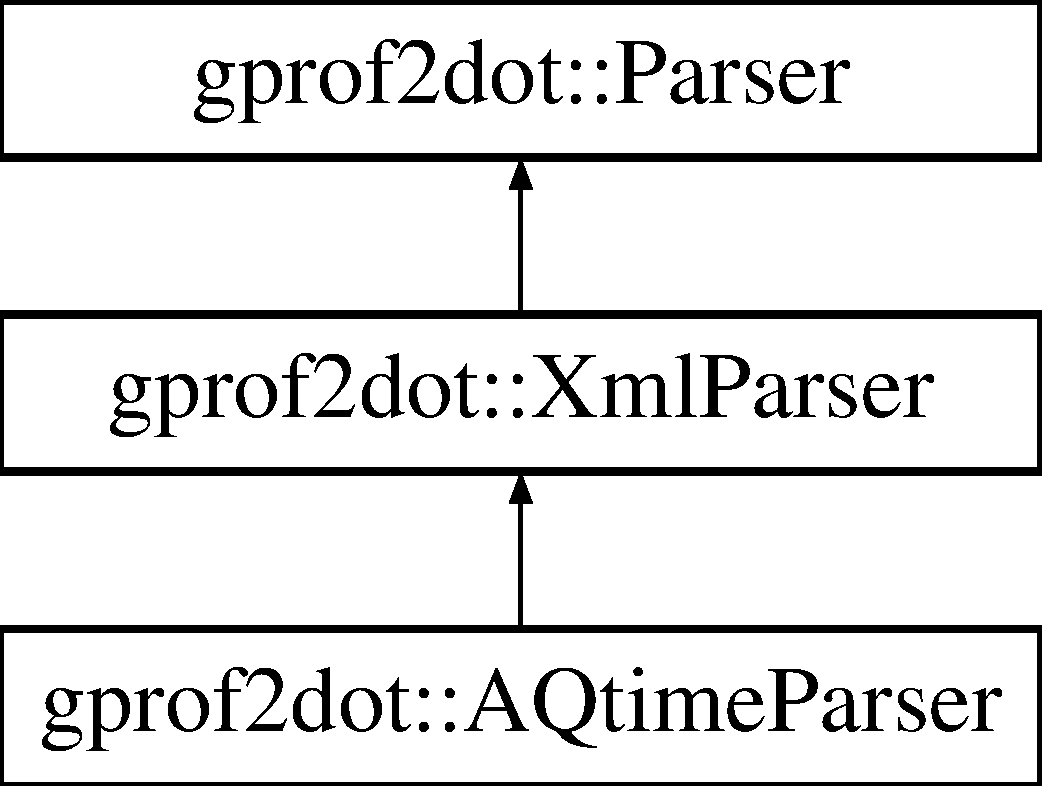
\includegraphics[height=3.000000cm]{classgprof2dot_1_1AQtimeParser}
\end{center}
\end{figure}
\subsection*{Public Member Functions}
\begin{DoxyCompactItemize}
\item 
def \hyperlink{classgprof2dot_1_1AQtimeParser_aa59b49fada6b1c6fe520c4a54bca5e77}{\_\-\_\-init\_\-\_\-}
\item 
def \hyperlink{classgprof2dot_1_1AQtimeParser_ab1e9b6f7ddff3943366aba840235aa87}{parse}
\item 
def \hyperlink{classgprof2dot_1_1AQtimeParser_a0dee761c0b4c61e560bb1c3f072b741c}{parse\_\-headers}
\item 
def \hyperlink{classgprof2dot_1_1AQtimeParser_a04bf6c338f7dc92014aee30551531084}{parse\_\-table\_\-header}
\item 
def \hyperlink{classgprof2dot_1_1AQtimeParser_a48f22b51e594042737d0981c176ab6b8}{parse\_\-table\_\-field}
\item 
def \hyperlink{classgprof2dot_1_1AQtimeParser_a32b9f835b37afe23ec4625056d362aa3}{parse\_\-results}
\item 
def \hyperlink{classgprof2dot_1_1AQtimeParser_a8be190969437a5e4bb7fb9e23de6f65a}{parse\_\-data}
\item 
def \hyperlink{classgprof2dot_1_1AQtimeParser_ac0a6dae6925c42090428a57e4a12f58a}{parse\_\-row}
\item 
def \hyperlink{classgprof2dot_1_1AQtimeParser_a41f9d9db95c1bef28c89d9f4751b78ce}{parse\_\-field}
\item 
def \hyperlink{classgprof2dot_1_1AQtimeParser_a13b6a9afdad05501c9d8ca29d1b12181}{parse\_\-children}
\item 
def \hyperlink{classgprof2dot_1_1AQtimeParser_a73e031867ccede4d5134a237a0557d7b}{build\_\-profile}
\item 
def \hyperlink{classgprof2dot_1_1AQtimeParser_adb9096422670b456f863289f353a1442}{build\_\-function}
\item 
def \hyperlink{classgprof2dot_1_1AQtimeParser_a46b68311d7b2c1a49c920df87a43b15c}{build\_\-call}
\item 
def \hyperlink{classgprof2dot_1_1AQtimeParser_a0523f5cca159ef16101c9db5a05dcc7e}{build\_\-id}
\item 
def \hyperlink{classgprof2dot_1_1AQtimeParser_ad6570e9c5dbbd6902762c915058eb086}{build\_\-name}
\end{DoxyCompactItemize}
\subsection*{Public Attributes}
\begin{DoxyCompactItemize}
\item 
\hyperlink{classgprof2dot_1_1AQtimeParser_a9710b990cfcffca84b59c036e713868e}{tables}
\end{DoxyCompactItemize}


\subsection{Constructor \& Destructor Documentation}
\hypertarget{classgprof2dot_1_1AQtimeParser_aa59b49fada6b1c6fe520c4a54bca5e77}{
\index{gprof2dot::AQtimeParser@{gprof2dot::AQtimeParser}!\_\-\_\-init\_\-\_\-@{\_\-\_\-init\_\-\_\-}}
\index{\_\-\_\-init\_\-\_\-@{\_\-\_\-init\_\-\_\-}!gprof2dot::AQtimeParser@{gprof2dot::AQtimeParser}}
\subsubsection[{\_\-\_\-init\_\-\_\-}]{\setlength{\rightskip}{0pt plus 5cm}def gprof2dot::AQtimeParser::\_\-\_\-init\_\-\_\- (
\begin{DoxyParamCaption}
\item[{}]{self, }
\item[{}]{stream}
\end{DoxyParamCaption}
)}}
\label{classgprof2dot_1_1AQtimeParser_aa59b49fada6b1c6fe520c4a54bca5e77}


Reimplemented from \hyperlink{classgprof2dot_1_1XmlParser_ac3307ca05e7e17b5b6a2b96e9782107e}{gprof2dot::XmlParser}.



\subsection{Member Function Documentation}
\hypertarget{classgprof2dot_1_1AQtimeParser_a46b68311d7b2c1a49c920df87a43b15c}{
\index{gprof2dot::AQtimeParser@{gprof2dot::AQtimeParser}!build\_\-call@{build\_\-call}}
\index{build\_\-call@{build\_\-call}!gprof2dot::AQtimeParser@{gprof2dot::AQtimeParser}}
\subsubsection[{build\_\-call}]{\setlength{\rightskip}{0pt plus 5cm}def gprof2dot::AQtimeParser::build\_\-call (
\begin{DoxyParamCaption}
\item[{}]{self, }
\item[{}]{fields}
\end{DoxyParamCaption}
)}}
\label{classgprof2dot_1_1AQtimeParser_a46b68311d7b2c1a49c920df87a43b15c}
\hypertarget{classgprof2dot_1_1AQtimeParser_adb9096422670b456f863289f353a1442}{
\index{gprof2dot::AQtimeParser@{gprof2dot::AQtimeParser}!build\_\-function@{build\_\-function}}
\index{build\_\-function@{build\_\-function}!gprof2dot::AQtimeParser@{gprof2dot::AQtimeParser}}
\subsubsection[{build\_\-function}]{\setlength{\rightskip}{0pt plus 5cm}def gprof2dot::AQtimeParser::build\_\-function (
\begin{DoxyParamCaption}
\item[{}]{self, }
\item[{}]{fields}
\end{DoxyParamCaption}
)}}
\label{classgprof2dot_1_1AQtimeParser_adb9096422670b456f863289f353a1442}
\hypertarget{classgprof2dot_1_1AQtimeParser_a0523f5cca159ef16101c9db5a05dcc7e}{
\index{gprof2dot::AQtimeParser@{gprof2dot::AQtimeParser}!build\_\-id@{build\_\-id}}
\index{build\_\-id@{build\_\-id}!gprof2dot::AQtimeParser@{gprof2dot::AQtimeParser}}
\subsubsection[{build\_\-id}]{\setlength{\rightskip}{0pt plus 5cm}def gprof2dot::AQtimeParser::build\_\-id (
\begin{DoxyParamCaption}
\item[{}]{self, }
\item[{}]{fields}
\end{DoxyParamCaption}
)}}
\label{classgprof2dot_1_1AQtimeParser_a0523f5cca159ef16101c9db5a05dcc7e}
\hypertarget{classgprof2dot_1_1AQtimeParser_ad6570e9c5dbbd6902762c915058eb086}{
\index{gprof2dot::AQtimeParser@{gprof2dot::AQtimeParser}!build\_\-name@{build\_\-name}}
\index{build\_\-name@{build\_\-name}!gprof2dot::AQtimeParser@{gprof2dot::AQtimeParser}}
\subsubsection[{build\_\-name}]{\setlength{\rightskip}{0pt plus 5cm}def gprof2dot::AQtimeParser::build\_\-name (
\begin{DoxyParamCaption}
\item[{}]{self, }
\item[{}]{fields}
\end{DoxyParamCaption}
)}}
\label{classgprof2dot_1_1AQtimeParser_ad6570e9c5dbbd6902762c915058eb086}
\hypertarget{classgprof2dot_1_1AQtimeParser_a73e031867ccede4d5134a237a0557d7b}{
\index{gprof2dot::AQtimeParser@{gprof2dot::AQtimeParser}!build\_\-profile@{build\_\-profile}}
\index{build\_\-profile@{build\_\-profile}!gprof2dot::AQtimeParser@{gprof2dot::AQtimeParser}}
\subsubsection[{build\_\-profile}]{\setlength{\rightskip}{0pt plus 5cm}def gprof2dot::AQtimeParser::build\_\-profile (
\begin{DoxyParamCaption}
\item[{}]{self, }
\item[{}]{results}
\end{DoxyParamCaption}
)}}
\label{classgprof2dot_1_1AQtimeParser_a73e031867ccede4d5134a237a0557d7b}
\hypertarget{classgprof2dot_1_1AQtimeParser_ab1e9b6f7ddff3943366aba840235aa87}{
\index{gprof2dot::AQtimeParser@{gprof2dot::AQtimeParser}!parse@{parse}}
\index{parse@{parse}!gprof2dot::AQtimeParser@{gprof2dot::AQtimeParser}}
\subsubsection[{parse}]{\setlength{\rightskip}{0pt plus 5cm}def gprof2dot::AQtimeParser::parse (
\begin{DoxyParamCaption}
\item[{}]{self}
\end{DoxyParamCaption}
)}}
\label{classgprof2dot_1_1AQtimeParser_ab1e9b6f7ddff3943366aba840235aa87}


Reimplemented from \hyperlink{classgprof2dot_1_1Parser_a681a0bc74e640c9c8e3d629dd03049fc}{gprof2dot::Parser}.

\hypertarget{classgprof2dot_1_1AQtimeParser_a13b6a9afdad05501c9d8ca29d1b12181}{
\index{gprof2dot::AQtimeParser@{gprof2dot::AQtimeParser}!parse\_\-children@{parse\_\-children}}
\index{parse\_\-children@{parse\_\-children}!gprof2dot::AQtimeParser@{gprof2dot::AQtimeParser}}
\subsubsection[{parse\_\-children}]{\setlength{\rightskip}{0pt plus 5cm}def gprof2dot::AQtimeParser::parse\_\-children (
\begin{DoxyParamCaption}
\item[{}]{self}
\end{DoxyParamCaption}
)}}
\label{classgprof2dot_1_1AQtimeParser_a13b6a9afdad05501c9d8ca29d1b12181}
\hypertarget{classgprof2dot_1_1AQtimeParser_a8be190969437a5e4bb7fb9e23de6f65a}{
\index{gprof2dot::AQtimeParser@{gprof2dot::AQtimeParser}!parse\_\-data@{parse\_\-data}}
\index{parse\_\-data@{parse\_\-data}!gprof2dot::AQtimeParser@{gprof2dot::AQtimeParser}}
\subsubsection[{parse\_\-data}]{\setlength{\rightskip}{0pt plus 5cm}def gprof2dot::AQtimeParser::parse\_\-data (
\begin{DoxyParamCaption}
\item[{}]{self}
\end{DoxyParamCaption}
)}}
\label{classgprof2dot_1_1AQtimeParser_a8be190969437a5e4bb7fb9e23de6f65a}
\hypertarget{classgprof2dot_1_1AQtimeParser_a41f9d9db95c1bef28c89d9f4751b78ce}{
\index{gprof2dot::AQtimeParser@{gprof2dot::AQtimeParser}!parse\_\-field@{parse\_\-field}}
\index{parse\_\-field@{parse\_\-field}!gprof2dot::AQtimeParser@{gprof2dot::AQtimeParser}}
\subsubsection[{parse\_\-field}]{\setlength{\rightskip}{0pt plus 5cm}def gprof2dot::AQtimeParser::parse\_\-field (
\begin{DoxyParamCaption}
\item[{}]{self, }
\item[{}]{field\_\-types}
\end{DoxyParamCaption}
)}}
\label{classgprof2dot_1_1AQtimeParser_a41f9d9db95c1bef28c89d9f4751b78ce}
\hypertarget{classgprof2dot_1_1AQtimeParser_a0dee761c0b4c61e560bb1c3f072b741c}{
\index{gprof2dot::AQtimeParser@{gprof2dot::AQtimeParser}!parse\_\-headers@{parse\_\-headers}}
\index{parse\_\-headers@{parse\_\-headers}!gprof2dot::AQtimeParser@{gprof2dot::AQtimeParser}}
\subsubsection[{parse\_\-headers}]{\setlength{\rightskip}{0pt plus 5cm}def gprof2dot::AQtimeParser::parse\_\-headers (
\begin{DoxyParamCaption}
\item[{}]{self}
\end{DoxyParamCaption}
)}}
\label{classgprof2dot_1_1AQtimeParser_a0dee761c0b4c61e560bb1c3f072b741c}
\hypertarget{classgprof2dot_1_1AQtimeParser_a32b9f835b37afe23ec4625056d362aa3}{
\index{gprof2dot::AQtimeParser@{gprof2dot::AQtimeParser}!parse\_\-results@{parse\_\-results}}
\index{parse\_\-results@{parse\_\-results}!gprof2dot::AQtimeParser@{gprof2dot::AQtimeParser}}
\subsubsection[{parse\_\-results}]{\setlength{\rightskip}{0pt plus 5cm}def gprof2dot::AQtimeParser::parse\_\-results (
\begin{DoxyParamCaption}
\item[{}]{self}
\end{DoxyParamCaption}
)}}
\label{classgprof2dot_1_1AQtimeParser_a32b9f835b37afe23ec4625056d362aa3}
\hypertarget{classgprof2dot_1_1AQtimeParser_ac0a6dae6925c42090428a57e4a12f58a}{
\index{gprof2dot::AQtimeParser@{gprof2dot::AQtimeParser}!parse\_\-row@{parse\_\-row}}
\index{parse\_\-row@{parse\_\-row}!gprof2dot::AQtimeParser@{gprof2dot::AQtimeParser}}
\subsubsection[{parse\_\-row}]{\setlength{\rightskip}{0pt plus 5cm}def gprof2dot::AQtimeParser::parse\_\-row (
\begin{DoxyParamCaption}
\item[{}]{self, }
\item[{}]{field\_\-types}
\end{DoxyParamCaption}
)}}
\label{classgprof2dot_1_1AQtimeParser_ac0a6dae6925c42090428a57e4a12f58a}
\hypertarget{classgprof2dot_1_1AQtimeParser_a48f22b51e594042737d0981c176ab6b8}{
\index{gprof2dot::AQtimeParser@{gprof2dot::AQtimeParser}!parse\_\-table\_\-field@{parse\_\-table\_\-field}}
\index{parse\_\-table\_\-field@{parse\_\-table\_\-field}!gprof2dot::AQtimeParser@{gprof2dot::AQtimeParser}}
\subsubsection[{parse\_\-table\_\-field}]{\setlength{\rightskip}{0pt plus 5cm}def gprof2dot::AQtimeParser::parse\_\-table\_\-field (
\begin{DoxyParamCaption}
\item[{}]{self}
\end{DoxyParamCaption}
)}}
\label{classgprof2dot_1_1AQtimeParser_a48f22b51e594042737d0981c176ab6b8}
\hypertarget{classgprof2dot_1_1AQtimeParser_a04bf6c338f7dc92014aee30551531084}{
\index{gprof2dot::AQtimeParser@{gprof2dot::AQtimeParser}!parse\_\-table\_\-header@{parse\_\-table\_\-header}}
\index{parse\_\-table\_\-header@{parse\_\-table\_\-header}!gprof2dot::AQtimeParser@{gprof2dot::AQtimeParser}}
\subsubsection[{parse\_\-table\_\-header}]{\setlength{\rightskip}{0pt plus 5cm}def gprof2dot::AQtimeParser::parse\_\-table\_\-header (
\begin{DoxyParamCaption}
\item[{}]{self}
\end{DoxyParamCaption}
)}}
\label{classgprof2dot_1_1AQtimeParser_a04bf6c338f7dc92014aee30551531084}


\subsection{Member Data Documentation}
\hypertarget{classgprof2dot_1_1AQtimeParser_a9710b990cfcffca84b59c036e713868e}{
\index{gprof2dot::AQtimeParser@{gprof2dot::AQtimeParser}!tables@{tables}}
\index{tables@{tables}!gprof2dot::AQtimeParser@{gprof2dot::AQtimeParser}}
\subsubsection[{tables}]{\setlength{\rightskip}{0pt plus 5cm}{\bf gprof2dot::AQtimeParser::tables}}}
\label{classgprof2dot_1_1AQtimeParser_a9710b990cfcffca84b59c036e713868e}


The documentation for this class was generated from the following file:\begin{DoxyCompactItemize}
\item 
\hyperlink{gprof2dot_8py}{gprof2dot.py}\end{DoxyCompactItemize}

\hypertarget{classgprof2dot_1_1AQtimeTable}{
\section{gprof2dot::AQtimeTable Class Reference}
\label{classgprof2dot_1_1AQtimeTable}\index{gprof2dot::AQtimeTable@{gprof2dot::AQtimeTable}}
}
\subsection*{Public Member Functions}
\begin{DoxyCompactItemize}
\item 
def \hyperlink{classgprof2dot_1_1AQtimeTable_aa4471b964aee946156802814b0b05a72}{\_\-\_\-init\_\-\_\-}
\item 
def \hyperlink{classgprof2dot_1_1AQtimeTable_a8d883b1c9051dd3fd069e504447d5819}{\_\-\_\-len\_\-\_\-}
\item 
def \hyperlink{classgprof2dot_1_1AQtimeTable_a02a9525c798326375b27d8a92ebf7a3c}{\_\-\_\-iter\_\-\_\-}
\item 
def \hyperlink{classgprof2dot_1_1AQtimeTable_aa94f5f1f213161bca97429c6c7290079}{add\_\-row}
\end{DoxyCompactItemize}
\subsection*{Public Attributes}
\begin{DoxyCompactItemize}
\item 
\hyperlink{classgprof2dot_1_1AQtimeTable_a36f271c4d80be0942ce35174f970595c}{name}
\item 
\hyperlink{classgprof2dot_1_1AQtimeTable_a3351d141678983f6f15f2f046b695d2e}{fields}
\item 
\hyperlink{classgprof2dot_1_1AQtimeTable_adc0ff5163091ffbe7552b25ff26acd59}{field\_\-column}
\item 
\hyperlink{classgprof2dot_1_1AQtimeTable_af63945349bbb65571ac283eb68ea50dc}{rows}
\end{DoxyCompactItemize}


\subsection{Constructor \& Destructor Documentation}
\hypertarget{classgprof2dot_1_1AQtimeTable_aa4471b964aee946156802814b0b05a72}{
\index{gprof2dot::AQtimeTable@{gprof2dot::AQtimeTable}!\_\-\_\-init\_\-\_\-@{\_\-\_\-init\_\-\_\-}}
\index{\_\-\_\-init\_\-\_\-@{\_\-\_\-init\_\-\_\-}!gprof2dot::AQtimeTable@{gprof2dot::AQtimeTable}}
\subsubsection[{\_\-\_\-init\_\-\_\-}]{\setlength{\rightskip}{0pt plus 5cm}def gprof2dot::AQtimeTable::\_\-\_\-init\_\-\_\- (
\begin{DoxyParamCaption}
\item[{}]{self, }
\item[{}]{name, }
\item[{}]{fields}
\end{DoxyParamCaption}
)}}
\label{classgprof2dot_1_1AQtimeTable_aa4471b964aee946156802814b0b05a72}


\subsection{Member Function Documentation}
\hypertarget{classgprof2dot_1_1AQtimeTable_a02a9525c798326375b27d8a92ebf7a3c}{
\index{gprof2dot::AQtimeTable@{gprof2dot::AQtimeTable}!\_\-\_\-iter\_\-\_\-@{\_\-\_\-iter\_\-\_\-}}
\index{\_\-\_\-iter\_\-\_\-@{\_\-\_\-iter\_\-\_\-}!gprof2dot::AQtimeTable@{gprof2dot::AQtimeTable}}
\subsubsection[{\_\-\_\-iter\_\-\_\-}]{\setlength{\rightskip}{0pt plus 5cm}def gprof2dot::AQtimeTable::\_\-\_\-iter\_\-\_\- (
\begin{DoxyParamCaption}
\item[{}]{self}
\end{DoxyParamCaption}
)}}
\label{classgprof2dot_1_1AQtimeTable_a02a9525c798326375b27d8a92ebf7a3c}
\hypertarget{classgprof2dot_1_1AQtimeTable_a8d883b1c9051dd3fd069e504447d5819}{
\index{gprof2dot::AQtimeTable@{gprof2dot::AQtimeTable}!\_\-\_\-len\_\-\_\-@{\_\-\_\-len\_\-\_\-}}
\index{\_\-\_\-len\_\-\_\-@{\_\-\_\-len\_\-\_\-}!gprof2dot::AQtimeTable@{gprof2dot::AQtimeTable}}
\subsubsection[{\_\-\_\-len\_\-\_\-}]{\setlength{\rightskip}{0pt plus 5cm}def gprof2dot::AQtimeTable::\_\-\_\-len\_\-\_\- (
\begin{DoxyParamCaption}
\item[{}]{self}
\end{DoxyParamCaption}
)}}
\label{classgprof2dot_1_1AQtimeTable_a8d883b1c9051dd3fd069e504447d5819}
\hypertarget{classgprof2dot_1_1AQtimeTable_aa94f5f1f213161bca97429c6c7290079}{
\index{gprof2dot::AQtimeTable@{gprof2dot::AQtimeTable}!add\_\-row@{add\_\-row}}
\index{add\_\-row@{add\_\-row}!gprof2dot::AQtimeTable@{gprof2dot::AQtimeTable}}
\subsubsection[{add\_\-row}]{\setlength{\rightskip}{0pt plus 5cm}def gprof2dot::AQtimeTable::add\_\-row (
\begin{DoxyParamCaption}
\item[{}]{self, }
\item[{}]{values, }
\item[{}]{children = {\ttfamily ()}}
\end{DoxyParamCaption}
)}}
\label{classgprof2dot_1_1AQtimeTable_aa94f5f1f213161bca97429c6c7290079}


\subsection{Member Data Documentation}
\hypertarget{classgprof2dot_1_1AQtimeTable_adc0ff5163091ffbe7552b25ff26acd59}{
\index{gprof2dot::AQtimeTable@{gprof2dot::AQtimeTable}!field\_\-column@{field\_\-column}}
\index{field\_\-column@{field\_\-column}!gprof2dot::AQtimeTable@{gprof2dot::AQtimeTable}}
\subsubsection[{field\_\-column}]{\setlength{\rightskip}{0pt plus 5cm}{\bf gprof2dot::AQtimeTable::field\_\-column}}}
\label{classgprof2dot_1_1AQtimeTable_adc0ff5163091ffbe7552b25ff26acd59}
\hypertarget{classgprof2dot_1_1AQtimeTable_a3351d141678983f6f15f2f046b695d2e}{
\index{gprof2dot::AQtimeTable@{gprof2dot::AQtimeTable}!fields@{fields}}
\index{fields@{fields}!gprof2dot::AQtimeTable@{gprof2dot::AQtimeTable}}
\subsubsection[{fields}]{\setlength{\rightskip}{0pt plus 5cm}{\bf gprof2dot::AQtimeTable::fields}}}
\label{classgprof2dot_1_1AQtimeTable_a3351d141678983f6f15f2f046b695d2e}
\hypertarget{classgprof2dot_1_1AQtimeTable_a36f271c4d80be0942ce35174f970595c}{
\index{gprof2dot::AQtimeTable@{gprof2dot::AQtimeTable}!name@{name}}
\index{name@{name}!gprof2dot::AQtimeTable@{gprof2dot::AQtimeTable}}
\subsubsection[{name}]{\setlength{\rightskip}{0pt plus 5cm}{\bf gprof2dot::AQtimeTable::name}}}
\label{classgprof2dot_1_1AQtimeTable_a36f271c4d80be0942ce35174f970595c}
\hypertarget{classgprof2dot_1_1AQtimeTable_af63945349bbb65571ac283eb68ea50dc}{
\index{gprof2dot::AQtimeTable@{gprof2dot::AQtimeTable}!rows@{rows}}
\index{rows@{rows}!gprof2dot::AQtimeTable@{gprof2dot::AQtimeTable}}
\subsubsection[{rows}]{\setlength{\rightskip}{0pt plus 5cm}{\bf gprof2dot::AQtimeTable::rows}}}
\label{classgprof2dot_1_1AQtimeTable_af63945349bbb65571ac283eb68ea50dc}


The documentation for this class was generated from the following file:\begin{DoxyCompactItemize}
\item 
\hyperlink{gprof2dot_8py}{gprof2dot.py}\end{DoxyCompactItemize}

\hypertarget{classBgCommand}{
\section{BgCommand Class Reference}
\label{classBgCommand}\index{BgCommand@{BgCommand}}
}


Classe que implementa o comando bg.  




{\ttfamily \#include $<$Builtin.hpp$>$}

Inheritance diagram for BgCommand:\begin{figure}[H]
\begin{center}
\leavevmode
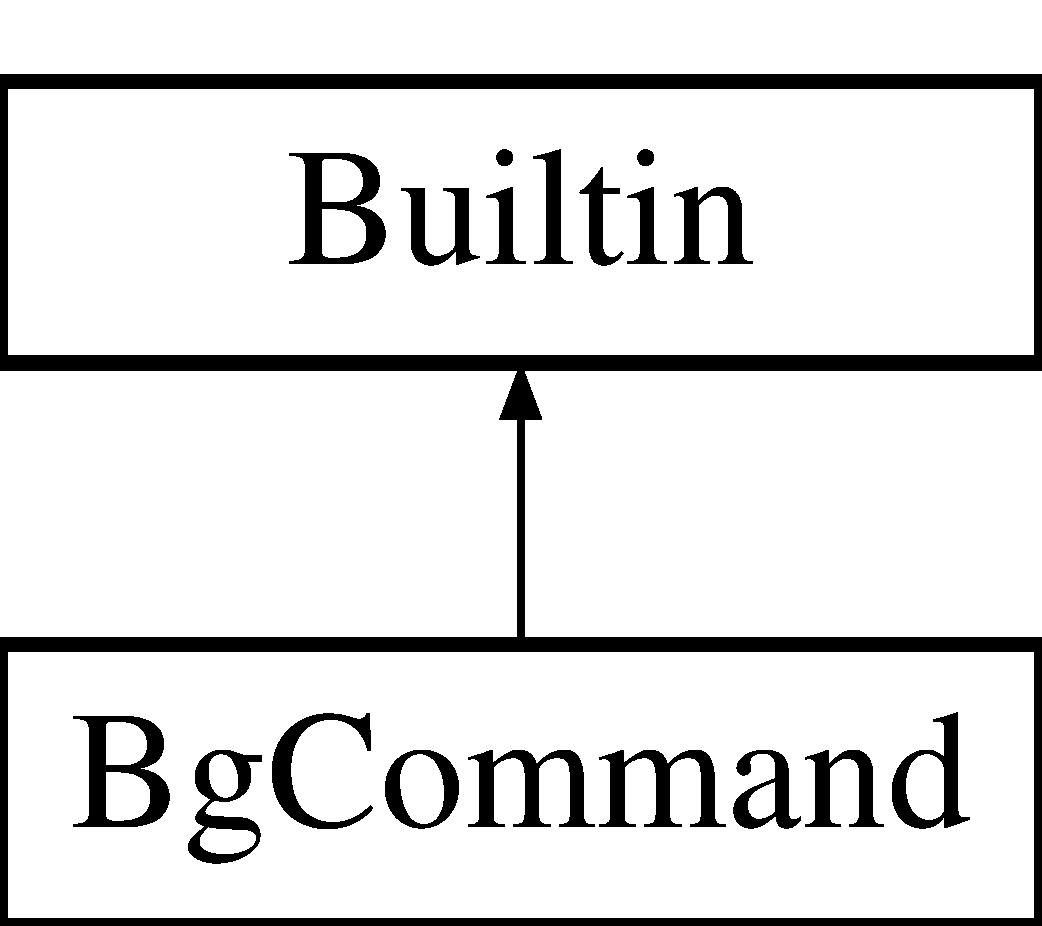
\includegraphics[height=2.000000cm]{classBgCommand}
\end{center}
\end{figure}


\subsection{Detailed Description}
Classe que implementa o comando bg. Sintaxe: bg \%$<$JOBID$>$ $|$ bg\par
 Se o comando for chamado sem o JOBID, sera utilizado o job mais recentemente aberto, colocado em foreground ou background ou, caso ja tenha sido fechado, o mais antigo aberto. 

The documentation for this class was generated from the following files:\begin{DoxyCompactItemize}
\item 
\hyperlink{Builtin_8hpp}{Builtin.hpp}\item 
\hyperlink{Builtin_8cpp}{Builtin.cpp}\end{DoxyCompactItemize}

\hypertarget{classBuiltin}{
\section{Builtin Class Reference}
\label{classBuiltin}\index{Builtin@{Builtin}}
}


{\ttfamily \#include $<$Builtin.hpp$>$}

Inheritance diagram for Builtin:\begin{figure}[H]
\begin{center}
\leavevmode
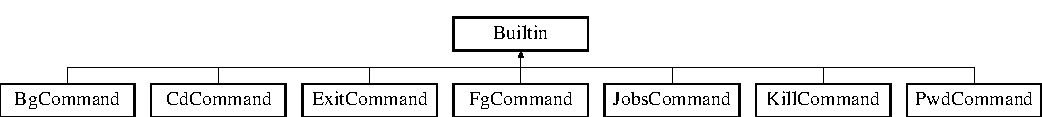
\includegraphics[height=1.568627cm]{classBuiltin}
\end{center}
\end{figure}
\subsection*{Public Member Functions}
\begin{DoxyCompactItemize}
\item 
void \hyperlink{classBuiltin_aeb4e6144d47e07c4afedb20ee66671be}{run} (const char $\ast$\mbox{[}$\,$\mbox{]}, \hyperlink{classExecutor}{Executor} $\ast$)
\item 
virtual bool \hyperlink{classBuiltin_a91ec773bbed5e1a8808955d9b48e664b}{forkable} ()
\end{DoxyCompactItemize}


\subsection{Member Function Documentation}
\hypertarget{classBuiltin_a91ec773bbed5e1a8808955d9b48e664b}{
\index{Builtin@{Builtin}!forkable@{forkable}}
\index{forkable@{forkable}!Builtin@{Builtin}}
\subsubsection[{forkable}]{\setlength{\rightskip}{0pt plus 5cm}bool Builtin::forkable (
\begin{DoxyParamCaption}
{}
\end{DoxyParamCaption}
)\hspace{0.3cm}{\ttfamily  \mbox{[}virtual\mbox{]}}}}
\label{classBuiltin_a91ec773bbed5e1a8808955d9b48e664b}
\hypertarget{classBuiltin_aeb4e6144d47e07c4afedb20ee66671be}{
\index{Builtin@{Builtin}!run@{run}}
\index{run@{run}!Builtin@{Builtin}}
\subsubsection[{run}]{\setlength{\rightskip}{0pt plus 5cm}void Builtin::run (
\begin{DoxyParamCaption}
\item[{const char $\ast$}]{args\mbox{[}$\,$\mbox{]}, }
\item[{{\bf Executor} $\ast$}]{executor}
\end{DoxyParamCaption}
)}}
\label{classBuiltin_aeb4e6144d47e07c4afedb20ee66671be}


The documentation for this class was generated from the following files:\begin{DoxyCompactItemize}
\item 
\hyperlink{Builtin_8hpp}{Builtin.hpp}\item 
\hyperlink{Builtin_8cpp}{Builtin.cpp}\end{DoxyCompactItemize}

\hypertarget{classgprof2dot_1_1Call}{
\section{gprof2dot::Call Class Reference}
\label{classgprof2dot_1_1Call}\index{gprof2dot::Call@{gprof2dot::Call}}
}
Inheritance diagram for gprof2dot::Call:\begin{figure}[H]
\begin{center}
\leavevmode
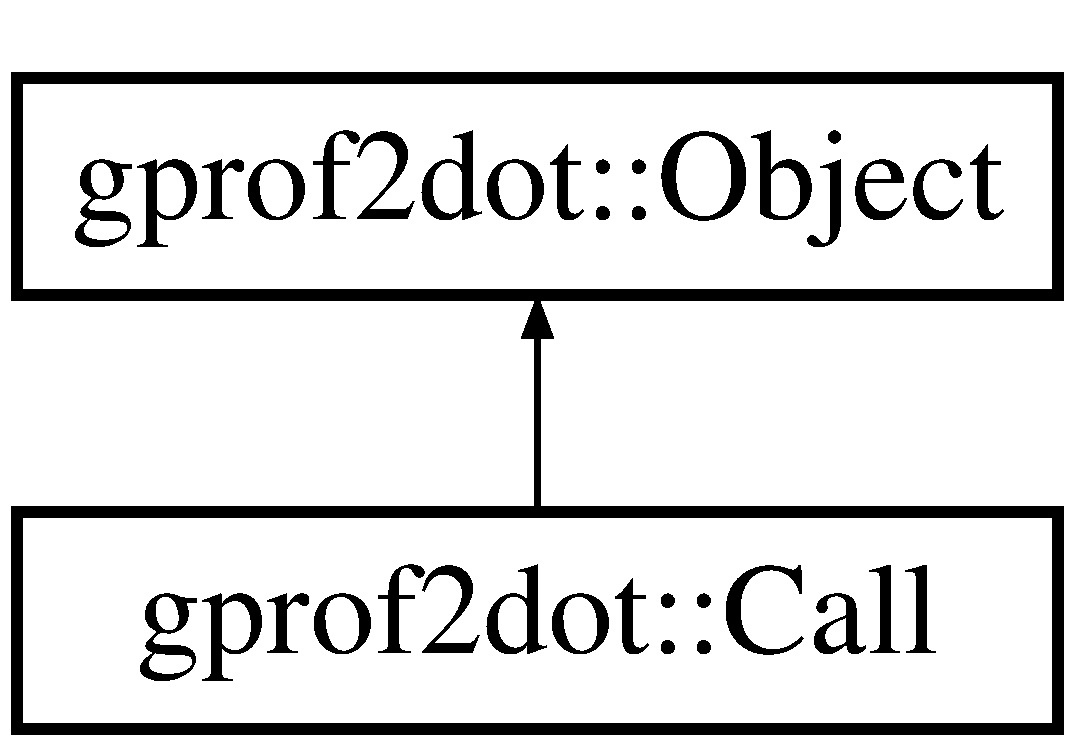
\includegraphics[height=2.000000cm]{classgprof2dot_1_1Call}
\end{center}
\end{figure}
\subsection*{Public Member Functions}
\begin{DoxyCompactItemize}
\item 
def \hyperlink{classgprof2dot_1_1Call_a2e6af456964a01d7fa4768224fbf729c}{\_\-\_\-init\_\-\_\-}
\end{DoxyCompactItemize}
\subsection*{Public Attributes}
\begin{DoxyCompactItemize}
\item 
\hyperlink{classgprof2dot_1_1Call_ac28cb11c1eb7879b1d4d1c7d565b4f4e}{callee\_\-id}
\item 
\hyperlink{classgprof2dot_1_1Call_ad8b10e2156b9956184d55d4848721c93}{ratio}
\item 
\hyperlink{classgprof2dot_1_1Call_ab112a157165a7e938383281eb8754830}{weight}
\end{DoxyCompactItemize}


\subsection{Detailed Description}
\begin{DoxyVerb}A call between functions.

There should be at most one call object for every pair of functions.
\end{DoxyVerb}
 

\subsection{Constructor \& Destructor Documentation}
\hypertarget{classgprof2dot_1_1Call_a2e6af456964a01d7fa4768224fbf729c}{
\index{gprof2dot::Call@{gprof2dot::Call}!\_\-\_\-init\_\-\_\-@{\_\-\_\-init\_\-\_\-}}
\index{\_\-\_\-init\_\-\_\-@{\_\-\_\-init\_\-\_\-}!gprof2dot::Call@{gprof2dot::Call}}
\subsubsection[{\_\-\_\-init\_\-\_\-}]{\setlength{\rightskip}{0pt plus 5cm}def gprof2dot::Call::\_\-\_\-init\_\-\_\- (
\begin{DoxyParamCaption}
\item[{}]{self, }
\item[{}]{callee\_\-id}
\end{DoxyParamCaption}
)}}
\label{classgprof2dot_1_1Call_a2e6af456964a01d7fa4768224fbf729c}


Reimplemented from \hyperlink{classgprof2dot_1_1Object_ae98eed8f428fdb899a83c5a659346c33}{gprof2dot::Object}.



\subsection{Member Data Documentation}
\hypertarget{classgprof2dot_1_1Call_ac28cb11c1eb7879b1d4d1c7d565b4f4e}{
\index{gprof2dot::Call@{gprof2dot::Call}!callee\_\-id@{callee\_\-id}}
\index{callee\_\-id@{callee\_\-id}!gprof2dot::Call@{gprof2dot::Call}}
\subsubsection[{callee\_\-id}]{\setlength{\rightskip}{0pt plus 5cm}{\bf gprof2dot::Call::callee\_\-id}}}
\label{classgprof2dot_1_1Call_ac28cb11c1eb7879b1d4d1c7d565b4f4e}
\hypertarget{classgprof2dot_1_1Call_ad8b10e2156b9956184d55d4848721c93}{
\index{gprof2dot::Call@{gprof2dot::Call}!ratio@{ratio}}
\index{ratio@{ratio}!gprof2dot::Call@{gprof2dot::Call}}
\subsubsection[{ratio}]{\setlength{\rightskip}{0pt plus 5cm}{\bf gprof2dot::Call::ratio}}}
\label{classgprof2dot_1_1Call_ad8b10e2156b9956184d55d4848721c93}
\hypertarget{classgprof2dot_1_1Call_ab112a157165a7e938383281eb8754830}{
\index{gprof2dot::Call@{gprof2dot::Call}!weight@{weight}}
\index{weight@{weight}!gprof2dot::Call@{gprof2dot::Call}}
\subsubsection[{weight}]{\setlength{\rightskip}{0pt plus 5cm}{\bf gprof2dot::Call::weight}}}
\label{classgprof2dot_1_1Call_ab112a157165a7e938383281eb8754830}


The documentation for this class was generated from the following file:\begin{DoxyCompactItemize}
\item 
\hyperlink{gprof2dot_8py}{gprof2dot.py}\end{DoxyCompactItemize}

\hypertarget{classgprof2dot_1_1CallgrindParser}{
\section{gprof2dot::CallgrindParser Class Reference}
\label{classgprof2dot_1_1CallgrindParser}\index{gprof2dot::CallgrindParser@{gprof2dot::CallgrindParser}}
}
Inheritance diagram for gprof2dot::CallgrindParser:\begin{figure}[H]
\begin{center}
\leavevmode
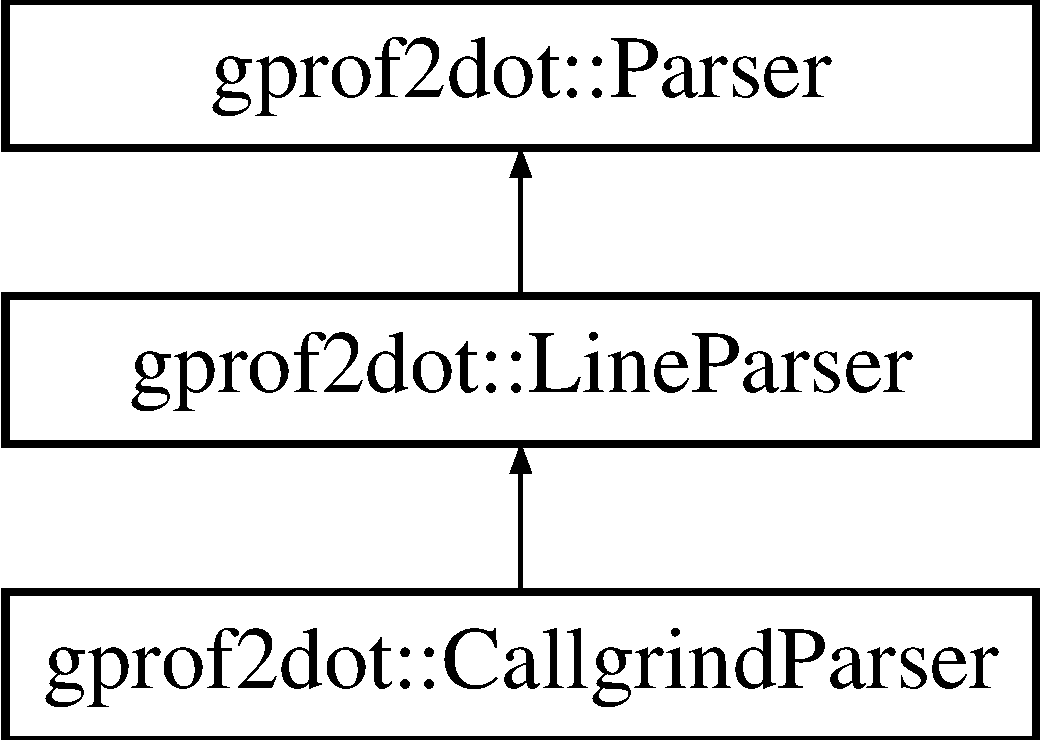
\includegraphics[height=3.000000cm]{classgprof2dot_1_1CallgrindParser}
\end{center}
\end{figure}
\subsection*{Public Member Functions}
\begin{DoxyCompactItemize}
\item 
def \hyperlink{classgprof2dot_1_1CallgrindParser_a05844f0101a68e1f532064b78f5e2dfa}{\_\-\_\-init\_\-\_\-}
\item 
def \hyperlink{classgprof2dot_1_1CallgrindParser_ad5ef0ee6f7e2c0987f49452ef1488ea0}{parse}
\item 
def \hyperlink{classgprof2dot_1_1CallgrindParser_a166c364691bdfc631658e2d8d44207ae}{parse\_\-part}
\item 
def \hyperlink{classgprof2dot_1_1CallgrindParser_af374e0f657409ad7cd105f7aae5fcf22}{parse\_\-header\_\-line}
\item 
def \hyperlink{classgprof2dot_1_1CallgrindParser_a8cfe8d654d63be805492d5fcfcc981c9}{parse\_\-part\_\-detail}
\item 
def \hyperlink{classgprof2dot_1_1CallgrindParser_ae6400928371af8dde77bf0781c7a0e64}{parse\_\-description}
\item 
def \hyperlink{classgprof2dot_1_1CallgrindParser_ae3af3ac1f897f439ec133b283a9471af}{parse\_\-event\_\-specification}
\item 
def \hyperlink{classgprof2dot_1_1CallgrindParser_a5ed9361ca6523750266321cfd9cb6cb8}{parse\_\-cost\_\-line\_\-def}
\item 
def \hyperlink{classgprof2dot_1_1CallgrindParser_a2fdb90e13dc60949beecdc3e24f08614}{parse\_\-cost\_\-summary}
\item 
def \hyperlink{classgprof2dot_1_1CallgrindParser_a74fe82afe9a469adea0dd5c8847370b7}{parse\_\-body\_\-line}
\item 
def \hyperlink{classgprof2dot_1_1CallgrindParser_a206aecc896d7c1f80fe5726d32eff675}{parse\_\-cost\_\-line}
\item 
def \hyperlink{classgprof2dot_1_1CallgrindParser_a5798c71d43205ef6221ccd1b68482208}{parse\_\-association\_\-spec}
\item 
def \hyperlink{classgprof2dot_1_1CallgrindParser_a43de4d71d555469b7b50ee32d863dba6}{parse\_\-position\_\-spec}
\item 
def \hyperlink{classgprof2dot_1_1CallgrindParser_a81563826fed7fcd84d84f8cbf1e160a3}{parse\_\-empty}
\item 
def \hyperlink{classgprof2dot_1_1CallgrindParser_aa5e679c2a5cf0a55f7aec259b99382fe}{parse\_\-comment}
\item 
def \hyperlink{classgprof2dot_1_1CallgrindParser_a2a304d826b3709be02c59a516394ea59}{parse\_\-key}
\item 
def \hyperlink{classgprof2dot_1_1CallgrindParser_abee36a4e9fb2d7c30c665c1d9ecc9b85}{parse\_\-keys}
\item 
def \hyperlink{classgprof2dot_1_1CallgrindParser_a50a9d358d6c29e9095fc41b38dd7755d}{make\_\-function}
\item 
def \hyperlink{classgprof2dot_1_1CallgrindParser_ada28bfb3b8364c2c39b2950b80abede5}{get\_\-function}
\item 
def \hyperlink{classgprof2dot_1_1CallgrindParser_a029c12d696c614aa8fa0c57a3b040ba2}{get\_\-callee}
\end{DoxyCompactItemize}
\subsection*{Public Attributes}
\begin{DoxyCompactItemize}
\item 
\hyperlink{classgprof2dot_1_1CallgrindParser_a9784acccd7968b25245cdf67123808d9}{position\_\-ids}
\item 
\hyperlink{classgprof2dot_1_1CallgrindParser_abcbce93fbe282febf1c4b6a955a4fe81}{positions}
\item 
\hyperlink{classgprof2dot_1_1CallgrindParser_a68d9091e4135c517bd089373a3af590f}{num\_\-positions}
\item 
\hyperlink{classgprof2dot_1_1CallgrindParser_ae496bacd3db2fcab320170c364e0b85d}{cost\_\-positions}
\item 
\hyperlink{classgprof2dot_1_1CallgrindParser_a7bd609a6cd27a60a34fbd783043fb8bc}{last\_\-positions}
\item 
\hyperlink{classgprof2dot_1_1CallgrindParser_af5cee9b88eb2e1e2f02ce3234a63a90e}{num\_\-events}
\item 
\hyperlink{classgprof2dot_1_1CallgrindParser_abeebcd5eb2f44a7a0674284fcd9bd7de}{cost\_\-events}
\item 
\hyperlink{classgprof2dot_1_1CallgrindParser_a19d1a0c02406b013ce15ecc15ced555a}{profile}
\end{DoxyCompactItemize}


\subsection{Detailed Description}
\begin{DoxyVerb}Parser for valgrind's callgrind tool.

See also:
- http://valgrind.org/docs/manual/cl-format.html
\end{DoxyVerb}
 

\subsection{Constructor \& Destructor Documentation}
\hypertarget{classgprof2dot_1_1CallgrindParser_a05844f0101a68e1f532064b78f5e2dfa}{
\index{gprof2dot::CallgrindParser@{gprof2dot::CallgrindParser}!\_\-\_\-init\_\-\_\-@{\_\-\_\-init\_\-\_\-}}
\index{\_\-\_\-init\_\-\_\-@{\_\-\_\-init\_\-\_\-}!gprof2dot::CallgrindParser@{gprof2dot::CallgrindParser}}
\subsubsection[{\_\-\_\-init\_\-\_\-}]{\setlength{\rightskip}{0pt plus 5cm}def gprof2dot::CallgrindParser::\_\-\_\-init\_\-\_\- (
\begin{DoxyParamCaption}
\item[{}]{self, }
\item[{}]{infile}
\end{DoxyParamCaption}
)}}
\label{classgprof2dot_1_1CallgrindParser_a05844f0101a68e1f532064b78f5e2dfa}


Reimplemented from \hyperlink{classgprof2dot_1_1LineParser_a9ab24f364f64a70181dd4156cea194c5}{gprof2dot::LineParser}.



\subsection{Member Function Documentation}
\hypertarget{classgprof2dot_1_1CallgrindParser_a029c12d696c614aa8fa0c57a3b040ba2}{
\index{gprof2dot::CallgrindParser@{gprof2dot::CallgrindParser}!get\_\-callee@{get\_\-callee}}
\index{get\_\-callee@{get\_\-callee}!gprof2dot::CallgrindParser@{gprof2dot::CallgrindParser}}
\subsubsection[{get\_\-callee}]{\setlength{\rightskip}{0pt plus 5cm}def gprof2dot::CallgrindParser::get\_\-callee (
\begin{DoxyParamCaption}
\item[{}]{self}
\end{DoxyParamCaption}
)}}
\label{classgprof2dot_1_1CallgrindParser_a029c12d696c614aa8fa0c57a3b040ba2}
\hypertarget{classgprof2dot_1_1CallgrindParser_ada28bfb3b8364c2c39b2950b80abede5}{
\index{gprof2dot::CallgrindParser@{gprof2dot::CallgrindParser}!get\_\-function@{get\_\-function}}
\index{get\_\-function@{get\_\-function}!gprof2dot::CallgrindParser@{gprof2dot::CallgrindParser}}
\subsubsection[{get\_\-function}]{\setlength{\rightskip}{0pt plus 5cm}def gprof2dot::CallgrindParser::get\_\-function (
\begin{DoxyParamCaption}
\item[{}]{self}
\end{DoxyParamCaption}
)}}
\label{classgprof2dot_1_1CallgrindParser_ada28bfb3b8364c2c39b2950b80abede5}
\hypertarget{classgprof2dot_1_1CallgrindParser_a50a9d358d6c29e9095fc41b38dd7755d}{
\index{gprof2dot::CallgrindParser@{gprof2dot::CallgrindParser}!make\_\-function@{make\_\-function}}
\index{make\_\-function@{make\_\-function}!gprof2dot::CallgrindParser@{gprof2dot::CallgrindParser}}
\subsubsection[{make\_\-function}]{\setlength{\rightskip}{0pt plus 5cm}def gprof2dot::CallgrindParser::make\_\-function (
\begin{DoxyParamCaption}
\item[{}]{self, }
\item[{}]{module, }
\item[{}]{filename, }
\item[{}]{name}
\end{DoxyParamCaption}
)}}
\label{classgprof2dot_1_1CallgrindParser_a50a9d358d6c29e9095fc41b38dd7755d}
\hypertarget{classgprof2dot_1_1CallgrindParser_ad5ef0ee6f7e2c0987f49452ef1488ea0}{
\index{gprof2dot::CallgrindParser@{gprof2dot::CallgrindParser}!parse@{parse}}
\index{parse@{parse}!gprof2dot::CallgrindParser@{gprof2dot::CallgrindParser}}
\subsubsection[{parse}]{\setlength{\rightskip}{0pt plus 5cm}def gprof2dot::CallgrindParser::parse (
\begin{DoxyParamCaption}
\item[{}]{self}
\end{DoxyParamCaption}
)}}
\label{classgprof2dot_1_1CallgrindParser_ad5ef0ee6f7e2c0987f49452ef1488ea0}


Reimplemented from \hyperlink{classgprof2dot_1_1Parser_a681a0bc74e640c9c8e3d629dd03049fc}{gprof2dot::Parser}.

\hypertarget{classgprof2dot_1_1CallgrindParser_a5798c71d43205ef6221ccd1b68482208}{
\index{gprof2dot::CallgrindParser@{gprof2dot::CallgrindParser}!parse\_\-association\_\-spec@{parse\_\-association\_\-spec}}
\index{parse\_\-association\_\-spec@{parse\_\-association\_\-spec}!gprof2dot::CallgrindParser@{gprof2dot::CallgrindParser}}
\subsubsection[{parse\_\-association\_\-spec}]{\setlength{\rightskip}{0pt plus 5cm}def gprof2dot::CallgrindParser::parse\_\-association\_\-spec (
\begin{DoxyParamCaption}
\item[{}]{self}
\end{DoxyParamCaption}
)}}
\label{classgprof2dot_1_1CallgrindParser_a5798c71d43205ef6221ccd1b68482208}
\hypertarget{classgprof2dot_1_1CallgrindParser_a74fe82afe9a469adea0dd5c8847370b7}{
\index{gprof2dot::CallgrindParser@{gprof2dot::CallgrindParser}!parse\_\-body\_\-line@{parse\_\-body\_\-line}}
\index{parse\_\-body\_\-line@{parse\_\-body\_\-line}!gprof2dot::CallgrindParser@{gprof2dot::CallgrindParser}}
\subsubsection[{parse\_\-body\_\-line}]{\setlength{\rightskip}{0pt plus 5cm}def gprof2dot::CallgrindParser::parse\_\-body\_\-line (
\begin{DoxyParamCaption}
\item[{}]{self}
\end{DoxyParamCaption}
)}}
\label{classgprof2dot_1_1CallgrindParser_a74fe82afe9a469adea0dd5c8847370b7}
\hypertarget{classgprof2dot_1_1CallgrindParser_aa5e679c2a5cf0a55f7aec259b99382fe}{
\index{gprof2dot::CallgrindParser@{gprof2dot::CallgrindParser}!parse\_\-comment@{parse\_\-comment}}
\index{parse\_\-comment@{parse\_\-comment}!gprof2dot::CallgrindParser@{gprof2dot::CallgrindParser}}
\subsubsection[{parse\_\-comment}]{\setlength{\rightskip}{0pt plus 5cm}def gprof2dot::CallgrindParser::parse\_\-comment (
\begin{DoxyParamCaption}
\item[{}]{self}
\end{DoxyParamCaption}
)}}
\label{classgprof2dot_1_1CallgrindParser_aa5e679c2a5cf0a55f7aec259b99382fe}
\hypertarget{classgprof2dot_1_1CallgrindParser_a206aecc896d7c1f80fe5726d32eff675}{
\index{gprof2dot::CallgrindParser@{gprof2dot::CallgrindParser}!parse\_\-cost\_\-line@{parse\_\-cost\_\-line}}
\index{parse\_\-cost\_\-line@{parse\_\-cost\_\-line}!gprof2dot::CallgrindParser@{gprof2dot::CallgrindParser}}
\subsubsection[{parse\_\-cost\_\-line}]{\setlength{\rightskip}{0pt plus 5cm}def gprof2dot::CallgrindParser::parse\_\-cost\_\-line (
\begin{DoxyParamCaption}
\item[{}]{self, }
\item[{}]{calls = {\ttfamily None}}
\end{DoxyParamCaption}
)}}
\label{classgprof2dot_1_1CallgrindParser_a206aecc896d7c1f80fe5726d32eff675}
\hypertarget{classgprof2dot_1_1CallgrindParser_a5ed9361ca6523750266321cfd9cb6cb8}{
\index{gprof2dot::CallgrindParser@{gprof2dot::CallgrindParser}!parse\_\-cost\_\-line\_\-def@{parse\_\-cost\_\-line\_\-def}}
\index{parse\_\-cost\_\-line\_\-def@{parse\_\-cost\_\-line\_\-def}!gprof2dot::CallgrindParser@{gprof2dot::CallgrindParser}}
\subsubsection[{parse\_\-cost\_\-line\_\-def}]{\setlength{\rightskip}{0pt plus 5cm}def gprof2dot::CallgrindParser::parse\_\-cost\_\-line\_\-def (
\begin{DoxyParamCaption}
\item[{}]{self}
\end{DoxyParamCaption}
)}}
\label{classgprof2dot_1_1CallgrindParser_a5ed9361ca6523750266321cfd9cb6cb8}
\hypertarget{classgprof2dot_1_1CallgrindParser_a2fdb90e13dc60949beecdc3e24f08614}{
\index{gprof2dot::CallgrindParser@{gprof2dot::CallgrindParser}!parse\_\-cost\_\-summary@{parse\_\-cost\_\-summary}}
\index{parse\_\-cost\_\-summary@{parse\_\-cost\_\-summary}!gprof2dot::CallgrindParser@{gprof2dot::CallgrindParser}}
\subsubsection[{parse\_\-cost\_\-summary}]{\setlength{\rightskip}{0pt plus 5cm}def gprof2dot::CallgrindParser::parse\_\-cost\_\-summary (
\begin{DoxyParamCaption}
\item[{}]{self}
\end{DoxyParamCaption}
)}}
\label{classgprof2dot_1_1CallgrindParser_a2fdb90e13dc60949beecdc3e24f08614}
\hypertarget{classgprof2dot_1_1CallgrindParser_ae6400928371af8dde77bf0781c7a0e64}{
\index{gprof2dot::CallgrindParser@{gprof2dot::CallgrindParser}!parse\_\-description@{parse\_\-description}}
\index{parse\_\-description@{parse\_\-description}!gprof2dot::CallgrindParser@{gprof2dot::CallgrindParser}}
\subsubsection[{parse\_\-description}]{\setlength{\rightskip}{0pt plus 5cm}def gprof2dot::CallgrindParser::parse\_\-description (
\begin{DoxyParamCaption}
\item[{}]{self}
\end{DoxyParamCaption}
)}}
\label{classgprof2dot_1_1CallgrindParser_ae6400928371af8dde77bf0781c7a0e64}
\hypertarget{classgprof2dot_1_1CallgrindParser_a81563826fed7fcd84d84f8cbf1e160a3}{
\index{gprof2dot::CallgrindParser@{gprof2dot::CallgrindParser}!parse\_\-empty@{parse\_\-empty}}
\index{parse\_\-empty@{parse\_\-empty}!gprof2dot::CallgrindParser@{gprof2dot::CallgrindParser}}
\subsubsection[{parse\_\-empty}]{\setlength{\rightskip}{0pt plus 5cm}def gprof2dot::CallgrindParser::parse\_\-empty (
\begin{DoxyParamCaption}
\item[{}]{self}
\end{DoxyParamCaption}
)}}
\label{classgprof2dot_1_1CallgrindParser_a81563826fed7fcd84d84f8cbf1e160a3}
\hypertarget{classgprof2dot_1_1CallgrindParser_ae3af3ac1f897f439ec133b283a9471af}{
\index{gprof2dot::CallgrindParser@{gprof2dot::CallgrindParser}!parse\_\-event\_\-specification@{parse\_\-event\_\-specification}}
\index{parse\_\-event\_\-specification@{parse\_\-event\_\-specification}!gprof2dot::CallgrindParser@{gprof2dot::CallgrindParser}}
\subsubsection[{parse\_\-event\_\-specification}]{\setlength{\rightskip}{0pt plus 5cm}def gprof2dot::CallgrindParser::parse\_\-event\_\-specification (
\begin{DoxyParamCaption}
\item[{}]{self}
\end{DoxyParamCaption}
)}}
\label{classgprof2dot_1_1CallgrindParser_ae3af3ac1f897f439ec133b283a9471af}
\hypertarget{classgprof2dot_1_1CallgrindParser_af374e0f657409ad7cd105f7aae5fcf22}{
\index{gprof2dot::CallgrindParser@{gprof2dot::CallgrindParser}!parse\_\-header\_\-line@{parse\_\-header\_\-line}}
\index{parse\_\-header\_\-line@{parse\_\-header\_\-line}!gprof2dot::CallgrindParser@{gprof2dot::CallgrindParser}}
\subsubsection[{parse\_\-header\_\-line}]{\setlength{\rightskip}{0pt plus 5cm}def gprof2dot::CallgrindParser::parse\_\-header\_\-line (
\begin{DoxyParamCaption}
\item[{}]{self}
\end{DoxyParamCaption}
)}}
\label{classgprof2dot_1_1CallgrindParser_af374e0f657409ad7cd105f7aae5fcf22}
\hypertarget{classgprof2dot_1_1CallgrindParser_a2a304d826b3709be02c59a516394ea59}{
\index{gprof2dot::CallgrindParser@{gprof2dot::CallgrindParser}!parse\_\-key@{parse\_\-key}}
\index{parse\_\-key@{parse\_\-key}!gprof2dot::CallgrindParser@{gprof2dot::CallgrindParser}}
\subsubsection[{parse\_\-key}]{\setlength{\rightskip}{0pt plus 5cm}def gprof2dot::CallgrindParser::parse\_\-key (
\begin{DoxyParamCaption}
\item[{}]{self, }
\item[{}]{key}
\end{DoxyParamCaption}
)}}
\label{classgprof2dot_1_1CallgrindParser_a2a304d826b3709be02c59a516394ea59}
\hypertarget{classgprof2dot_1_1CallgrindParser_abee36a4e9fb2d7c30c665c1d9ecc9b85}{
\index{gprof2dot::CallgrindParser@{gprof2dot::CallgrindParser}!parse\_\-keys@{parse\_\-keys}}
\index{parse\_\-keys@{parse\_\-keys}!gprof2dot::CallgrindParser@{gprof2dot::CallgrindParser}}
\subsubsection[{parse\_\-keys}]{\setlength{\rightskip}{0pt plus 5cm}def gprof2dot::CallgrindParser::parse\_\-keys (
\begin{DoxyParamCaption}
\item[{}]{self, }
\item[{}]{keys}
\end{DoxyParamCaption}
)}}
\label{classgprof2dot_1_1CallgrindParser_abee36a4e9fb2d7c30c665c1d9ecc9b85}
\hypertarget{classgprof2dot_1_1CallgrindParser_a166c364691bdfc631658e2d8d44207ae}{
\index{gprof2dot::CallgrindParser@{gprof2dot::CallgrindParser}!parse\_\-part@{parse\_\-part}}
\index{parse\_\-part@{parse\_\-part}!gprof2dot::CallgrindParser@{gprof2dot::CallgrindParser}}
\subsubsection[{parse\_\-part}]{\setlength{\rightskip}{0pt plus 5cm}def gprof2dot::CallgrindParser::parse\_\-part (
\begin{DoxyParamCaption}
\item[{}]{self}
\end{DoxyParamCaption}
)}}
\label{classgprof2dot_1_1CallgrindParser_a166c364691bdfc631658e2d8d44207ae}
\hypertarget{classgprof2dot_1_1CallgrindParser_a8cfe8d654d63be805492d5fcfcc981c9}{
\index{gprof2dot::CallgrindParser@{gprof2dot::CallgrindParser}!parse\_\-part\_\-detail@{parse\_\-part\_\-detail}}
\index{parse\_\-part\_\-detail@{parse\_\-part\_\-detail}!gprof2dot::CallgrindParser@{gprof2dot::CallgrindParser}}
\subsubsection[{parse\_\-part\_\-detail}]{\setlength{\rightskip}{0pt plus 5cm}def gprof2dot::CallgrindParser::parse\_\-part\_\-detail (
\begin{DoxyParamCaption}
\item[{}]{self}
\end{DoxyParamCaption}
)}}
\label{classgprof2dot_1_1CallgrindParser_a8cfe8d654d63be805492d5fcfcc981c9}
\hypertarget{classgprof2dot_1_1CallgrindParser_a43de4d71d555469b7b50ee32d863dba6}{
\index{gprof2dot::CallgrindParser@{gprof2dot::CallgrindParser}!parse\_\-position\_\-spec@{parse\_\-position\_\-spec}}
\index{parse\_\-position\_\-spec@{parse\_\-position\_\-spec}!gprof2dot::CallgrindParser@{gprof2dot::CallgrindParser}}
\subsubsection[{parse\_\-position\_\-spec}]{\setlength{\rightskip}{0pt plus 5cm}def gprof2dot::CallgrindParser::parse\_\-position\_\-spec (
\begin{DoxyParamCaption}
\item[{}]{self}
\end{DoxyParamCaption}
)}}
\label{classgprof2dot_1_1CallgrindParser_a43de4d71d555469b7b50ee32d863dba6}


\subsection{Member Data Documentation}
\hypertarget{classgprof2dot_1_1CallgrindParser_abeebcd5eb2f44a7a0674284fcd9bd7de}{
\index{gprof2dot::CallgrindParser@{gprof2dot::CallgrindParser}!cost\_\-events@{cost\_\-events}}
\index{cost\_\-events@{cost\_\-events}!gprof2dot::CallgrindParser@{gprof2dot::CallgrindParser}}
\subsubsection[{cost\_\-events}]{\setlength{\rightskip}{0pt plus 5cm}{\bf gprof2dot::CallgrindParser::cost\_\-events}}}
\label{classgprof2dot_1_1CallgrindParser_abeebcd5eb2f44a7a0674284fcd9bd7de}
\hypertarget{classgprof2dot_1_1CallgrindParser_ae496bacd3db2fcab320170c364e0b85d}{
\index{gprof2dot::CallgrindParser@{gprof2dot::CallgrindParser}!cost\_\-positions@{cost\_\-positions}}
\index{cost\_\-positions@{cost\_\-positions}!gprof2dot::CallgrindParser@{gprof2dot::CallgrindParser}}
\subsubsection[{cost\_\-positions}]{\setlength{\rightskip}{0pt plus 5cm}{\bf gprof2dot::CallgrindParser::cost\_\-positions}}}
\label{classgprof2dot_1_1CallgrindParser_ae496bacd3db2fcab320170c364e0b85d}
\hypertarget{classgprof2dot_1_1CallgrindParser_a7bd609a6cd27a60a34fbd783043fb8bc}{
\index{gprof2dot::CallgrindParser@{gprof2dot::CallgrindParser}!last\_\-positions@{last\_\-positions}}
\index{last\_\-positions@{last\_\-positions}!gprof2dot::CallgrindParser@{gprof2dot::CallgrindParser}}
\subsubsection[{last\_\-positions}]{\setlength{\rightskip}{0pt plus 5cm}{\bf gprof2dot::CallgrindParser::last\_\-positions}}}
\label{classgprof2dot_1_1CallgrindParser_a7bd609a6cd27a60a34fbd783043fb8bc}
\hypertarget{classgprof2dot_1_1CallgrindParser_af5cee9b88eb2e1e2f02ce3234a63a90e}{
\index{gprof2dot::CallgrindParser@{gprof2dot::CallgrindParser}!num\_\-events@{num\_\-events}}
\index{num\_\-events@{num\_\-events}!gprof2dot::CallgrindParser@{gprof2dot::CallgrindParser}}
\subsubsection[{num\_\-events}]{\setlength{\rightskip}{0pt plus 5cm}{\bf gprof2dot::CallgrindParser::num\_\-events}}}
\label{classgprof2dot_1_1CallgrindParser_af5cee9b88eb2e1e2f02ce3234a63a90e}
\hypertarget{classgprof2dot_1_1CallgrindParser_a68d9091e4135c517bd089373a3af590f}{
\index{gprof2dot::CallgrindParser@{gprof2dot::CallgrindParser}!num\_\-positions@{num\_\-positions}}
\index{num\_\-positions@{num\_\-positions}!gprof2dot::CallgrindParser@{gprof2dot::CallgrindParser}}
\subsubsection[{num\_\-positions}]{\setlength{\rightskip}{0pt plus 5cm}{\bf gprof2dot::CallgrindParser::num\_\-positions}}}
\label{classgprof2dot_1_1CallgrindParser_a68d9091e4135c517bd089373a3af590f}
\hypertarget{classgprof2dot_1_1CallgrindParser_a9784acccd7968b25245cdf67123808d9}{
\index{gprof2dot::CallgrindParser@{gprof2dot::CallgrindParser}!position\_\-ids@{position\_\-ids}}
\index{position\_\-ids@{position\_\-ids}!gprof2dot::CallgrindParser@{gprof2dot::CallgrindParser}}
\subsubsection[{position\_\-ids}]{\setlength{\rightskip}{0pt plus 5cm}{\bf gprof2dot::CallgrindParser::position\_\-ids}}}
\label{classgprof2dot_1_1CallgrindParser_a9784acccd7968b25245cdf67123808d9}
\hypertarget{classgprof2dot_1_1CallgrindParser_abcbce93fbe282febf1c4b6a955a4fe81}{
\index{gprof2dot::CallgrindParser@{gprof2dot::CallgrindParser}!positions@{positions}}
\index{positions@{positions}!gprof2dot::CallgrindParser@{gprof2dot::CallgrindParser}}
\subsubsection[{positions}]{\setlength{\rightskip}{0pt plus 5cm}{\bf gprof2dot::CallgrindParser::positions}}}
\label{classgprof2dot_1_1CallgrindParser_abcbce93fbe282febf1c4b6a955a4fe81}
\hypertarget{classgprof2dot_1_1CallgrindParser_a19d1a0c02406b013ce15ecc15ced555a}{
\index{gprof2dot::CallgrindParser@{gprof2dot::CallgrindParser}!profile@{profile}}
\index{profile@{profile}!gprof2dot::CallgrindParser@{gprof2dot::CallgrindParser}}
\subsubsection[{profile}]{\setlength{\rightskip}{0pt plus 5cm}{\bf gprof2dot::CallgrindParser::profile}}}
\label{classgprof2dot_1_1CallgrindParser_a19d1a0c02406b013ce15ecc15ced555a}


The documentation for this class was generated from the following file:\begin{DoxyCompactItemize}
\item 
\hyperlink{gprof2dot_8py}{gprof2dot.py}\end{DoxyCompactItemize}

\hypertarget{classCdCommand}{
\section{CdCommand Class Reference}
\label{classCdCommand}\index{CdCommand@{CdCommand}}
}


Classe que implementa o comando cd.  




{\ttfamily \#include $<$Builtin.hpp$>$}

Inheritance diagram for CdCommand:\begin{figure}[H]
\begin{center}
\leavevmode
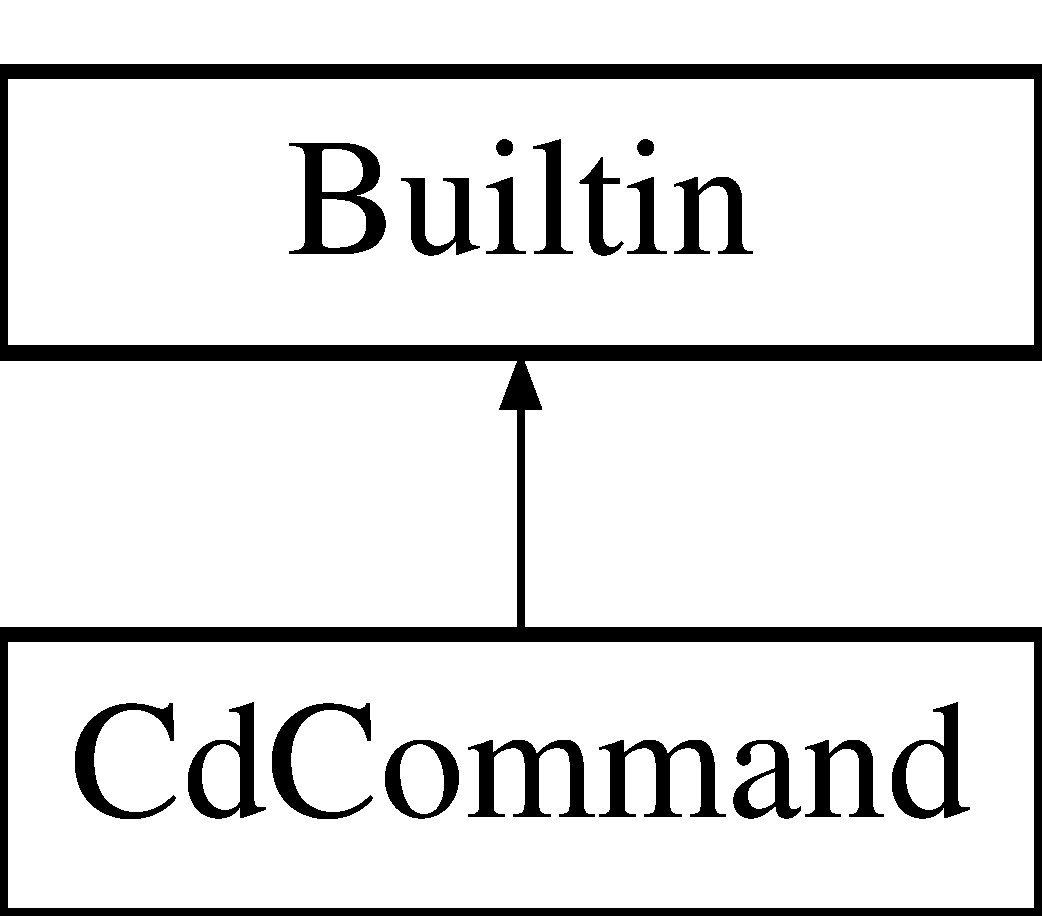
\includegraphics[height=2.000000cm]{classCdCommand}
\end{center}
\end{figure}


\subsection{Detailed Description}
Classe que implementa o comando cd. Sintaxe: cd $<$diretorio$>$ 

The documentation for this class was generated from the following files:\begin{DoxyCompactItemize}
\item 
\hyperlink{Builtin_8hpp}{Builtin.hpp}\item 
\hyperlink{Builtin_8cpp}{Builtin.cpp}\end{DoxyCompactItemize}

\hypertarget{classCommand}{
\section{Command Class Reference}
\label{classCommand}\index{Command@{Command}}
}


Representa um comando entrado pelo usuario. O comando representa tudo que esta numa linha ou antes de um \&.  




{\ttfamily \#include $<$Command.hpp$>$}

\subsection*{Public Member Functions}
\begin{DoxyCompactItemize}
\item 
\hyperlink{classCommand_a649b404d34720e098d6e0de6b07ad0c1}{Command} (std::vector$<$ std::string $>$ \&parameters, std::string in=std::string(), std::string out=std::string(), std::string err=std::string(), bool outAppend=false, bool errAppend=false)
\item 
\hyperlink{classCommand_ab552bb3a07fdd1acbfd8ea76e69b2278}{$\sim$Command} ()
\item 
std::string \hyperlink{classCommand_a660ad6733da715bcd5f74a38c04f4527}{getIn} ()
\item 
std::string \hyperlink{classCommand_a63ab07191770dd7f8133e49f8c4552d6}{getOut} ()
\item 
std::string \hyperlink{classCommand_a0421ff1ec0e2aec12fe8a334ceaea3ef}{getErr} ()
\item 
bool \hyperlink{classCommand_a054da0acd3b09e33c40df6865fc29c55}{getOutAppend} ()
\item 
bool \hyperlink{classCommand_a59a9ec8f011e3467e36ad72a8bcd3129}{getErrAppend} ()
\item 
const char $\ast$$\ast$ \hyperlink{classCommand_a37ef9c4ef69e9de78c138b0fe6b98f9f}{getExecv} ()
\end{DoxyCompactItemize}


\subsection{Detailed Description}
Representa um comando entrado pelo usuario. O comando representa tudo que esta numa linha ou antes de um \&. 

\subsection{Constructor \& Destructor Documentation}
\hypertarget{classCommand_a649b404d34720e098d6e0de6b07ad0c1}{
\index{Command@{Command}!Command@{Command}}
\index{Command@{Command}!Command@{Command}}
\subsubsection[{Command}]{\setlength{\rightskip}{0pt plus 5cm}Command::Command (
\begin{DoxyParamCaption}
\item[{std::vector$<$ std::string $>$ \&}]{parameters, }
\item[{std::string}]{in = {\ttfamily std::string()}, }
\item[{std::string}]{out = {\ttfamily std::string()}, }
\item[{std::string}]{err = {\ttfamily std::string()}, }
\item[{bool}]{outAppend = {\ttfamily false}, }
\item[{bool}]{errAppend = {\ttfamily false}}
\end{DoxyParamCaption}
)}}
\label{classCommand_a649b404d34720e098d6e0de6b07ad0c1}

\begin{DoxyParams}{Parameters}
{\em parameters} & Parametros utilizados na chamada do comando. \\
\hline
{\em in} & Nome do aquivo de redirecionamento de entrada \\
\hline
{\em out} & Nome do aquivo de redirecionamento de saida. \\
\hline
{\em err} & Nome do aquivo de redirecionamento de erro. \\
\hline
{\em outAppend} & Se o redirecionamento de saida concatenara com o arquivo ja existente. \\
\hline
{\em errAppend} & Se o redirecionamento de erro concatenara com o arquivo ja existente. \\
\hline
\end{DoxyParams}
\hypertarget{classCommand_ab552bb3a07fdd1acbfd8ea76e69b2278}{
\index{Command@{Command}!$\sim$Command@{$\sim$Command}}
\index{$\sim$Command@{$\sim$Command}!Command@{Command}}
\subsubsection[{$\sim$Command}]{\setlength{\rightskip}{0pt plus 5cm}Command::$\sim$Command (
\begin{DoxyParamCaption}
{}
\end{DoxyParamCaption}
)}}
\label{classCommand_ab552bb3a07fdd1acbfd8ea76e69b2278}


\subsection{Member Function Documentation}
\hypertarget{classCommand_a0421ff1ec0e2aec12fe8a334ceaea3ef}{
\index{Command@{Command}!getErr@{getErr}}
\index{getErr@{getErr}!Command@{Command}}
\subsubsection[{getErr}]{\setlength{\rightskip}{0pt plus 5cm}std::string Command::getErr (
\begin{DoxyParamCaption}
{}
\end{DoxyParamCaption}
)}}
\label{classCommand_a0421ff1ec0e2aec12fe8a334ceaea3ef}
\begin{DoxyReturn}{Returns}
Nome do arquivo de redirecionamento de erro. 
\end{DoxyReturn}
\hypertarget{classCommand_a59a9ec8f011e3467e36ad72a8bcd3129}{
\index{Command@{Command}!getErrAppend@{getErrAppend}}
\index{getErrAppend@{getErrAppend}!Command@{Command}}
\subsubsection[{getErrAppend}]{\setlength{\rightskip}{0pt plus 5cm}bool Command::getErrAppend (
\begin{DoxyParamCaption}
{}
\end{DoxyParamCaption}
)}}
\label{classCommand_a59a9ec8f011e3467e36ad72a8bcd3129}
\begin{DoxyReturn}{Returns}
Se deve haver anexacao no arquivo de erro. 
\end{DoxyReturn}
\hypertarget{classCommand_a37ef9c4ef69e9de78c138b0fe6b98f9f}{
\index{Command@{Command}!getExecv@{getExecv}}
\index{getExecv@{getExecv}!Command@{Command}}
\subsubsection[{getExecv}]{\setlength{\rightskip}{0pt plus 5cm}const char $\ast$$\ast$ Command::getExecv (
\begin{DoxyParamCaption}
{}
\end{DoxyParamCaption}
)}}
\label{classCommand_a37ef9c4ef69e9de78c138b0fe6b98f9f}
\hypertarget{classCommand_a660ad6733da715bcd5f74a38c04f4527}{
\index{Command@{Command}!getIn@{getIn}}
\index{getIn@{getIn}!Command@{Command}}
\subsubsection[{getIn}]{\setlength{\rightskip}{0pt plus 5cm}std::string Command::getIn (
\begin{DoxyParamCaption}
{}
\end{DoxyParamCaption}
)}}
\label{classCommand_a660ad6733da715bcd5f74a38c04f4527}
\begin{DoxyReturn}{Returns}
Nome do arquivo de redirecionamento de entrada. 
\end{DoxyReturn}
\hypertarget{classCommand_a63ab07191770dd7f8133e49f8c4552d6}{
\index{Command@{Command}!getOut@{getOut}}
\index{getOut@{getOut}!Command@{Command}}
\subsubsection[{getOut}]{\setlength{\rightskip}{0pt plus 5cm}std::string Command::getOut (
\begin{DoxyParamCaption}
{}
\end{DoxyParamCaption}
)}}
\label{classCommand_a63ab07191770dd7f8133e49f8c4552d6}
\begin{DoxyReturn}{Returns}
Nome do arquivo de redirecionamento de saida. 
\end{DoxyReturn}
\hypertarget{classCommand_a054da0acd3b09e33c40df6865fc29c55}{
\index{Command@{Command}!getOutAppend@{getOutAppend}}
\index{getOutAppend@{getOutAppend}!Command@{Command}}
\subsubsection[{getOutAppend}]{\setlength{\rightskip}{0pt plus 5cm}bool Command::getOutAppend (
\begin{DoxyParamCaption}
{}
\end{DoxyParamCaption}
)}}
\label{classCommand_a054da0acd3b09e33c40df6865fc29c55}
\begin{DoxyReturn}{Returns}
Se deve haver anexacao no arquivo de saida. 
\end{DoxyReturn}


The documentation for this class was generated from the following files:\begin{DoxyCompactItemize}
\item 
\hyperlink{Command_8hpp}{Command.hpp}\item 
\hyperlink{Command_8cpp}{Command.cpp}\end{DoxyCompactItemize}

\hypertarget{classCommandLine}{
\section{CommandLine Class Reference}
\label{classCommandLine}\index{CommandLine@{CommandLine}}
}


Represeta uma linha de comando.  




{\ttfamily \#include $<$CommandLine.hpp$>$}

\subsection*{Public Member Functions}
\begin{DoxyCompactItemize}
\item 
\hyperlink{classCommandLine}{CommandLine} \& \hyperlink{classCommandLine_a6afe6535f161927c0f658c51b9b63387}{operator=} (\hyperlink{classCommandLine}{CommandLine} \&commandLine)
\item 
\hyperlink{classCommandLine_a5c92f3c1c27926725eba68012f94d037}{CommandLine} (std::list$<$ \hyperlink{classCommand}{Command} $\ast$ $>$ $\ast$pipeline, bool background)
\begin{DoxyCompactList}\small\item\em Construtor. \item\end{DoxyCompactList}\item 
\hyperlink{classCommandLine_ac359efccafe57f845b1f747a9db3c6d9}{$\sim$CommandLine} ()
\item 
\hyperlink{classCommand}{Command} $\ast$ \hyperlink{classCommandLine_a34c3031124c1716e37170c5e60b487b2}{next} ()
\begin{DoxyCompactList}\small\item\em Navega pela pipeline existente A cada utilizacao, o comando extraido e retirado completamente da pipeline existente. \item\end{DoxyCompactList}\item 
bool \hyperlink{classCommandLine_a1994cb40c62ba84af078662842009a0b}{hasNext} ()
\item 
bool \hyperlink{classCommandLine_a4dfa18cb1625e1d25c6e5e68bbbc712e}{isBackground} ()
\end{DoxyCompactItemize}


\subsection{Detailed Description}
Represeta uma linha de comando. Uma linha de comando pode conter uma serie de comandos em pipeline e termina quando ha um \& ou um final de linha. A linha de comando pode ser gerada por uma instancia de \hyperlink{classParser}{Parser}

\begin{DoxySeeAlso}{See also}
\hyperlink{classCommand}{Command}, \hyperlink{classParser}{Parser} 
\end{DoxySeeAlso}


\subsection{Constructor \& Destructor Documentation}
\hypertarget{classCommandLine_a5c92f3c1c27926725eba68012f94d037}{
\index{CommandLine@{CommandLine}!CommandLine@{CommandLine}}
\index{CommandLine@{CommandLine}!CommandLine@{CommandLine}}
\subsubsection[{CommandLine}]{\setlength{\rightskip}{0pt plus 5cm}CommandLine::CommandLine (
\begin{DoxyParamCaption}
\item[{std::list$<$ {\bf Command} $\ast$ $>$ $\ast$}]{pipeline, }
\item[{bool}]{background}
\end{DoxyParamCaption}
)}}
\label{classCommandLine_a5c92f3c1c27926725eba68012f94d037}


Construtor. 


\begin{DoxyParams}{Parameters}
{\em pipeLine} & lista de comandos representando a pipeline \\
\hline
{\em background} & verdadeira, caso a pipeline deva ser executada em segundo plano \\
\hline
\end{DoxyParams}
\hypertarget{classCommandLine_ac359efccafe57f845b1f747a9db3c6d9}{
\index{CommandLine@{CommandLine}!$\sim$CommandLine@{$\sim$CommandLine}}
\index{$\sim$CommandLine@{$\sim$CommandLine}!CommandLine@{CommandLine}}
\subsubsection[{$\sim$CommandLine}]{\setlength{\rightskip}{0pt plus 5cm}CommandLine::$\sim$CommandLine (
\begin{DoxyParamCaption}
{}
\end{DoxyParamCaption}
)}}
\label{classCommandLine_ac359efccafe57f845b1f747a9db3c6d9}


\subsection{Member Function Documentation}
\hypertarget{classCommandLine_a1994cb40c62ba84af078662842009a0b}{
\index{CommandLine@{CommandLine}!hasNext@{hasNext}}
\index{hasNext@{hasNext}!CommandLine@{CommandLine}}
\subsubsection[{hasNext}]{\setlength{\rightskip}{0pt plus 5cm}bool CommandLine::hasNext (
\begin{DoxyParamCaption}
{}
\end{DoxyParamCaption}
)}}
\label{classCommandLine_a1994cb40c62ba84af078662842009a0b}
\begin{DoxyReturn}{Returns}
Verdadeiro se a pipeline nao esta vazia 
\end{DoxyReturn}
\hypertarget{classCommandLine_a4dfa18cb1625e1d25c6e5e68bbbc712e}{
\index{CommandLine@{CommandLine}!isBackground@{isBackground}}
\index{isBackground@{isBackground}!CommandLine@{CommandLine}}
\subsubsection[{isBackground}]{\setlength{\rightskip}{0pt plus 5cm}bool CommandLine::isBackground (
\begin{DoxyParamCaption}
{}
\end{DoxyParamCaption}
)}}
\label{classCommandLine_a4dfa18cb1625e1d25c6e5e68bbbc712e}
\begin{DoxyReturn}{Returns}
Verdadeiro se a pipeline deve ser executada em segundo plano 
\end{DoxyReturn}
\hypertarget{classCommandLine_a34c3031124c1716e37170c5e60b487b2}{
\index{CommandLine@{CommandLine}!next@{next}}
\index{next@{next}!CommandLine@{CommandLine}}
\subsubsection[{next}]{\setlength{\rightskip}{0pt plus 5cm}{\bf Command} $\ast$ CommandLine::next (
\begin{DoxyParamCaption}
{}
\end{DoxyParamCaption}
)}}
\label{classCommandLine_a34c3031124c1716e37170c5e60b487b2}


Navega pela pipeline existente A cada utilizacao, o comando extraido e retirado completamente da pipeline existente. 

\begin{DoxyReturn}{Returns}
Um ponteiro para o proximo comando da pipeline existente ou NULL o ultimo comando retirado tenha sido o ultimo 
\end{DoxyReturn}
\hypertarget{classCommandLine_a6afe6535f161927c0f658c51b9b63387}{
\index{CommandLine@{CommandLine}!operator=@{operator=}}
\index{operator=@{operator=}!CommandLine@{CommandLine}}
\subsubsection[{operator=}]{\setlength{\rightskip}{0pt plus 5cm}{\bf CommandLine}\& CommandLine::operator= (
\begin{DoxyParamCaption}
\item[{{\bf CommandLine} \&}]{commandLine}
\end{DoxyParamCaption}
)}}
\label{classCommandLine_a6afe6535f161927c0f658c51b9b63387}


The documentation for this class was generated from the following files:\begin{DoxyCompactItemize}
\item 
\hyperlink{CommandLine_8hpp}{CommandLine.hpp}\item 
\hyperlink{CommandLine_8cpp}{CommandLine.cpp}\end{DoxyCompactItemize}

\hypertarget{classgprof2dot_1_1Cycle}{
\section{gprof2dot::Cycle Class Reference}
\label{classgprof2dot_1_1Cycle}\index{gprof2dot::Cycle@{gprof2dot::Cycle}}
}
Inheritance diagram for gprof2dot::Cycle:\begin{figure}[H]
\begin{center}
\leavevmode
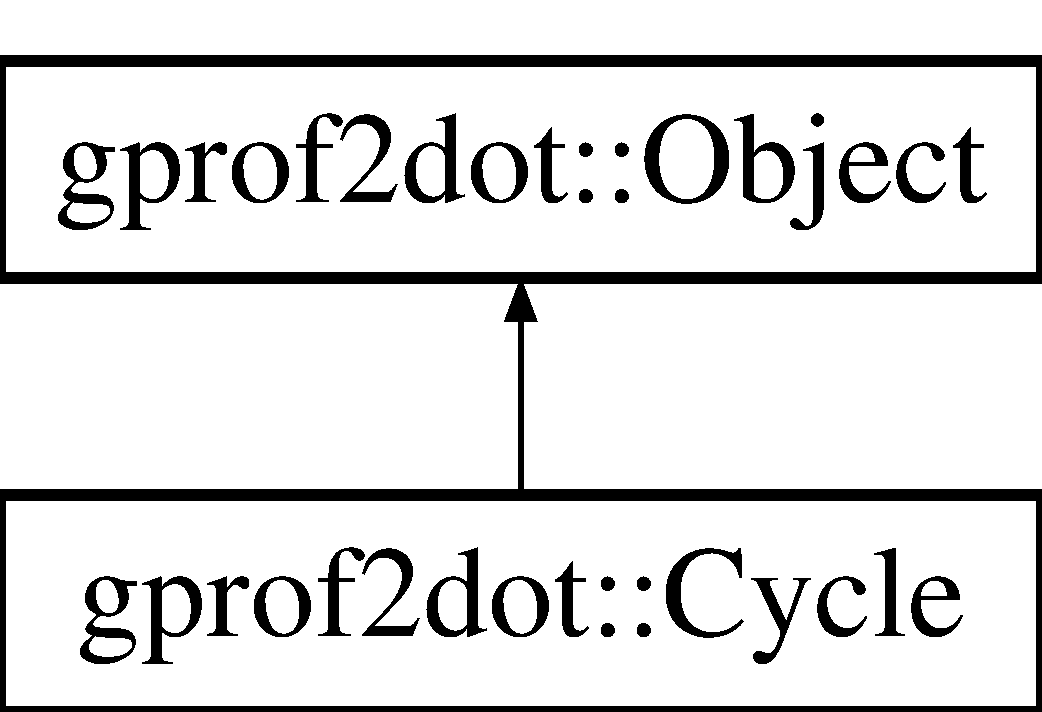
\includegraphics[height=2.000000cm]{classgprof2dot_1_1Cycle}
\end{center}
\end{figure}
\subsection*{Public Member Functions}
\begin{DoxyCompactItemize}
\item 
def \hyperlink{classgprof2dot_1_1Cycle_affb987dd26a328ded48d43e4acd9cdef}{\_\-\_\-init\_\-\_\-}
\item 
def \hyperlink{classgprof2dot_1_1Cycle_a593b54837816e005b45b874b65bfb507}{add\_\-function}
\end{DoxyCompactItemize}
\subsection*{Public Attributes}
\begin{DoxyCompactItemize}
\item 
\hyperlink{classgprof2dot_1_1Cycle_aabc895dbfe6d085881b008b2ae77d74c}{functions}
\end{DoxyCompactItemize}


\subsection{Detailed Description}
\begin{DoxyVerb}A cycle made from recursive function calls.\end{DoxyVerb}
 

\subsection{Constructor \& Destructor Documentation}
\hypertarget{classgprof2dot_1_1Cycle_affb987dd26a328ded48d43e4acd9cdef}{
\index{gprof2dot::Cycle@{gprof2dot::Cycle}!\_\-\_\-init\_\-\_\-@{\_\-\_\-init\_\-\_\-}}
\index{\_\-\_\-init\_\-\_\-@{\_\-\_\-init\_\-\_\-}!gprof2dot::Cycle@{gprof2dot::Cycle}}
\subsubsection[{\_\-\_\-init\_\-\_\-}]{\setlength{\rightskip}{0pt plus 5cm}def gprof2dot::Cycle::\_\-\_\-init\_\-\_\- (
\begin{DoxyParamCaption}
\item[{}]{self}
\end{DoxyParamCaption}
)}}
\label{classgprof2dot_1_1Cycle_affb987dd26a328ded48d43e4acd9cdef}


\subsection{Member Function Documentation}
\hypertarget{classgprof2dot_1_1Cycle_a593b54837816e005b45b874b65bfb507}{
\index{gprof2dot::Cycle@{gprof2dot::Cycle}!add\_\-function@{add\_\-function}}
\index{add\_\-function@{add\_\-function}!gprof2dot::Cycle@{gprof2dot::Cycle}}
\subsubsection[{add\_\-function}]{\setlength{\rightskip}{0pt plus 5cm}def gprof2dot::Cycle::add\_\-function (
\begin{DoxyParamCaption}
\item[{}]{self, }
\item[{}]{function}
\end{DoxyParamCaption}
)}}
\label{classgprof2dot_1_1Cycle_a593b54837816e005b45b874b65bfb507}


\subsection{Member Data Documentation}
\hypertarget{classgprof2dot_1_1Cycle_aabc895dbfe6d085881b008b2ae77d74c}{
\index{gprof2dot::Cycle@{gprof2dot::Cycle}!functions@{functions}}
\index{functions@{functions}!gprof2dot::Cycle@{gprof2dot::Cycle}}
\subsubsection[{functions}]{\setlength{\rightskip}{0pt plus 5cm}{\bf gprof2dot::Cycle::functions}}}
\label{classgprof2dot_1_1Cycle_aabc895dbfe6d085881b008b2ae77d74c}


The documentation for this class was generated from the following file:\begin{DoxyCompactItemize}
\item 
\hyperlink{gprof2dot_8py}{gprof2dot.py}\end{DoxyCompactItemize}

\hypertarget{classgprof2dot_1_1DotWriter}{
\section{gprof2dot::DotWriter Class Reference}
\label{classgprof2dot_1_1DotWriter}\index{gprof2dot::DotWriter@{gprof2dot::DotWriter}}
}
\subsection*{Public Member Functions}
\begin{DoxyCompactItemize}
\item 
def \hyperlink{classgprof2dot_1_1DotWriter_a56d86338edd95cc7c4018d3bc083d64a}{\_\-\_\-init\_\-\_\-}
\item 
def \hyperlink{classgprof2dot_1_1DotWriter_a4e91d75c9bac72b29be59956676c66de}{graph}
\item 
def \hyperlink{classgprof2dot_1_1DotWriter_a45451f875299bba49dcefb9bc53c298a}{begin\_\-graph}
\item 
def \hyperlink{classgprof2dot_1_1DotWriter_a74dc98f24aa019be858aa060586f6823}{end\_\-graph}
\item 
def \hyperlink{classgprof2dot_1_1DotWriter_a1ffd72f8933e8c278ba235cd8f2fba1a}{attr}
\item 
def \hyperlink{classgprof2dot_1_1DotWriter_af42321fbb48851c5fbd01b7dc7e0b810}{node}
\item 
def \hyperlink{classgprof2dot_1_1DotWriter_a26bc5afdf3921b3b6b5df9a0a9309de5}{edge}
\item 
def \hyperlink{classgprof2dot_1_1DotWriter_a5b16841885002ef23c1a5140719e3984}{attr\_\-list}
\item 
def \hyperlink{classgprof2dot_1_1DotWriter_afbea6f6f87496d4babd43853a97f5582}{id}
\item 
def \hyperlink{classgprof2dot_1_1DotWriter_ab2ca20eced759774a87874a4d6df748d}{color}
\item 
def \hyperlink{classgprof2dot_1_1DotWriter_ad71838639495e6f834fd01657dcaff41}{escape}
\item 
def \hyperlink{classgprof2dot_1_1DotWriter_a9746c83e8b3bed4537d408fb92595e24}{write}
\end{DoxyCompactItemize}
\subsection*{Public Attributes}
\begin{DoxyCompactItemize}
\item 
\hyperlink{classgprof2dot_1_1DotWriter_a266d8247c93fdd14af35568d52411253}{fp}
\end{DoxyCompactItemize}


\subsection{Detailed Description}
\begin{DoxyVerb}Writer for the DOT language.

See also:
- "The DOT Language" specification
  http://www.graphviz.org/doc/info/lang.html
\end{DoxyVerb}
 

\subsection{Constructor \& Destructor Documentation}
\hypertarget{classgprof2dot_1_1DotWriter_a56d86338edd95cc7c4018d3bc083d64a}{
\index{gprof2dot::DotWriter@{gprof2dot::DotWriter}!\_\-\_\-init\_\-\_\-@{\_\-\_\-init\_\-\_\-}}
\index{\_\-\_\-init\_\-\_\-@{\_\-\_\-init\_\-\_\-}!gprof2dot::DotWriter@{gprof2dot::DotWriter}}
\subsubsection[{\_\-\_\-init\_\-\_\-}]{\setlength{\rightskip}{0pt plus 5cm}def gprof2dot::DotWriter::\_\-\_\-init\_\-\_\- (
\begin{DoxyParamCaption}
\item[{}]{self, }
\item[{}]{fp}
\end{DoxyParamCaption}
)}}
\label{classgprof2dot_1_1DotWriter_a56d86338edd95cc7c4018d3bc083d64a}


\subsection{Member Function Documentation}
\hypertarget{classgprof2dot_1_1DotWriter_a1ffd72f8933e8c278ba235cd8f2fba1a}{
\index{gprof2dot::DotWriter@{gprof2dot::DotWriter}!attr@{attr}}
\index{attr@{attr}!gprof2dot::DotWriter@{gprof2dot::DotWriter}}
\subsubsection[{attr}]{\setlength{\rightskip}{0pt plus 5cm}def gprof2dot::DotWriter::attr (
\begin{DoxyParamCaption}
\item[{}]{self, }
\item[{}]{what, }
\item[{}]{attrs}
\end{DoxyParamCaption}
)}}
\label{classgprof2dot_1_1DotWriter_a1ffd72f8933e8c278ba235cd8f2fba1a}
\hypertarget{classgprof2dot_1_1DotWriter_a5b16841885002ef23c1a5140719e3984}{
\index{gprof2dot::DotWriter@{gprof2dot::DotWriter}!attr\_\-list@{attr\_\-list}}
\index{attr\_\-list@{attr\_\-list}!gprof2dot::DotWriter@{gprof2dot::DotWriter}}
\subsubsection[{attr\_\-list}]{\setlength{\rightskip}{0pt plus 5cm}def gprof2dot::DotWriter::attr\_\-list (
\begin{DoxyParamCaption}
\item[{}]{self, }
\item[{}]{attrs}
\end{DoxyParamCaption}
)}}
\label{classgprof2dot_1_1DotWriter_a5b16841885002ef23c1a5140719e3984}
\hypertarget{classgprof2dot_1_1DotWriter_a45451f875299bba49dcefb9bc53c298a}{
\index{gprof2dot::DotWriter@{gprof2dot::DotWriter}!begin\_\-graph@{begin\_\-graph}}
\index{begin\_\-graph@{begin\_\-graph}!gprof2dot::DotWriter@{gprof2dot::DotWriter}}
\subsubsection[{begin\_\-graph}]{\setlength{\rightskip}{0pt plus 5cm}def gprof2dot::DotWriter::begin\_\-graph (
\begin{DoxyParamCaption}
\item[{}]{self}
\end{DoxyParamCaption}
)}}
\label{classgprof2dot_1_1DotWriter_a45451f875299bba49dcefb9bc53c298a}
\hypertarget{classgprof2dot_1_1DotWriter_ab2ca20eced759774a87874a4d6df748d}{
\index{gprof2dot::DotWriter@{gprof2dot::DotWriter}!color@{color}}
\index{color@{color}!gprof2dot::DotWriter@{gprof2dot::DotWriter}}
\subsubsection[{color}]{\setlength{\rightskip}{0pt plus 5cm}def gprof2dot::DotWriter::color (
\begin{DoxyParamCaption}
\item[{}]{self, }
\item[{}]{r, }
\item[{}]{g, }
\item[{}]{b}
\end{DoxyParamCaption}
)}}
\label{classgprof2dot_1_1DotWriter_ab2ca20eced759774a87874a4d6df748d}
\hypertarget{classgprof2dot_1_1DotWriter_a26bc5afdf3921b3b6b5df9a0a9309de5}{
\index{gprof2dot::DotWriter@{gprof2dot::DotWriter}!edge@{edge}}
\index{edge@{edge}!gprof2dot::DotWriter@{gprof2dot::DotWriter}}
\subsubsection[{edge}]{\setlength{\rightskip}{0pt plus 5cm}def gprof2dot::DotWriter::edge (
\begin{DoxyParamCaption}
\item[{}]{self, }
\item[{}]{src, }
\item[{}]{dst, }
\item[{}]{attrs}
\end{DoxyParamCaption}
)}}
\label{classgprof2dot_1_1DotWriter_a26bc5afdf3921b3b6b5df9a0a9309de5}
\hypertarget{classgprof2dot_1_1DotWriter_a74dc98f24aa019be858aa060586f6823}{
\index{gprof2dot::DotWriter@{gprof2dot::DotWriter}!end\_\-graph@{end\_\-graph}}
\index{end\_\-graph@{end\_\-graph}!gprof2dot::DotWriter@{gprof2dot::DotWriter}}
\subsubsection[{end\_\-graph}]{\setlength{\rightskip}{0pt plus 5cm}def gprof2dot::DotWriter::end\_\-graph (
\begin{DoxyParamCaption}
\item[{}]{self}
\end{DoxyParamCaption}
)}}
\label{classgprof2dot_1_1DotWriter_a74dc98f24aa019be858aa060586f6823}
\hypertarget{classgprof2dot_1_1DotWriter_ad71838639495e6f834fd01657dcaff41}{
\index{gprof2dot::DotWriter@{gprof2dot::DotWriter}!escape@{escape}}
\index{escape@{escape}!gprof2dot::DotWriter@{gprof2dot::DotWriter}}
\subsubsection[{escape}]{\setlength{\rightskip}{0pt plus 5cm}def gprof2dot::DotWriter::escape (
\begin{DoxyParamCaption}
\item[{}]{self, }
\item[{}]{s}
\end{DoxyParamCaption}
)}}
\label{classgprof2dot_1_1DotWriter_ad71838639495e6f834fd01657dcaff41}
\hypertarget{classgprof2dot_1_1DotWriter_a4e91d75c9bac72b29be59956676c66de}{
\index{gprof2dot::DotWriter@{gprof2dot::DotWriter}!graph@{graph}}
\index{graph@{graph}!gprof2dot::DotWriter@{gprof2dot::DotWriter}}
\subsubsection[{graph}]{\setlength{\rightskip}{0pt plus 5cm}def gprof2dot::DotWriter::graph (
\begin{DoxyParamCaption}
\item[{}]{self, }
\item[{}]{profile, }
\item[{}]{theme}
\end{DoxyParamCaption}
)}}
\label{classgprof2dot_1_1DotWriter_a4e91d75c9bac72b29be59956676c66de}
\hypertarget{classgprof2dot_1_1DotWriter_afbea6f6f87496d4babd43853a97f5582}{
\index{gprof2dot::DotWriter@{gprof2dot::DotWriter}!id@{id}}
\index{id@{id}!gprof2dot::DotWriter@{gprof2dot::DotWriter}}
\subsubsection[{id}]{\setlength{\rightskip}{0pt plus 5cm}def gprof2dot::DotWriter::id (
\begin{DoxyParamCaption}
\item[{}]{self, }
\item[{}]{id}
\end{DoxyParamCaption}
)}}
\label{classgprof2dot_1_1DotWriter_afbea6f6f87496d4babd43853a97f5582}
\hypertarget{classgprof2dot_1_1DotWriter_af42321fbb48851c5fbd01b7dc7e0b810}{
\index{gprof2dot::DotWriter@{gprof2dot::DotWriter}!node@{node}}
\index{node@{node}!gprof2dot::DotWriter@{gprof2dot::DotWriter}}
\subsubsection[{node}]{\setlength{\rightskip}{0pt plus 5cm}def gprof2dot::DotWriter::node (
\begin{DoxyParamCaption}
\item[{}]{self, }
\item[{}]{node, }
\item[{}]{attrs}
\end{DoxyParamCaption}
)}}
\label{classgprof2dot_1_1DotWriter_af42321fbb48851c5fbd01b7dc7e0b810}
\hypertarget{classgprof2dot_1_1DotWriter_a9746c83e8b3bed4537d408fb92595e24}{
\index{gprof2dot::DotWriter@{gprof2dot::DotWriter}!write@{write}}
\index{write@{write}!gprof2dot::DotWriter@{gprof2dot::DotWriter}}
\subsubsection[{write}]{\setlength{\rightskip}{0pt plus 5cm}def gprof2dot::DotWriter::write (
\begin{DoxyParamCaption}
\item[{}]{self, }
\item[{}]{s}
\end{DoxyParamCaption}
)}}
\label{classgprof2dot_1_1DotWriter_a9746c83e8b3bed4537d408fb92595e24}


\subsection{Member Data Documentation}
\hypertarget{classgprof2dot_1_1DotWriter_a266d8247c93fdd14af35568d52411253}{
\index{gprof2dot::DotWriter@{gprof2dot::DotWriter}!fp@{fp}}
\index{fp@{fp}!gprof2dot::DotWriter@{gprof2dot::DotWriter}}
\subsubsection[{fp}]{\setlength{\rightskip}{0pt plus 5cm}{\bf gprof2dot::DotWriter::fp}}}
\label{classgprof2dot_1_1DotWriter_a266d8247c93fdd14af35568d52411253}


The documentation for this class was generated from the following file:\begin{DoxyCompactItemize}
\item 
\hyperlink{gprof2dot_8py}{gprof2dot.py}\end{DoxyCompactItemize}

\hypertarget{classgprof2dot_1_1Event}{
\section{gprof2dot::Event Class Reference}
\label{classgprof2dot_1_1Event}\index{gprof2dot::Event@{gprof2dot::Event}}
}
\subsection*{Public Member Functions}
\begin{DoxyCompactItemize}
\item 
def \hyperlink{classgprof2dot_1_1Event_afa20b60008552a9204e4f03f0ee2ad6c}{\_\-\_\-init\_\-\_\-}
\item 
def \hyperlink{classgprof2dot_1_1Event_afddebbd653160481ff08fc7bf13d3cf2}{\_\-\_\-eq\_\-\_\-}
\item 
def \hyperlink{classgprof2dot_1_1Event_a66169db3de36baebd5d86d0cbcf21375}{\_\-\_\-hash\_\-\_\-}
\item 
def \hyperlink{classgprof2dot_1_1Event_acc16d016d072bc771eeda1a34997640f}{null}
\item 
def \hyperlink{classgprof2dot_1_1Event_afd3d6cb21db851048e9f59313fb189fe}{aggregate}
\item 
def \hyperlink{classgprof2dot_1_1Event_aeaeda65173fc69ffcc789351cadd30c3}{format}
\end{DoxyCompactItemize}
\subsection*{Public Attributes}
\begin{DoxyCompactItemize}
\item 
\hyperlink{classgprof2dot_1_1Event_ab50107b4654bfae38cd0c6de3a66a53b}{name}
\end{DoxyCompactItemize}


\subsection{Detailed Description}
\begin{DoxyVerb}Describe a kind of event, and its basic operations.\end{DoxyVerb}
 

\subsection{Constructor \& Destructor Documentation}
\hypertarget{classgprof2dot_1_1Event_afa20b60008552a9204e4f03f0ee2ad6c}{
\index{gprof2dot::Event@{gprof2dot::Event}!\_\-\_\-init\_\-\_\-@{\_\-\_\-init\_\-\_\-}}
\index{\_\-\_\-init\_\-\_\-@{\_\-\_\-init\_\-\_\-}!gprof2dot::Event@{gprof2dot::Event}}
\subsubsection[{\_\-\_\-init\_\-\_\-}]{\setlength{\rightskip}{0pt plus 5cm}def gprof2dot::Event::\_\-\_\-init\_\-\_\- (
\begin{DoxyParamCaption}
\item[{}]{self, }
\item[{}]{name, }
\item[{}]{null, }
\item[{}]{aggregator, }
\item[{}]{formatter = {\ttfamily str}}
\end{DoxyParamCaption}
)}}
\label{classgprof2dot_1_1Event_afa20b60008552a9204e4f03f0ee2ad6c}


\subsection{Member Function Documentation}
\hypertarget{classgprof2dot_1_1Event_afddebbd653160481ff08fc7bf13d3cf2}{
\index{gprof2dot::Event@{gprof2dot::Event}!\_\-\_\-eq\_\-\_\-@{\_\-\_\-eq\_\-\_\-}}
\index{\_\-\_\-eq\_\-\_\-@{\_\-\_\-eq\_\-\_\-}!gprof2dot::Event@{gprof2dot::Event}}
\subsubsection[{\_\-\_\-eq\_\-\_\-}]{\setlength{\rightskip}{0pt plus 5cm}def gprof2dot::Event::\_\-\_\-eq\_\-\_\- (
\begin{DoxyParamCaption}
\item[{}]{self, }
\item[{}]{other}
\end{DoxyParamCaption}
)}}
\label{classgprof2dot_1_1Event_afddebbd653160481ff08fc7bf13d3cf2}
\hypertarget{classgprof2dot_1_1Event_a66169db3de36baebd5d86d0cbcf21375}{
\index{gprof2dot::Event@{gprof2dot::Event}!\_\-\_\-hash\_\-\_\-@{\_\-\_\-hash\_\-\_\-}}
\index{\_\-\_\-hash\_\-\_\-@{\_\-\_\-hash\_\-\_\-}!gprof2dot::Event@{gprof2dot::Event}}
\subsubsection[{\_\-\_\-hash\_\-\_\-}]{\setlength{\rightskip}{0pt plus 5cm}def gprof2dot::Event::\_\-\_\-hash\_\-\_\- (
\begin{DoxyParamCaption}
\item[{}]{self}
\end{DoxyParamCaption}
)}}
\label{classgprof2dot_1_1Event_a66169db3de36baebd5d86d0cbcf21375}
\hypertarget{classgprof2dot_1_1Event_afd3d6cb21db851048e9f59313fb189fe}{
\index{gprof2dot::Event@{gprof2dot::Event}!aggregate@{aggregate}}
\index{aggregate@{aggregate}!gprof2dot::Event@{gprof2dot::Event}}
\subsubsection[{aggregate}]{\setlength{\rightskip}{0pt plus 5cm}def gprof2dot::Event::aggregate (
\begin{DoxyParamCaption}
\item[{}]{self, }
\item[{}]{val1, }
\item[{}]{val2}
\end{DoxyParamCaption}
)}}
\label{classgprof2dot_1_1Event_afd3d6cb21db851048e9f59313fb189fe}
\begin{DoxyVerb}Aggregate two event values.\end{DoxyVerb}
 \hypertarget{classgprof2dot_1_1Event_aeaeda65173fc69ffcc789351cadd30c3}{
\index{gprof2dot::Event@{gprof2dot::Event}!format@{format}}
\index{format@{format}!gprof2dot::Event@{gprof2dot::Event}}
\subsubsection[{format}]{\setlength{\rightskip}{0pt plus 5cm}def gprof2dot::Event::format (
\begin{DoxyParamCaption}
\item[{}]{self, }
\item[{}]{val}
\end{DoxyParamCaption}
)}}
\label{classgprof2dot_1_1Event_aeaeda65173fc69ffcc789351cadd30c3}
\begin{DoxyVerb}Format an event value.\end{DoxyVerb}
 \hypertarget{classgprof2dot_1_1Event_acc16d016d072bc771eeda1a34997640f}{
\index{gprof2dot::Event@{gprof2dot::Event}!null@{null}}
\index{null@{null}!gprof2dot::Event@{gprof2dot::Event}}
\subsubsection[{null}]{\setlength{\rightskip}{0pt plus 5cm}def gprof2dot::Event::null (
\begin{DoxyParamCaption}
\item[{}]{self}
\end{DoxyParamCaption}
)}}
\label{classgprof2dot_1_1Event_acc16d016d072bc771eeda1a34997640f}


\subsection{Member Data Documentation}
\hypertarget{classgprof2dot_1_1Event_ab50107b4654bfae38cd0c6de3a66a53b}{
\index{gprof2dot::Event@{gprof2dot::Event}!name@{name}}
\index{name@{name}!gprof2dot::Event@{gprof2dot::Event}}
\subsubsection[{name}]{\setlength{\rightskip}{0pt plus 5cm}{\bf gprof2dot::Event::name}}}
\label{classgprof2dot_1_1Event_ab50107b4654bfae38cd0c6de3a66a53b}


The documentation for this class was generated from the following file:\begin{DoxyCompactItemize}
\item 
\hyperlink{gprof2dot_8py}{gprof2dot.py}\end{DoxyCompactItemize}

\hypertarget{classExecutor}{
\section{Executor Class Reference}
\label{classExecutor}\index{Executor@{Executor}}
}


Responsavel pela execucao. Executa uma linha de comando.  




{\ttfamily \#include $<$Executor.hpp$>$}

\subsection*{Classes}
\begin{DoxyCompactItemize}
\item 
struct \hyperlink{structExecutor_1_1Job}{Job}
\end{DoxyCompactItemize}
\subsection*{Public Member Functions}
\begin{DoxyCompactItemize}
\item 
\hyperlink{classExecutor_af10e2be4ceafc43c65cb888d14a519de}{Executor} ()
\item 
void \hyperlink{classExecutor_ab0fe153cc70998a0b89837fab30c50c7}{run} (\hyperlink{classCommandLine}{CommandLine} $\ast$commandLine, std::map$<$ std::string, \hyperlink{classBuiltin}{Builtin} $\ast$ $>$ \&bCommands)
\begin{DoxyCompactList}\small\item\em Executa uma linha de comando. Executa os comandos de uma \hyperlink{classCommandLine}{CommandLine}. \item\end{DoxyCompactList}\item 
void \hyperlink{classExecutor_a62f3a102e3cd4fcfd66697e84bd6eb7a}{cleanUp} ()
\begin{DoxyCompactList}\small\item\em Realiza ajustes na lista de jobs, se necessario. Percorre a lista de jobs, removendo, atualizando status, quando necessario. \item\end{DoxyCompactList}\item 
void \hyperlink{classExecutor_aba6c22f3bd51d26d2fb403664294ada8}{setForeground} (int pid)
\begin{DoxyCompactList}\small\item\em Controle interno. Atualiza o job que esta em foreground. \item\end{DoxyCompactList}\item 
unsigned \hyperlink{classExecutor_a5f46c3263b42d9cbf043cc26351f75e0}{getLastForeground} ()
\item 
void \hyperlink{classExecutor_a29e399610629607f1f00cbb8f33eb3b3}{setLastForeground} (unsigned jobid)
\begin{DoxyCompactList}\small\item\em Altera qual processo deve ir para foreground. Quando ocorrer uma chamada a fg, o processo configurado sera utilizado. \item\end{DoxyCompactList}\item 
std::list$<$ \hyperlink{structExecutor_1_1Job}{Job} $>$ $\ast$ \hyperlink{classExecutor_a5514d88e0b4d4a04f8a3065a497af00e}{getJobs} ()
\end{DoxyCompactItemize}


\subsection{Detailed Description}
Responsavel pela execucao. Executa uma linha de comando. Uma instancia de \hyperlink{classExecutor}{Executor} guarda a lista de processos que sao extraidos das linhas de comando recebidas. Controla a atualizacao dos estados dos processos.

\begin{DoxySeeAlso}{See also}
\hyperlink{classCommandLine}{CommandLine}, \hyperlink{classCommand}{Command} 
\end{DoxySeeAlso}


\subsection{Constructor \& Destructor Documentation}
\hypertarget{classExecutor_af10e2be4ceafc43c65cb888d14a519de}{
\index{Executor@{Executor}!Executor@{Executor}}
\index{Executor@{Executor}!Executor@{Executor}}
\subsubsection[{Executor}]{\setlength{\rightskip}{0pt plus 5cm}Executor::Executor (
\begin{DoxyParamCaption}
{}
\end{DoxyParamCaption}
)}}
\label{classExecutor_af10e2be4ceafc43c65cb888d14a519de}


\subsection{Member Function Documentation}
\hypertarget{classExecutor_a62f3a102e3cd4fcfd66697e84bd6eb7a}{
\index{Executor@{Executor}!cleanUp@{cleanUp}}
\index{cleanUp@{cleanUp}!Executor@{Executor}}
\subsubsection[{cleanUp}]{\setlength{\rightskip}{0pt plus 5cm}void Executor::cleanUp (
\begin{DoxyParamCaption}
{}
\end{DoxyParamCaption}
)}}
\label{classExecutor_a62f3a102e3cd4fcfd66697e84bd6eb7a}


Realiza ajustes na lista de jobs, se necessario. Percorre a lista de jobs, removendo, atualizando status, quando necessario. 

\begin{DoxySeeAlso}{See also}
\hyperlink{structExecutor_1_1Job}{Job}, \hyperlink{namespacehandlers}{handlers} 
\end{DoxySeeAlso}
\hypertarget{classExecutor_a5514d88e0b4d4a04f8a3065a497af00e}{
\index{Executor@{Executor}!getJobs@{getJobs}}
\index{getJobs@{getJobs}!Executor@{Executor}}
\subsubsection[{getJobs}]{\setlength{\rightskip}{0pt plus 5cm}std::list$<$ {\bf Executor::Job} $>$ $\ast$ Executor::getJobs (
\begin{DoxyParamCaption}
{}
\end{DoxyParamCaption}
)}}
\label{classExecutor_a5514d88e0b4d4a04f8a3065a497af00e}
\begin{DoxyReturn}{Returns}
Ponteiro para a lista de jobs. 
\end{DoxyReturn}
\hypertarget{classExecutor_a5f46c3263b42d9cbf043cc26351f75e0}{
\index{Executor@{Executor}!getLastForeground@{getLastForeground}}
\index{getLastForeground@{getLastForeground}!Executor@{Executor}}
\subsubsection[{getLastForeground}]{\setlength{\rightskip}{0pt plus 5cm}unsigned Executor::getLastForeground (
\begin{DoxyParamCaption}
{}
\end{DoxyParamCaption}
)}}
\label{classExecutor_a5f46c3263b42d9cbf043cc26351f75e0}
\begin{DoxyReturn}{Returns}
JobID do processo que deve ir para foreground. 
\end{DoxyReturn}
\hypertarget{classExecutor_ab0fe153cc70998a0b89837fab30c50c7}{
\index{Executor@{Executor}!run@{run}}
\index{run@{run}!Executor@{Executor}}
\subsubsection[{run}]{\setlength{\rightskip}{0pt plus 5cm}void Executor::run (
\begin{DoxyParamCaption}
\item[{{\bf CommandLine} $\ast$}]{commandLine, }
\item[{std::map$<$ std::string, {\bf Builtin} $\ast$ $>$ \&}]{bCommands}
\end{DoxyParamCaption}
)}}
\label{classExecutor_ab0fe153cc70998a0b89837fab30c50c7}


Executa uma linha de comando. Executa os comandos de uma \hyperlink{classCommandLine}{CommandLine}. 

\begin{DoxySeeAlso}{See also}
\hyperlink{classParser}{Parser}, \hyperlink{classCommandLine}{CommandLine}, \hyperlink{classBuiltin}{Builtin} 
\end{DoxySeeAlso}

\begin{DoxyParams}{Parameters}
{\em commandLine} & Linha de comando a ser executada. \\
\hline
{\em bCommands} & Mapa que associa nomes de comandos internos a comandos internos. \\
\hline
\end{DoxyParams}
\hypertarget{classExecutor_aba6c22f3bd51d26d2fb403664294ada8}{
\index{Executor@{Executor}!setForeground@{setForeground}}
\index{setForeground@{setForeground}!Executor@{Executor}}
\subsubsection[{setForeground}]{\setlength{\rightskip}{0pt plus 5cm}void Executor::setForeground (
\begin{DoxyParamCaption}
\item[{int}]{pid}
\end{DoxyParamCaption}
)}}
\label{classExecutor_aba6c22f3bd51d26d2fb403664294ada8}


Controle interno. Atualiza o job que esta em foreground. 

\hypertarget{classExecutor_a29e399610629607f1f00cbb8f33eb3b3}{
\index{Executor@{Executor}!setLastForeground@{setLastForeground}}
\index{setLastForeground@{setLastForeground}!Executor@{Executor}}
\subsubsection[{setLastForeground}]{\setlength{\rightskip}{0pt plus 5cm}void Executor::setLastForeground (
\begin{DoxyParamCaption}
\item[{unsigned}]{jobid}
\end{DoxyParamCaption}
)}}
\label{classExecutor_a29e399610629607f1f00cbb8f33eb3b3}


Altera qual processo deve ir para foreground. Quando ocorrer uma chamada a fg, o processo configurado sera utilizado. 

\begin{DoxySeeAlso}{See also}
\hyperlink{classFgCommand}{FgCommand}, \hyperlink{classBgCommand}{BgCommand} 
\end{DoxySeeAlso}

\begin{DoxyParams}{Parameters}
{\em jobid} & JobID do processo a ser configurado. \\
\hline
\end{DoxyParams}


The documentation for this class was generated from the following files:\begin{DoxyCompactItemize}
\item 
\hyperlink{Executor_8hpp}{Executor.hpp}\item 
\hyperlink{Executor_8cpp}{Executor.cpp}\end{DoxyCompactItemize}

\hypertarget{classExitCommand}{
\section{ExitCommand Class Reference}
\label{classExitCommand}\index{ExitCommand@{ExitCommand}}
}


Classe que implementa o comando exit.  




{\ttfamily \#include $<$Builtin.hpp$>$}

Inheritance diagram for ExitCommand:\begin{figure}[H]
\begin{center}
\leavevmode
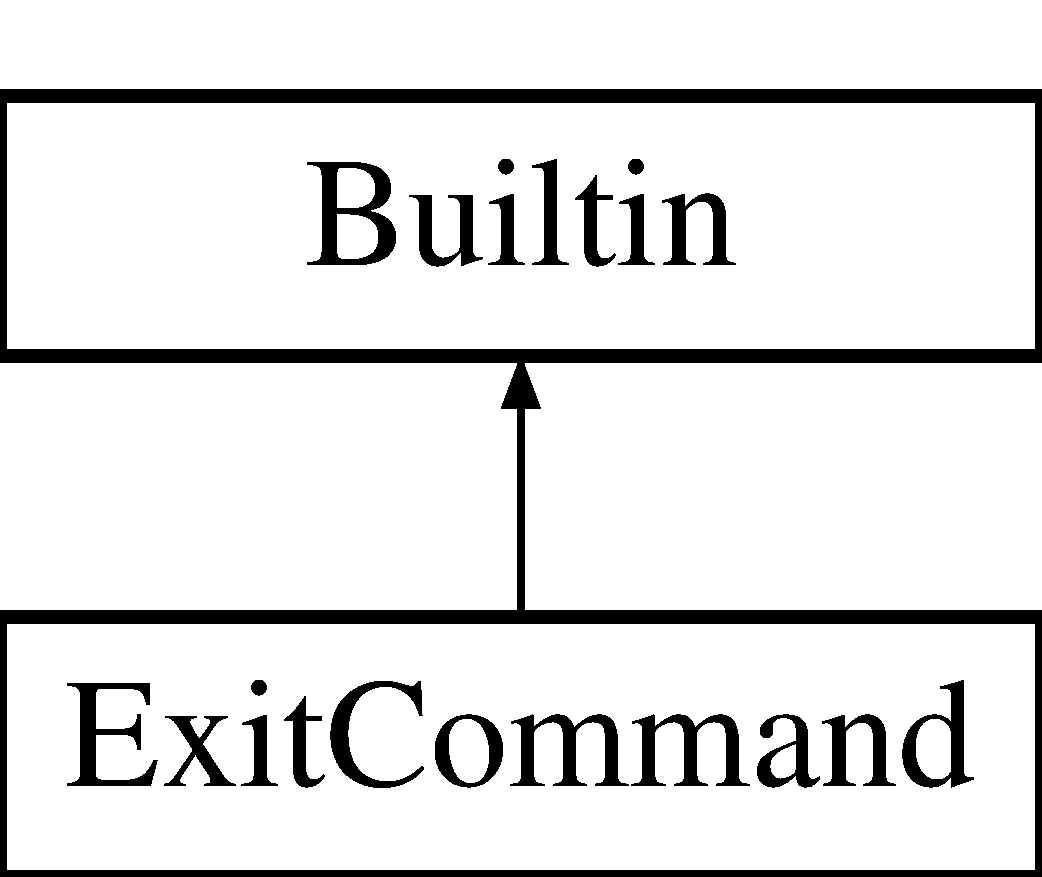
\includegraphics[height=2.000000cm]{classExitCommand}
\end{center}
\end{figure}


\subsection{Detailed Description}
Classe que implementa o comando exit. Sintaxe: exit, quit 

The documentation for this class was generated from the following files:\begin{DoxyCompactItemize}
\item 
\hyperlink{Builtin_8hpp}{Builtin.hpp}\item 
\hyperlink{Builtin_8cpp}{Builtin.cpp}\end{DoxyCompactItemize}

\hypertarget{classFgCommand}{
\section{FgCommand Class Reference}
\label{classFgCommand}\index{FgCommand@{FgCommand}}
}


{\ttfamily \#include $<$Builtin.hpp$>$}

Inheritance diagram for FgCommand:\begin{figure}[H]
\begin{center}
\leavevmode
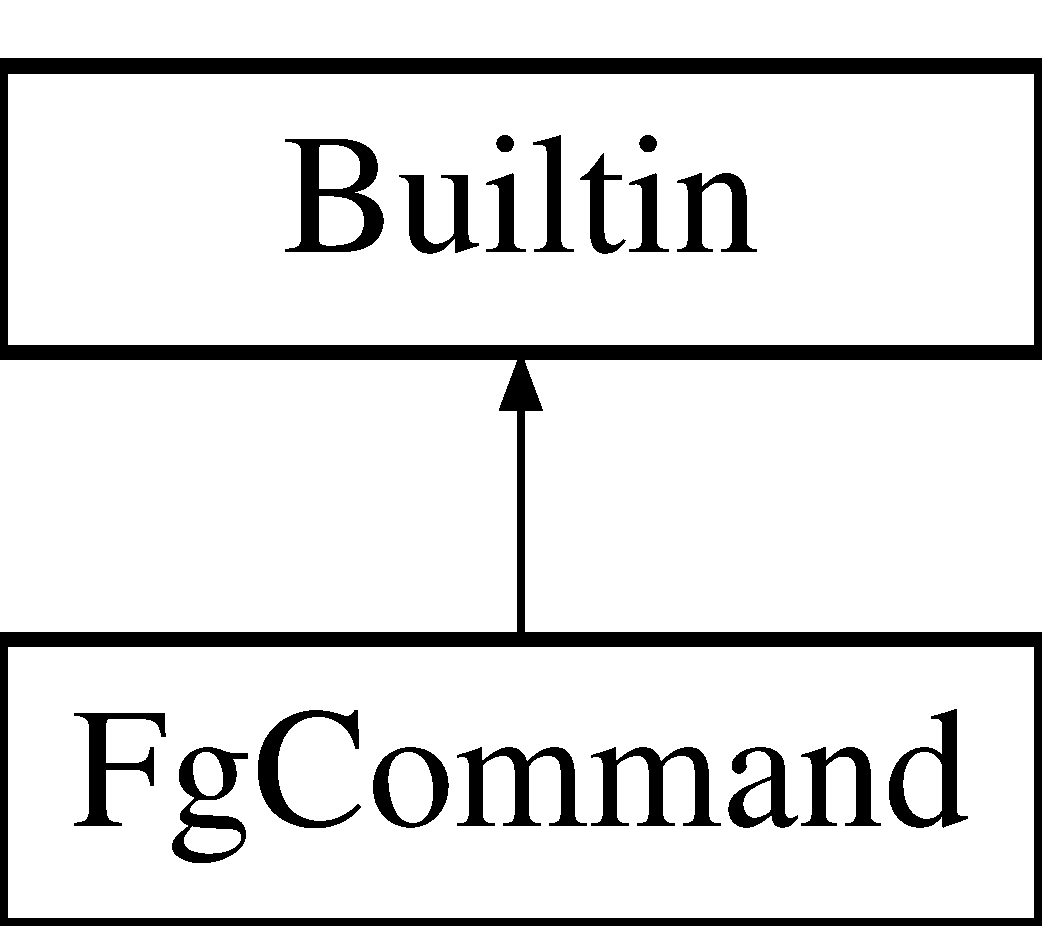
\includegraphics[height=2.000000cm]{classFgCommand}
\end{center}
\end{figure}


The documentation for this class was generated from the following files:\begin{DoxyCompactItemize}
\item 
\hyperlink{Builtin_8hpp}{Builtin.hpp}\item 
\hyperlink{Builtin_8cpp}{Builtin.cpp}\end{DoxyCompactItemize}

\hypertarget{classgprof2dot_1_1Function}{
\section{gprof2dot::Function Class Reference}
\label{classgprof2dot_1_1Function}\index{gprof2dot::Function@{gprof2dot::Function}}
}
Inheritance diagram for gprof2dot::Function:\begin{figure}[H]
\begin{center}
\leavevmode
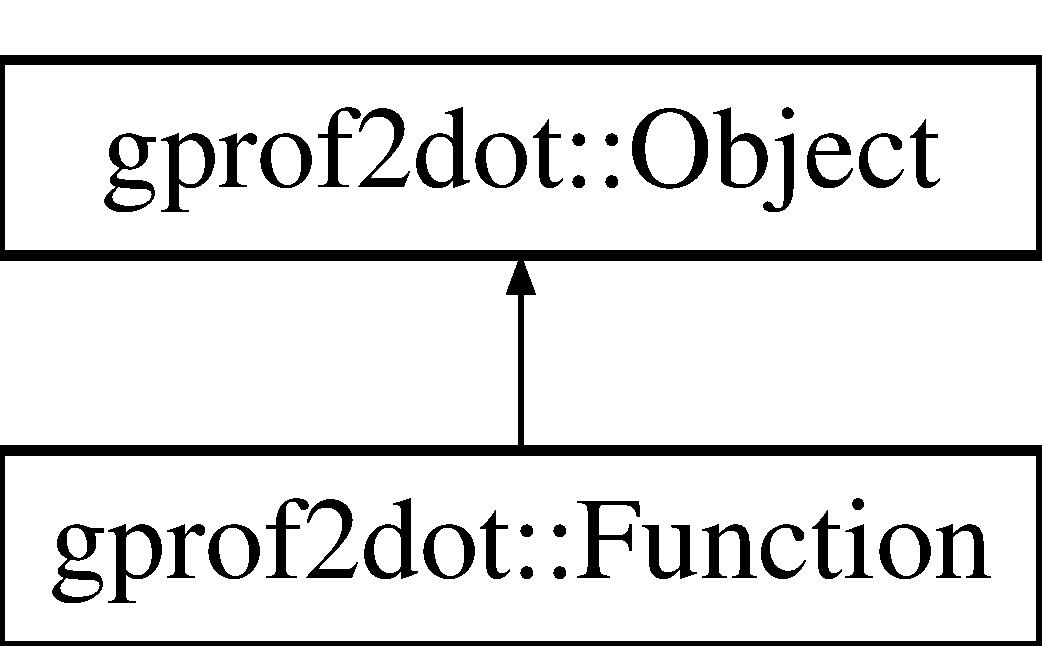
\includegraphics[height=2.000000cm]{classgprof2dot_1_1Function}
\end{center}
\end{figure}
\subsection*{Public Member Functions}
\begin{DoxyCompactItemize}
\item 
def \hyperlink{classgprof2dot_1_1Function_a07309fed1a380e4e2d5715ce4c23f85d}{\_\-\_\-init\_\-\_\-}
\item 
def \hyperlink{classgprof2dot_1_1Function_a7c42628f5fa968e69950cd824daaee53}{add\_\-call}
\item 
def \hyperlink{classgprof2dot_1_1Function_a558d9eb243fd4038571aafefe2b0f2b7}{get\_\-call}
\item 
def \hyperlink{classgprof2dot_1_1Function_a54189eccb9fa937a3740b0a26b01819d}{\_\-\_\-repr\_\-\_\-}
\end{DoxyCompactItemize}
\subsection*{Public Attributes}
\begin{DoxyCompactItemize}
\item 
\hyperlink{classgprof2dot_1_1Function_af94d9542ce8310c4411e8b582799b62c}{id}
\item 
\hyperlink{classgprof2dot_1_1Function_a1a48dee1b5120d74751d874429e539eb}{name}
\item 
\hyperlink{classgprof2dot_1_1Function_aa25a58d197676ff91617109539440b0f}{module}
\item 
\hyperlink{classgprof2dot_1_1Function_a7a0b3e3634324e0db378b9ba1fd896b3}{process}
\item 
\hyperlink{classgprof2dot_1_1Function_aedaa9fad9c10943cd384cf9258e34727}{calls}
\item 
\hyperlink{classgprof2dot_1_1Function_ada8834d7262abe161268d246af697450}{called}
\item 
\hyperlink{classgprof2dot_1_1Function_ab85bab1adeddba144e8d31d75a3179d9}{weight}
\item 
\hyperlink{classgprof2dot_1_1Function_ad15eca167d57acff8004bd22b5c6fd12}{cycle}
\end{DoxyCompactItemize}


\subsection{Detailed Description}
\begin{DoxyVerb}A function.\end{DoxyVerb}
 

\subsection{Constructor \& Destructor Documentation}
\hypertarget{classgprof2dot_1_1Function_a07309fed1a380e4e2d5715ce4c23f85d}{
\index{gprof2dot::Function@{gprof2dot::Function}!\_\-\_\-init\_\-\_\-@{\_\-\_\-init\_\-\_\-}}
\index{\_\-\_\-init\_\-\_\-@{\_\-\_\-init\_\-\_\-}!gprof2dot::Function@{gprof2dot::Function}}
\subsubsection[{\_\-\_\-init\_\-\_\-}]{\setlength{\rightskip}{0pt plus 5cm}def gprof2dot::Function::\_\-\_\-init\_\-\_\- (
\begin{DoxyParamCaption}
\item[{}]{self, }
\item[{}]{id, }
\item[{}]{name}
\end{DoxyParamCaption}
)}}
\label{classgprof2dot_1_1Function_a07309fed1a380e4e2d5715ce4c23f85d}


\subsection{Member Function Documentation}
\hypertarget{classgprof2dot_1_1Function_a54189eccb9fa937a3740b0a26b01819d}{
\index{gprof2dot::Function@{gprof2dot::Function}!\_\-\_\-repr\_\-\_\-@{\_\-\_\-repr\_\-\_\-}}
\index{\_\-\_\-repr\_\-\_\-@{\_\-\_\-repr\_\-\_\-}!gprof2dot::Function@{gprof2dot::Function}}
\subsubsection[{\_\-\_\-repr\_\-\_\-}]{\setlength{\rightskip}{0pt plus 5cm}def gprof2dot::Function::\_\-\_\-repr\_\-\_\- (
\begin{DoxyParamCaption}
\item[{}]{self}
\end{DoxyParamCaption}
)}}
\label{classgprof2dot_1_1Function_a54189eccb9fa937a3740b0a26b01819d}
\hypertarget{classgprof2dot_1_1Function_a7c42628f5fa968e69950cd824daaee53}{
\index{gprof2dot::Function@{gprof2dot::Function}!add\_\-call@{add\_\-call}}
\index{add\_\-call@{add\_\-call}!gprof2dot::Function@{gprof2dot::Function}}
\subsubsection[{add\_\-call}]{\setlength{\rightskip}{0pt plus 5cm}def gprof2dot::Function::add\_\-call (
\begin{DoxyParamCaption}
\item[{}]{self, }
\item[{}]{call}
\end{DoxyParamCaption}
)}}
\label{classgprof2dot_1_1Function_a7c42628f5fa968e69950cd824daaee53}
\hypertarget{classgprof2dot_1_1Function_a558d9eb243fd4038571aafefe2b0f2b7}{
\index{gprof2dot::Function@{gprof2dot::Function}!get\_\-call@{get\_\-call}}
\index{get\_\-call@{get\_\-call}!gprof2dot::Function@{gprof2dot::Function}}
\subsubsection[{get\_\-call}]{\setlength{\rightskip}{0pt plus 5cm}def gprof2dot::Function::get\_\-call (
\begin{DoxyParamCaption}
\item[{}]{self, }
\item[{}]{callee\_\-id}
\end{DoxyParamCaption}
)}}
\label{classgprof2dot_1_1Function_a558d9eb243fd4038571aafefe2b0f2b7}


\subsection{Member Data Documentation}
\hypertarget{classgprof2dot_1_1Function_ada8834d7262abe161268d246af697450}{
\index{gprof2dot::Function@{gprof2dot::Function}!called@{called}}
\index{called@{called}!gprof2dot::Function@{gprof2dot::Function}}
\subsubsection[{called}]{\setlength{\rightskip}{0pt plus 5cm}{\bf gprof2dot::Function::called}}}
\label{classgprof2dot_1_1Function_ada8834d7262abe161268d246af697450}
\hypertarget{classgprof2dot_1_1Function_aedaa9fad9c10943cd384cf9258e34727}{
\index{gprof2dot::Function@{gprof2dot::Function}!calls@{calls}}
\index{calls@{calls}!gprof2dot::Function@{gprof2dot::Function}}
\subsubsection[{calls}]{\setlength{\rightskip}{0pt plus 5cm}{\bf gprof2dot::Function::calls}}}
\label{classgprof2dot_1_1Function_aedaa9fad9c10943cd384cf9258e34727}
\hypertarget{classgprof2dot_1_1Function_ad15eca167d57acff8004bd22b5c6fd12}{
\index{gprof2dot::Function@{gprof2dot::Function}!cycle@{cycle}}
\index{cycle@{cycle}!gprof2dot::Function@{gprof2dot::Function}}
\subsubsection[{cycle}]{\setlength{\rightskip}{0pt plus 5cm}{\bf gprof2dot::Function::cycle}}}
\label{classgprof2dot_1_1Function_ad15eca167d57acff8004bd22b5c6fd12}
\hypertarget{classgprof2dot_1_1Function_af94d9542ce8310c4411e8b582799b62c}{
\index{gprof2dot::Function@{gprof2dot::Function}!id@{id}}
\index{id@{id}!gprof2dot::Function@{gprof2dot::Function}}
\subsubsection[{id}]{\setlength{\rightskip}{0pt plus 5cm}{\bf gprof2dot::Function::id}}}
\label{classgprof2dot_1_1Function_af94d9542ce8310c4411e8b582799b62c}
\hypertarget{classgprof2dot_1_1Function_aa25a58d197676ff91617109539440b0f}{
\index{gprof2dot::Function@{gprof2dot::Function}!module@{module}}
\index{module@{module}!gprof2dot::Function@{gprof2dot::Function}}
\subsubsection[{module}]{\setlength{\rightskip}{0pt plus 5cm}{\bf gprof2dot::Function::module}}}
\label{classgprof2dot_1_1Function_aa25a58d197676ff91617109539440b0f}
\hypertarget{classgprof2dot_1_1Function_a1a48dee1b5120d74751d874429e539eb}{
\index{gprof2dot::Function@{gprof2dot::Function}!name@{name}}
\index{name@{name}!gprof2dot::Function@{gprof2dot::Function}}
\subsubsection[{name}]{\setlength{\rightskip}{0pt plus 5cm}{\bf gprof2dot::Function::name}}}
\label{classgprof2dot_1_1Function_a1a48dee1b5120d74751d874429e539eb}
\hypertarget{classgprof2dot_1_1Function_a7a0b3e3634324e0db378b9ba1fd896b3}{
\index{gprof2dot::Function@{gprof2dot::Function}!process@{process}}
\index{process@{process}!gprof2dot::Function@{gprof2dot::Function}}
\subsubsection[{process}]{\setlength{\rightskip}{0pt plus 5cm}{\bf gprof2dot::Function::process}}}
\label{classgprof2dot_1_1Function_a7a0b3e3634324e0db378b9ba1fd896b3}
\hypertarget{classgprof2dot_1_1Function_ab85bab1adeddba144e8d31d75a3179d9}{
\index{gprof2dot::Function@{gprof2dot::Function}!weight@{weight}}
\index{weight@{weight}!gprof2dot::Function@{gprof2dot::Function}}
\subsubsection[{weight}]{\setlength{\rightskip}{0pt plus 5cm}{\bf gprof2dot::Function::weight}}}
\label{classgprof2dot_1_1Function_ab85bab1adeddba144e8d31d75a3179d9}


The documentation for this class was generated from the following file:\begin{DoxyCompactItemize}
\item 
\hyperlink{gprof2dot_8py}{gprof2dot.py}\end{DoxyCompactItemize}

\hypertarget{classgprof2dot_1_1GprofParser}{
\section{gprof2dot::GprofParser Class Reference}
\label{classgprof2dot_1_1GprofParser}\index{gprof2dot::GprofParser@{gprof2dot::GprofParser}}
}
Inheritance diagram for gprof2dot::GprofParser:\begin{figure}[H]
\begin{center}
\leavevmode
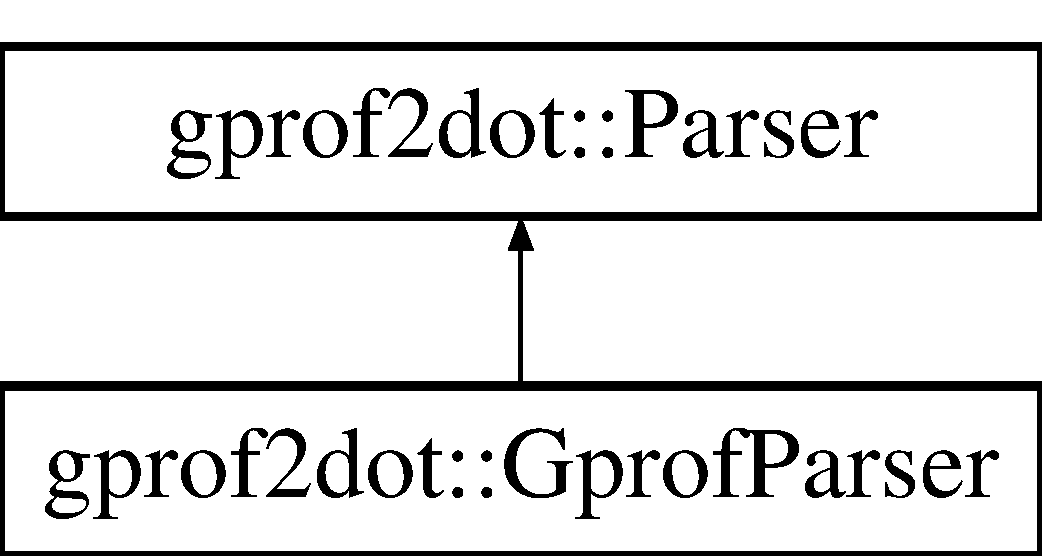
\includegraphics[height=2.000000cm]{classgprof2dot_1_1GprofParser}
\end{center}
\end{figure}
\subsection*{Public Member Functions}
\begin{DoxyCompactItemize}
\item 
def \hyperlink{classgprof2dot_1_1GprofParser_acacfb5c014ebdc5b5f0ea25cad4fec6f}{\_\-\_\-init\_\-\_\-}
\item 
def \hyperlink{classgprof2dot_1_1GprofParser_a5ab276c4c9abcc71d917ea14f73511eb}{readline}
\item 
def \hyperlink{classgprof2dot_1_1GprofParser_a2f7fb2ffdfdf923f74f22177baaccc40}{translate}
\item 
def \hyperlink{classgprof2dot_1_1GprofParser_abd32e64d5745ce238a90343bbf7f6bad}{parse\_\-function\_\-entry}
\item 
def \hyperlink{classgprof2dot_1_1GprofParser_a175b0a9f7484eb6f1da3e94a31eaf0ac}{parse\_\-cycle\_\-entry}
\item 
def \hyperlink{classgprof2dot_1_1GprofParser_a95fad2a05c6ca70256d7a25c56aa29cb}{parse\_\-cg\_\-entry}
\item 
def \hyperlink{classgprof2dot_1_1GprofParser_a71d6b6f813e70ca931dacdfc64d0b183}{parse\_\-cg}
\item 
def \hyperlink{classgprof2dot_1_1GprofParser_a840c96752592fffdb69514cf59022705}{parse}
\end{DoxyCompactItemize}
\subsection*{Public Attributes}
\begin{DoxyCompactItemize}
\item 
\hyperlink{classgprof2dot_1_1GprofParser_a65b9a8783fe4aea6e72e67f041c126b2}{fp}
\item 
\hyperlink{classgprof2dot_1_1GprofParser_a7459094ba27540637888860ccea69720}{functions}
\item 
\hyperlink{classgprof2dot_1_1GprofParser_a5a17f96d4420c651af6b955c221c43c9}{cycles}
\end{DoxyCompactItemize}


\subsection{Detailed Description}
\begin{DoxyVerb}Parser for GNU gprof output.

See also:
- Chapter "Interpreting gprof's Output" from the GNU gprof manual
  http://sourceware.org/binutils/docs-2.18/gprof/Call-Graph.html#Call-Graph
- File "cg_print.c" from the GNU gprof source code
  http://sourceware.org/cgi-bin/cvsweb.cgi/~checkout~/src/gprof/cg_print.c?rev=1.12&cvsroot=src
\end{DoxyVerb}
 

\subsection{Constructor \& Destructor Documentation}
\hypertarget{classgprof2dot_1_1GprofParser_acacfb5c014ebdc5b5f0ea25cad4fec6f}{
\index{gprof2dot::GprofParser@{gprof2dot::GprofParser}!\_\-\_\-init\_\-\_\-@{\_\-\_\-init\_\-\_\-}}
\index{\_\-\_\-init\_\-\_\-@{\_\-\_\-init\_\-\_\-}!gprof2dot::GprofParser@{gprof2dot::GprofParser}}
\subsubsection[{\_\-\_\-init\_\-\_\-}]{\setlength{\rightskip}{0pt plus 5cm}def gprof2dot::GprofParser::\_\-\_\-init\_\-\_\- (
\begin{DoxyParamCaption}
\item[{}]{self, }
\item[{}]{fp}
\end{DoxyParamCaption}
)}}
\label{classgprof2dot_1_1GprofParser_acacfb5c014ebdc5b5f0ea25cad4fec6f}


\subsection{Member Function Documentation}
\hypertarget{classgprof2dot_1_1GprofParser_a840c96752592fffdb69514cf59022705}{
\index{gprof2dot::GprofParser@{gprof2dot::GprofParser}!parse@{parse}}
\index{parse@{parse}!gprof2dot::GprofParser@{gprof2dot::GprofParser}}
\subsubsection[{parse}]{\setlength{\rightskip}{0pt plus 5cm}def gprof2dot::GprofParser::parse (
\begin{DoxyParamCaption}
\item[{}]{self}
\end{DoxyParamCaption}
)}}
\label{classgprof2dot_1_1GprofParser_a840c96752592fffdb69514cf59022705}


Reimplemented from \hyperlink{classgprof2dot_1_1Parser_a681a0bc74e640c9c8e3d629dd03049fc}{gprof2dot::Parser}.

\hypertarget{classgprof2dot_1_1GprofParser_a71d6b6f813e70ca931dacdfc64d0b183}{
\index{gprof2dot::GprofParser@{gprof2dot::GprofParser}!parse\_\-cg@{parse\_\-cg}}
\index{parse\_\-cg@{parse\_\-cg}!gprof2dot::GprofParser@{gprof2dot::GprofParser}}
\subsubsection[{parse\_\-cg}]{\setlength{\rightskip}{0pt plus 5cm}def gprof2dot::GprofParser::parse\_\-cg (
\begin{DoxyParamCaption}
\item[{}]{self}
\end{DoxyParamCaption}
)}}
\label{classgprof2dot_1_1GprofParser_a71d6b6f813e70ca931dacdfc64d0b183}
\begin{DoxyVerb}Parse the call graph.\end{DoxyVerb}
 \hypertarget{classgprof2dot_1_1GprofParser_a95fad2a05c6ca70256d7a25c56aa29cb}{
\index{gprof2dot::GprofParser@{gprof2dot::GprofParser}!parse\_\-cg\_\-entry@{parse\_\-cg\_\-entry}}
\index{parse\_\-cg\_\-entry@{parse\_\-cg\_\-entry}!gprof2dot::GprofParser@{gprof2dot::GprofParser}}
\subsubsection[{parse\_\-cg\_\-entry}]{\setlength{\rightskip}{0pt plus 5cm}def gprof2dot::GprofParser::parse\_\-cg\_\-entry (
\begin{DoxyParamCaption}
\item[{}]{self, }
\item[{}]{lines}
\end{DoxyParamCaption}
)}}
\label{classgprof2dot_1_1GprofParser_a95fad2a05c6ca70256d7a25c56aa29cb}
\hypertarget{classgprof2dot_1_1GprofParser_a175b0a9f7484eb6f1da3e94a31eaf0ac}{
\index{gprof2dot::GprofParser@{gprof2dot::GprofParser}!parse\_\-cycle\_\-entry@{parse\_\-cycle\_\-entry}}
\index{parse\_\-cycle\_\-entry@{parse\_\-cycle\_\-entry}!gprof2dot::GprofParser@{gprof2dot::GprofParser}}
\subsubsection[{parse\_\-cycle\_\-entry}]{\setlength{\rightskip}{0pt plus 5cm}def gprof2dot::GprofParser::parse\_\-cycle\_\-entry (
\begin{DoxyParamCaption}
\item[{}]{self, }
\item[{}]{lines}
\end{DoxyParamCaption}
)}}
\label{classgprof2dot_1_1GprofParser_a175b0a9f7484eb6f1da3e94a31eaf0ac}
\hypertarget{classgprof2dot_1_1GprofParser_abd32e64d5745ce238a90343bbf7f6bad}{
\index{gprof2dot::GprofParser@{gprof2dot::GprofParser}!parse\_\-function\_\-entry@{parse\_\-function\_\-entry}}
\index{parse\_\-function\_\-entry@{parse\_\-function\_\-entry}!gprof2dot::GprofParser@{gprof2dot::GprofParser}}
\subsubsection[{parse\_\-function\_\-entry}]{\setlength{\rightskip}{0pt plus 5cm}def gprof2dot::GprofParser::parse\_\-function\_\-entry (
\begin{DoxyParamCaption}
\item[{}]{self, }
\item[{}]{lines}
\end{DoxyParamCaption}
)}}
\label{classgprof2dot_1_1GprofParser_abd32e64d5745ce238a90343bbf7f6bad}
\hypertarget{classgprof2dot_1_1GprofParser_a5ab276c4c9abcc71d917ea14f73511eb}{
\index{gprof2dot::GprofParser@{gprof2dot::GprofParser}!readline@{readline}}
\index{readline@{readline}!gprof2dot::GprofParser@{gprof2dot::GprofParser}}
\subsubsection[{readline}]{\setlength{\rightskip}{0pt plus 5cm}def gprof2dot::GprofParser::readline (
\begin{DoxyParamCaption}
\item[{}]{self}
\end{DoxyParamCaption}
)}}
\label{classgprof2dot_1_1GprofParser_a5ab276c4c9abcc71d917ea14f73511eb}
\hypertarget{classgprof2dot_1_1GprofParser_a2f7fb2ffdfdf923f74f22177baaccc40}{
\index{gprof2dot::GprofParser@{gprof2dot::GprofParser}!translate@{translate}}
\index{translate@{translate}!gprof2dot::GprofParser@{gprof2dot::GprofParser}}
\subsubsection[{translate}]{\setlength{\rightskip}{0pt plus 5cm}def gprof2dot::GprofParser::translate (
\begin{DoxyParamCaption}
\item[{}]{self, }
\item[{}]{mo}
\end{DoxyParamCaption}
)}}
\label{classgprof2dot_1_1GprofParser_a2f7fb2ffdfdf923f74f22177baaccc40}
\begin{DoxyVerb}Extract a structure from a match object, while translating the types in the process.\end{DoxyVerb}
 

\subsection{Member Data Documentation}
\hypertarget{classgprof2dot_1_1GprofParser_a5a17f96d4420c651af6b955c221c43c9}{
\index{gprof2dot::GprofParser@{gprof2dot::GprofParser}!cycles@{cycles}}
\index{cycles@{cycles}!gprof2dot::GprofParser@{gprof2dot::GprofParser}}
\subsubsection[{cycles}]{\setlength{\rightskip}{0pt plus 5cm}{\bf gprof2dot::GprofParser::cycles}}}
\label{classgprof2dot_1_1GprofParser_a5a17f96d4420c651af6b955c221c43c9}
\hypertarget{classgprof2dot_1_1GprofParser_a65b9a8783fe4aea6e72e67f041c126b2}{
\index{gprof2dot::GprofParser@{gprof2dot::GprofParser}!fp@{fp}}
\index{fp@{fp}!gprof2dot::GprofParser@{gprof2dot::GprofParser}}
\subsubsection[{fp}]{\setlength{\rightskip}{0pt plus 5cm}{\bf gprof2dot::GprofParser::fp}}}
\label{classgprof2dot_1_1GprofParser_a65b9a8783fe4aea6e72e67f041c126b2}
\hypertarget{classgprof2dot_1_1GprofParser_a7459094ba27540637888860ccea69720}{
\index{gprof2dot::GprofParser@{gprof2dot::GprofParser}!functions@{functions}}
\index{functions@{functions}!gprof2dot::GprofParser@{gprof2dot::GprofParser}}
\subsubsection[{functions}]{\setlength{\rightskip}{0pt plus 5cm}{\bf gprof2dot::GprofParser::functions}}}
\label{classgprof2dot_1_1GprofParser_a7459094ba27540637888860ccea69720}


The documentation for this class was generated from the following file:\begin{DoxyCompactItemize}
\item 
\hyperlink{gprof2dot_8py}{gprof2dot.py}\end{DoxyCompactItemize}

\hypertarget{classgprof2dot_1_1HProfParser}{
\section{gprof2dot::HProfParser Class Reference}
\label{classgprof2dot_1_1HProfParser}\index{gprof2dot::HProfParser@{gprof2dot::HProfParser}}
}
Inheritance diagram for gprof2dot::HProfParser:\begin{figure}[H]
\begin{center}
\leavevmode
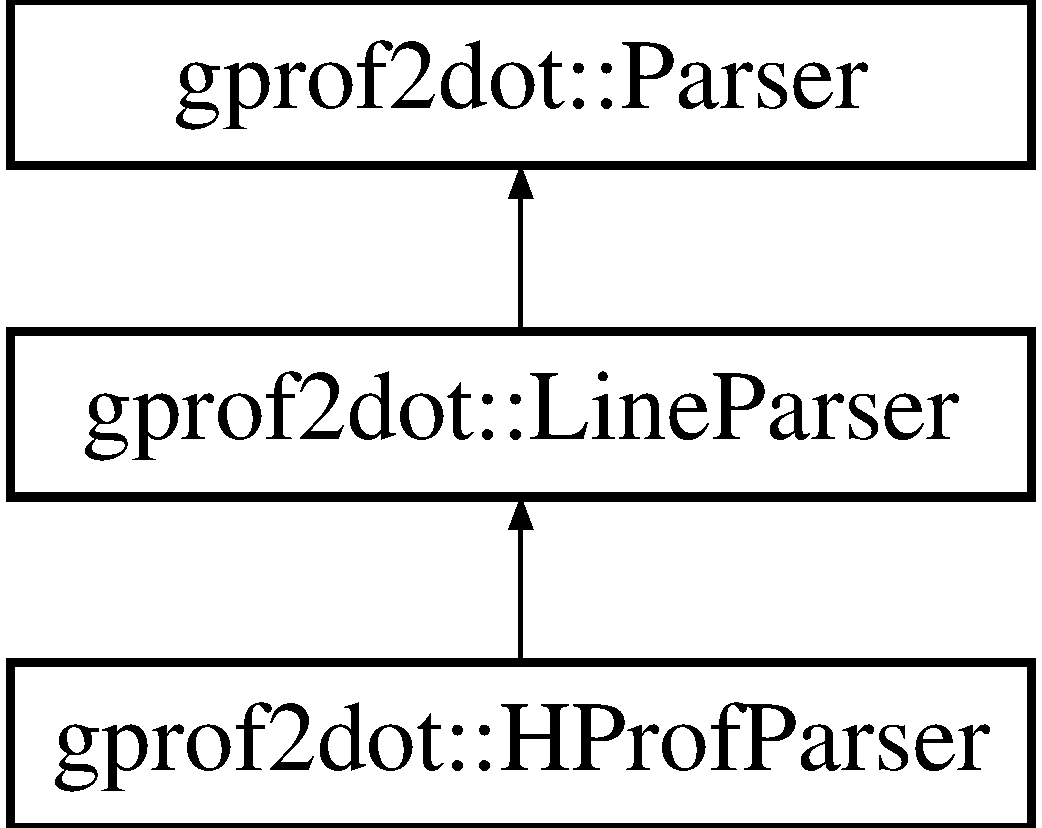
\includegraphics[height=3.000000cm]{classgprof2dot_1_1HProfParser}
\end{center}
\end{figure}
\subsection*{Public Member Functions}
\begin{DoxyCompactItemize}
\item 
def \hyperlink{classgprof2dot_1_1HProfParser_a1bc12e0ba546db9789dd34a30ea650ea}{\_\-\_\-init\_\-\_\-}
\item 
def \hyperlink{classgprof2dot_1_1HProfParser_a8f6dc9e1899c27794ccc8676a33d62fa}{parse}
\item 
def \hyperlink{classgprof2dot_1_1HProfParser_ae7545eac0c68cd11916091f500fe41ef}{parse\_\-traces}
\item 
def \hyperlink{classgprof2dot_1_1HProfParser_a82bdb213a803b654111054f7fe2645f2}{parse\_\-trace}
\item 
def \hyperlink{classgprof2dot_1_1HProfParser_a9a8a3aa2a0c23e441b1943f19ef7b10c}{parse\_\-samples}
\end{DoxyCompactItemize}
\subsection*{Public Attributes}
\begin{DoxyCompactItemize}
\item 
\hyperlink{classgprof2dot_1_1HProfParser_af9da484ae6aff23799453b827b926289}{traces}
\item 
\hyperlink{classgprof2dot_1_1HProfParser_a3c0310fc0ef8b98ae09fa94f36f116d5}{samples}
\end{DoxyCompactItemize}
\subsection*{Static Public Attributes}
\begin{DoxyCompactItemize}
\item 
tuple \hyperlink{classgprof2dot_1_1HProfParser_af71eae81a0a57ed7b7210364ee666679}{trace\_\-re} = re.compile(r'$\backslash$t(.$\ast$)$\backslash$((.$\ast$):(.$\ast$)$\backslash$)')
\item 
tuple \hyperlink{classgprof2dot_1_1HProfParser_a299919246c94ae17e7293fd9908ab071}{trace\_\-id\_\-re} = re.compile(r'$^\wedge$TRACE ($\backslash$d+):\$')
\end{DoxyCompactItemize}


\subsection{Detailed Description}
\begin{DoxyVerb}Parser for java hprof output

See also:
- http://java.sun.com/developer/technicalArticles/Programming/HPROF.html
\end{DoxyVerb}
 

\subsection{Constructor \& Destructor Documentation}
\hypertarget{classgprof2dot_1_1HProfParser_a1bc12e0ba546db9789dd34a30ea650ea}{
\index{gprof2dot::HProfParser@{gprof2dot::HProfParser}!\_\-\_\-init\_\-\_\-@{\_\-\_\-init\_\-\_\-}}
\index{\_\-\_\-init\_\-\_\-@{\_\-\_\-init\_\-\_\-}!gprof2dot::HProfParser@{gprof2dot::HProfParser}}
\subsubsection[{\_\-\_\-init\_\-\_\-}]{\setlength{\rightskip}{0pt plus 5cm}def gprof2dot::HProfParser::\_\-\_\-init\_\-\_\- (
\begin{DoxyParamCaption}
\item[{}]{self, }
\item[{}]{infile}
\end{DoxyParamCaption}
)}}
\label{classgprof2dot_1_1HProfParser_a1bc12e0ba546db9789dd34a30ea650ea}


Reimplemented from \hyperlink{classgprof2dot_1_1LineParser_a9ab24f364f64a70181dd4156cea194c5}{gprof2dot::LineParser}.



\subsection{Member Function Documentation}
\hypertarget{classgprof2dot_1_1HProfParser_a8f6dc9e1899c27794ccc8676a33d62fa}{
\index{gprof2dot::HProfParser@{gprof2dot::HProfParser}!parse@{parse}}
\index{parse@{parse}!gprof2dot::HProfParser@{gprof2dot::HProfParser}}
\subsubsection[{parse}]{\setlength{\rightskip}{0pt plus 5cm}def gprof2dot::HProfParser::parse (
\begin{DoxyParamCaption}
\item[{}]{self}
\end{DoxyParamCaption}
)}}
\label{classgprof2dot_1_1HProfParser_a8f6dc9e1899c27794ccc8676a33d62fa}


Reimplemented from \hyperlink{classgprof2dot_1_1Parser_a681a0bc74e640c9c8e3d629dd03049fc}{gprof2dot::Parser}.

\hypertarget{classgprof2dot_1_1HProfParser_a9a8a3aa2a0c23e441b1943f19ef7b10c}{
\index{gprof2dot::HProfParser@{gprof2dot::HProfParser}!parse\_\-samples@{parse\_\-samples}}
\index{parse\_\-samples@{parse\_\-samples}!gprof2dot::HProfParser@{gprof2dot::HProfParser}}
\subsubsection[{parse\_\-samples}]{\setlength{\rightskip}{0pt plus 5cm}def gprof2dot::HProfParser::parse\_\-samples (
\begin{DoxyParamCaption}
\item[{}]{self}
\end{DoxyParamCaption}
)}}
\label{classgprof2dot_1_1HProfParser_a9a8a3aa2a0c23e441b1943f19ef7b10c}
\hypertarget{classgprof2dot_1_1HProfParser_a82bdb213a803b654111054f7fe2645f2}{
\index{gprof2dot::HProfParser@{gprof2dot::HProfParser}!parse\_\-trace@{parse\_\-trace}}
\index{parse\_\-trace@{parse\_\-trace}!gprof2dot::HProfParser@{gprof2dot::HProfParser}}
\subsubsection[{parse\_\-trace}]{\setlength{\rightskip}{0pt plus 5cm}def gprof2dot::HProfParser::parse\_\-trace (
\begin{DoxyParamCaption}
\item[{}]{self}
\end{DoxyParamCaption}
)}}
\label{classgprof2dot_1_1HProfParser_a82bdb213a803b654111054f7fe2645f2}
\hypertarget{classgprof2dot_1_1HProfParser_ae7545eac0c68cd11916091f500fe41ef}{
\index{gprof2dot::HProfParser@{gprof2dot::HProfParser}!parse\_\-traces@{parse\_\-traces}}
\index{parse\_\-traces@{parse\_\-traces}!gprof2dot::HProfParser@{gprof2dot::HProfParser}}
\subsubsection[{parse\_\-traces}]{\setlength{\rightskip}{0pt plus 5cm}def gprof2dot::HProfParser::parse\_\-traces (
\begin{DoxyParamCaption}
\item[{}]{self}
\end{DoxyParamCaption}
)}}
\label{classgprof2dot_1_1HProfParser_ae7545eac0c68cd11916091f500fe41ef}


\subsection{Member Data Documentation}
\hypertarget{classgprof2dot_1_1HProfParser_a3c0310fc0ef8b98ae09fa94f36f116d5}{
\index{gprof2dot::HProfParser@{gprof2dot::HProfParser}!samples@{samples}}
\index{samples@{samples}!gprof2dot::HProfParser@{gprof2dot::HProfParser}}
\subsubsection[{samples}]{\setlength{\rightskip}{0pt plus 5cm}{\bf gprof2dot::HProfParser::samples}}}
\label{classgprof2dot_1_1HProfParser_a3c0310fc0ef8b98ae09fa94f36f116d5}
\hypertarget{classgprof2dot_1_1HProfParser_a299919246c94ae17e7293fd9908ab071}{
\index{gprof2dot::HProfParser@{gprof2dot::HProfParser}!trace\_\-id\_\-re@{trace\_\-id\_\-re}}
\index{trace\_\-id\_\-re@{trace\_\-id\_\-re}!gprof2dot::HProfParser@{gprof2dot::HProfParser}}
\subsubsection[{trace\_\-id\_\-re}]{\setlength{\rightskip}{0pt plus 5cm}tuple {\bf gprof2dot::HProfParser::trace\_\-id\_\-re} = re.compile(r'$^\wedge$TRACE ($\backslash$d+):\$')\hspace{0.3cm}{\ttfamily  \mbox{[}static\mbox{]}}}}
\label{classgprof2dot_1_1HProfParser_a299919246c94ae17e7293fd9908ab071}
\hypertarget{classgprof2dot_1_1HProfParser_af71eae81a0a57ed7b7210364ee666679}{
\index{gprof2dot::HProfParser@{gprof2dot::HProfParser}!trace\_\-re@{trace\_\-re}}
\index{trace\_\-re@{trace\_\-re}!gprof2dot::HProfParser@{gprof2dot::HProfParser}}
\subsubsection[{trace\_\-re}]{\setlength{\rightskip}{0pt plus 5cm}tuple {\bf gprof2dot::HProfParser::trace\_\-re} = re.compile(r'$\backslash$t(.$\ast$)$\backslash$((.$\ast$):(.$\ast$)$\backslash$)')\hspace{0.3cm}{\ttfamily  \mbox{[}static\mbox{]}}}}
\label{classgprof2dot_1_1HProfParser_af71eae81a0a57ed7b7210364ee666679}
\hypertarget{classgprof2dot_1_1HProfParser_af9da484ae6aff23799453b827b926289}{
\index{gprof2dot::HProfParser@{gprof2dot::HProfParser}!traces@{traces}}
\index{traces@{traces}!gprof2dot::HProfParser@{gprof2dot::HProfParser}}
\subsubsection[{traces}]{\setlength{\rightskip}{0pt plus 5cm}{\bf gprof2dot::HProfParser::traces}}}
\label{classgprof2dot_1_1HProfParser_af9da484ae6aff23799453b827b926289}


The documentation for this class was generated from the following file:\begin{DoxyCompactItemize}
\item 
\hyperlink{gprof2dot_8py}{gprof2dot.py}\end{DoxyCompactItemize}

\hypertarget{structExecutor_1_1Job}{
\section{Executor::Job Struct Reference}
\label{structExecutor_1_1Job}\index{Executor::Job@{Executor::Job}}
}


Estrutura que representa um job. Guarda os dados necessarios para controlar processos.  




{\ttfamily \#include $<$Executor.hpp$>$}

\subsection*{Public Member Functions}
\begin{DoxyCompactItemize}
\item 
\hyperlink{structExecutor_1_1Job_aa6e1a092856e7ebc043adfb1eaa2c627}{Job} ()
\end{DoxyCompactItemize}
\subsection*{Public Attributes}
\begin{DoxyCompactItemize}
\item 
std::string \hyperlink{structExecutor_1_1Job_a38039efac2d62af668c99b63719f6125}{name}
\item 
pid\_\-t \hyperlink{structExecutor_1_1Job_a8d9163526e877fe1f603b66504ef8950}{pid}
\item 
unsigned \hyperlink{structExecutor_1_1Job_a9429fceffd304e1666ba1e8d0495c3f9}{jobid}
\item 
unsigned \hyperlink{structExecutor_1_1Job_ab3f85f9152e9b5457896f1b72fa8508c}{groupid}
\item 
bool \hyperlink{structExecutor_1_1Job_ac0ea0bc0c71fe4c1a2ad981df09fb5b0}{stopped}
\item 
bool \hyperlink{structExecutor_1_1Job_a7574b1ef35cd0dace06aee928fead108}{dead}
\end{DoxyCompactItemize}


\subsection{Detailed Description}
Estrutura que representa um job. Guarda os dados necessarios para controlar processos. \begin{DoxySeeAlso}{See also}
\hyperlink{classExecutor}{Executor} 
\end{DoxySeeAlso}


\subsection{Constructor \& Destructor Documentation}
\hypertarget{structExecutor_1_1Job_aa6e1a092856e7ebc043adfb1eaa2c627}{
\index{Executor::Job@{Executor::Job}!Job@{Job}}
\index{Job@{Job}!Executor::Job@{Executor::Job}}
\subsubsection[{Job}]{\setlength{\rightskip}{0pt plus 5cm}Executor::Job::Job (
\begin{DoxyParamCaption}
{}
\end{DoxyParamCaption}
)}}
\label{structExecutor_1_1Job_aa6e1a092856e7ebc043adfb1eaa2c627}


\subsection{Member Data Documentation}
\hypertarget{structExecutor_1_1Job_a7574b1ef35cd0dace06aee928fead108}{
\index{Executor::Job@{Executor::Job}!dead@{dead}}
\index{dead@{dead}!Executor::Job@{Executor::Job}}
\subsubsection[{dead}]{\setlength{\rightskip}{0pt plus 5cm}bool {\bf Executor::Job::dead}}}
\label{structExecutor_1_1Job_a7574b1ef35cd0dace06aee928fead108}
\hypertarget{structExecutor_1_1Job_ab3f85f9152e9b5457896f1b72fa8508c}{
\index{Executor::Job@{Executor::Job}!groupid@{groupid}}
\index{groupid@{groupid}!Executor::Job@{Executor::Job}}
\subsubsection[{groupid}]{\setlength{\rightskip}{0pt plus 5cm}unsigned {\bf Executor::Job::groupid}}}
\label{structExecutor_1_1Job_ab3f85f9152e9b5457896f1b72fa8508c}
\hypertarget{structExecutor_1_1Job_a9429fceffd304e1666ba1e8d0495c3f9}{
\index{Executor::Job@{Executor::Job}!jobid@{jobid}}
\index{jobid@{jobid}!Executor::Job@{Executor::Job}}
\subsubsection[{jobid}]{\setlength{\rightskip}{0pt plus 5cm}unsigned {\bf Executor::Job::jobid}}}
\label{structExecutor_1_1Job_a9429fceffd304e1666ba1e8d0495c3f9}
\hypertarget{structExecutor_1_1Job_a38039efac2d62af668c99b63719f6125}{
\index{Executor::Job@{Executor::Job}!name@{name}}
\index{name@{name}!Executor::Job@{Executor::Job}}
\subsubsection[{name}]{\setlength{\rightskip}{0pt plus 5cm}std::string {\bf Executor::Job::name}}}
\label{structExecutor_1_1Job_a38039efac2d62af668c99b63719f6125}
\hypertarget{structExecutor_1_1Job_a8d9163526e877fe1f603b66504ef8950}{
\index{Executor::Job@{Executor::Job}!pid@{pid}}
\index{pid@{pid}!Executor::Job@{Executor::Job}}
\subsubsection[{pid}]{\setlength{\rightskip}{0pt plus 5cm}pid\_\-t {\bf Executor::Job::pid}}}
\label{structExecutor_1_1Job_a8d9163526e877fe1f603b66504ef8950}
\hypertarget{structExecutor_1_1Job_ac0ea0bc0c71fe4c1a2ad981df09fb5b0}{
\index{Executor::Job@{Executor::Job}!stopped@{stopped}}
\index{stopped@{stopped}!Executor::Job@{Executor::Job}}
\subsubsection[{stopped}]{\setlength{\rightskip}{0pt plus 5cm}bool {\bf Executor::Job::stopped}}}
\label{structExecutor_1_1Job_ac0ea0bc0c71fe4c1a2ad981df09fb5b0}


The documentation for this struct was generated from the following files:\begin{DoxyCompactItemize}
\item 
\hyperlink{Executor_8hpp}{Executor.hpp}\item 
\hyperlink{Executor_8cpp}{Executor.cpp}\end{DoxyCompactItemize}

\hypertarget{classJobsCommand}{
\section{JobsCommand Class Reference}
\label{classJobsCommand}\index{JobsCommand@{JobsCommand}}
}


Classe que implementa o comando jobs.  




{\ttfamily \#include $<$Builtin.hpp$>$}

Inheritance diagram for JobsCommand:\begin{figure}[H]
\begin{center}
\leavevmode
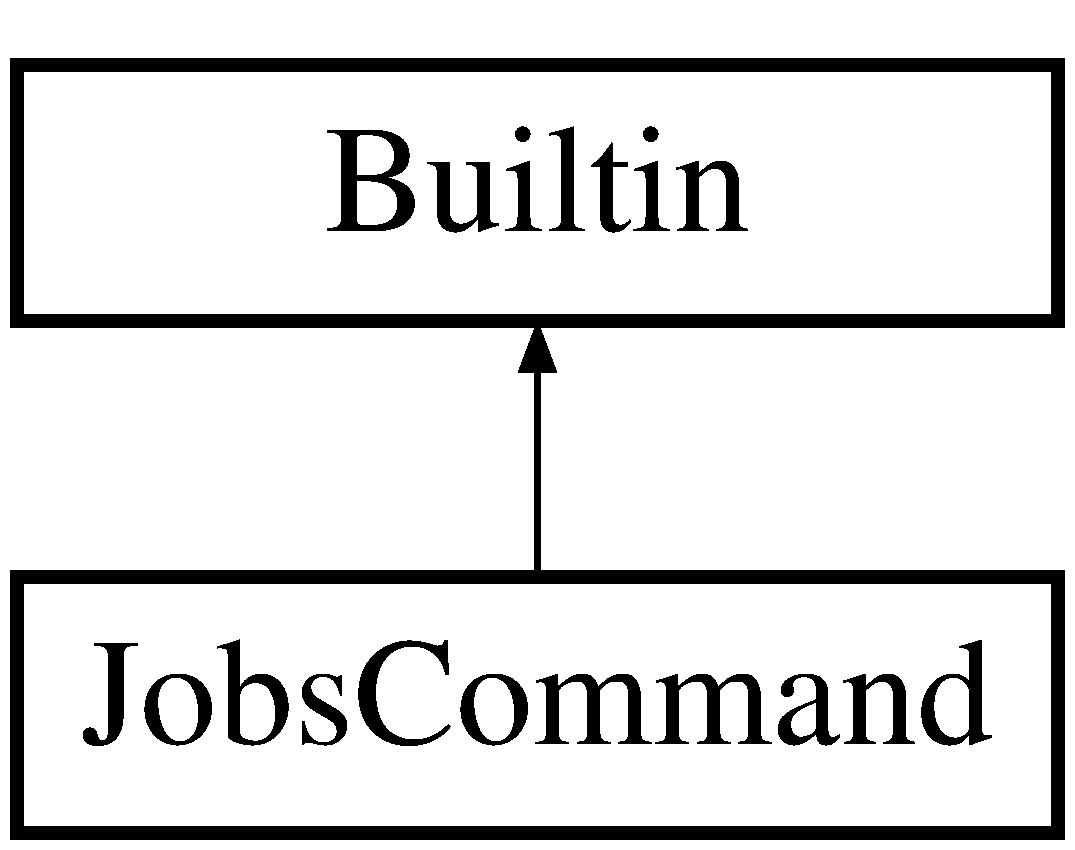
\includegraphics[height=2.000000cm]{classJobsCommand}
\end{center}
\end{figure}


\subsection{Detailed Description}
Classe que implementa o comando jobs. Sintaxe: jobs 

The documentation for this class was generated from the following files:\begin{DoxyCompactItemize}
\item 
\hyperlink{Builtin_8hpp}{Builtin.hpp}\item 
\hyperlink{Builtin_8cpp}{Builtin.cpp}\end{DoxyCompactItemize}

\hypertarget{classKillCommand}{
\section{KillCommand Class Reference}
\label{classKillCommand}\index{KillCommand@{KillCommand}}
}


Classe que implementa o comando kill.  




{\ttfamily \#include $<$Builtin.hpp$>$}

Inheritance diagram for KillCommand:\begin{figure}[H]
\begin{center}
\leavevmode
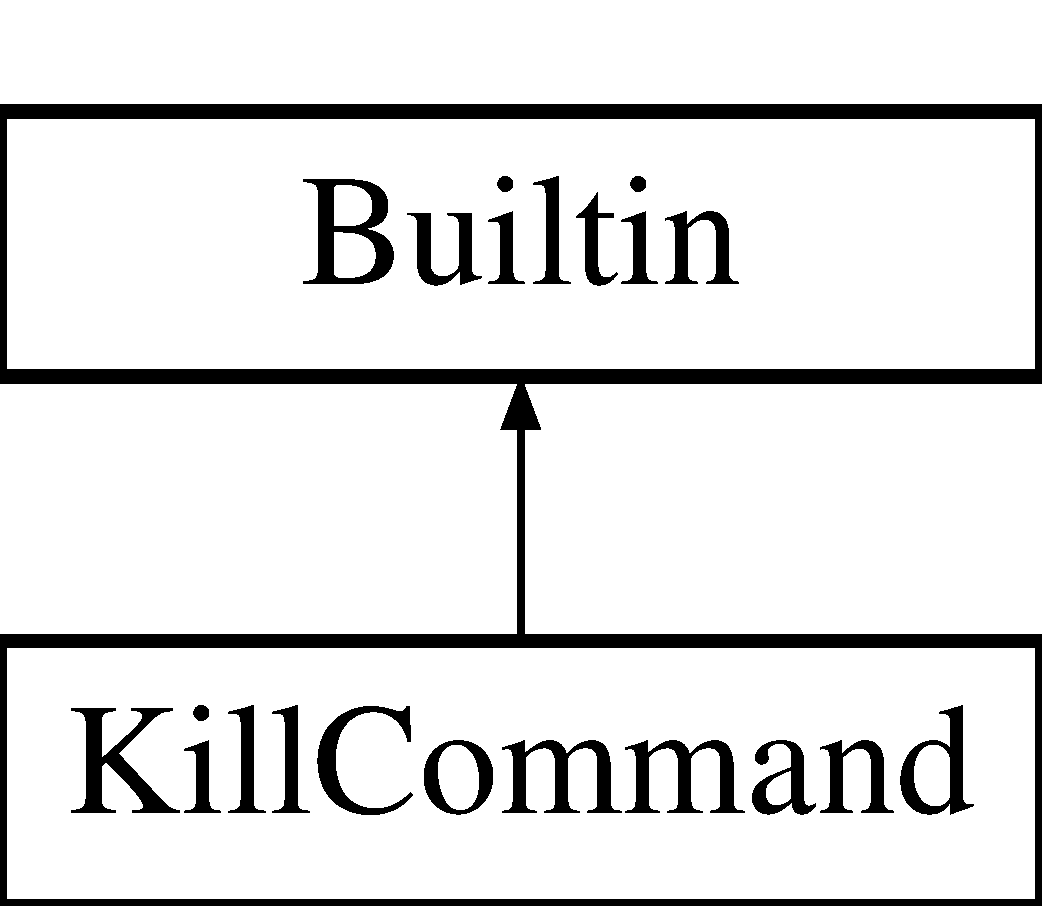
\includegraphics[height=2.000000cm]{classKillCommand}
\end{center}
\end{figure}


\subsection{Detailed Description}
Classe que implementa o comando kill. Sintaxe: kill \%$<$JOBID$>$ 

The documentation for this class was generated from the following files:\begin{DoxyCompactItemize}
\item 
\hyperlink{Builtin_8hpp}{Builtin.hpp}\item 
\hyperlink{Builtin_8cpp}{Builtin.cpp}\end{DoxyCompactItemize}

\hypertarget{classgprof2dot_1_1LineParser}{
\section{gprof2dot::LineParser Class Reference}
\label{classgprof2dot_1_1LineParser}\index{gprof2dot::LineParser@{gprof2dot::LineParser}}
}
Inheritance diagram for gprof2dot::LineParser:\begin{figure}[H]
\begin{center}
\leavevmode
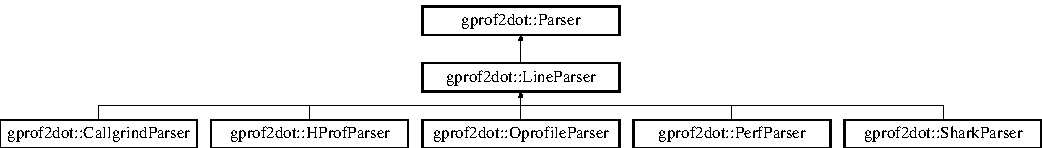
\includegraphics[height=1.988166cm]{classgprof2dot_1_1LineParser}
\end{center}
\end{figure}
\subsection*{Public Member Functions}
\begin{DoxyCompactItemize}
\item 
def \hyperlink{classgprof2dot_1_1LineParser_a9ab24f364f64a70181dd4156cea194c5}{\_\-\_\-init\_\-\_\-}
\item 
def \hyperlink{classgprof2dot_1_1LineParser_aca122098675f8464f11a287ab3660795}{readline}
\item 
def \hyperlink{classgprof2dot_1_1LineParser_ac8ee85c45c20f2a1b041b96b89bdf34c}{lookahead}
\item 
def \hyperlink{classgprof2dot_1_1LineParser_a39083cedf3f4f3ed40a410815f393942}{consume}
\item 
def \hyperlink{classgprof2dot_1_1LineParser_a84fe7464a543da7c585a247f4d603123}{eof}
\end{DoxyCompactItemize}
\subsection*{Public Attributes}
\begin{DoxyCompactItemize}
\item 
\hyperlink{classgprof2dot_1_1LineParser_aab8c55a9d00cb279553751f524e147f2}{line\_\-no}
\end{DoxyCompactItemize}


\subsection{Detailed Description}
\begin{DoxyVerb}Base class for parsers that read line-based formats.\end{DoxyVerb}
 

\subsection{Constructor \& Destructor Documentation}
\hypertarget{classgprof2dot_1_1LineParser_a9ab24f364f64a70181dd4156cea194c5}{
\index{gprof2dot::LineParser@{gprof2dot::LineParser}!\_\-\_\-init\_\-\_\-@{\_\-\_\-init\_\-\_\-}}
\index{\_\-\_\-init\_\-\_\-@{\_\-\_\-init\_\-\_\-}!gprof2dot::LineParser@{gprof2dot::LineParser}}
\subsubsection[{\_\-\_\-init\_\-\_\-}]{\setlength{\rightskip}{0pt plus 5cm}def gprof2dot::LineParser::\_\-\_\-init\_\-\_\- (
\begin{DoxyParamCaption}
\item[{}]{self, }
\item[{}]{file}
\end{DoxyParamCaption}
)}}
\label{classgprof2dot_1_1LineParser_a9ab24f364f64a70181dd4156cea194c5}


Reimplemented in \hyperlink{classgprof2dot_1_1CallgrindParser_a05844f0101a68e1f532064b78f5e2dfa}{gprof2dot::CallgrindParser}, \hyperlink{classgprof2dot_1_1PerfParser_ad9a8aceb6ddebf85cb4814717a33e36f}{gprof2dot::PerfParser}, \hyperlink{classgprof2dot_1_1OprofileParser_aae02e1a72d89b05709613913e176d115}{gprof2dot::OprofileParser}, \hyperlink{classgprof2dot_1_1HProfParser_a1bc12e0ba546db9789dd34a30ea650ea}{gprof2dot::HProfParser}, and \hyperlink{classgprof2dot_1_1SharkParser_a763ed5b299f10d9a053462c99a074368}{gprof2dot::SharkParser}.



\subsection{Member Function Documentation}
\hypertarget{classgprof2dot_1_1LineParser_a39083cedf3f4f3ed40a410815f393942}{
\index{gprof2dot::LineParser@{gprof2dot::LineParser}!consume@{consume}}
\index{consume@{consume}!gprof2dot::LineParser@{gprof2dot::LineParser}}
\subsubsection[{consume}]{\setlength{\rightskip}{0pt plus 5cm}def gprof2dot::LineParser::consume (
\begin{DoxyParamCaption}
\item[{}]{self}
\end{DoxyParamCaption}
)}}
\label{classgprof2dot_1_1LineParser_a39083cedf3f4f3ed40a410815f393942}
\hypertarget{classgprof2dot_1_1LineParser_a84fe7464a543da7c585a247f4d603123}{
\index{gprof2dot::LineParser@{gprof2dot::LineParser}!eof@{eof}}
\index{eof@{eof}!gprof2dot::LineParser@{gprof2dot::LineParser}}
\subsubsection[{eof}]{\setlength{\rightskip}{0pt plus 5cm}def gprof2dot::LineParser::eof (
\begin{DoxyParamCaption}
\item[{}]{self}
\end{DoxyParamCaption}
)}}
\label{classgprof2dot_1_1LineParser_a84fe7464a543da7c585a247f4d603123}
\hypertarget{classgprof2dot_1_1LineParser_ac8ee85c45c20f2a1b041b96b89bdf34c}{
\index{gprof2dot::LineParser@{gprof2dot::LineParser}!lookahead@{lookahead}}
\index{lookahead@{lookahead}!gprof2dot::LineParser@{gprof2dot::LineParser}}
\subsubsection[{lookahead}]{\setlength{\rightskip}{0pt plus 5cm}def gprof2dot::LineParser::lookahead (
\begin{DoxyParamCaption}
\item[{}]{self}
\end{DoxyParamCaption}
)}}
\label{classgprof2dot_1_1LineParser_ac8ee85c45c20f2a1b041b96b89bdf34c}
\hypertarget{classgprof2dot_1_1LineParser_aca122098675f8464f11a287ab3660795}{
\index{gprof2dot::LineParser@{gprof2dot::LineParser}!readline@{readline}}
\index{readline@{readline}!gprof2dot::LineParser@{gprof2dot::LineParser}}
\subsubsection[{readline}]{\setlength{\rightskip}{0pt plus 5cm}def gprof2dot::LineParser::readline (
\begin{DoxyParamCaption}
\item[{}]{self}
\end{DoxyParamCaption}
)}}
\label{classgprof2dot_1_1LineParser_aca122098675f8464f11a287ab3660795}


\subsection{Member Data Documentation}
\hypertarget{classgprof2dot_1_1LineParser_aab8c55a9d00cb279553751f524e147f2}{
\index{gprof2dot::LineParser@{gprof2dot::LineParser}!line\_\-no@{line\_\-no}}
\index{line\_\-no@{line\_\-no}!gprof2dot::LineParser@{gprof2dot::LineParser}}
\subsubsection[{line\_\-no}]{\setlength{\rightskip}{0pt plus 5cm}{\bf gprof2dot::LineParser::line\_\-no}}}
\label{classgprof2dot_1_1LineParser_aab8c55a9d00cb279553751f524e147f2}


The documentation for this class was generated from the following file:\begin{DoxyCompactItemize}
\item 
\hyperlink{gprof2dot_8py}{gprof2dot.py}\end{DoxyCompactItemize}

\hypertarget{classgprof2dot_1_1Main}{
\section{gprof2dot::Main Class Reference}
\label{classgprof2dot_1_1Main}\index{gprof2dot::Main@{gprof2dot::Main}}
}
\subsection*{Public Member Functions}
\begin{DoxyCompactItemize}
\item 
def \hyperlink{classgprof2dot_1_1Main_a05dc7d61a14f2db62b00cab9ad9b9e6e}{main}
\item 
def \hyperlink{classgprof2dot_1_1Main_a7396fe1fcfc1767084a02df2d3c533ef}{strip\_\-function\_\-name}
\item 
def \hyperlink{classgprof2dot_1_1Main_acf754fe129a91d7028429b3256ee8abb}{wrap\_\-function\_\-name}
\item 
def \hyperlink{classgprof2dot_1_1Main_ae20eb6af5166b4ed5eedf64c2cd2630c}{compress\_\-function\_\-name}
\item 
def \hyperlink{classgprof2dot_1_1Main_ac87c8450a28611a59bbc614dde275ce7}{write\_\-graph}
\end{DoxyCompactItemize}
\subsection*{Public Attributes}
\begin{DoxyCompactItemize}
\item 
\hyperlink{classgprof2dot_1_1Main_a0aacbfe50adca4c4235ed59931d2aaf7}{theme}
\item 
\hyperlink{classgprof2dot_1_1Main_acc30f2c40e758640966334ea1b0b7168}{profile}
\item 
\hyperlink{classgprof2dot_1_1Main_aca2a8bc399f751f4d4fc0f98a99dd34d}{output}
\end{DoxyCompactItemize}
\subsection*{Static Public Attributes}
\begin{DoxyCompactItemize}
\item 
dictionary \hyperlink{classgprof2dot_1_1Main_a55b70aa532d4b73a9cf6633ee33a6f1d}{themes}
\end{DoxyCompactItemize}


\subsection{Detailed Description}
\begin{DoxyVerb}Main program.\end{DoxyVerb}
 

\subsection{Member Function Documentation}
\hypertarget{classgprof2dot_1_1Main_ae20eb6af5166b4ed5eedf64c2cd2630c}{
\index{gprof2dot::Main@{gprof2dot::Main}!compress\_\-function\_\-name@{compress\_\-function\_\-name}}
\index{compress\_\-function\_\-name@{compress\_\-function\_\-name}!gprof2dot::Main@{gprof2dot::Main}}
\subsubsection[{compress\_\-function\_\-name}]{\setlength{\rightskip}{0pt plus 5cm}def gprof2dot::Main::compress\_\-function\_\-name (
\begin{DoxyParamCaption}
\item[{}]{self, }
\item[{}]{name}
\end{DoxyParamCaption}
)}}
\label{classgprof2dot_1_1Main_ae20eb6af5166b4ed5eedf64c2cd2630c}
\begin{DoxyVerb}Compress function name according to the user preferences.\end{DoxyVerb}
 \hypertarget{classgprof2dot_1_1Main_a05dc7d61a14f2db62b00cab9ad9b9e6e}{
\index{gprof2dot::Main@{gprof2dot::Main}!main@{main}}
\index{main@{main}!gprof2dot::Main@{gprof2dot::Main}}
\subsubsection[{main}]{\setlength{\rightskip}{0pt plus 5cm}def gprof2dot::Main::main (
\begin{DoxyParamCaption}
\item[{}]{self}
\end{DoxyParamCaption}
)}}
\label{classgprof2dot_1_1Main_a05dc7d61a14f2db62b00cab9ad9b9e6e}
\begin{DoxyVerb}Main program.\end{DoxyVerb}
 \hypertarget{classgprof2dot_1_1Main_a7396fe1fcfc1767084a02df2d3c533ef}{
\index{gprof2dot::Main@{gprof2dot::Main}!strip\_\-function\_\-name@{strip\_\-function\_\-name}}
\index{strip\_\-function\_\-name@{strip\_\-function\_\-name}!gprof2dot::Main@{gprof2dot::Main}}
\subsubsection[{strip\_\-function\_\-name}]{\setlength{\rightskip}{0pt plus 5cm}def gprof2dot::Main::strip\_\-function\_\-name (
\begin{DoxyParamCaption}
\item[{}]{self, }
\item[{}]{name}
\end{DoxyParamCaption}
)}}
\label{classgprof2dot_1_1Main_a7396fe1fcfc1767084a02df2d3c533ef}
\begin{DoxyVerb}Remove extraneous information from C++ demangled function names.\end{DoxyVerb}
 \hypertarget{classgprof2dot_1_1Main_acf754fe129a91d7028429b3256ee8abb}{
\index{gprof2dot::Main@{gprof2dot::Main}!wrap\_\-function\_\-name@{wrap\_\-function\_\-name}}
\index{wrap\_\-function\_\-name@{wrap\_\-function\_\-name}!gprof2dot::Main@{gprof2dot::Main}}
\subsubsection[{wrap\_\-function\_\-name}]{\setlength{\rightskip}{0pt plus 5cm}def gprof2dot::Main::wrap\_\-function\_\-name (
\begin{DoxyParamCaption}
\item[{}]{self, }
\item[{}]{name}
\end{DoxyParamCaption}
)}}
\label{classgprof2dot_1_1Main_acf754fe129a91d7028429b3256ee8abb}
\begin{DoxyVerb}Split the function name on multiple lines.\end{DoxyVerb}
 \hypertarget{classgprof2dot_1_1Main_ac87c8450a28611a59bbc614dde275ce7}{
\index{gprof2dot::Main@{gprof2dot::Main}!write\_\-graph@{write\_\-graph}}
\index{write\_\-graph@{write\_\-graph}!gprof2dot::Main@{gprof2dot::Main}}
\subsubsection[{write\_\-graph}]{\setlength{\rightskip}{0pt plus 5cm}def gprof2dot::Main::write\_\-graph (
\begin{DoxyParamCaption}
\item[{}]{self}
\end{DoxyParamCaption}
)}}
\label{classgprof2dot_1_1Main_ac87c8450a28611a59bbc614dde275ce7}


\subsection{Member Data Documentation}
\hypertarget{classgprof2dot_1_1Main_aca2a8bc399f751f4d4fc0f98a99dd34d}{
\index{gprof2dot::Main@{gprof2dot::Main}!output@{output}}
\index{output@{output}!gprof2dot::Main@{gprof2dot::Main}}
\subsubsection[{output}]{\setlength{\rightskip}{0pt plus 5cm}{\bf gprof2dot::Main::output}}}
\label{classgprof2dot_1_1Main_aca2a8bc399f751f4d4fc0f98a99dd34d}
\hypertarget{classgprof2dot_1_1Main_acc30f2c40e758640966334ea1b0b7168}{
\index{gprof2dot::Main@{gprof2dot::Main}!profile@{profile}}
\index{profile@{profile}!gprof2dot::Main@{gprof2dot::Main}}
\subsubsection[{profile}]{\setlength{\rightskip}{0pt plus 5cm}{\bf gprof2dot::Main::profile}}}
\label{classgprof2dot_1_1Main_acc30f2c40e758640966334ea1b0b7168}
\hypertarget{classgprof2dot_1_1Main_a0aacbfe50adca4c4235ed59931d2aaf7}{
\index{gprof2dot::Main@{gprof2dot::Main}!theme@{theme}}
\index{theme@{theme}!gprof2dot::Main@{gprof2dot::Main}}
\subsubsection[{theme}]{\setlength{\rightskip}{0pt plus 5cm}{\bf gprof2dot::Main::theme}}}
\label{classgprof2dot_1_1Main_a0aacbfe50adca4c4235ed59931d2aaf7}
\hypertarget{classgprof2dot_1_1Main_a55b70aa532d4b73a9cf6633ee33a6f1d}{
\index{gprof2dot::Main@{gprof2dot::Main}!themes@{themes}}
\index{themes@{themes}!gprof2dot::Main@{gprof2dot::Main}}
\subsubsection[{themes}]{\setlength{\rightskip}{0pt plus 5cm}dictionary {\bf gprof2dot::Main::themes}\hspace{0.3cm}{\ttfamily  \mbox{[}static\mbox{]}}}}
\label{classgprof2dot_1_1Main_a55b70aa532d4b73a9cf6633ee33a6f1d}
{\bfseries Initial value:}
\begin{DoxyCode}
{
            "color": TEMPERATURE_COLORMAP,
            "pink": PINK_COLORMAP,
            "gray": GRAY_COLORMAP,
            "bw": BW_COLORMAP,
    }
\end{DoxyCode}


The documentation for this class was generated from the following file:\begin{DoxyCompactItemize}
\item 
\hyperlink{gprof2dot_8py}{gprof2dot.py}\end{DoxyCompactItemize}

\hypertarget{classMyTypo}{
\section{MyTypo Class Reference}
\label{classMyTypo}\index{MyTypo@{MyTypo}}
}


Firulas.  




{\ttfamily \#include $<$MyTypo.hpp$>$}

\subsection*{Public Types}
\begin{DoxyCompactItemize}
\item 
enum \hyperlink{classMyTypo_a8def2c649b389845fc9ef0425d6ba3f3}{Style} \{ \par
\hyperlink{classMyTypo_a8def2c649b389845fc9ef0425d6ba3f3a77b0bcc2d2ad397aaf217b9925311286}{NORMAL} =  0, 
\hyperlink{classMyTypo_a8def2c649b389845fc9ef0425d6ba3f3a7b77c3671053b7cecb4f5f62d5f3dacd}{BOLD}, 
\hyperlink{classMyTypo_a8def2c649b389845fc9ef0425d6ba3f3a092275401d9e91f117091f7f830c4537}{UNDER} =  4, 
\hyperlink{classMyTypo_a8def2c649b389845fc9ef0425d6ba3f3aeba436648705fd91802eca94dd774bef}{BLINK}, 
\par
\hyperlink{classMyTypo_a8def2c649b389845fc9ef0425d6ba3f3a072b22b51d23b6ba5507658851b1508a}{INVERT} =  7
 \}
\item 
enum \hyperlink{classMyTypo_a82023ae74e9c64ec7b6e57d54df708ea}{Foreground} \{ \par
\hyperlink{classMyTypo_a82023ae74e9c64ec7b6e57d54df708eaa5d485cc852fd8925db5f58724949ed7d}{BLACK} =  30, 
\hyperlink{classMyTypo_a82023ae74e9c64ec7b6e57d54df708eaae9a6714a38c1570a628c92d992b8886a}{RED}, 
\hyperlink{classMyTypo_a82023ae74e9c64ec7b6e57d54df708eaac0090bdb54450325945e1eec5f3240df}{GREEN}, 
\hyperlink{classMyTypo_a82023ae74e9c64ec7b6e57d54df708eaa3980d41699961553b6365178968e1235}{BROWN}, 
\par
\hyperlink{classMyTypo_a82023ae74e9c64ec7b6e57d54df708eaae3d9ddbcc3cceb11912943b7647b3842}{BLUE}, 
\hyperlink{classMyTypo_a82023ae74e9c64ec7b6e57d54df708eaa49a268a91b8ed1b28ea8518bed685029}{PURPLE}, 
\hyperlink{classMyTypo_a82023ae74e9c64ec7b6e57d54df708eaa20a754710244898038b406234e73682e}{CYAN}, 
\hyperlink{classMyTypo_a82023ae74e9c64ec7b6e57d54df708eaaa48d0f298f2b7be62cd7dc84d6b7a999}{GRAY}
 \}
\item 
enum \hyperlink{classMyTypo_ac6643b465e94f6ecb7fb650c4b3531e8}{Background} \{ \par
\hyperlink{classMyTypo_ac6643b465e94f6ecb7fb650c4b3531e8ab5db6d6b3a486ef6d773c3c04c1281b4}{B\_\-TRANSPARENT} =  -\/1, 
\hyperlink{classMyTypo_ac6643b465e94f6ecb7fb650c4b3531e8ac2e0d75a46d7044e594d4f89cb76b4ca}{B\_\-BLACK} =  40, 
\hyperlink{classMyTypo_ac6643b465e94f6ecb7fb650c4b3531e8aeb1941bfc2f16a35302f10000684a6ef}{B\_\-RED}, 
\hyperlink{classMyTypo_ac6643b465e94f6ecb7fb650c4b3531e8aac6076a603ab6c8be9a700e115c01453}{B\_\-GREEN}, 
\par
\hyperlink{classMyTypo_ac6643b465e94f6ecb7fb650c4b3531e8afd8a2faa10bc6f4f68066e8a8064ec3f}{B\_\-BROWN}, 
\hyperlink{classMyTypo_ac6643b465e94f6ecb7fb650c4b3531e8a08b6e71d66570f7a3e34cc7995e85317}{B\_\-BLUE}, 
\hyperlink{classMyTypo_ac6643b465e94f6ecb7fb650c4b3531e8a4d7b53c84bb3c21ca6adae139dca95de}{B\_\-PURPLE}, 
\hyperlink{classMyTypo_ac6643b465e94f6ecb7fb650c4b3531e8a6762080d090818122cabaf479be290a6}{B\_\-CYAN}, 
\par
\hyperlink{classMyTypo_ac6643b465e94f6ecb7fb650c4b3531e8a85f06fb2e3d8b757294edc6eecabf43e}{B\_\-GRAY}
 \}
\end{DoxyCompactItemize}
\subsection*{Public Member Functions}
\begin{DoxyCompactItemize}
\item 
void \hyperlink{classMyTypo_a3422166dfc3911a36c32271e0434587d}{set\_\-foreground} (int color)
\item 
void \hyperlink{classMyTypo_a325589499eb8e5c4b52355011f7b9cf3}{set\_\-background} (int color)
\item 
void \hyperlink{classMyTypo_a94dc39fef3ca57dc956deda92514c648}{set\_\-style} (int color)
\item 
int \hyperlink{classMyTypo_a554372a4548dda7c157d69fe0651a23f}{get\_\-foreground} (void)
\item 
int \hyperlink{classMyTypo_ad935060c132f772a2a1239bc6426d5de}{get\_\-background} (void)
\item 
int \hyperlink{classMyTypo_af181779fdfb0eb793136408e2a4fec94}{get\_\-style} (void)
\item 
bool \hyperlink{classMyTypo_ad44b40659d3e5cf17f22677264ca6ab9}{get\_\-opened} (void)
\item 
\hyperlink{classMyTypo_a7ab56324aa7eb1bf6efca62d14d07bee}{MyTypo} (int style=NORMAL, int foreground=BLACK, int background=B\_\-TRANSPARENT)
\item 
void \hyperlink{classMyTypo_ac0cf15a492908e3efdc6b57e1eff4390}{toogleOpened} (void)
\item 
void \hyperlink{classMyTypo_ab1f48a8f65a17b5240c393af75ef2657}{setParameters} (int style=NORMAL, int foreground=BLACK, int background=B\_\-TRANSPARENT)
\item 
std::ostream \& \hyperlink{classMyTypo_ae352299f62ef344e98f10a900546c83c}{openTag} (std::ostream \&ost)
\item 
std::ostream \& \hyperlink{classMyTypo_a6572b9b25e66990a26308e6bbc9ec301}{closeTag} (std::ostream \&ost)
\end{DoxyCompactItemize}


\subsection{Detailed Description}
Firulas. Serve apenas para deixar a saida mais bonita, com diferentes cores e estilos para a fonte, no terminal 

\subsection{Member Enumeration Documentation}
\hypertarget{classMyTypo_ac6643b465e94f6ecb7fb650c4b3531e8}{
\index{MyTypo@{MyTypo}!Background@{Background}}
\index{Background@{Background}!MyTypo@{MyTypo}}
\subsubsection[{Background}]{\setlength{\rightskip}{0pt plus 5cm}enum {\bf MyTypo::Background}}}
\label{classMyTypo_ac6643b465e94f6ecb7fb650c4b3531e8}
\begin{Desc}
\item[Enumerator: ]\par
\begin{description}
\index{B\_\-TRANSPARENT@{B\_\-TRANSPARENT}!MyTypo@{MyTypo}}\index{MyTypo@{MyTypo}!B\_\-TRANSPARENT@{B\_\-TRANSPARENT}}\item[{\em 
\hypertarget{classMyTypo_ac6643b465e94f6ecb7fb650c4b3531e8ab5db6d6b3a486ef6d773c3c04c1281b4}{
B\_\-TRANSPARENT}
\label{classMyTypo_ac6643b465e94f6ecb7fb650c4b3531e8ab5db6d6b3a486ef6d773c3c04c1281b4}
}]\index{B\_\-BLACK@{B\_\-BLACK}!MyTypo@{MyTypo}}\index{MyTypo@{MyTypo}!B\_\-BLACK@{B\_\-BLACK}}\item[{\em 
\hypertarget{classMyTypo_ac6643b465e94f6ecb7fb650c4b3531e8ac2e0d75a46d7044e594d4f89cb76b4ca}{
B\_\-BLACK}
\label{classMyTypo_ac6643b465e94f6ecb7fb650c4b3531e8ac2e0d75a46d7044e594d4f89cb76b4ca}
}]\index{B\_\-RED@{B\_\-RED}!MyTypo@{MyTypo}}\index{MyTypo@{MyTypo}!B\_\-RED@{B\_\-RED}}\item[{\em 
\hypertarget{classMyTypo_ac6643b465e94f6ecb7fb650c4b3531e8aeb1941bfc2f16a35302f10000684a6ef}{
B\_\-RED}
\label{classMyTypo_ac6643b465e94f6ecb7fb650c4b3531e8aeb1941bfc2f16a35302f10000684a6ef}
}]\index{B\_\-GREEN@{B\_\-GREEN}!MyTypo@{MyTypo}}\index{MyTypo@{MyTypo}!B\_\-GREEN@{B\_\-GREEN}}\item[{\em 
\hypertarget{classMyTypo_ac6643b465e94f6ecb7fb650c4b3531e8aac6076a603ab6c8be9a700e115c01453}{
B\_\-GREEN}
\label{classMyTypo_ac6643b465e94f6ecb7fb650c4b3531e8aac6076a603ab6c8be9a700e115c01453}
}]\index{B\_\-BROWN@{B\_\-BROWN}!MyTypo@{MyTypo}}\index{MyTypo@{MyTypo}!B\_\-BROWN@{B\_\-BROWN}}\item[{\em 
\hypertarget{classMyTypo_ac6643b465e94f6ecb7fb650c4b3531e8afd8a2faa10bc6f4f68066e8a8064ec3f}{
B\_\-BROWN}
\label{classMyTypo_ac6643b465e94f6ecb7fb650c4b3531e8afd8a2faa10bc6f4f68066e8a8064ec3f}
}]\index{B\_\-BLUE@{B\_\-BLUE}!MyTypo@{MyTypo}}\index{MyTypo@{MyTypo}!B\_\-BLUE@{B\_\-BLUE}}\item[{\em 
\hypertarget{classMyTypo_ac6643b465e94f6ecb7fb650c4b3531e8a08b6e71d66570f7a3e34cc7995e85317}{
B\_\-BLUE}
\label{classMyTypo_ac6643b465e94f6ecb7fb650c4b3531e8a08b6e71d66570f7a3e34cc7995e85317}
}]\index{B\_\-PURPLE@{B\_\-PURPLE}!MyTypo@{MyTypo}}\index{MyTypo@{MyTypo}!B\_\-PURPLE@{B\_\-PURPLE}}\item[{\em 
\hypertarget{classMyTypo_ac6643b465e94f6ecb7fb650c4b3531e8a4d7b53c84bb3c21ca6adae139dca95de}{
B\_\-PURPLE}
\label{classMyTypo_ac6643b465e94f6ecb7fb650c4b3531e8a4d7b53c84bb3c21ca6adae139dca95de}
}]\index{B\_\-CYAN@{B\_\-CYAN}!MyTypo@{MyTypo}}\index{MyTypo@{MyTypo}!B\_\-CYAN@{B\_\-CYAN}}\item[{\em 
\hypertarget{classMyTypo_ac6643b465e94f6ecb7fb650c4b3531e8a6762080d090818122cabaf479be290a6}{
B\_\-CYAN}
\label{classMyTypo_ac6643b465e94f6ecb7fb650c4b3531e8a6762080d090818122cabaf479be290a6}
}]\index{B\_\-GRAY@{B\_\-GRAY}!MyTypo@{MyTypo}}\index{MyTypo@{MyTypo}!B\_\-GRAY@{B\_\-GRAY}}\item[{\em 
\hypertarget{classMyTypo_ac6643b465e94f6ecb7fb650c4b3531e8a85f06fb2e3d8b757294edc6eecabf43e}{
B\_\-GRAY}
\label{classMyTypo_ac6643b465e94f6ecb7fb650c4b3531e8a85f06fb2e3d8b757294edc6eecabf43e}
}]\end{description}
\end{Desc}

\hypertarget{classMyTypo_a82023ae74e9c64ec7b6e57d54df708ea}{
\index{MyTypo@{MyTypo}!Foreground@{Foreground}}
\index{Foreground@{Foreground}!MyTypo@{MyTypo}}
\subsubsection[{Foreground}]{\setlength{\rightskip}{0pt plus 5cm}enum {\bf MyTypo::Foreground}}}
\label{classMyTypo_a82023ae74e9c64ec7b6e57d54df708ea}
\begin{Desc}
\item[Enumerator: ]\par
\begin{description}
\index{BLACK@{BLACK}!MyTypo@{MyTypo}}\index{MyTypo@{MyTypo}!BLACK@{BLACK}}\item[{\em 
\hypertarget{classMyTypo_a82023ae74e9c64ec7b6e57d54df708eaa5d485cc852fd8925db5f58724949ed7d}{
BLACK}
\label{classMyTypo_a82023ae74e9c64ec7b6e57d54df708eaa5d485cc852fd8925db5f58724949ed7d}
}]\index{RED@{RED}!MyTypo@{MyTypo}}\index{MyTypo@{MyTypo}!RED@{RED}}\item[{\em 
\hypertarget{classMyTypo_a82023ae74e9c64ec7b6e57d54df708eaae9a6714a38c1570a628c92d992b8886a}{
RED}
\label{classMyTypo_a82023ae74e9c64ec7b6e57d54df708eaae9a6714a38c1570a628c92d992b8886a}
}]\index{GREEN@{GREEN}!MyTypo@{MyTypo}}\index{MyTypo@{MyTypo}!GREEN@{GREEN}}\item[{\em 
\hypertarget{classMyTypo_a82023ae74e9c64ec7b6e57d54df708eaac0090bdb54450325945e1eec5f3240df}{
GREEN}
\label{classMyTypo_a82023ae74e9c64ec7b6e57d54df708eaac0090bdb54450325945e1eec5f3240df}
}]\index{BROWN@{BROWN}!MyTypo@{MyTypo}}\index{MyTypo@{MyTypo}!BROWN@{BROWN}}\item[{\em 
\hypertarget{classMyTypo_a82023ae74e9c64ec7b6e57d54df708eaa3980d41699961553b6365178968e1235}{
BROWN}
\label{classMyTypo_a82023ae74e9c64ec7b6e57d54df708eaa3980d41699961553b6365178968e1235}
}]\index{BLUE@{BLUE}!MyTypo@{MyTypo}}\index{MyTypo@{MyTypo}!BLUE@{BLUE}}\item[{\em 
\hypertarget{classMyTypo_a82023ae74e9c64ec7b6e57d54df708eaae3d9ddbcc3cceb11912943b7647b3842}{
BLUE}
\label{classMyTypo_a82023ae74e9c64ec7b6e57d54df708eaae3d9ddbcc3cceb11912943b7647b3842}
}]\index{PURPLE@{PURPLE}!MyTypo@{MyTypo}}\index{MyTypo@{MyTypo}!PURPLE@{PURPLE}}\item[{\em 
\hypertarget{classMyTypo_a82023ae74e9c64ec7b6e57d54df708eaa49a268a91b8ed1b28ea8518bed685029}{
PURPLE}
\label{classMyTypo_a82023ae74e9c64ec7b6e57d54df708eaa49a268a91b8ed1b28ea8518bed685029}
}]\index{CYAN@{CYAN}!MyTypo@{MyTypo}}\index{MyTypo@{MyTypo}!CYAN@{CYAN}}\item[{\em 
\hypertarget{classMyTypo_a82023ae74e9c64ec7b6e57d54df708eaa20a754710244898038b406234e73682e}{
CYAN}
\label{classMyTypo_a82023ae74e9c64ec7b6e57d54df708eaa20a754710244898038b406234e73682e}
}]\index{GRAY@{GRAY}!MyTypo@{MyTypo}}\index{MyTypo@{MyTypo}!GRAY@{GRAY}}\item[{\em 
\hypertarget{classMyTypo_a82023ae74e9c64ec7b6e57d54df708eaaa48d0f298f2b7be62cd7dc84d6b7a999}{
GRAY}
\label{classMyTypo_a82023ae74e9c64ec7b6e57d54df708eaaa48d0f298f2b7be62cd7dc84d6b7a999}
}]\end{description}
\end{Desc}

\hypertarget{classMyTypo_a8def2c649b389845fc9ef0425d6ba3f3}{
\index{MyTypo@{MyTypo}!Style@{Style}}
\index{Style@{Style}!MyTypo@{MyTypo}}
\subsubsection[{Style}]{\setlength{\rightskip}{0pt plus 5cm}enum {\bf MyTypo::Style}}}
\label{classMyTypo_a8def2c649b389845fc9ef0425d6ba3f3}
\begin{Desc}
\item[Enumerator: ]\par
\begin{description}
\index{NORMAL@{NORMAL}!MyTypo@{MyTypo}}\index{MyTypo@{MyTypo}!NORMAL@{NORMAL}}\item[{\em 
\hypertarget{classMyTypo_a8def2c649b389845fc9ef0425d6ba3f3a77b0bcc2d2ad397aaf217b9925311286}{
NORMAL}
\label{classMyTypo_a8def2c649b389845fc9ef0425d6ba3f3a77b0bcc2d2ad397aaf217b9925311286}
}]\index{BOLD@{BOLD}!MyTypo@{MyTypo}}\index{MyTypo@{MyTypo}!BOLD@{BOLD}}\item[{\em 
\hypertarget{classMyTypo_a8def2c649b389845fc9ef0425d6ba3f3a7b77c3671053b7cecb4f5f62d5f3dacd}{
BOLD}
\label{classMyTypo_a8def2c649b389845fc9ef0425d6ba3f3a7b77c3671053b7cecb4f5f62d5f3dacd}
}]\index{UNDER@{UNDER}!MyTypo@{MyTypo}}\index{MyTypo@{MyTypo}!UNDER@{UNDER}}\item[{\em 
\hypertarget{classMyTypo_a8def2c649b389845fc9ef0425d6ba3f3a092275401d9e91f117091f7f830c4537}{
UNDER}
\label{classMyTypo_a8def2c649b389845fc9ef0425d6ba3f3a092275401d9e91f117091f7f830c4537}
}]\index{BLINK@{BLINK}!MyTypo@{MyTypo}}\index{MyTypo@{MyTypo}!BLINK@{BLINK}}\item[{\em 
\hypertarget{classMyTypo_a8def2c649b389845fc9ef0425d6ba3f3aeba436648705fd91802eca94dd774bef}{
BLINK}
\label{classMyTypo_a8def2c649b389845fc9ef0425d6ba3f3aeba436648705fd91802eca94dd774bef}
}]\index{INVERT@{INVERT}!MyTypo@{MyTypo}}\index{MyTypo@{MyTypo}!INVERT@{INVERT}}\item[{\em 
\hypertarget{classMyTypo_a8def2c649b389845fc9ef0425d6ba3f3a072b22b51d23b6ba5507658851b1508a}{
INVERT}
\label{classMyTypo_a8def2c649b389845fc9ef0425d6ba3f3a072b22b51d23b6ba5507658851b1508a}
}]\end{description}
\end{Desc}



\subsection{Constructor \& Destructor Documentation}
\hypertarget{classMyTypo_a7ab56324aa7eb1bf6efca62d14d07bee}{
\index{MyTypo@{MyTypo}!MyTypo@{MyTypo}}
\index{MyTypo@{MyTypo}!MyTypo@{MyTypo}}
\subsubsection[{MyTypo}]{\setlength{\rightskip}{0pt plus 5cm}MyTypo::MyTypo (
\begin{DoxyParamCaption}
\item[{int}]{style = {\ttfamily NORMAL}, }
\item[{int}]{foreground = {\ttfamily BLACK}, }
\item[{int}]{background = {\ttfamily B\_\-TRANSPARENT}}
\end{DoxyParamCaption}
)}}
\label{classMyTypo_a7ab56324aa7eb1bf6efca62d14d07bee}


\subsection{Member Function Documentation}
\hypertarget{classMyTypo_a6572b9b25e66990a26308e6bbc9ec301}{
\index{MyTypo@{MyTypo}!closeTag@{closeTag}}
\index{closeTag@{closeTag}!MyTypo@{MyTypo}}
\subsubsection[{closeTag}]{\setlength{\rightskip}{0pt plus 5cm}std::ostream \& MyTypo::closeTag (
\begin{DoxyParamCaption}
\item[{std::ostream \&}]{ost}
\end{DoxyParamCaption}
)}}
\label{classMyTypo_a6572b9b25e66990a26308e6bbc9ec301}
\hypertarget{classMyTypo_ad935060c132f772a2a1239bc6426d5de}{
\index{MyTypo@{MyTypo}!get\_\-background@{get\_\-background}}
\index{get\_\-background@{get\_\-background}!MyTypo@{MyTypo}}
\subsubsection[{get\_\-background}]{\setlength{\rightskip}{0pt plus 5cm}int MyTypo::get\_\-background (
\begin{DoxyParamCaption}
\item[{void}]{}
\end{DoxyParamCaption}
)}}
\label{classMyTypo_ad935060c132f772a2a1239bc6426d5de}
\hypertarget{classMyTypo_a554372a4548dda7c157d69fe0651a23f}{
\index{MyTypo@{MyTypo}!get\_\-foreground@{get\_\-foreground}}
\index{get\_\-foreground@{get\_\-foreground}!MyTypo@{MyTypo}}
\subsubsection[{get\_\-foreground}]{\setlength{\rightskip}{0pt plus 5cm}int MyTypo::get\_\-foreground (
\begin{DoxyParamCaption}
\item[{void}]{}
\end{DoxyParamCaption}
)}}
\label{classMyTypo_a554372a4548dda7c157d69fe0651a23f}
\hypertarget{classMyTypo_ad44b40659d3e5cf17f22677264ca6ab9}{
\index{MyTypo@{MyTypo}!get\_\-opened@{get\_\-opened}}
\index{get\_\-opened@{get\_\-opened}!MyTypo@{MyTypo}}
\subsubsection[{get\_\-opened}]{\setlength{\rightskip}{0pt plus 5cm}bool MyTypo::get\_\-opened (
\begin{DoxyParamCaption}
\item[{void}]{}
\end{DoxyParamCaption}
)}}
\label{classMyTypo_ad44b40659d3e5cf17f22677264ca6ab9}
\hypertarget{classMyTypo_af181779fdfb0eb793136408e2a4fec94}{
\index{MyTypo@{MyTypo}!get\_\-style@{get\_\-style}}
\index{get\_\-style@{get\_\-style}!MyTypo@{MyTypo}}
\subsubsection[{get\_\-style}]{\setlength{\rightskip}{0pt plus 5cm}int MyTypo::get\_\-style (
\begin{DoxyParamCaption}
\item[{void}]{}
\end{DoxyParamCaption}
)}}
\label{classMyTypo_af181779fdfb0eb793136408e2a4fec94}
\hypertarget{classMyTypo_ae352299f62ef344e98f10a900546c83c}{
\index{MyTypo@{MyTypo}!openTag@{openTag}}
\index{openTag@{openTag}!MyTypo@{MyTypo}}
\subsubsection[{openTag}]{\setlength{\rightskip}{0pt plus 5cm}std::ostream \& MyTypo::openTag (
\begin{DoxyParamCaption}
\item[{std::ostream \&}]{ost}
\end{DoxyParamCaption}
)}}
\label{classMyTypo_ae352299f62ef344e98f10a900546c83c}
\hypertarget{classMyTypo_a325589499eb8e5c4b52355011f7b9cf3}{
\index{MyTypo@{MyTypo}!set\_\-background@{set\_\-background}}
\index{set\_\-background@{set\_\-background}!MyTypo@{MyTypo}}
\subsubsection[{set\_\-background}]{\setlength{\rightskip}{0pt plus 5cm}void MyTypo::set\_\-background (
\begin{DoxyParamCaption}
\item[{int}]{color}
\end{DoxyParamCaption}
)}}
\label{classMyTypo_a325589499eb8e5c4b52355011f7b9cf3}
\hypertarget{classMyTypo_a3422166dfc3911a36c32271e0434587d}{
\index{MyTypo@{MyTypo}!set\_\-foreground@{set\_\-foreground}}
\index{set\_\-foreground@{set\_\-foreground}!MyTypo@{MyTypo}}
\subsubsection[{set\_\-foreground}]{\setlength{\rightskip}{0pt plus 5cm}void MyTypo::set\_\-foreground (
\begin{DoxyParamCaption}
\item[{int}]{color}
\end{DoxyParamCaption}
)}}
\label{classMyTypo_a3422166dfc3911a36c32271e0434587d}
\hypertarget{classMyTypo_a94dc39fef3ca57dc956deda92514c648}{
\index{MyTypo@{MyTypo}!set\_\-style@{set\_\-style}}
\index{set\_\-style@{set\_\-style}!MyTypo@{MyTypo}}
\subsubsection[{set\_\-style}]{\setlength{\rightskip}{0pt plus 5cm}void MyTypo::set\_\-style (
\begin{DoxyParamCaption}
\item[{int}]{color}
\end{DoxyParamCaption}
)}}
\label{classMyTypo_a94dc39fef3ca57dc956deda92514c648}
\hypertarget{classMyTypo_ab1f48a8f65a17b5240c393af75ef2657}{
\index{MyTypo@{MyTypo}!setParameters@{setParameters}}
\index{setParameters@{setParameters}!MyTypo@{MyTypo}}
\subsubsection[{setParameters}]{\setlength{\rightskip}{0pt plus 5cm}void MyTypo::setParameters (
\begin{DoxyParamCaption}
\item[{int}]{style = {\ttfamily NORMAL}, }
\item[{int}]{foreground = {\ttfamily BLACK}, }
\item[{int}]{background = {\ttfamily B\_\-TRANSPARENT}}
\end{DoxyParamCaption}
)}}
\label{classMyTypo_ab1f48a8f65a17b5240c393af75ef2657}
\hypertarget{classMyTypo_ac0cf15a492908e3efdc6b57e1eff4390}{
\index{MyTypo@{MyTypo}!toogleOpened@{toogleOpened}}
\index{toogleOpened@{toogleOpened}!MyTypo@{MyTypo}}
\subsubsection[{toogleOpened}]{\setlength{\rightskip}{0pt plus 5cm}void MyTypo::toogleOpened (
\begin{DoxyParamCaption}
\item[{void}]{}
\end{DoxyParamCaption}
)}}
\label{classMyTypo_ac0cf15a492908e3efdc6b57e1eff4390}


The documentation for this class was generated from the following files:\begin{DoxyCompactItemize}
\item 
\hyperlink{MyTypo_8hpp}{MyTypo.hpp}\item 
\hyperlink{MyTypo_8cpp}{MyTypo.cpp}\end{DoxyCompactItemize}

\hypertarget{classgprof2dot_1_1Object}{
\section{gprof2dot::Object Class Reference}
\label{classgprof2dot_1_1Object}\index{gprof2dot::Object@{gprof2dot::Object}}
}
Inheritance diagram for gprof2dot::Object:\begin{figure}[H]
\begin{center}
\leavevmode
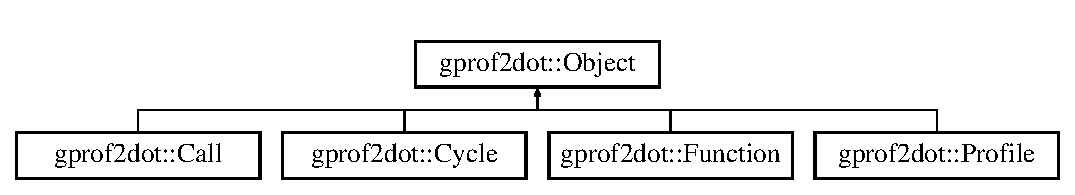
\includegraphics[height=2.000000cm]{classgprof2dot_1_1Object}
\end{center}
\end{figure}
\subsection*{Public Member Functions}
\begin{DoxyCompactItemize}
\item 
def \hyperlink{classgprof2dot_1_1Object_ae98eed8f428fdb899a83c5a659346c33}{\_\-\_\-init\_\-\_\-}
\item 
def \hyperlink{classgprof2dot_1_1Object_adbca16d1a1ee8ff2140e50f82fdd2485}{\_\-\_\-hash\_\-\_\-}
\item 
def \hyperlink{classgprof2dot_1_1Object_a7ff283c9ac1d0c8ab98d0c62a9e0c67d}{\_\-\_\-eq\_\-\_\-}
\item 
def \hyperlink{classgprof2dot_1_1Object_a3b944e8524a6ea4ea23eee28ad7e98d7}{\_\-\_\-contains\_\-\_\-}
\item 
def \hyperlink{classgprof2dot_1_1Object_a81b2078fb11399a1ae037aec45057167}{\_\-\_\-getitem\_\-\_\-}
\item 
def \hyperlink{classgprof2dot_1_1Object_a95da8c2aa46bb546fff598a3b2212ec3}{\_\-\_\-setitem\_\-\_\-}
\end{DoxyCompactItemize}
\subsection*{Public Attributes}
\begin{DoxyCompactItemize}
\item 
\hyperlink{classgprof2dot_1_1Object_a1361aa2a606f34d26b43fb87e0468680}{events}
\end{DoxyCompactItemize}


\subsection{Detailed Description}
\begin{DoxyVerb}Base class for all objects in profile which can store events.\end{DoxyVerb}
 

\subsection{Constructor \& Destructor Documentation}
\hypertarget{classgprof2dot_1_1Object_ae98eed8f428fdb899a83c5a659346c33}{
\index{gprof2dot::Object@{gprof2dot::Object}!\_\-\_\-init\_\-\_\-@{\_\-\_\-init\_\-\_\-}}
\index{\_\-\_\-init\_\-\_\-@{\_\-\_\-init\_\-\_\-}!gprof2dot::Object@{gprof2dot::Object}}
\subsubsection[{\_\-\_\-init\_\-\_\-}]{\setlength{\rightskip}{0pt plus 5cm}def gprof2dot::Object::\_\-\_\-init\_\-\_\- (
\begin{DoxyParamCaption}
\item[{}]{self, }
\item[{}]{events = {\ttfamily None}}
\end{DoxyParamCaption}
)}}
\label{classgprof2dot_1_1Object_ae98eed8f428fdb899a83c5a659346c33}


Reimplemented in \hyperlink{classgprof2dot_1_1Call_a2e6af456964a01d7fa4768224fbf729c}{gprof2dot::Call}.



\subsection{Member Function Documentation}
\hypertarget{classgprof2dot_1_1Object_a3b944e8524a6ea4ea23eee28ad7e98d7}{
\index{gprof2dot::Object@{gprof2dot::Object}!\_\-\_\-contains\_\-\_\-@{\_\-\_\-contains\_\-\_\-}}
\index{\_\-\_\-contains\_\-\_\-@{\_\-\_\-contains\_\-\_\-}!gprof2dot::Object@{gprof2dot::Object}}
\subsubsection[{\_\-\_\-contains\_\-\_\-}]{\setlength{\rightskip}{0pt plus 5cm}def gprof2dot::Object::\_\-\_\-contains\_\-\_\- (
\begin{DoxyParamCaption}
\item[{}]{self, }
\item[{}]{event}
\end{DoxyParamCaption}
)}}
\label{classgprof2dot_1_1Object_a3b944e8524a6ea4ea23eee28ad7e98d7}
\hypertarget{classgprof2dot_1_1Object_a7ff283c9ac1d0c8ab98d0c62a9e0c67d}{
\index{gprof2dot::Object@{gprof2dot::Object}!\_\-\_\-eq\_\-\_\-@{\_\-\_\-eq\_\-\_\-}}
\index{\_\-\_\-eq\_\-\_\-@{\_\-\_\-eq\_\-\_\-}!gprof2dot::Object@{gprof2dot::Object}}
\subsubsection[{\_\-\_\-eq\_\-\_\-}]{\setlength{\rightskip}{0pt plus 5cm}def gprof2dot::Object::\_\-\_\-eq\_\-\_\- (
\begin{DoxyParamCaption}
\item[{}]{self, }
\item[{}]{other}
\end{DoxyParamCaption}
)}}
\label{classgprof2dot_1_1Object_a7ff283c9ac1d0c8ab98d0c62a9e0c67d}
\hypertarget{classgprof2dot_1_1Object_a81b2078fb11399a1ae037aec45057167}{
\index{gprof2dot::Object@{gprof2dot::Object}!\_\-\_\-getitem\_\-\_\-@{\_\-\_\-getitem\_\-\_\-}}
\index{\_\-\_\-getitem\_\-\_\-@{\_\-\_\-getitem\_\-\_\-}!gprof2dot::Object@{gprof2dot::Object}}
\subsubsection[{\_\-\_\-getitem\_\-\_\-}]{\setlength{\rightskip}{0pt plus 5cm}def gprof2dot::Object::\_\-\_\-getitem\_\-\_\- (
\begin{DoxyParamCaption}
\item[{}]{self, }
\item[{}]{event}
\end{DoxyParamCaption}
)}}
\label{classgprof2dot_1_1Object_a81b2078fb11399a1ae037aec45057167}
\hypertarget{classgprof2dot_1_1Object_adbca16d1a1ee8ff2140e50f82fdd2485}{
\index{gprof2dot::Object@{gprof2dot::Object}!\_\-\_\-hash\_\-\_\-@{\_\-\_\-hash\_\-\_\-}}
\index{\_\-\_\-hash\_\-\_\-@{\_\-\_\-hash\_\-\_\-}!gprof2dot::Object@{gprof2dot::Object}}
\subsubsection[{\_\-\_\-hash\_\-\_\-}]{\setlength{\rightskip}{0pt plus 5cm}def gprof2dot::Object::\_\-\_\-hash\_\-\_\- (
\begin{DoxyParamCaption}
\item[{}]{self}
\end{DoxyParamCaption}
)}}
\label{classgprof2dot_1_1Object_adbca16d1a1ee8ff2140e50f82fdd2485}
\hypertarget{classgprof2dot_1_1Object_a95da8c2aa46bb546fff598a3b2212ec3}{
\index{gprof2dot::Object@{gprof2dot::Object}!\_\-\_\-setitem\_\-\_\-@{\_\-\_\-setitem\_\-\_\-}}
\index{\_\-\_\-setitem\_\-\_\-@{\_\-\_\-setitem\_\-\_\-}!gprof2dot::Object@{gprof2dot::Object}}
\subsubsection[{\_\-\_\-setitem\_\-\_\-}]{\setlength{\rightskip}{0pt plus 5cm}def gprof2dot::Object::\_\-\_\-setitem\_\-\_\- (
\begin{DoxyParamCaption}
\item[{}]{self, }
\item[{}]{event, }
\item[{}]{value}
\end{DoxyParamCaption}
)}}
\label{classgprof2dot_1_1Object_a95da8c2aa46bb546fff598a3b2212ec3}


\subsection{Member Data Documentation}
\hypertarget{classgprof2dot_1_1Object_a1361aa2a606f34d26b43fb87e0468680}{
\index{gprof2dot::Object@{gprof2dot::Object}!events@{events}}
\index{events@{events}!gprof2dot::Object@{gprof2dot::Object}}
\subsubsection[{events}]{\setlength{\rightskip}{0pt plus 5cm}{\bf gprof2dot::Object::events}}}
\label{classgprof2dot_1_1Object_a1361aa2a606f34d26b43fb87e0468680}


The documentation for this class was generated from the following file:\begin{DoxyCompactItemize}
\item 
\hyperlink{gprof2dot_8py}{gprof2dot.py}\end{DoxyCompactItemize}

\hypertarget{classgprof2dot_1_1OprofileParser}{
\section{gprof2dot::OprofileParser Class Reference}
\label{classgprof2dot_1_1OprofileParser}\index{gprof2dot::OprofileParser@{gprof2dot::OprofileParser}}
}
Inheritance diagram for gprof2dot::OprofileParser:\begin{figure}[H]
\begin{center}
\leavevmode
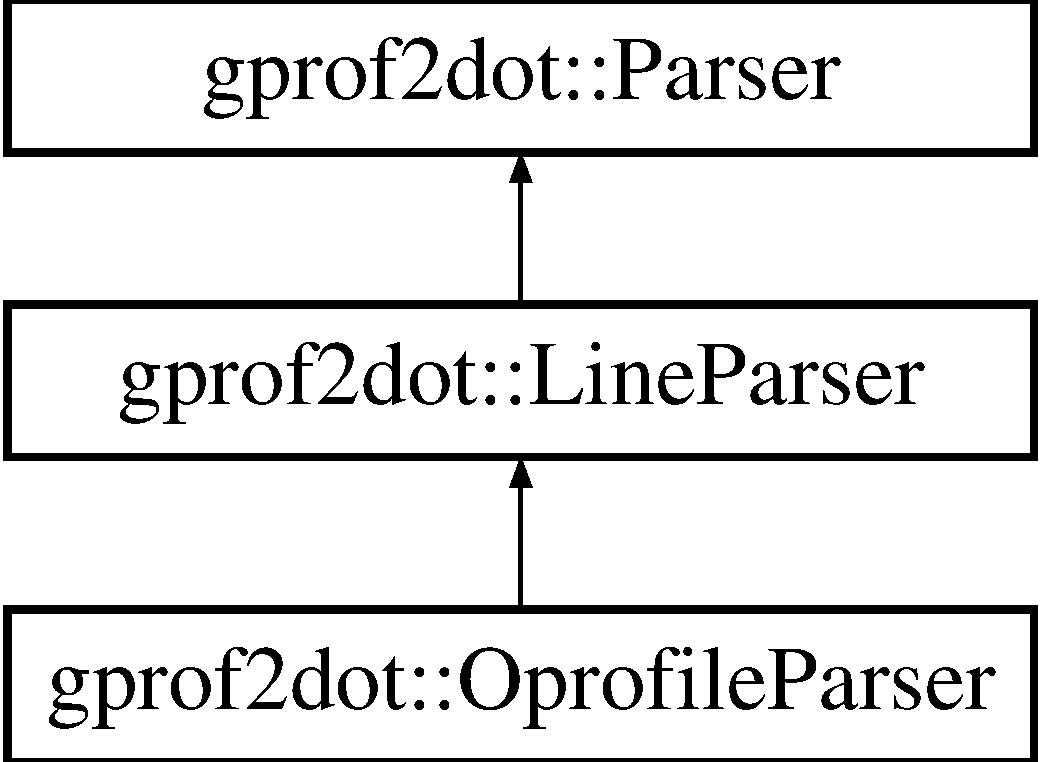
\includegraphics[height=3.000000cm]{classgprof2dot_1_1OprofileParser}
\end{center}
\end{figure}
\subsection*{Public Member Functions}
\begin{DoxyCompactItemize}
\item 
def \hyperlink{classgprof2dot_1_1OprofileParser_aae02e1a72d89b05709613913e176d115}{\_\-\_\-init\_\-\_\-}
\item 
def \hyperlink{classgprof2dot_1_1OprofileParser_a143e933d3fe4c53372597352aa08380c}{add\_\-entry}
\item 
def \hyperlink{classgprof2dot_1_1OprofileParser_a1409df50024a67e935a99a53e1ff0bbc}{update\_\-subentries\_\-dict}
\item 
def \hyperlink{classgprof2dot_1_1OprofileParser_a7dada0cbdc4a1514f17b3bca3189d5c8}{parse}
\item 
def \hyperlink{classgprof2dot_1_1OprofileParser_aa6ba17211a7774baeb7e41e0d4ce0948}{parse\_\-header}
\item 
def \hyperlink{classgprof2dot_1_1OprofileParser_a29c6f9d3e1a96c0437fca323f005a202}{parse\_\-entry}
\item 
def \hyperlink{classgprof2dot_1_1OprofileParser_ac3e0d08e198332b96b768f13e518399d}{parse\_\-subentries}
\item 
def \hyperlink{classgprof2dot_1_1OprofileParser_a9f3d0a641b6dba474b236dedd003142d}{parse\_\-subentry}
\item 
def \hyperlink{classgprof2dot_1_1OprofileParser_ae64ad152a018ee3c92e8c0f9cc4f11d3}{skip\_\-separator}
\item 
def \hyperlink{classgprof2dot_1_1OprofileParser_a69301f37fbcb8138b0dc9f2a8ed8149a}{match\_\-header}
\item 
def \hyperlink{classgprof2dot_1_1OprofileParser_a14b0bf734f26f60a30de6d2d3ff95f19}{match\_\-separator}
\item 
def \hyperlink{classgprof2dot_1_1OprofileParser_a4a7e21f9219f339a85a9d8526e387f84}{match\_\-primary}
\item 
def \hyperlink{classgprof2dot_1_1OprofileParser_a0a692d8bc590f7873142cd2cfb99f74f}{match\_\-secondary}
\end{DoxyCompactItemize}
\subsection*{Public Attributes}
\begin{DoxyCompactItemize}
\item 
\hyperlink{classgprof2dot_1_1OprofileParser_a49b07d5ed8e2c15fb8bdd85a0478e006}{entries}
\item 
\hyperlink{classgprof2dot_1_1OprofileParser_a486cc4eb05293a62bc1b8ef2fbc9ef56}{entry\_\-re}
\end{DoxyCompactItemize}


\subsection{Detailed Description}
\begin{DoxyVerb}Parser for oprofile callgraph output.

See also:
- http://oprofile.sourceforge.net/doc/opreport.html#opreport-callgraph
\end{DoxyVerb}
 

\subsection{Constructor \& Destructor Documentation}
\hypertarget{classgprof2dot_1_1OprofileParser_aae02e1a72d89b05709613913e176d115}{
\index{gprof2dot::OprofileParser@{gprof2dot::OprofileParser}!\_\-\_\-init\_\-\_\-@{\_\-\_\-init\_\-\_\-}}
\index{\_\-\_\-init\_\-\_\-@{\_\-\_\-init\_\-\_\-}!gprof2dot::OprofileParser@{gprof2dot::OprofileParser}}
\subsubsection[{\_\-\_\-init\_\-\_\-}]{\setlength{\rightskip}{0pt plus 5cm}def gprof2dot::OprofileParser::\_\-\_\-init\_\-\_\- (
\begin{DoxyParamCaption}
\item[{}]{self, }
\item[{}]{infile}
\end{DoxyParamCaption}
)}}
\label{classgprof2dot_1_1OprofileParser_aae02e1a72d89b05709613913e176d115}


Reimplemented from \hyperlink{classgprof2dot_1_1LineParser_a9ab24f364f64a70181dd4156cea194c5}{gprof2dot::LineParser}.



\subsection{Member Function Documentation}
\hypertarget{classgprof2dot_1_1OprofileParser_a143e933d3fe4c53372597352aa08380c}{
\index{gprof2dot::OprofileParser@{gprof2dot::OprofileParser}!add\_\-entry@{add\_\-entry}}
\index{add\_\-entry@{add\_\-entry}!gprof2dot::OprofileParser@{gprof2dot::OprofileParser}}
\subsubsection[{add\_\-entry}]{\setlength{\rightskip}{0pt plus 5cm}def gprof2dot::OprofileParser::add\_\-entry (
\begin{DoxyParamCaption}
\item[{}]{self, }
\item[{}]{callers, }
\item[{}]{function, }
\item[{}]{callees}
\end{DoxyParamCaption}
)}}
\label{classgprof2dot_1_1OprofileParser_a143e933d3fe4c53372597352aa08380c}
\hypertarget{classgprof2dot_1_1OprofileParser_a69301f37fbcb8138b0dc9f2a8ed8149a}{
\index{gprof2dot::OprofileParser@{gprof2dot::OprofileParser}!match\_\-header@{match\_\-header}}
\index{match\_\-header@{match\_\-header}!gprof2dot::OprofileParser@{gprof2dot::OprofileParser}}
\subsubsection[{match\_\-header}]{\setlength{\rightskip}{0pt plus 5cm}def gprof2dot::OprofileParser::match\_\-header (
\begin{DoxyParamCaption}
\item[{}]{self}
\end{DoxyParamCaption}
)}}
\label{classgprof2dot_1_1OprofileParser_a69301f37fbcb8138b0dc9f2a8ed8149a}
\hypertarget{classgprof2dot_1_1OprofileParser_a4a7e21f9219f339a85a9d8526e387f84}{
\index{gprof2dot::OprofileParser@{gprof2dot::OprofileParser}!match\_\-primary@{match\_\-primary}}
\index{match\_\-primary@{match\_\-primary}!gprof2dot::OprofileParser@{gprof2dot::OprofileParser}}
\subsubsection[{match\_\-primary}]{\setlength{\rightskip}{0pt plus 5cm}def gprof2dot::OprofileParser::match\_\-primary (
\begin{DoxyParamCaption}
\item[{}]{self}
\end{DoxyParamCaption}
)}}
\label{classgprof2dot_1_1OprofileParser_a4a7e21f9219f339a85a9d8526e387f84}
\hypertarget{classgprof2dot_1_1OprofileParser_a0a692d8bc590f7873142cd2cfb99f74f}{
\index{gprof2dot::OprofileParser@{gprof2dot::OprofileParser}!match\_\-secondary@{match\_\-secondary}}
\index{match\_\-secondary@{match\_\-secondary}!gprof2dot::OprofileParser@{gprof2dot::OprofileParser}}
\subsubsection[{match\_\-secondary}]{\setlength{\rightskip}{0pt plus 5cm}def gprof2dot::OprofileParser::match\_\-secondary (
\begin{DoxyParamCaption}
\item[{}]{self}
\end{DoxyParamCaption}
)}}
\label{classgprof2dot_1_1OprofileParser_a0a692d8bc590f7873142cd2cfb99f74f}
\hypertarget{classgprof2dot_1_1OprofileParser_a14b0bf734f26f60a30de6d2d3ff95f19}{
\index{gprof2dot::OprofileParser@{gprof2dot::OprofileParser}!match\_\-separator@{match\_\-separator}}
\index{match\_\-separator@{match\_\-separator}!gprof2dot::OprofileParser@{gprof2dot::OprofileParser}}
\subsubsection[{match\_\-separator}]{\setlength{\rightskip}{0pt plus 5cm}def gprof2dot::OprofileParser::match\_\-separator (
\begin{DoxyParamCaption}
\item[{}]{self}
\end{DoxyParamCaption}
)}}
\label{classgprof2dot_1_1OprofileParser_a14b0bf734f26f60a30de6d2d3ff95f19}
\hypertarget{classgprof2dot_1_1OprofileParser_a7dada0cbdc4a1514f17b3bca3189d5c8}{
\index{gprof2dot::OprofileParser@{gprof2dot::OprofileParser}!parse@{parse}}
\index{parse@{parse}!gprof2dot::OprofileParser@{gprof2dot::OprofileParser}}
\subsubsection[{parse}]{\setlength{\rightskip}{0pt plus 5cm}def gprof2dot::OprofileParser::parse (
\begin{DoxyParamCaption}
\item[{}]{self}
\end{DoxyParamCaption}
)}}
\label{classgprof2dot_1_1OprofileParser_a7dada0cbdc4a1514f17b3bca3189d5c8}


Reimplemented from \hyperlink{classgprof2dot_1_1Parser_a681a0bc74e640c9c8e3d629dd03049fc}{gprof2dot::Parser}.

\hypertarget{classgprof2dot_1_1OprofileParser_a29c6f9d3e1a96c0437fca323f005a202}{
\index{gprof2dot::OprofileParser@{gprof2dot::OprofileParser}!parse\_\-entry@{parse\_\-entry}}
\index{parse\_\-entry@{parse\_\-entry}!gprof2dot::OprofileParser@{gprof2dot::OprofileParser}}
\subsubsection[{parse\_\-entry}]{\setlength{\rightskip}{0pt plus 5cm}def gprof2dot::OprofileParser::parse\_\-entry (
\begin{DoxyParamCaption}
\item[{}]{self}
\end{DoxyParamCaption}
)}}
\label{classgprof2dot_1_1OprofileParser_a29c6f9d3e1a96c0437fca323f005a202}
\hypertarget{classgprof2dot_1_1OprofileParser_aa6ba17211a7774baeb7e41e0d4ce0948}{
\index{gprof2dot::OprofileParser@{gprof2dot::OprofileParser}!parse\_\-header@{parse\_\-header}}
\index{parse\_\-header@{parse\_\-header}!gprof2dot::OprofileParser@{gprof2dot::OprofileParser}}
\subsubsection[{parse\_\-header}]{\setlength{\rightskip}{0pt plus 5cm}def gprof2dot::OprofileParser::parse\_\-header (
\begin{DoxyParamCaption}
\item[{}]{self}
\end{DoxyParamCaption}
)}}
\label{classgprof2dot_1_1OprofileParser_aa6ba17211a7774baeb7e41e0d4ce0948}
\hypertarget{classgprof2dot_1_1OprofileParser_ac3e0d08e198332b96b768f13e518399d}{
\index{gprof2dot::OprofileParser@{gprof2dot::OprofileParser}!parse\_\-subentries@{parse\_\-subentries}}
\index{parse\_\-subentries@{parse\_\-subentries}!gprof2dot::OprofileParser@{gprof2dot::OprofileParser}}
\subsubsection[{parse\_\-subentries}]{\setlength{\rightskip}{0pt plus 5cm}def gprof2dot::OprofileParser::parse\_\-subentries (
\begin{DoxyParamCaption}
\item[{}]{self}
\end{DoxyParamCaption}
)}}
\label{classgprof2dot_1_1OprofileParser_ac3e0d08e198332b96b768f13e518399d}
\hypertarget{classgprof2dot_1_1OprofileParser_a9f3d0a641b6dba474b236dedd003142d}{
\index{gprof2dot::OprofileParser@{gprof2dot::OprofileParser}!parse\_\-subentry@{parse\_\-subentry}}
\index{parse\_\-subentry@{parse\_\-subentry}!gprof2dot::OprofileParser@{gprof2dot::OprofileParser}}
\subsubsection[{parse\_\-subentry}]{\setlength{\rightskip}{0pt plus 5cm}def gprof2dot::OprofileParser::parse\_\-subentry (
\begin{DoxyParamCaption}
\item[{}]{self}
\end{DoxyParamCaption}
)}}
\label{classgprof2dot_1_1OprofileParser_a9f3d0a641b6dba474b236dedd003142d}
\hypertarget{classgprof2dot_1_1OprofileParser_ae64ad152a018ee3c92e8c0f9cc4f11d3}{
\index{gprof2dot::OprofileParser@{gprof2dot::OprofileParser}!skip\_\-separator@{skip\_\-separator}}
\index{skip\_\-separator@{skip\_\-separator}!gprof2dot::OprofileParser@{gprof2dot::OprofileParser}}
\subsubsection[{skip\_\-separator}]{\setlength{\rightskip}{0pt plus 5cm}def gprof2dot::OprofileParser::skip\_\-separator (
\begin{DoxyParamCaption}
\item[{}]{self}
\end{DoxyParamCaption}
)}}
\label{classgprof2dot_1_1OprofileParser_ae64ad152a018ee3c92e8c0f9cc4f11d3}
\hypertarget{classgprof2dot_1_1OprofileParser_a1409df50024a67e935a99a53e1ff0bbc}{
\index{gprof2dot::OprofileParser@{gprof2dot::OprofileParser}!update\_\-subentries\_\-dict@{update\_\-subentries\_\-dict}}
\index{update\_\-subentries\_\-dict@{update\_\-subentries\_\-dict}!gprof2dot::OprofileParser@{gprof2dot::OprofileParser}}
\subsubsection[{update\_\-subentries\_\-dict}]{\setlength{\rightskip}{0pt plus 5cm}def gprof2dot::OprofileParser::update\_\-subentries\_\-dict (
\begin{DoxyParamCaption}
\item[{}]{self, }
\item[{}]{totals, }
\item[{}]{partials}
\end{DoxyParamCaption}
)}}
\label{classgprof2dot_1_1OprofileParser_a1409df50024a67e935a99a53e1ff0bbc}


\subsection{Member Data Documentation}
\hypertarget{classgprof2dot_1_1OprofileParser_a49b07d5ed8e2c15fb8bdd85a0478e006}{
\index{gprof2dot::OprofileParser@{gprof2dot::OprofileParser}!entries@{entries}}
\index{entries@{entries}!gprof2dot::OprofileParser@{gprof2dot::OprofileParser}}
\subsubsection[{entries}]{\setlength{\rightskip}{0pt plus 5cm}{\bf gprof2dot::OprofileParser::entries}}}
\label{classgprof2dot_1_1OprofileParser_a49b07d5ed8e2c15fb8bdd85a0478e006}
\hypertarget{classgprof2dot_1_1OprofileParser_a486cc4eb05293a62bc1b8ef2fbc9ef56}{
\index{gprof2dot::OprofileParser@{gprof2dot::OprofileParser}!entry\_\-re@{entry\_\-re}}
\index{entry\_\-re@{entry\_\-re}!gprof2dot::OprofileParser@{gprof2dot::OprofileParser}}
\subsubsection[{entry\_\-re}]{\setlength{\rightskip}{0pt plus 5cm}{\bf gprof2dot::OprofileParser::entry\_\-re}}}
\label{classgprof2dot_1_1OprofileParser_a486cc4eb05293a62bc1b8ef2fbc9ef56}


The documentation for this class was generated from the following file:\begin{DoxyCompactItemize}
\item 
\hyperlink{gprof2dot_8py}{gprof2dot.py}\end{DoxyCompactItemize}

\hypertarget{classgprof2dot_1_1ParseError}{
\section{gprof2dot::ParseError Class Reference}
\label{classgprof2dot_1_1ParseError}\index{gprof2dot::ParseError@{gprof2dot::ParseError}}
}
\subsection*{Public Member Functions}
\begin{DoxyCompactItemize}
\item 
def \hyperlink{classgprof2dot_1_1ParseError_af8f7b8f57d070f8e85bcfb415b859beb}{\_\-\_\-init\_\-\_\-}
\item 
def \hyperlink{classgprof2dot_1_1ParseError_af6645cc79dee41ff44612ece0770a76e}{\_\-\_\-str\_\-\_\-}
\end{DoxyCompactItemize}
\subsection*{Public Attributes}
\begin{DoxyCompactItemize}
\item 
\hyperlink{classgprof2dot_1_1ParseError_afc238352cf8722a3b53b71d637274c62}{msg}
\item 
\hyperlink{classgprof2dot_1_1ParseError_ab6c0c009b99780885685ac1c0ab9d5f7}{line}
\end{DoxyCompactItemize}


\subsection{Detailed Description}
\begin{DoxyVerb}Raised when parsing to signal mismatches.\end{DoxyVerb}
 

\subsection{Constructor \& Destructor Documentation}
\hypertarget{classgprof2dot_1_1ParseError_af8f7b8f57d070f8e85bcfb415b859beb}{
\index{gprof2dot::ParseError@{gprof2dot::ParseError}!\_\-\_\-init\_\-\_\-@{\_\-\_\-init\_\-\_\-}}
\index{\_\-\_\-init\_\-\_\-@{\_\-\_\-init\_\-\_\-}!gprof2dot::ParseError@{gprof2dot::ParseError}}
\subsubsection[{\_\-\_\-init\_\-\_\-}]{\setlength{\rightskip}{0pt plus 5cm}def gprof2dot::ParseError::\_\-\_\-init\_\-\_\- (
\begin{DoxyParamCaption}
\item[{}]{self, }
\item[{}]{msg, }
\item[{}]{line}
\end{DoxyParamCaption}
)}}
\label{classgprof2dot_1_1ParseError_af8f7b8f57d070f8e85bcfb415b859beb}


\subsection{Member Function Documentation}
\hypertarget{classgprof2dot_1_1ParseError_af6645cc79dee41ff44612ece0770a76e}{
\index{gprof2dot::ParseError@{gprof2dot::ParseError}!\_\-\_\-str\_\-\_\-@{\_\-\_\-str\_\-\_\-}}
\index{\_\-\_\-str\_\-\_\-@{\_\-\_\-str\_\-\_\-}!gprof2dot::ParseError@{gprof2dot::ParseError}}
\subsubsection[{\_\-\_\-str\_\-\_\-}]{\setlength{\rightskip}{0pt plus 5cm}def gprof2dot::ParseError::\_\-\_\-str\_\-\_\- (
\begin{DoxyParamCaption}
\item[{}]{self}
\end{DoxyParamCaption}
)}}
\label{classgprof2dot_1_1ParseError_af6645cc79dee41ff44612ece0770a76e}


\subsection{Member Data Documentation}
\hypertarget{classgprof2dot_1_1ParseError_ab6c0c009b99780885685ac1c0ab9d5f7}{
\index{gprof2dot::ParseError@{gprof2dot::ParseError}!line@{line}}
\index{line@{line}!gprof2dot::ParseError@{gprof2dot::ParseError}}
\subsubsection[{line}]{\setlength{\rightskip}{0pt plus 5cm}{\bf gprof2dot::ParseError::line}}}
\label{classgprof2dot_1_1ParseError_ab6c0c009b99780885685ac1c0ab9d5f7}
\hypertarget{classgprof2dot_1_1ParseError_afc238352cf8722a3b53b71d637274c62}{
\index{gprof2dot::ParseError@{gprof2dot::ParseError}!msg@{msg}}
\index{msg@{msg}!gprof2dot::ParseError@{gprof2dot::ParseError}}
\subsubsection[{msg}]{\setlength{\rightskip}{0pt plus 5cm}{\bf gprof2dot::ParseError::msg}}}
\label{classgprof2dot_1_1ParseError_afc238352cf8722a3b53b71d637274c62}


The documentation for this class was generated from the following file:\begin{DoxyCompactItemize}
\item 
\hyperlink{gprof2dot_8py}{gprof2dot.py}\end{DoxyCompactItemize}

\hypertarget{classParser}{
\section{Parser Class Reference}
\label{classParser}\index{Parser@{Parser}}
}


Utilizado para converter a entrada do usuario em uma \hyperlink{classCommandLine}{CommandLine}.  




{\ttfamily \#include $<$Parser.hpp$>$}

\subsection*{Public Member Functions}
\begin{DoxyCompactItemize}
\item 
\hyperlink{classParser_a12234f6cd36b61af4b50c94a179422c1}{Parser} ()
\item 
\hyperlink{classCommandLine}{CommandLine} $\ast$ \hyperlink{classParser_a992f6612be5ab4a587e29c7ed5c824c3}{readCommandLine} ()
\item 
bool \hyperlink{classParser_a2d6e80902c93ceed3d8f9a2f7cacd50c}{newLine} ()
\end{DoxyCompactItemize}


\subsection{Detailed Description}
Utilizado para converter a entrada do usuario em uma \hyperlink{classCommandLine}{CommandLine}. A linha de usuario deve ter a seguinte forma\par
 $<$comando$>$$<$paramentro$>$...$<$parametro$>$$|$...$|$$<$comando$>$...\mbox{[}$<$ $<$entrada$>$\mbox{]}\mbox{[}\mbox{[}1$>$$|$$>$$|$$>$$>$\mbox{]}\mbox{[}2$>$\mbox{]}$<$saida$>$$|$\&$>$$<$saida$>$\mbox{]}\mbox{[}\&\mbox{]} 

\subsection{Constructor \& Destructor Documentation}
\hypertarget{classParser_a12234f6cd36b61af4b50c94a179422c1}{
\index{Parser@{Parser}!Parser@{Parser}}
\index{Parser@{Parser}!Parser@{Parser}}
\subsubsection[{Parser}]{\setlength{\rightskip}{0pt plus 5cm}Parser::Parser (
\begin{DoxyParamCaption}
{}
\end{DoxyParamCaption}
)}}
\label{classParser_a12234f6cd36b61af4b50c94a179422c1}


\subsection{Member Function Documentation}
\hypertarget{classParser_a2d6e80902c93ceed3d8f9a2f7cacd50c}{
\index{Parser@{Parser}!newLine@{newLine}}
\index{newLine@{newLine}!Parser@{Parser}}
\subsubsection[{newLine}]{\setlength{\rightskip}{0pt plus 5cm}bool Parser::newLine (
\begin{DoxyParamCaption}
{}
\end{DoxyParamCaption}
)}}
\label{classParser_a2d6e80902c93ceed3d8f9a2f7cacd50c}
\begin{DoxyReturn}{Returns}
Verdadeiro caso esteja em uma nova linha de comando (nao necessariamente endl, mas fim da pipeline por \& 
\end{DoxyReturn}
\hypertarget{classParser_a992f6612be5ab4a587e29c7ed5c824c3}{
\index{Parser@{Parser}!readCommandLine@{readCommandLine}}
\index{readCommandLine@{readCommandLine}!Parser@{Parser}}
\subsubsection[{readCommandLine}]{\setlength{\rightskip}{0pt plus 5cm}{\bf CommandLine} $\ast$ Parser::readCommandLine (
\begin{DoxyParamCaption}
{}
\end{DoxyParamCaption}
)}}
\label{classParser_a992f6612be5ab4a587e29c7ed5c824c3}
\begin{DoxyReturn}{Returns}
Le e interpreta uma linha de comando dada pelo usuario no stdin 
\end{DoxyReturn}


The documentation for this class was generated from the following files:\begin{DoxyCompactItemize}
\item 
\hyperlink{Parser_8hpp}{Parser.hpp}\item 
\hyperlink{Parser_8cpp}{Parser.cpp}\end{DoxyCompactItemize}

\hypertarget{classgprof2dot_1_1Parser}{
\section{gprof2dot::Parser Class Reference}
\label{classgprof2dot_1_1Parser}\index{gprof2dot::Parser@{gprof2dot::Parser}}
}
Inheritance diagram for gprof2dot::Parser:\begin{figure}[H]
\begin{center}
\leavevmode
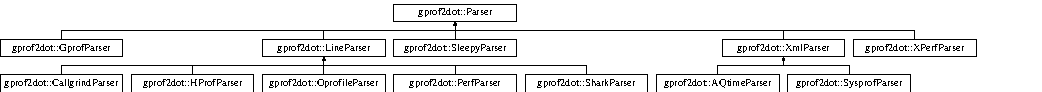
\includegraphics[height=1.242604cm]{classgprof2dot_1_1Parser}
\end{center}
\end{figure}
\subsection*{Public Member Functions}
\begin{DoxyCompactItemize}
\item 
def \hyperlink{classgprof2dot_1_1Parser_a0041897b2ea4f3cb61c7c16b351c2c5a}{\_\-\_\-init\_\-\_\-}
\item 
def \hyperlink{classgprof2dot_1_1Parser_a681a0bc74e640c9c8e3d629dd03049fc}{parse}
\end{DoxyCompactItemize}


\subsection{Detailed Description}
\begin{DoxyVerb}Parser interface.\end{DoxyVerb}
 

\subsection{Constructor \& Destructor Documentation}
\hypertarget{classgprof2dot_1_1Parser_a0041897b2ea4f3cb61c7c16b351c2c5a}{
\index{gprof2dot::Parser@{gprof2dot::Parser}!\_\-\_\-init\_\-\_\-@{\_\-\_\-init\_\-\_\-}}
\index{\_\-\_\-init\_\-\_\-@{\_\-\_\-init\_\-\_\-}!gprof2dot::Parser@{gprof2dot::Parser}}
\subsubsection[{\_\-\_\-init\_\-\_\-}]{\setlength{\rightskip}{0pt plus 5cm}def gprof2dot::Parser::\_\-\_\-init\_\-\_\- (
\begin{DoxyParamCaption}
\item[{}]{self}
\end{DoxyParamCaption}
)}}
\label{classgprof2dot_1_1Parser_a0041897b2ea4f3cb61c7c16b351c2c5a}


\subsection{Member Function Documentation}
\hypertarget{classgprof2dot_1_1Parser_a681a0bc74e640c9c8e3d629dd03049fc}{
\index{gprof2dot::Parser@{gprof2dot::Parser}!parse@{parse}}
\index{parse@{parse}!gprof2dot::Parser@{gprof2dot::Parser}}
\subsubsection[{parse}]{\setlength{\rightskip}{0pt plus 5cm}def gprof2dot::Parser::parse (
\begin{DoxyParamCaption}
\item[{}]{self}
\end{DoxyParamCaption}
)}}
\label{classgprof2dot_1_1Parser_a681a0bc74e640c9c8e3d629dd03049fc}


Reimplemented in \hyperlink{classgprof2dot_1_1GprofParser_a840c96752592fffdb69514cf59022705}{gprof2dot::GprofParser}, \hyperlink{classgprof2dot_1_1CallgrindParser_ad5ef0ee6f7e2c0987f49452ef1488ea0}{gprof2dot::CallgrindParser}, \hyperlink{classgprof2dot_1_1PerfParser_a29992f3ede194162b1403a541cfe66ed}{gprof2dot::PerfParser}, \hyperlink{classgprof2dot_1_1OprofileParser_a7dada0cbdc4a1514f17b3bca3189d5c8}{gprof2dot::OprofileParser}, \hyperlink{classgprof2dot_1_1HProfParser_a8f6dc9e1899c27794ccc8676a33d62fa}{gprof2dot::HProfParser}, \hyperlink{classgprof2dot_1_1SysprofParser_acee5f7e208dd8f8d6ed73b88a70f2e7b}{gprof2dot::SysprofParser}, \hyperlink{classgprof2dot_1_1SharkParser_a50aedd037118d47393d3c8afe915be75}{gprof2dot::SharkParser}, \hyperlink{classgprof2dot_1_1XPerfParser_ac98402f482a2413c430558a01f51a75d}{gprof2dot::XPerfParser}, and \hyperlink{classgprof2dot_1_1AQtimeParser_ab1e9b6f7ddff3943366aba840235aa87}{gprof2dot::AQtimeParser}.



The documentation for this class was generated from the following file:\begin{DoxyCompactItemize}
\item 
\hyperlink{gprof2dot_8py}{gprof2dot.py}\end{DoxyCompactItemize}

\hypertarget{classgprof2dot_1_1PerfParser}{
\section{gprof2dot::PerfParser Class Reference}
\label{classgprof2dot_1_1PerfParser}\index{gprof2dot::PerfParser@{gprof2dot::PerfParser}}
}
Inheritance diagram for gprof2dot::PerfParser:\begin{figure}[H]
\begin{center}
\leavevmode
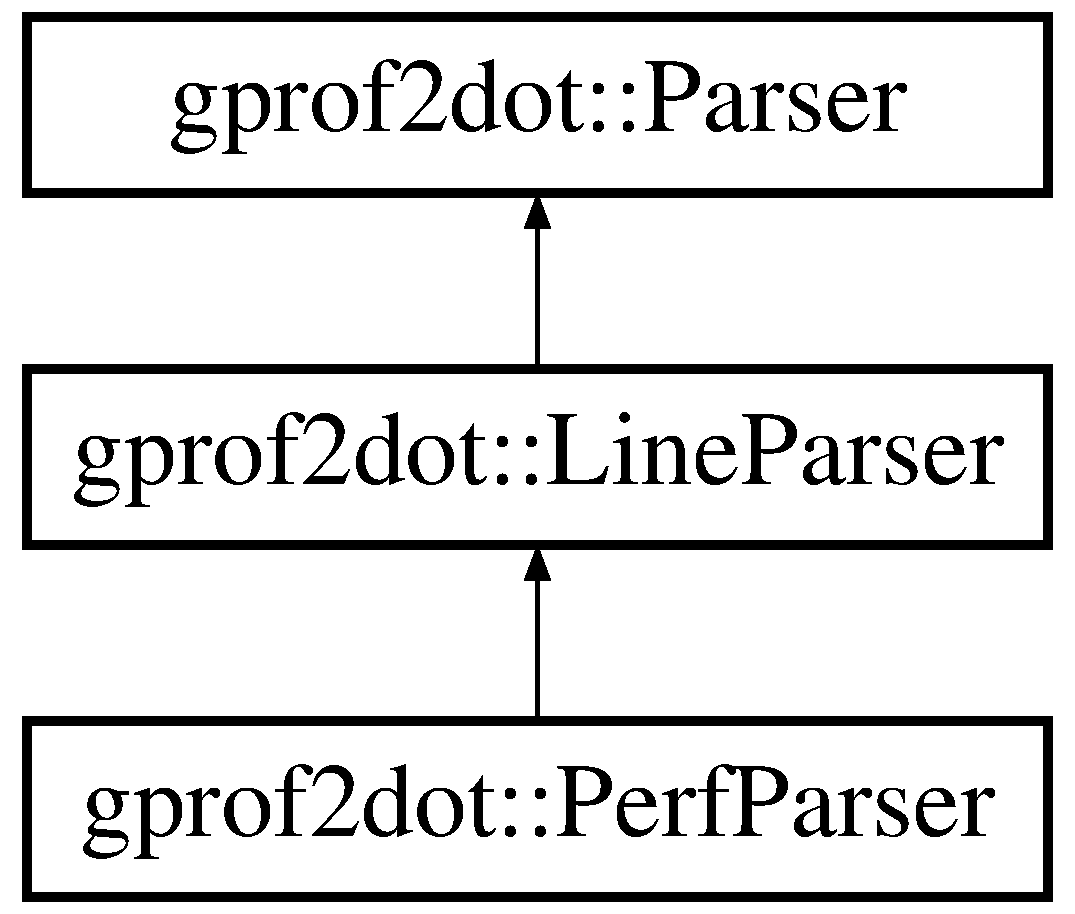
\includegraphics[height=3.000000cm]{classgprof2dot_1_1PerfParser}
\end{center}
\end{figure}
\subsection*{Public Member Functions}
\begin{DoxyCompactItemize}
\item 
def \hyperlink{classgprof2dot_1_1PerfParser_ad9a8aceb6ddebf85cb4814717a33e36f}{\_\-\_\-init\_\-\_\-}
\item 
def \hyperlink{classgprof2dot_1_1PerfParser_a29992f3ede194162b1403a541cfe66ed}{parse}
\item 
def \hyperlink{classgprof2dot_1_1PerfParser_a9dbfb8569cfb56cfa239a7607d742f9b}{parse\_\-event}
\item 
def \hyperlink{classgprof2dot_1_1PerfParser_a4c365c45b730a63ab9e563a297cefb05}{parse\_\-callchain}
\end{DoxyCompactItemize}
\subsection*{Public Attributes}
\begin{DoxyCompactItemize}
\item 
\hyperlink{classgprof2dot_1_1PerfParser_a43e50a541198b068aa4d4d2bfb5d3ea0}{profile}
\end{DoxyCompactItemize}
\subsection*{Static Public Attributes}
\begin{DoxyCompactItemize}
\item 
tuple \hyperlink{classgprof2dot_1_1PerfParser_a4d233c4bf5eade9c8e39234afe4a0ff2}{call\_\-re} = re.compile(r'$^\wedge$$\backslash$s+(?P$<$address$>$\mbox{[}0-\/9a-\/fA-\/F\mbox{]}+)$\backslash$s+(?P$<$symbol$>$.$\ast$)$\backslash$s+$\backslash$((?P$<$module$>$\mbox{[}$^\wedge$)\mbox{]}$\ast$)$\backslash$)
\end{DoxyCompactItemize}


\subsection{Detailed Description}
\begin{DoxyVerb}Parser for linux perf callgraph output.

It expects output generated with

    perf record -g
    perf script | gprof2dot.py --format=perf
\end{DoxyVerb}
 

\subsection{Constructor \& Destructor Documentation}
\hypertarget{classgprof2dot_1_1PerfParser_ad9a8aceb6ddebf85cb4814717a33e36f}{
\index{gprof2dot::PerfParser@{gprof2dot::PerfParser}!\_\-\_\-init\_\-\_\-@{\_\-\_\-init\_\-\_\-}}
\index{\_\-\_\-init\_\-\_\-@{\_\-\_\-init\_\-\_\-}!gprof2dot::PerfParser@{gprof2dot::PerfParser}}
\subsubsection[{\_\-\_\-init\_\-\_\-}]{\setlength{\rightskip}{0pt plus 5cm}def gprof2dot::PerfParser::\_\-\_\-init\_\-\_\- (
\begin{DoxyParamCaption}
\item[{}]{self, }
\item[{}]{infile}
\end{DoxyParamCaption}
)}}
\label{classgprof2dot_1_1PerfParser_ad9a8aceb6ddebf85cb4814717a33e36f}


Reimplemented from \hyperlink{classgprof2dot_1_1LineParser_a9ab24f364f64a70181dd4156cea194c5}{gprof2dot::LineParser}.



\subsection{Member Function Documentation}
\hypertarget{classgprof2dot_1_1PerfParser_a29992f3ede194162b1403a541cfe66ed}{
\index{gprof2dot::PerfParser@{gprof2dot::PerfParser}!parse@{parse}}
\index{parse@{parse}!gprof2dot::PerfParser@{gprof2dot::PerfParser}}
\subsubsection[{parse}]{\setlength{\rightskip}{0pt plus 5cm}def gprof2dot::PerfParser::parse (
\begin{DoxyParamCaption}
\item[{}]{self}
\end{DoxyParamCaption}
)}}
\label{classgprof2dot_1_1PerfParser_a29992f3ede194162b1403a541cfe66ed}


Reimplemented from \hyperlink{classgprof2dot_1_1Parser_a681a0bc74e640c9c8e3d629dd03049fc}{gprof2dot::Parser}.

\hypertarget{classgprof2dot_1_1PerfParser_a4c365c45b730a63ab9e563a297cefb05}{
\index{gprof2dot::PerfParser@{gprof2dot::PerfParser}!parse\_\-callchain@{parse\_\-callchain}}
\index{parse\_\-callchain@{parse\_\-callchain}!gprof2dot::PerfParser@{gprof2dot::PerfParser}}
\subsubsection[{parse\_\-callchain}]{\setlength{\rightskip}{0pt plus 5cm}def gprof2dot::PerfParser::parse\_\-callchain (
\begin{DoxyParamCaption}
\item[{}]{self}
\end{DoxyParamCaption}
)}}
\label{classgprof2dot_1_1PerfParser_a4c365c45b730a63ab9e563a297cefb05}
\hypertarget{classgprof2dot_1_1PerfParser_a9dbfb8569cfb56cfa239a7607d742f9b}{
\index{gprof2dot::PerfParser@{gprof2dot::PerfParser}!parse\_\-event@{parse\_\-event}}
\index{parse\_\-event@{parse\_\-event}!gprof2dot::PerfParser@{gprof2dot::PerfParser}}
\subsubsection[{parse\_\-event}]{\setlength{\rightskip}{0pt plus 5cm}def gprof2dot::PerfParser::parse\_\-event (
\begin{DoxyParamCaption}
\item[{}]{self}
\end{DoxyParamCaption}
)}}
\label{classgprof2dot_1_1PerfParser_a9dbfb8569cfb56cfa239a7607d742f9b}


\subsection{Member Data Documentation}
\hypertarget{classgprof2dot_1_1PerfParser_a4d233c4bf5eade9c8e39234afe4a0ff2}{
\index{gprof2dot::PerfParser@{gprof2dot::PerfParser}!call\_\-re@{call\_\-re}}
\index{call\_\-re@{call\_\-re}!gprof2dot::PerfParser@{gprof2dot::PerfParser}}
\subsubsection[{call\_\-re}]{\setlength{\rightskip}{0pt plus 5cm}tuple {\bf gprof2dot::PerfParser::call\_\-re} = re.compile(r'$^\wedge$$\backslash$s+(?P$<$address$>$\mbox{[}0-\/9a-\/fA-\/F\mbox{]}+)$\backslash$s+(?P$<$symbol$>$.$\ast$)$\backslash$s+$\backslash$((?P$<$module$>$\mbox{[}$^\wedge$)\mbox{]}$\ast$)$\backslash$)\hspace{0.3cm}{\ttfamily  \mbox{[}static\mbox{]}}}}
\label{classgprof2dot_1_1PerfParser_a4d233c4bf5eade9c8e39234afe4a0ff2}
\hypertarget{classgprof2dot_1_1PerfParser_a43e50a541198b068aa4d4d2bfb5d3ea0}{
\index{gprof2dot::PerfParser@{gprof2dot::PerfParser}!profile@{profile}}
\index{profile@{profile}!gprof2dot::PerfParser@{gprof2dot::PerfParser}}
\subsubsection[{profile}]{\setlength{\rightskip}{0pt plus 5cm}{\bf gprof2dot::PerfParser::profile}}}
\label{classgprof2dot_1_1PerfParser_a43e50a541198b068aa4d4d2bfb5d3ea0}


The documentation for this class was generated from the following file:\begin{DoxyCompactItemize}
\item 
\hyperlink{gprof2dot_8py}{gprof2dot.py}\end{DoxyCompactItemize}

\hypertarget{classgprof2dot_1_1Profile}{
\section{gprof2dot::Profile Class Reference}
\label{classgprof2dot_1_1Profile}\index{gprof2dot::Profile@{gprof2dot::Profile}}
}
Inheritance diagram for gprof2dot::Profile:\begin{figure}[H]
\begin{center}
\leavevmode
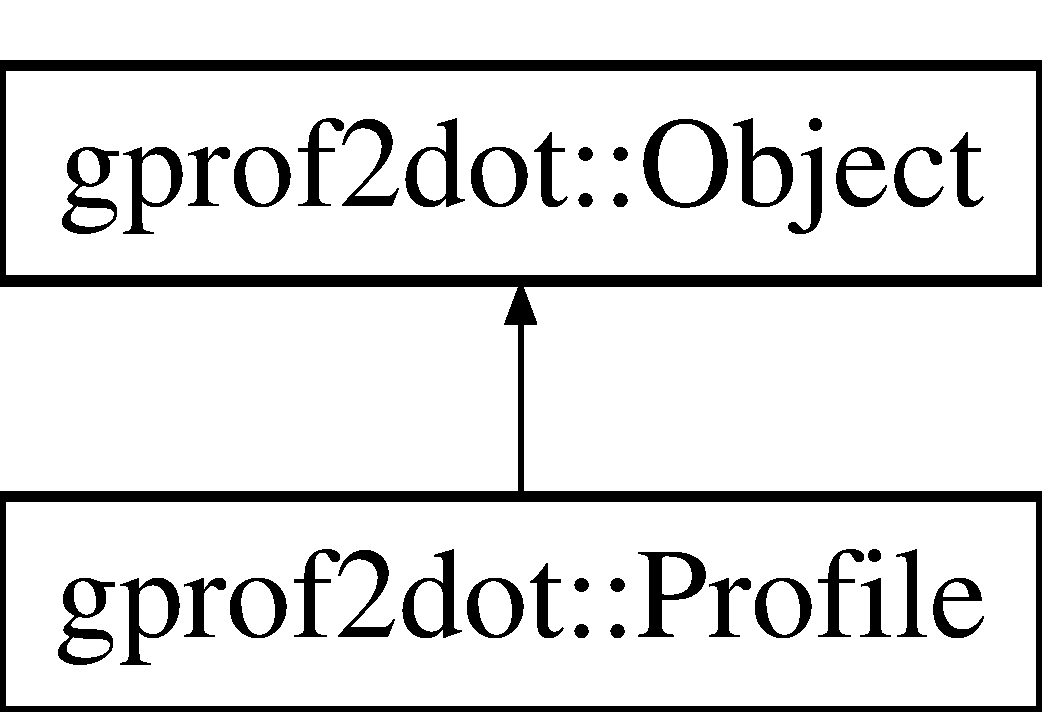
\includegraphics[height=2.000000cm]{classgprof2dot_1_1Profile}
\end{center}
\end{figure}
\subsection*{Public Member Functions}
\begin{DoxyCompactItemize}
\item 
def \hyperlink{classgprof2dot_1_1Profile_a382a908aa54d329efa5a665de49b6913}{\_\-\_\-init\_\-\_\-}
\item 
def \hyperlink{classgprof2dot_1_1Profile_a04f4c5fa4b4bbf899fc90bfef2a827d3}{add\_\-function}
\item 
def \hyperlink{classgprof2dot_1_1Profile_a8fec12fa856f30c5430589634868456b}{add\_\-cycle}
\item 
def \hyperlink{classgprof2dot_1_1Profile_a04540c21937c3a4168983cb42d3ae33e}{validate}
\item 
def \hyperlink{classgprof2dot_1_1Profile_a80c3d1c49078c21e735930ff9e5eb88d}{find\_\-cycles}
\item 
def \hyperlink{classgprof2dot_1_1Profile_adfbd8866a3273a74485fa90dd9d784f1}{call\_\-ratios}
\item 
def \hyperlink{classgprof2dot_1_1Profile_a949fec672edcb92a63ce70dcedddb2bc}{integrate}
\item 
def \hyperlink{classgprof2dot_1_1Profile_abef5930211709a1efc06a03a71a0cc33}{aggregate}
\item 
def \hyperlink{classgprof2dot_1_1Profile_a6ed8ba8c0de35b973f292865dec31dda}{ratio}
\item 
def \hyperlink{classgprof2dot_1_1Profile_af08be21037ea945c2f5d76034c8aa388}{prune}
\item 
def \hyperlink{classgprof2dot_1_1Profile_a9aeda2770f7281ade06a77a0bb26bfcc}{dump}
\end{DoxyCompactItemize}
\subsection*{Public Attributes}
\begin{DoxyCompactItemize}
\item 
\hyperlink{classgprof2dot_1_1Profile_a587b4dc62121332e158ae806804cff4b}{functions}
\item 
\hyperlink{classgprof2dot_1_1Profile_aec6070398d9a25112122c17a6d255e7d}{cycles}
\end{DoxyCompactItemize}


\subsection{Detailed Description}
\begin{DoxyVerb}The whole profile.\end{DoxyVerb}
 

\subsection{Constructor \& Destructor Documentation}
\hypertarget{classgprof2dot_1_1Profile_a382a908aa54d329efa5a665de49b6913}{
\index{gprof2dot::Profile@{gprof2dot::Profile}!\_\-\_\-init\_\-\_\-@{\_\-\_\-init\_\-\_\-}}
\index{\_\-\_\-init\_\-\_\-@{\_\-\_\-init\_\-\_\-}!gprof2dot::Profile@{gprof2dot::Profile}}
\subsubsection[{\_\-\_\-init\_\-\_\-}]{\setlength{\rightskip}{0pt plus 5cm}def gprof2dot::Profile::\_\-\_\-init\_\-\_\- (
\begin{DoxyParamCaption}
\item[{}]{self}
\end{DoxyParamCaption}
)}}
\label{classgprof2dot_1_1Profile_a382a908aa54d329efa5a665de49b6913}


\subsection{Member Function Documentation}
\hypertarget{classgprof2dot_1_1Profile_a8fec12fa856f30c5430589634868456b}{
\index{gprof2dot::Profile@{gprof2dot::Profile}!add\_\-cycle@{add\_\-cycle}}
\index{add\_\-cycle@{add\_\-cycle}!gprof2dot::Profile@{gprof2dot::Profile}}
\subsubsection[{add\_\-cycle}]{\setlength{\rightskip}{0pt plus 5cm}def gprof2dot::Profile::add\_\-cycle (
\begin{DoxyParamCaption}
\item[{}]{self, }
\item[{}]{cycle}
\end{DoxyParamCaption}
)}}
\label{classgprof2dot_1_1Profile_a8fec12fa856f30c5430589634868456b}
\hypertarget{classgprof2dot_1_1Profile_a04f4c5fa4b4bbf899fc90bfef2a827d3}{
\index{gprof2dot::Profile@{gprof2dot::Profile}!add\_\-function@{add\_\-function}}
\index{add\_\-function@{add\_\-function}!gprof2dot::Profile@{gprof2dot::Profile}}
\subsubsection[{add\_\-function}]{\setlength{\rightskip}{0pt plus 5cm}def gprof2dot::Profile::add\_\-function (
\begin{DoxyParamCaption}
\item[{}]{self, }
\item[{}]{function}
\end{DoxyParamCaption}
)}}
\label{classgprof2dot_1_1Profile_a04f4c5fa4b4bbf899fc90bfef2a827d3}
\hypertarget{classgprof2dot_1_1Profile_abef5930211709a1efc06a03a71a0cc33}{
\index{gprof2dot::Profile@{gprof2dot::Profile}!aggregate@{aggregate}}
\index{aggregate@{aggregate}!gprof2dot::Profile@{gprof2dot::Profile}}
\subsubsection[{aggregate}]{\setlength{\rightskip}{0pt plus 5cm}def gprof2dot::Profile::aggregate (
\begin{DoxyParamCaption}
\item[{}]{self, }
\item[{}]{event}
\end{DoxyParamCaption}
)}}
\label{classgprof2dot_1_1Profile_abef5930211709a1efc06a03a71a0cc33}
\begin{DoxyVerb}Aggregate an event for the whole profile.\end{DoxyVerb}
 \hypertarget{classgprof2dot_1_1Profile_adfbd8866a3273a74485fa90dd9d784f1}{
\index{gprof2dot::Profile@{gprof2dot::Profile}!call\_\-ratios@{call\_\-ratios}}
\index{call\_\-ratios@{call\_\-ratios}!gprof2dot::Profile@{gprof2dot::Profile}}
\subsubsection[{call\_\-ratios}]{\setlength{\rightskip}{0pt plus 5cm}def gprof2dot::Profile::call\_\-ratios (
\begin{DoxyParamCaption}
\item[{}]{self, }
\item[{}]{event}
\end{DoxyParamCaption}
)}}
\label{classgprof2dot_1_1Profile_adfbd8866a3273a74485fa90dd9d784f1}
\hypertarget{classgprof2dot_1_1Profile_a9aeda2770f7281ade06a77a0bb26bfcc}{
\index{gprof2dot::Profile@{gprof2dot::Profile}!dump@{dump}}
\index{dump@{dump}!gprof2dot::Profile@{gprof2dot::Profile}}
\subsubsection[{dump}]{\setlength{\rightskip}{0pt plus 5cm}def gprof2dot::Profile::dump (
\begin{DoxyParamCaption}
\item[{}]{self}
\end{DoxyParamCaption}
)}}
\label{classgprof2dot_1_1Profile_a9aeda2770f7281ade06a77a0bb26bfcc}
\hypertarget{classgprof2dot_1_1Profile_a80c3d1c49078c21e735930ff9e5eb88d}{
\index{gprof2dot::Profile@{gprof2dot::Profile}!find\_\-cycles@{find\_\-cycles}}
\index{find\_\-cycles@{find\_\-cycles}!gprof2dot::Profile@{gprof2dot::Profile}}
\subsubsection[{find\_\-cycles}]{\setlength{\rightskip}{0pt plus 5cm}def gprof2dot::Profile::find\_\-cycles (
\begin{DoxyParamCaption}
\item[{}]{self}
\end{DoxyParamCaption}
)}}
\label{classgprof2dot_1_1Profile_a80c3d1c49078c21e735930ff9e5eb88d}
\begin{DoxyVerb}Find cycles using Tarjan's strongly connected components algorithm.\end{DoxyVerb}
 \hypertarget{classgprof2dot_1_1Profile_a949fec672edcb92a63ce70dcedddb2bc}{
\index{gprof2dot::Profile@{gprof2dot::Profile}!integrate@{integrate}}
\index{integrate@{integrate}!gprof2dot::Profile@{gprof2dot::Profile}}
\subsubsection[{integrate}]{\setlength{\rightskip}{0pt plus 5cm}def gprof2dot::Profile::integrate (
\begin{DoxyParamCaption}
\item[{}]{self, }
\item[{}]{outevent, }
\item[{}]{inevent}
\end{DoxyParamCaption}
)}}
\label{classgprof2dot_1_1Profile_a949fec672edcb92a63ce70dcedddb2bc}
\begin{DoxyVerb}Propagate function time ratio allong the function calls.

Must be called after finding the cycles.

See also:
- http://citeseer.ist.psu.edu/graham82gprof.html
\end{DoxyVerb}
 \hypertarget{classgprof2dot_1_1Profile_af08be21037ea945c2f5d76034c8aa388}{
\index{gprof2dot::Profile@{gprof2dot::Profile}!prune@{prune}}
\index{prune@{prune}!gprof2dot::Profile@{gprof2dot::Profile}}
\subsubsection[{prune}]{\setlength{\rightskip}{0pt plus 5cm}def gprof2dot::Profile::prune (
\begin{DoxyParamCaption}
\item[{}]{self, }
\item[{}]{node\_\-thres, }
\item[{}]{edge\_\-thres}
\end{DoxyParamCaption}
)}}
\label{classgprof2dot_1_1Profile_af08be21037ea945c2f5d76034c8aa388}
\begin{DoxyVerb}Prune the profile\end{DoxyVerb}
 \hypertarget{classgprof2dot_1_1Profile_a6ed8ba8c0de35b973f292865dec31dda}{
\index{gprof2dot::Profile@{gprof2dot::Profile}!ratio@{ratio}}
\index{ratio@{ratio}!gprof2dot::Profile@{gprof2dot::Profile}}
\subsubsection[{ratio}]{\setlength{\rightskip}{0pt plus 5cm}def gprof2dot::Profile::ratio (
\begin{DoxyParamCaption}
\item[{}]{self, }
\item[{}]{outevent, }
\item[{}]{inevent}
\end{DoxyParamCaption}
)}}
\label{classgprof2dot_1_1Profile_a6ed8ba8c0de35b973f292865dec31dda}
\hypertarget{classgprof2dot_1_1Profile_a04540c21937c3a4168983cb42d3ae33e}{
\index{gprof2dot::Profile@{gprof2dot::Profile}!validate@{validate}}
\index{validate@{validate}!gprof2dot::Profile@{gprof2dot::Profile}}
\subsubsection[{validate}]{\setlength{\rightskip}{0pt plus 5cm}def gprof2dot::Profile::validate (
\begin{DoxyParamCaption}
\item[{}]{self}
\end{DoxyParamCaption}
)}}
\label{classgprof2dot_1_1Profile_a04540c21937c3a4168983cb42d3ae33e}
\begin{DoxyVerb}Validate the edges.\end{DoxyVerb}
 

\subsection{Member Data Documentation}
\hypertarget{classgprof2dot_1_1Profile_aec6070398d9a25112122c17a6d255e7d}{
\index{gprof2dot::Profile@{gprof2dot::Profile}!cycles@{cycles}}
\index{cycles@{cycles}!gprof2dot::Profile@{gprof2dot::Profile}}
\subsubsection[{cycles}]{\setlength{\rightskip}{0pt plus 5cm}{\bf gprof2dot::Profile::cycles}}}
\label{classgprof2dot_1_1Profile_aec6070398d9a25112122c17a6d255e7d}
\hypertarget{classgprof2dot_1_1Profile_a587b4dc62121332e158ae806804cff4b}{
\index{gprof2dot::Profile@{gprof2dot::Profile}!functions@{functions}}
\index{functions@{functions}!gprof2dot::Profile@{gprof2dot::Profile}}
\subsubsection[{functions}]{\setlength{\rightskip}{0pt plus 5cm}{\bf gprof2dot::Profile::functions}}}
\label{classgprof2dot_1_1Profile_a587b4dc62121332e158ae806804cff4b}


The documentation for this class was generated from the following file:\begin{DoxyCompactItemize}
\item 
\hyperlink{gprof2dot_8py}{gprof2dot.py}\end{DoxyCompactItemize}

\hypertarget{classProgram}{
\section{Program Class Reference}
\label{classProgram}\index{Program@{Program}}
}


{\ttfamily \#include $<$Program.hpp$>$}

\subsection*{Public Member Functions}
\begin{DoxyCompactItemize}
\item 
int \hyperlink{classProgram_ab7cb58a80ead351385709a33c4491db1}{run} ()
\end{DoxyCompactItemize}


\subsection{Member Function Documentation}
\hypertarget{classProgram_ab7cb58a80ead351385709a33c4491db1}{
\index{Program@{Program}!run@{run}}
\index{run@{run}!Program@{Program}}
\subsubsection[{run}]{\setlength{\rightskip}{0pt plus 5cm}int Program::run (
\begin{DoxyParamCaption}
{}
\end{DoxyParamCaption}
)}}
\label{classProgram_ab7cb58a80ead351385709a33c4491db1}


The documentation for this class was generated from the following files:\begin{DoxyCompactItemize}
\item 
\hyperlink{Program_8hpp}{Program.hpp}\item 
\hyperlink{Program_8cpp}{Program.cpp}\end{DoxyCompactItemize}

\hypertarget{classgprof2dot_1_1PstatsParser}{
\section{gprof2dot::PstatsParser Class Reference}
\label{classgprof2dot_1_1PstatsParser}\index{gprof2dot::PstatsParser@{gprof2dot::PstatsParser}}
}
\subsection*{Public Member Functions}
\begin{DoxyCompactItemize}
\item 
def \hyperlink{classgprof2dot_1_1PstatsParser_aae163faa874870a8e66abb03747d4717}{\_\-\_\-init\_\-\_\-}
\item 
def \hyperlink{classgprof2dot_1_1PstatsParser_a9acb9a197e12c5430bfc31e052eeeac4}{get\_\-function\_\-name}
\item 
def \hyperlink{classgprof2dot_1_1PstatsParser_ae5ee71d865a0b45af94c6a0138b88f49}{get\_\-function}
\item 
def \hyperlink{classgprof2dot_1_1PstatsParser_a99546b6e592c5f86c20854c14cce04af}{parse}
\end{DoxyCompactItemize}
\subsection*{Public Attributes}
\begin{DoxyCompactItemize}
\item 
\hyperlink{classgprof2dot_1_1PstatsParser_ae127f54aa3d60464512cbe3eb48ca4a6}{stats}
\item 
\hyperlink{classgprof2dot_1_1PstatsParser_acce97877de6c25eac07d02f456932c17}{profile}
\item 
\hyperlink{classgprof2dot_1_1PstatsParser_a84df49dd515602a38f5c80065aa61330}{function\_\-ids}
\end{DoxyCompactItemize}


\subsection{Detailed Description}
\begin{DoxyVerb}Parser python profiling statistics saved with te pstats module.\end{DoxyVerb}
 

\subsection{Constructor \& Destructor Documentation}
\hypertarget{classgprof2dot_1_1PstatsParser_aae163faa874870a8e66abb03747d4717}{
\index{gprof2dot::PstatsParser@{gprof2dot::PstatsParser}!\_\-\_\-init\_\-\_\-@{\_\-\_\-init\_\-\_\-}}
\index{\_\-\_\-init\_\-\_\-@{\_\-\_\-init\_\-\_\-}!gprof2dot::PstatsParser@{gprof2dot::PstatsParser}}
\subsubsection[{\_\-\_\-init\_\-\_\-}]{\setlength{\rightskip}{0pt plus 5cm}def gprof2dot::PstatsParser::\_\-\_\-init\_\-\_\- (
\begin{DoxyParamCaption}
\item[{}]{self, }
\item[{}]{filename}
\end{DoxyParamCaption}
)}}
\label{classgprof2dot_1_1PstatsParser_aae163faa874870a8e66abb03747d4717}


\subsection{Member Function Documentation}
\hypertarget{classgprof2dot_1_1PstatsParser_ae5ee71d865a0b45af94c6a0138b88f49}{
\index{gprof2dot::PstatsParser@{gprof2dot::PstatsParser}!get\_\-function@{get\_\-function}}
\index{get\_\-function@{get\_\-function}!gprof2dot::PstatsParser@{gprof2dot::PstatsParser}}
\subsubsection[{get\_\-function}]{\setlength{\rightskip}{0pt plus 5cm}def gprof2dot::PstatsParser::get\_\-function (
\begin{DoxyParamCaption}
\item[{}]{self, }
\item[{}]{key}
\end{DoxyParamCaption}
)}}
\label{classgprof2dot_1_1PstatsParser_ae5ee71d865a0b45af94c6a0138b88f49}
\hypertarget{classgprof2dot_1_1PstatsParser_a9acb9a197e12c5430bfc31e052eeeac4}{
\index{gprof2dot::PstatsParser@{gprof2dot::PstatsParser}!get\_\-function\_\-name@{get\_\-function\_\-name}}
\index{get\_\-function\_\-name@{get\_\-function\_\-name}!gprof2dot::PstatsParser@{gprof2dot::PstatsParser}}
\subsubsection[{get\_\-function\_\-name}]{\setlength{\rightskip}{0pt plus 5cm}def gprof2dot::PstatsParser::get\_\-function\_\-name (
\begin{DoxyParamCaption}
\item[{}]{self, }
\item[{}]{filename, }
\item[{}]{line, }
\item[{}]{name}
\end{DoxyParamCaption}
)}}
\label{classgprof2dot_1_1PstatsParser_a9acb9a197e12c5430bfc31e052eeeac4}
\hypertarget{classgprof2dot_1_1PstatsParser_a99546b6e592c5f86c20854c14cce04af}{
\index{gprof2dot::PstatsParser@{gprof2dot::PstatsParser}!parse@{parse}}
\index{parse@{parse}!gprof2dot::PstatsParser@{gprof2dot::PstatsParser}}
\subsubsection[{parse}]{\setlength{\rightskip}{0pt plus 5cm}def gprof2dot::PstatsParser::parse (
\begin{DoxyParamCaption}
\item[{}]{self}
\end{DoxyParamCaption}
)}}
\label{classgprof2dot_1_1PstatsParser_a99546b6e592c5f86c20854c14cce04af}


\subsection{Member Data Documentation}
\hypertarget{classgprof2dot_1_1PstatsParser_a84df49dd515602a38f5c80065aa61330}{
\index{gprof2dot::PstatsParser@{gprof2dot::PstatsParser}!function\_\-ids@{function\_\-ids}}
\index{function\_\-ids@{function\_\-ids}!gprof2dot::PstatsParser@{gprof2dot::PstatsParser}}
\subsubsection[{function\_\-ids}]{\setlength{\rightskip}{0pt plus 5cm}{\bf gprof2dot::PstatsParser::function\_\-ids}}}
\label{classgprof2dot_1_1PstatsParser_a84df49dd515602a38f5c80065aa61330}
\hypertarget{classgprof2dot_1_1PstatsParser_acce97877de6c25eac07d02f456932c17}{
\index{gprof2dot::PstatsParser@{gprof2dot::PstatsParser}!profile@{profile}}
\index{profile@{profile}!gprof2dot::PstatsParser@{gprof2dot::PstatsParser}}
\subsubsection[{profile}]{\setlength{\rightskip}{0pt plus 5cm}{\bf gprof2dot::PstatsParser::profile}}}
\label{classgprof2dot_1_1PstatsParser_acce97877de6c25eac07d02f456932c17}
\hypertarget{classgprof2dot_1_1PstatsParser_ae127f54aa3d60464512cbe3eb48ca4a6}{
\index{gprof2dot::PstatsParser@{gprof2dot::PstatsParser}!stats@{stats}}
\index{stats@{stats}!gprof2dot::PstatsParser@{gprof2dot::PstatsParser}}
\subsubsection[{stats}]{\setlength{\rightskip}{0pt plus 5cm}{\bf gprof2dot::PstatsParser::stats}}}
\label{classgprof2dot_1_1PstatsParser_ae127f54aa3d60464512cbe3eb48ca4a6}


The documentation for this class was generated from the following file:\begin{DoxyCompactItemize}
\item 
\hyperlink{gprof2dot_8py}{gprof2dot.py}\end{DoxyCompactItemize}

\hypertarget{classPwdCommand}{
\section{PwdCommand Class Reference}
\label{classPwdCommand}\index{PwdCommand@{PwdCommand}}
}


Classe que implementa o comando pwd. Sintaxe: pwd.  




{\ttfamily \#include $<$Builtin.hpp$>$}

Inheritance diagram for PwdCommand:\begin{figure}[H]
\begin{center}
\leavevmode
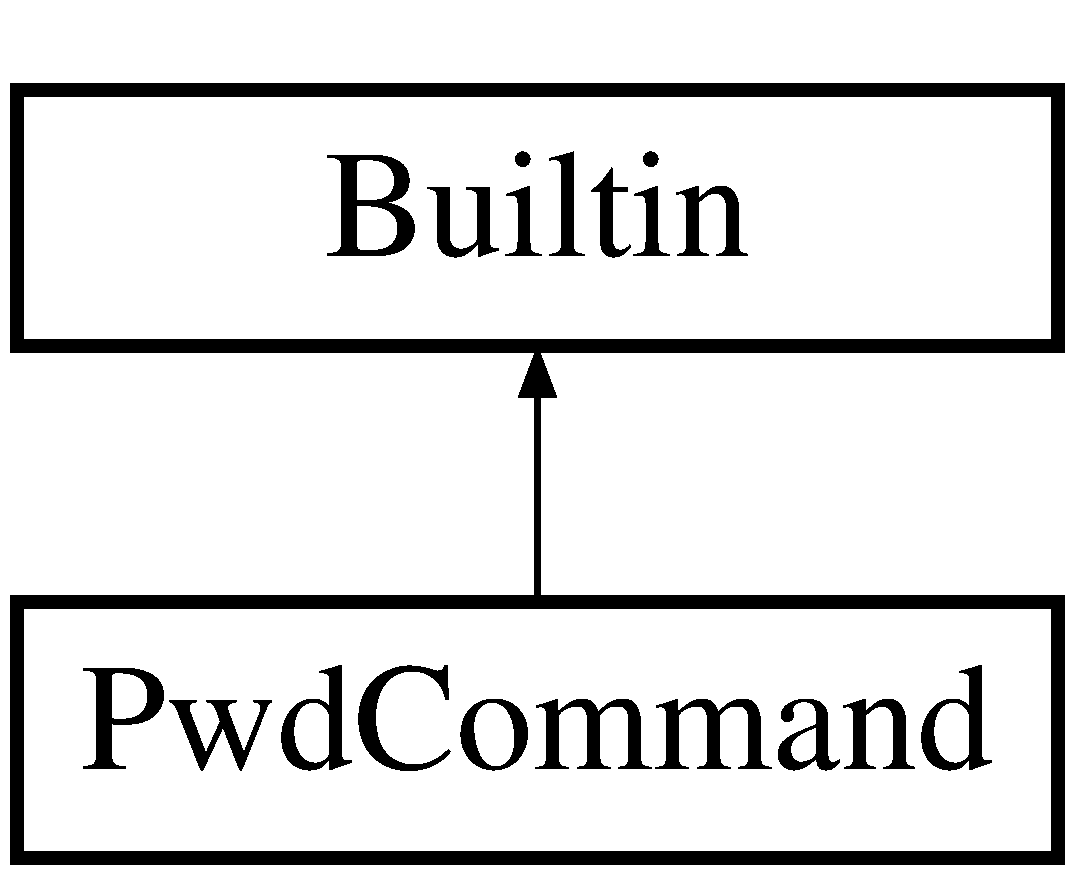
\includegraphics[height=2.000000cm]{classPwdCommand}
\end{center}
\end{figure}


\subsection{Detailed Description}
Classe que implementa o comando pwd. Sintaxe: pwd. 

The documentation for this class was generated from the following files:\begin{DoxyCompactItemize}
\item 
\hyperlink{Builtin_8hpp}{Builtin.hpp}\item 
\hyperlink{Builtin_8cpp}{Builtin.cpp}\end{DoxyCompactItemize}

\hypertarget{classgprof2dot_1_1SharkParser}{
\section{gprof2dot::SharkParser Class Reference}
\label{classgprof2dot_1_1SharkParser}\index{gprof2dot::SharkParser@{gprof2dot::SharkParser}}
}
Inheritance diagram for gprof2dot::SharkParser:\begin{figure}[H]
\begin{center}
\leavevmode
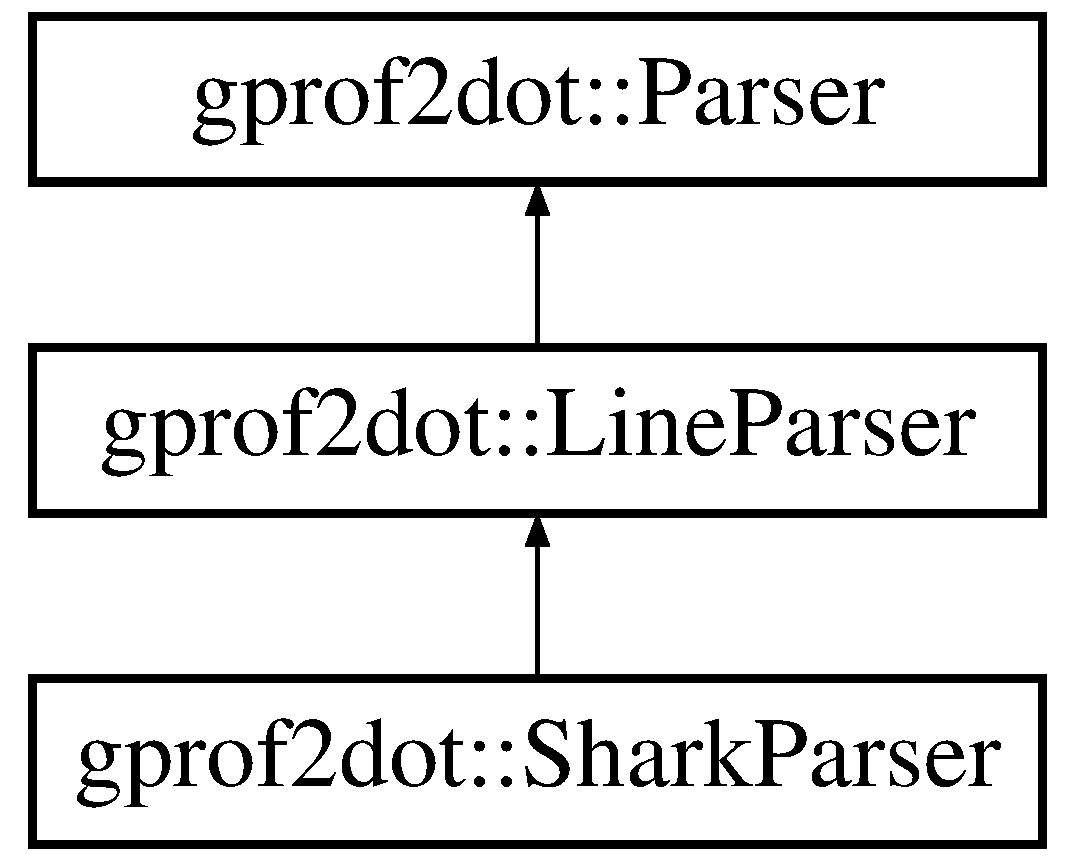
\includegraphics[height=3.000000cm]{classgprof2dot_1_1SharkParser}
\end{center}
\end{figure}
\subsection*{Public Member Functions}
\begin{DoxyCompactItemize}
\item 
def \hyperlink{classgprof2dot_1_1SharkParser_a763ed5b299f10d9a053462c99a074368}{\_\-\_\-init\_\-\_\-}
\item 
def \hyperlink{classgprof2dot_1_1SharkParser_a02ed27edea9d48d328db52b06d478991}{add\_\-entry}
\item 
def \hyperlink{classgprof2dot_1_1SharkParser_afc502a494e97444de1b0b79e4bbde1cb}{add\_\-callee}
\item 
def \hyperlink{classgprof2dot_1_1SharkParser_a50aedd037118d47393d3c8afe915be75}{parse}
\end{DoxyCompactItemize}
\subsection*{Public Attributes}
\begin{DoxyCompactItemize}
\item 
\hyperlink{classgprof2dot_1_1SharkParser_a3e10513646241304ce5208017eed21d4}{stack}
\item 
\hyperlink{classgprof2dot_1_1SharkParser_add53c92f98ac5751eba4bc9586fefb6c}{entries}
\end{DoxyCompactItemize}


\subsection{Detailed Description}
\begin{DoxyVerb}Parser for MacOSX Shark output.

Author: tom@dbservice.com
\end{DoxyVerb}
 

\subsection{Constructor \& Destructor Documentation}
\hypertarget{classgprof2dot_1_1SharkParser_a763ed5b299f10d9a053462c99a074368}{
\index{gprof2dot::SharkParser@{gprof2dot::SharkParser}!\_\-\_\-init\_\-\_\-@{\_\-\_\-init\_\-\_\-}}
\index{\_\-\_\-init\_\-\_\-@{\_\-\_\-init\_\-\_\-}!gprof2dot::SharkParser@{gprof2dot::SharkParser}}
\subsubsection[{\_\-\_\-init\_\-\_\-}]{\setlength{\rightskip}{0pt plus 5cm}def gprof2dot::SharkParser::\_\-\_\-init\_\-\_\- (
\begin{DoxyParamCaption}
\item[{}]{self, }
\item[{}]{infile}
\end{DoxyParamCaption}
)}}
\label{classgprof2dot_1_1SharkParser_a763ed5b299f10d9a053462c99a074368}


Reimplemented from \hyperlink{classgprof2dot_1_1LineParser_a9ab24f364f64a70181dd4156cea194c5}{gprof2dot::LineParser}.



\subsection{Member Function Documentation}
\hypertarget{classgprof2dot_1_1SharkParser_afc502a494e97444de1b0b79e4bbde1cb}{
\index{gprof2dot::SharkParser@{gprof2dot::SharkParser}!add\_\-callee@{add\_\-callee}}
\index{add\_\-callee@{add\_\-callee}!gprof2dot::SharkParser@{gprof2dot::SharkParser}}
\subsubsection[{add\_\-callee}]{\setlength{\rightskip}{0pt plus 5cm}def gprof2dot::SharkParser::add\_\-callee (
\begin{DoxyParamCaption}
\item[{}]{self, }
\item[{}]{function, }
\item[{}]{callee}
\end{DoxyParamCaption}
)}}
\label{classgprof2dot_1_1SharkParser_afc502a494e97444de1b0b79e4bbde1cb}
\hypertarget{classgprof2dot_1_1SharkParser_a02ed27edea9d48d328db52b06d478991}{
\index{gprof2dot::SharkParser@{gprof2dot::SharkParser}!add\_\-entry@{add\_\-entry}}
\index{add\_\-entry@{add\_\-entry}!gprof2dot::SharkParser@{gprof2dot::SharkParser}}
\subsubsection[{add\_\-entry}]{\setlength{\rightskip}{0pt plus 5cm}def gprof2dot::SharkParser::add\_\-entry (
\begin{DoxyParamCaption}
\item[{}]{self, }
\item[{}]{function}
\end{DoxyParamCaption}
)}}
\label{classgprof2dot_1_1SharkParser_a02ed27edea9d48d328db52b06d478991}
\hypertarget{classgprof2dot_1_1SharkParser_a50aedd037118d47393d3c8afe915be75}{
\index{gprof2dot::SharkParser@{gprof2dot::SharkParser}!parse@{parse}}
\index{parse@{parse}!gprof2dot::SharkParser@{gprof2dot::SharkParser}}
\subsubsection[{parse}]{\setlength{\rightskip}{0pt plus 5cm}def gprof2dot::SharkParser::parse (
\begin{DoxyParamCaption}
\item[{}]{self}
\end{DoxyParamCaption}
)}}
\label{classgprof2dot_1_1SharkParser_a50aedd037118d47393d3c8afe915be75}


Reimplemented from \hyperlink{classgprof2dot_1_1Parser_a681a0bc74e640c9c8e3d629dd03049fc}{gprof2dot::Parser}.



\subsection{Member Data Documentation}
\hypertarget{classgprof2dot_1_1SharkParser_add53c92f98ac5751eba4bc9586fefb6c}{
\index{gprof2dot::SharkParser@{gprof2dot::SharkParser}!entries@{entries}}
\index{entries@{entries}!gprof2dot::SharkParser@{gprof2dot::SharkParser}}
\subsubsection[{entries}]{\setlength{\rightskip}{0pt plus 5cm}{\bf gprof2dot::SharkParser::entries}}}
\label{classgprof2dot_1_1SharkParser_add53c92f98ac5751eba4bc9586fefb6c}
\hypertarget{classgprof2dot_1_1SharkParser_a3e10513646241304ce5208017eed21d4}{
\index{gprof2dot::SharkParser@{gprof2dot::SharkParser}!stack@{stack}}
\index{stack@{stack}!gprof2dot::SharkParser@{gprof2dot::SharkParser}}
\subsubsection[{stack}]{\setlength{\rightskip}{0pt plus 5cm}{\bf gprof2dot::SharkParser::stack}}}
\label{classgprof2dot_1_1SharkParser_a3e10513646241304ce5208017eed21d4}


The documentation for this class was generated from the following file:\begin{DoxyCompactItemize}
\item 
\hyperlink{gprof2dot_8py}{gprof2dot.py}\end{DoxyCompactItemize}

\hypertarget{classgprof2dot_1_1SleepyParser}{
\section{gprof2dot::SleepyParser Class Reference}
\label{classgprof2dot_1_1SleepyParser}\index{gprof2dot::SleepyParser@{gprof2dot::SleepyParser}}
}
Inheritance diagram for gprof2dot::SleepyParser:\begin{figure}[H]
\begin{center}
\leavevmode
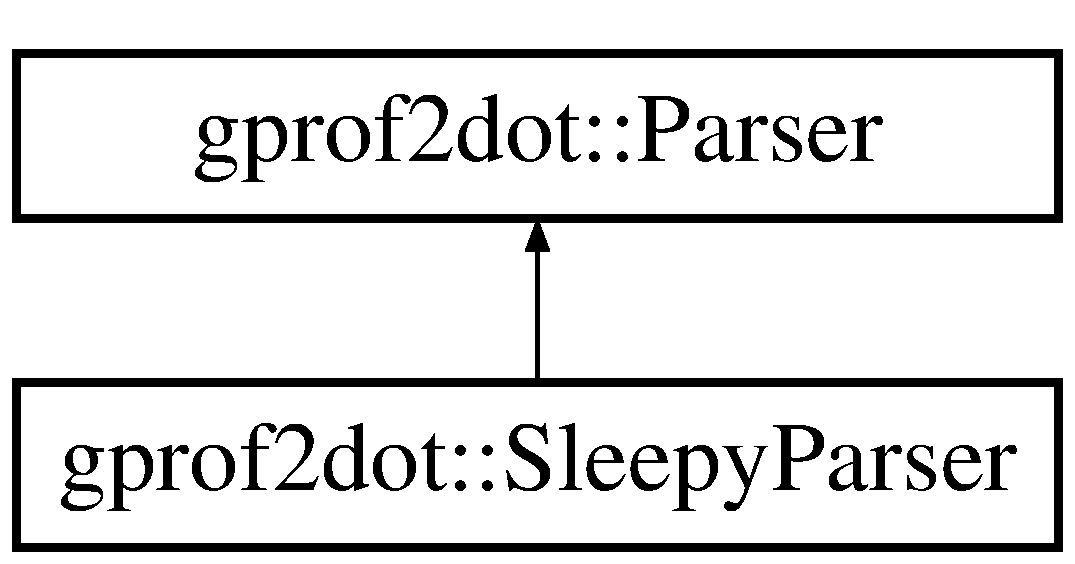
\includegraphics[height=2.000000cm]{classgprof2dot_1_1SleepyParser}
\end{center}
\end{figure}
\subsection*{Public Member Functions}
\begin{DoxyCompactItemize}
\item 
def \hyperlink{classgprof2dot_1_1SleepyParser_a8860ca8cc12c69c9b0646bb6fce19a48}{\_\-\_\-init\_\-\_\-}
\end{DoxyCompactItemize}
\subsection*{Public Attributes}
\begin{DoxyCompactItemize}
\item 
\hyperlink{classgprof2dot_1_1SleepyParser_aa4c6155496d6d6d966a97ac88bf37bbc}{database}
\item 
\hyperlink{classgprof2dot_1_1SleepyParser_a87af513951ab6c964913252846779c3c}{version\_\-0\_\-7}
\item 
\hyperlink{classgprof2dot_1_1SleepyParser_aa02364faa47a8b792bf2cfe6331b635d}{symbols}
\item 
\hyperlink{classgprof2dot_1_1SleepyParser_a3ea54178cb05f4bb06f138034d1a2ff3}{calls}
\item 
\hyperlink{classgprof2dot_1_1SleepyParser_a8b6a82e997115811f4d099fd494265ae}{profile}
\end{DoxyCompactItemize}


\subsection{Detailed Description}
\begin{DoxyVerb}Parser for GNU gprof output.

See also:
- http://www.codersnotes.com/sleepy/
- http://sleepygraph.sourceforge.net/
\end{DoxyVerb}
 

\subsection{Constructor \& Destructor Documentation}
\hypertarget{classgprof2dot_1_1SleepyParser_a8860ca8cc12c69c9b0646bb6fce19a48}{
\index{gprof2dot::SleepyParser@{gprof2dot::SleepyParser}!\_\-\_\-init\_\-\_\-@{\_\-\_\-init\_\-\_\-}}
\index{\_\-\_\-init\_\-\_\-@{\_\-\_\-init\_\-\_\-}!gprof2dot::SleepyParser@{gprof2dot::SleepyParser}}
\subsubsection[{\_\-\_\-init\_\-\_\-}]{\setlength{\rightskip}{0pt plus 5cm}def gprof2dot::SleepyParser::\_\-\_\-init\_\-\_\- (
\begin{DoxyParamCaption}
\item[{}]{self, }
\item[{}]{filename}
\end{DoxyParamCaption}
)}}
\label{classgprof2dot_1_1SleepyParser_a8860ca8cc12c69c9b0646bb6fce19a48}


\subsection{Member Data Documentation}
\hypertarget{classgprof2dot_1_1SleepyParser_a3ea54178cb05f4bb06f138034d1a2ff3}{
\index{gprof2dot::SleepyParser@{gprof2dot::SleepyParser}!calls@{calls}}
\index{calls@{calls}!gprof2dot::SleepyParser@{gprof2dot::SleepyParser}}
\subsubsection[{calls}]{\setlength{\rightskip}{0pt plus 5cm}{\bf gprof2dot::SleepyParser::calls}}}
\label{classgprof2dot_1_1SleepyParser_a3ea54178cb05f4bb06f138034d1a2ff3}
\hypertarget{classgprof2dot_1_1SleepyParser_aa4c6155496d6d6d966a97ac88bf37bbc}{
\index{gprof2dot::SleepyParser@{gprof2dot::SleepyParser}!database@{database}}
\index{database@{database}!gprof2dot::SleepyParser@{gprof2dot::SleepyParser}}
\subsubsection[{database}]{\setlength{\rightskip}{0pt plus 5cm}{\bf gprof2dot::SleepyParser::database}}}
\label{classgprof2dot_1_1SleepyParser_aa4c6155496d6d6d966a97ac88bf37bbc}
\hypertarget{classgprof2dot_1_1SleepyParser_a8b6a82e997115811f4d099fd494265ae}{
\index{gprof2dot::SleepyParser@{gprof2dot::SleepyParser}!profile@{profile}}
\index{profile@{profile}!gprof2dot::SleepyParser@{gprof2dot::SleepyParser}}
\subsubsection[{profile}]{\setlength{\rightskip}{0pt plus 5cm}{\bf gprof2dot::SleepyParser::profile}}}
\label{classgprof2dot_1_1SleepyParser_a8b6a82e997115811f4d099fd494265ae}
\hypertarget{classgprof2dot_1_1SleepyParser_aa02364faa47a8b792bf2cfe6331b635d}{
\index{gprof2dot::SleepyParser@{gprof2dot::SleepyParser}!symbols@{symbols}}
\index{symbols@{symbols}!gprof2dot::SleepyParser@{gprof2dot::SleepyParser}}
\subsubsection[{symbols}]{\setlength{\rightskip}{0pt plus 5cm}{\bf gprof2dot::SleepyParser::symbols}}}
\label{classgprof2dot_1_1SleepyParser_aa02364faa47a8b792bf2cfe6331b635d}
\hypertarget{classgprof2dot_1_1SleepyParser_a87af513951ab6c964913252846779c3c}{
\index{gprof2dot::SleepyParser@{gprof2dot::SleepyParser}!version\_\-0\_\-7@{version\_\-0\_\-7}}
\index{version\_\-0\_\-7@{version\_\-0\_\-7}!gprof2dot::SleepyParser@{gprof2dot::SleepyParser}}
\subsubsection[{version\_\-0\_\-7}]{\setlength{\rightskip}{0pt plus 5cm}{\bf gprof2dot::SleepyParser::version\_\-0\_\-7}}}
\label{classgprof2dot_1_1SleepyParser_a87af513951ab6c964913252846779c3c}


The documentation for this class was generated from the following file:\begin{DoxyCompactItemize}
\item 
\hyperlink{gprof2dot_8py}{gprof2dot.py}\end{DoxyCompactItemize}

\hypertarget{classgprof2dot_1_1Struct}{
\section{gprof2dot::Struct Class Reference}
\label{classgprof2dot_1_1Struct}\index{gprof2dot::Struct@{gprof2dot::Struct}}
}
\subsection*{Public Member Functions}
\begin{DoxyCompactItemize}
\item 
def \hyperlink{classgprof2dot_1_1Struct_a9564c586ef4474310d4577a75bfbe29c}{\_\-\_\-init\_\-\_\-}
\item 
def \hyperlink{classgprof2dot_1_1Struct_a6cac066ba246c533fed06a1bfa5ed3ff}{\_\-\_\-getattr\_\-\_\-}
\item 
def \hyperlink{classgprof2dot_1_1Struct_a2e057582d979c087a908a51a91d23e33}{\_\-\_\-setattr\_\-\_\-}
\item 
def \hyperlink{classgprof2dot_1_1Struct_afc0a4dd3f35b05e4ec8a02d96276cf81}{\_\-\_\-str\_\-\_\-}
\item 
def \hyperlink{classgprof2dot_1_1Struct_af62f737a65b392daec6c99d16d513fad}{\_\-\_\-repr\_\-\_\-}
\end{DoxyCompactItemize}


\subsection{Detailed Description}
\begin{DoxyVerb}Masquerade a dictionary with a structure-like behavior.\end{DoxyVerb}
 

\subsection{Constructor \& Destructor Documentation}
\hypertarget{classgprof2dot_1_1Struct_a9564c586ef4474310d4577a75bfbe29c}{
\index{gprof2dot::Struct@{gprof2dot::Struct}!\_\-\_\-init\_\-\_\-@{\_\-\_\-init\_\-\_\-}}
\index{\_\-\_\-init\_\-\_\-@{\_\-\_\-init\_\-\_\-}!gprof2dot::Struct@{gprof2dot::Struct}}
\subsubsection[{\_\-\_\-init\_\-\_\-}]{\setlength{\rightskip}{0pt plus 5cm}def gprof2dot::Struct::\_\-\_\-init\_\-\_\- (
\begin{DoxyParamCaption}
\item[{}]{self, }
\item[{}]{attrs = {\ttfamily None}}
\end{DoxyParamCaption}
)}}
\label{classgprof2dot_1_1Struct_a9564c586ef4474310d4577a75bfbe29c}


\subsection{Member Function Documentation}
\hypertarget{classgprof2dot_1_1Struct_a6cac066ba246c533fed06a1bfa5ed3ff}{
\index{gprof2dot::Struct@{gprof2dot::Struct}!\_\-\_\-getattr\_\-\_\-@{\_\-\_\-getattr\_\-\_\-}}
\index{\_\-\_\-getattr\_\-\_\-@{\_\-\_\-getattr\_\-\_\-}!gprof2dot::Struct@{gprof2dot::Struct}}
\subsubsection[{\_\-\_\-getattr\_\-\_\-}]{\setlength{\rightskip}{0pt plus 5cm}def gprof2dot::Struct::\_\-\_\-getattr\_\-\_\- (
\begin{DoxyParamCaption}
\item[{}]{self, }
\item[{}]{name}
\end{DoxyParamCaption}
)}}
\label{classgprof2dot_1_1Struct_a6cac066ba246c533fed06a1bfa5ed3ff}
\hypertarget{classgprof2dot_1_1Struct_af62f737a65b392daec6c99d16d513fad}{
\index{gprof2dot::Struct@{gprof2dot::Struct}!\_\-\_\-repr\_\-\_\-@{\_\-\_\-repr\_\-\_\-}}
\index{\_\-\_\-repr\_\-\_\-@{\_\-\_\-repr\_\-\_\-}!gprof2dot::Struct@{gprof2dot::Struct}}
\subsubsection[{\_\-\_\-repr\_\-\_\-}]{\setlength{\rightskip}{0pt plus 5cm}def gprof2dot::Struct::\_\-\_\-repr\_\-\_\- (
\begin{DoxyParamCaption}
\item[{}]{self}
\end{DoxyParamCaption}
)}}
\label{classgprof2dot_1_1Struct_af62f737a65b392daec6c99d16d513fad}
\hypertarget{classgprof2dot_1_1Struct_a2e057582d979c087a908a51a91d23e33}{
\index{gprof2dot::Struct@{gprof2dot::Struct}!\_\-\_\-setattr\_\-\_\-@{\_\-\_\-setattr\_\-\_\-}}
\index{\_\-\_\-setattr\_\-\_\-@{\_\-\_\-setattr\_\-\_\-}!gprof2dot::Struct@{gprof2dot::Struct}}
\subsubsection[{\_\-\_\-setattr\_\-\_\-}]{\setlength{\rightskip}{0pt plus 5cm}def gprof2dot::Struct::\_\-\_\-setattr\_\-\_\- (
\begin{DoxyParamCaption}
\item[{}]{self, }
\item[{}]{name, }
\item[{}]{value}
\end{DoxyParamCaption}
)}}
\label{classgprof2dot_1_1Struct_a2e057582d979c087a908a51a91d23e33}
\hypertarget{classgprof2dot_1_1Struct_afc0a4dd3f35b05e4ec8a02d96276cf81}{
\index{gprof2dot::Struct@{gprof2dot::Struct}!\_\-\_\-str\_\-\_\-@{\_\-\_\-str\_\-\_\-}}
\index{\_\-\_\-str\_\-\_\-@{\_\-\_\-str\_\-\_\-}!gprof2dot::Struct@{gprof2dot::Struct}}
\subsubsection[{\_\-\_\-str\_\-\_\-}]{\setlength{\rightskip}{0pt plus 5cm}def gprof2dot::Struct::\_\-\_\-str\_\-\_\- (
\begin{DoxyParamCaption}
\item[{}]{self}
\end{DoxyParamCaption}
)}}
\label{classgprof2dot_1_1Struct_afc0a4dd3f35b05e4ec8a02d96276cf81}


The documentation for this class was generated from the following file:\begin{DoxyCompactItemize}
\item 
\hyperlink{gprof2dot_8py}{gprof2dot.py}\end{DoxyCompactItemize}

\hypertarget{classgprof2dot_1_1SysprofParser}{
\section{gprof2dot::SysprofParser Class Reference}
\label{classgprof2dot_1_1SysprofParser}\index{gprof2dot::SysprofParser@{gprof2dot::SysprofParser}}
}
Inheritance diagram for gprof2dot::SysprofParser:\begin{figure}[H]
\begin{center}
\leavevmode
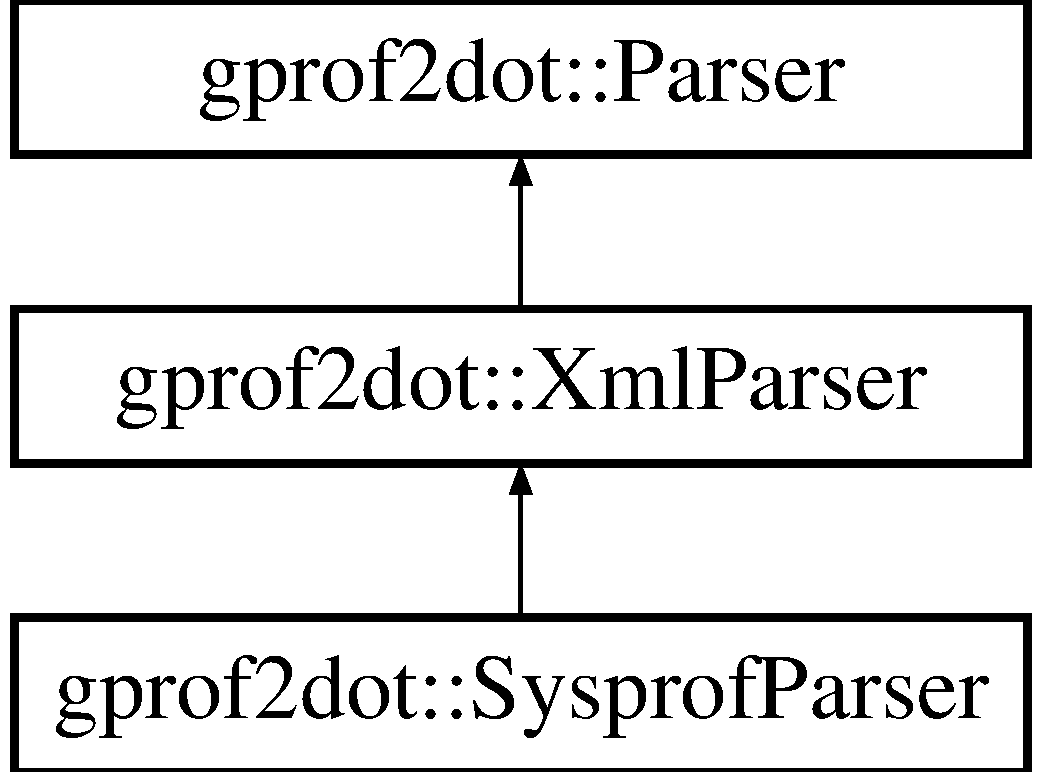
\includegraphics[height=3.000000cm]{classgprof2dot_1_1SysprofParser}
\end{center}
\end{figure}
\subsection*{Public Member Functions}
\begin{DoxyCompactItemize}
\item 
def \hyperlink{classgprof2dot_1_1SysprofParser_a17c27d48ae775d1e642aadaf28e07da9}{\_\-\_\-init\_\-\_\-}
\item 
def \hyperlink{classgprof2dot_1_1SysprofParser_acee5f7e208dd8f8d6ed73b88a70f2e7b}{parse}
\item 
def \hyperlink{classgprof2dot_1_1SysprofParser_a4829ef3c25ef3586b4fcc3bf89fc80ba}{parse\_\-items}
\item 
def \hyperlink{classgprof2dot_1_1SysprofParser_ad2c20a296b68975b702260c9dcc4d54a}{parse\_\-item}
\item 
def \hyperlink{classgprof2dot_1_1SysprofParser_abe14bb4484c34c33dfc1b3dd8c925b59}{parse\_\-values}
\item 
def \hyperlink{classgprof2dot_1_1SysprofParser_ae3375394224178726619d8f36a5f03b6}{parse\_\-value}
\item 
def \hyperlink{classgprof2dot_1_1SysprofParser_a21c26196a0c29b4478a22dd10b77c94b}{build\_\-profile}
\end{DoxyCompactItemize}


\subsection{Constructor \& Destructor Documentation}
\hypertarget{classgprof2dot_1_1SysprofParser_a17c27d48ae775d1e642aadaf28e07da9}{
\index{gprof2dot::SysprofParser@{gprof2dot::SysprofParser}!\_\-\_\-init\_\-\_\-@{\_\-\_\-init\_\-\_\-}}
\index{\_\-\_\-init\_\-\_\-@{\_\-\_\-init\_\-\_\-}!gprof2dot::SysprofParser@{gprof2dot::SysprofParser}}
\subsubsection[{\_\-\_\-init\_\-\_\-}]{\setlength{\rightskip}{0pt plus 5cm}def gprof2dot::SysprofParser::\_\-\_\-init\_\-\_\- (
\begin{DoxyParamCaption}
\item[{}]{self, }
\item[{}]{stream}
\end{DoxyParamCaption}
)}}
\label{classgprof2dot_1_1SysprofParser_a17c27d48ae775d1e642aadaf28e07da9}


Reimplemented from \hyperlink{classgprof2dot_1_1XmlParser_ac3307ca05e7e17b5b6a2b96e9782107e}{gprof2dot::XmlParser}.



\subsection{Member Function Documentation}
\hypertarget{classgprof2dot_1_1SysprofParser_a21c26196a0c29b4478a22dd10b77c94b}{
\index{gprof2dot::SysprofParser@{gprof2dot::SysprofParser}!build\_\-profile@{build\_\-profile}}
\index{build\_\-profile@{build\_\-profile}!gprof2dot::SysprofParser@{gprof2dot::SysprofParser}}
\subsubsection[{build\_\-profile}]{\setlength{\rightskip}{0pt plus 5cm}def gprof2dot::SysprofParser::build\_\-profile (
\begin{DoxyParamCaption}
\item[{}]{self, }
\item[{}]{objects, }
\item[{}]{nodes}
\end{DoxyParamCaption}
)}}
\label{classgprof2dot_1_1SysprofParser_a21c26196a0c29b4478a22dd10b77c94b}
\hypertarget{classgprof2dot_1_1SysprofParser_acee5f7e208dd8f8d6ed73b88a70f2e7b}{
\index{gprof2dot::SysprofParser@{gprof2dot::SysprofParser}!parse@{parse}}
\index{parse@{parse}!gprof2dot::SysprofParser@{gprof2dot::SysprofParser}}
\subsubsection[{parse}]{\setlength{\rightskip}{0pt plus 5cm}def gprof2dot::SysprofParser::parse (
\begin{DoxyParamCaption}
\item[{}]{self}
\end{DoxyParamCaption}
)}}
\label{classgprof2dot_1_1SysprofParser_acee5f7e208dd8f8d6ed73b88a70f2e7b}


Reimplemented from \hyperlink{classgprof2dot_1_1Parser_a681a0bc74e640c9c8e3d629dd03049fc}{gprof2dot::Parser}.

\hypertarget{classgprof2dot_1_1SysprofParser_ad2c20a296b68975b702260c9dcc4d54a}{
\index{gprof2dot::SysprofParser@{gprof2dot::SysprofParser}!parse\_\-item@{parse\_\-item}}
\index{parse\_\-item@{parse\_\-item}!gprof2dot::SysprofParser@{gprof2dot::SysprofParser}}
\subsubsection[{parse\_\-item}]{\setlength{\rightskip}{0pt plus 5cm}def gprof2dot::SysprofParser::parse\_\-item (
\begin{DoxyParamCaption}
\item[{}]{self, }
\item[{}]{name}
\end{DoxyParamCaption}
)}}
\label{classgprof2dot_1_1SysprofParser_ad2c20a296b68975b702260c9dcc4d54a}
\hypertarget{classgprof2dot_1_1SysprofParser_a4829ef3c25ef3586b4fcc3bf89fc80ba}{
\index{gprof2dot::SysprofParser@{gprof2dot::SysprofParser}!parse\_\-items@{parse\_\-items}}
\index{parse\_\-items@{parse\_\-items}!gprof2dot::SysprofParser@{gprof2dot::SysprofParser}}
\subsubsection[{parse\_\-items}]{\setlength{\rightskip}{0pt plus 5cm}def gprof2dot::SysprofParser::parse\_\-items (
\begin{DoxyParamCaption}
\item[{}]{self, }
\item[{}]{name}
\end{DoxyParamCaption}
)}}
\label{classgprof2dot_1_1SysprofParser_a4829ef3c25ef3586b4fcc3bf89fc80ba}
\hypertarget{classgprof2dot_1_1SysprofParser_ae3375394224178726619d8f36a5f03b6}{
\index{gprof2dot::SysprofParser@{gprof2dot::SysprofParser}!parse\_\-value@{parse\_\-value}}
\index{parse\_\-value@{parse\_\-value}!gprof2dot::SysprofParser@{gprof2dot::SysprofParser}}
\subsubsection[{parse\_\-value}]{\setlength{\rightskip}{0pt plus 5cm}def gprof2dot::SysprofParser::parse\_\-value (
\begin{DoxyParamCaption}
\item[{}]{self, }
\item[{}]{tag}
\end{DoxyParamCaption}
)}}
\label{classgprof2dot_1_1SysprofParser_ae3375394224178726619d8f36a5f03b6}
\hypertarget{classgprof2dot_1_1SysprofParser_abe14bb4484c34c33dfc1b3dd8c925b59}{
\index{gprof2dot::SysprofParser@{gprof2dot::SysprofParser}!parse\_\-values@{parse\_\-values}}
\index{parse\_\-values@{parse\_\-values}!gprof2dot::SysprofParser@{gprof2dot::SysprofParser}}
\subsubsection[{parse\_\-values}]{\setlength{\rightskip}{0pt plus 5cm}def gprof2dot::SysprofParser::parse\_\-values (
\begin{DoxyParamCaption}
\item[{}]{self}
\end{DoxyParamCaption}
)}}
\label{classgprof2dot_1_1SysprofParser_abe14bb4484c34c33dfc1b3dd8c925b59}


The documentation for this class was generated from the following file:\begin{DoxyCompactItemize}
\item 
\hyperlink{gprof2dot_8py}{gprof2dot.py}\end{DoxyCompactItemize}

\hypertarget{classgprof2dot_1_1Theme}{
\section{gprof2dot::Theme Class Reference}
\label{classgprof2dot_1_1Theme}\index{gprof2dot::Theme@{gprof2dot::Theme}}
}
\subsection*{Public Member Functions}
\begin{DoxyCompactItemize}
\item 
def \hyperlink{classgprof2dot_1_1Theme_a2276398a6eb51a85e845a9783f016de3}{\_\-\_\-init\_\-\_\-}
\item 
def \hyperlink{classgprof2dot_1_1Theme_a2aa94a61ff03ea9ecb2750a0bc973cc6}{graph\_\-bgcolor}
\item 
def \hyperlink{classgprof2dot_1_1Theme_ac19dbd4cd62fc32036f38281b4fb907d}{graph\_\-fontname}
\item 
def \hyperlink{classgprof2dot_1_1Theme_abdff38cc909ec02243380fe8c36d9ae3}{graph\_\-fontsize}
\item 
def \hyperlink{classgprof2dot_1_1Theme_af53963ae08324fb767cf33507939f2bb}{node\_\-bgcolor}
\item 
def \hyperlink{classgprof2dot_1_1Theme_a1da7ce754a3295e8d8b1c3ee894a26d9}{node\_\-fgcolor}
\item 
def \hyperlink{classgprof2dot_1_1Theme_a55ad08f330951306d25ce4136504ee99}{node\_\-fontsize}
\item 
def \hyperlink{classgprof2dot_1_1Theme_a85837bcc37f0f91e64f0ca2befee6b35}{edge\_\-color}
\item 
def \hyperlink{classgprof2dot_1_1Theme_ae4ab4caa326507a32a5ac37559233cef}{edge\_\-fontsize}
\item 
def \hyperlink{classgprof2dot_1_1Theme_a5189df543f27823cf5e63a34188ae4b7}{edge\_\-penwidth}
\item 
def \hyperlink{classgprof2dot_1_1Theme_a59ecac3b7ca9af819986f1a192bc09cf}{edge\_\-arrowsize}
\item 
def \hyperlink{classgprof2dot_1_1Theme_a1993203595812ae5d364c689ea8a702f}{fontsize}
\item 
def \hyperlink{classgprof2dot_1_1Theme_a7888f53604929f6c1589e0a687e9d3c7}{color}
\item 
def \hyperlink{classgprof2dot_1_1Theme_a43c94f70fd826ed62491db02de4ef46f}{hsl\_\-to\_\-rgb}
\end{DoxyCompactItemize}
\subsection*{Public Attributes}
\begin{DoxyCompactItemize}
\item 
\hyperlink{classgprof2dot_1_1Theme_a03ec2d6e3ef9d5bb373eb8902d0850c1}{bgcolor}
\item 
\hyperlink{classgprof2dot_1_1Theme_a00ec5eb4463c40669d90777fcb516754}{mincolor}
\item 
\hyperlink{classgprof2dot_1_1Theme_aac427429b605176076ef276b7c62adf3}{maxcolor}
\item 
\hyperlink{classgprof2dot_1_1Theme_a92dc7ef2582a13e357d1778eaafed468}{fontname}
\item 
\hyperlink{classgprof2dot_1_1Theme_a600f16c1724620261101751c2c2cb743}{minfontsize}
\item 
\hyperlink{classgprof2dot_1_1Theme_ac823da653b341ea9d3d6d7b10c70ae57}{maxfontsize}
\item 
\hyperlink{classgprof2dot_1_1Theme_a1c96fe1a046d8111c3217c84f95b1ebb}{minpenwidth}
\item 
\hyperlink{classgprof2dot_1_1Theme_a4815ce3e9f2a3c5f191304ee09b4047f}{maxpenwidth}
\item 
\hyperlink{classgprof2dot_1_1Theme_a835bb978ff2b2e23753c7bf775c7ee2b}{gamma}
\item 
\hyperlink{classgprof2dot_1_1Theme_a758b69f6b1ce9361ff7b387a2424c0e4}{skew}
\end{DoxyCompactItemize}


\subsection{Constructor \& Destructor Documentation}
\hypertarget{classgprof2dot_1_1Theme_a2276398a6eb51a85e845a9783f016de3}{
\index{gprof2dot::Theme@{gprof2dot::Theme}!\_\-\_\-init\_\-\_\-@{\_\-\_\-init\_\-\_\-}}
\index{\_\-\_\-init\_\-\_\-@{\_\-\_\-init\_\-\_\-}!gprof2dot::Theme@{gprof2dot::Theme}}
\subsubsection[{\_\-\_\-init\_\-\_\-}]{\setlength{\rightskip}{0pt plus 5cm}def gprof2dot::Theme::\_\-\_\-init\_\-\_\- (
\begin{DoxyParamCaption}
\item[{}]{self, }
\item[{}]{bgcolor = {\ttfamily (0.0,~0.0}, }
\item[{}]{mincolor = {\ttfamily (0.0,~0.0}, }
\item[{}]{maxcolor = {\ttfamily (0.0,~0.0}, }
\item[{}]{fontname = {\ttfamily \char`\"{}Arial\char`\"{}}, }
\item[{}]{minfontsize = {\ttfamily 10.0}, }
\item[{}]{maxfontsize = {\ttfamily 10.0}, }
\item[{}]{minpenwidth = {\ttfamily 0.5}, }
\item[{}]{maxpenwidth = {\ttfamily 4.0}, }
\item[{}]{gamma = {\ttfamily 2.2}, }
\item[{}]{skew = {\ttfamily 1.0}}
\end{DoxyParamCaption}
)}}
\label{classgprof2dot_1_1Theme_a2276398a6eb51a85e845a9783f016de3}


\subsection{Member Function Documentation}
\hypertarget{classgprof2dot_1_1Theme_a7888f53604929f6c1589e0a687e9d3c7}{
\index{gprof2dot::Theme@{gprof2dot::Theme}!color@{color}}
\index{color@{color}!gprof2dot::Theme@{gprof2dot::Theme}}
\subsubsection[{color}]{\setlength{\rightskip}{0pt plus 5cm}def gprof2dot::Theme::color (
\begin{DoxyParamCaption}
\item[{}]{self, }
\item[{}]{weight}
\end{DoxyParamCaption}
)}}
\label{classgprof2dot_1_1Theme_a7888f53604929f6c1589e0a687e9d3c7}
\hypertarget{classgprof2dot_1_1Theme_a59ecac3b7ca9af819986f1a192bc09cf}{
\index{gprof2dot::Theme@{gprof2dot::Theme}!edge\_\-arrowsize@{edge\_\-arrowsize}}
\index{edge\_\-arrowsize@{edge\_\-arrowsize}!gprof2dot::Theme@{gprof2dot::Theme}}
\subsubsection[{edge\_\-arrowsize}]{\setlength{\rightskip}{0pt plus 5cm}def gprof2dot::Theme::edge\_\-arrowsize (
\begin{DoxyParamCaption}
\item[{}]{self, }
\item[{}]{weight}
\end{DoxyParamCaption}
)}}
\label{classgprof2dot_1_1Theme_a59ecac3b7ca9af819986f1a192bc09cf}
\hypertarget{classgprof2dot_1_1Theme_a85837bcc37f0f91e64f0ca2befee6b35}{
\index{gprof2dot::Theme@{gprof2dot::Theme}!edge\_\-color@{edge\_\-color}}
\index{edge\_\-color@{edge\_\-color}!gprof2dot::Theme@{gprof2dot::Theme}}
\subsubsection[{edge\_\-color}]{\setlength{\rightskip}{0pt plus 5cm}def gprof2dot::Theme::edge\_\-color (
\begin{DoxyParamCaption}
\item[{}]{self, }
\item[{}]{weight}
\end{DoxyParamCaption}
)}}
\label{classgprof2dot_1_1Theme_a85837bcc37f0f91e64f0ca2befee6b35}
\hypertarget{classgprof2dot_1_1Theme_ae4ab4caa326507a32a5ac37559233cef}{
\index{gprof2dot::Theme@{gprof2dot::Theme}!edge\_\-fontsize@{edge\_\-fontsize}}
\index{edge\_\-fontsize@{edge\_\-fontsize}!gprof2dot::Theme@{gprof2dot::Theme}}
\subsubsection[{edge\_\-fontsize}]{\setlength{\rightskip}{0pt plus 5cm}def gprof2dot::Theme::edge\_\-fontsize (
\begin{DoxyParamCaption}
\item[{}]{self, }
\item[{}]{weight}
\end{DoxyParamCaption}
)}}
\label{classgprof2dot_1_1Theme_ae4ab4caa326507a32a5ac37559233cef}
\hypertarget{classgprof2dot_1_1Theme_a5189df543f27823cf5e63a34188ae4b7}{
\index{gprof2dot::Theme@{gprof2dot::Theme}!edge\_\-penwidth@{edge\_\-penwidth}}
\index{edge\_\-penwidth@{edge\_\-penwidth}!gprof2dot::Theme@{gprof2dot::Theme}}
\subsubsection[{edge\_\-penwidth}]{\setlength{\rightskip}{0pt plus 5cm}def gprof2dot::Theme::edge\_\-penwidth (
\begin{DoxyParamCaption}
\item[{}]{self, }
\item[{}]{weight}
\end{DoxyParamCaption}
)}}
\label{classgprof2dot_1_1Theme_a5189df543f27823cf5e63a34188ae4b7}
\hypertarget{classgprof2dot_1_1Theme_a1993203595812ae5d364c689ea8a702f}{
\index{gprof2dot::Theme@{gprof2dot::Theme}!fontsize@{fontsize}}
\index{fontsize@{fontsize}!gprof2dot::Theme@{gprof2dot::Theme}}
\subsubsection[{fontsize}]{\setlength{\rightskip}{0pt plus 5cm}def gprof2dot::Theme::fontsize (
\begin{DoxyParamCaption}
\item[{}]{self, }
\item[{}]{weight}
\end{DoxyParamCaption}
)}}
\label{classgprof2dot_1_1Theme_a1993203595812ae5d364c689ea8a702f}
\hypertarget{classgprof2dot_1_1Theme_a2aa94a61ff03ea9ecb2750a0bc973cc6}{
\index{gprof2dot::Theme@{gprof2dot::Theme}!graph\_\-bgcolor@{graph\_\-bgcolor}}
\index{graph\_\-bgcolor@{graph\_\-bgcolor}!gprof2dot::Theme@{gprof2dot::Theme}}
\subsubsection[{graph\_\-bgcolor}]{\setlength{\rightskip}{0pt plus 5cm}def gprof2dot::Theme::graph\_\-bgcolor (
\begin{DoxyParamCaption}
\item[{}]{self}
\end{DoxyParamCaption}
)}}
\label{classgprof2dot_1_1Theme_a2aa94a61ff03ea9ecb2750a0bc973cc6}
\hypertarget{classgprof2dot_1_1Theme_ac19dbd4cd62fc32036f38281b4fb907d}{
\index{gprof2dot::Theme@{gprof2dot::Theme}!graph\_\-fontname@{graph\_\-fontname}}
\index{graph\_\-fontname@{graph\_\-fontname}!gprof2dot::Theme@{gprof2dot::Theme}}
\subsubsection[{graph\_\-fontname}]{\setlength{\rightskip}{0pt plus 5cm}def gprof2dot::Theme::graph\_\-fontname (
\begin{DoxyParamCaption}
\item[{}]{self}
\end{DoxyParamCaption}
)}}
\label{classgprof2dot_1_1Theme_ac19dbd4cd62fc32036f38281b4fb907d}
\hypertarget{classgprof2dot_1_1Theme_abdff38cc909ec02243380fe8c36d9ae3}{
\index{gprof2dot::Theme@{gprof2dot::Theme}!graph\_\-fontsize@{graph\_\-fontsize}}
\index{graph\_\-fontsize@{graph\_\-fontsize}!gprof2dot::Theme@{gprof2dot::Theme}}
\subsubsection[{graph\_\-fontsize}]{\setlength{\rightskip}{0pt plus 5cm}def gprof2dot::Theme::graph\_\-fontsize (
\begin{DoxyParamCaption}
\item[{}]{self}
\end{DoxyParamCaption}
)}}
\label{classgprof2dot_1_1Theme_abdff38cc909ec02243380fe8c36d9ae3}
\hypertarget{classgprof2dot_1_1Theme_a43c94f70fd826ed62491db02de4ef46f}{
\index{gprof2dot::Theme@{gprof2dot::Theme}!hsl\_\-to\_\-rgb@{hsl\_\-to\_\-rgb}}
\index{hsl\_\-to\_\-rgb@{hsl\_\-to\_\-rgb}!gprof2dot::Theme@{gprof2dot::Theme}}
\subsubsection[{hsl\_\-to\_\-rgb}]{\setlength{\rightskip}{0pt plus 5cm}def gprof2dot::Theme::hsl\_\-to\_\-rgb (
\begin{DoxyParamCaption}
\item[{}]{self, }
\item[{}]{h, }
\item[{}]{s, }
\item[{}]{l}
\end{DoxyParamCaption}
)}}
\label{classgprof2dot_1_1Theme_a43c94f70fd826ed62491db02de4ef46f}
\begin{DoxyVerb}Convert a color from HSL color-model to RGB.

See also:
- http://www.w3.org/TR/css3-color/#hsl-color
\end{DoxyVerb}
 \hypertarget{classgprof2dot_1_1Theme_af53963ae08324fb767cf33507939f2bb}{
\index{gprof2dot::Theme@{gprof2dot::Theme}!node\_\-bgcolor@{node\_\-bgcolor}}
\index{node\_\-bgcolor@{node\_\-bgcolor}!gprof2dot::Theme@{gprof2dot::Theme}}
\subsubsection[{node\_\-bgcolor}]{\setlength{\rightskip}{0pt plus 5cm}def gprof2dot::Theme::node\_\-bgcolor (
\begin{DoxyParamCaption}
\item[{}]{self, }
\item[{}]{weight}
\end{DoxyParamCaption}
)}}
\label{classgprof2dot_1_1Theme_af53963ae08324fb767cf33507939f2bb}
\hypertarget{classgprof2dot_1_1Theme_a1da7ce754a3295e8d8b1c3ee894a26d9}{
\index{gprof2dot::Theme@{gprof2dot::Theme}!node\_\-fgcolor@{node\_\-fgcolor}}
\index{node\_\-fgcolor@{node\_\-fgcolor}!gprof2dot::Theme@{gprof2dot::Theme}}
\subsubsection[{node\_\-fgcolor}]{\setlength{\rightskip}{0pt plus 5cm}def gprof2dot::Theme::node\_\-fgcolor (
\begin{DoxyParamCaption}
\item[{}]{self, }
\item[{}]{weight}
\end{DoxyParamCaption}
)}}
\label{classgprof2dot_1_1Theme_a1da7ce754a3295e8d8b1c3ee894a26d9}
\hypertarget{classgprof2dot_1_1Theme_a55ad08f330951306d25ce4136504ee99}{
\index{gprof2dot::Theme@{gprof2dot::Theme}!node\_\-fontsize@{node\_\-fontsize}}
\index{node\_\-fontsize@{node\_\-fontsize}!gprof2dot::Theme@{gprof2dot::Theme}}
\subsubsection[{node\_\-fontsize}]{\setlength{\rightskip}{0pt plus 5cm}def gprof2dot::Theme::node\_\-fontsize (
\begin{DoxyParamCaption}
\item[{}]{self, }
\item[{}]{weight}
\end{DoxyParamCaption}
)}}
\label{classgprof2dot_1_1Theme_a55ad08f330951306d25ce4136504ee99}


\subsection{Member Data Documentation}
\hypertarget{classgprof2dot_1_1Theme_a03ec2d6e3ef9d5bb373eb8902d0850c1}{
\index{gprof2dot::Theme@{gprof2dot::Theme}!bgcolor@{bgcolor}}
\index{bgcolor@{bgcolor}!gprof2dot::Theme@{gprof2dot::Theme}}
\subsubsection[{bgcolor}]{\setlength{\rightskip}{0pt plus 5cm}{\bf gprof2dot::Theme::bgcolor}}}
\label{classgprof2dot_1_1Theme_a03ec2d6e3ef9d5bb373eb8902d0850c1}
\hypertarget{classgprof2dot_1_1Theme_a92dc7ef2582a13e357d1778eaafed468}{
\index{gprof2dot::Theme@{gprof2dot::Theme}!fontname@{fontname}}
\index{fontname@{fontname}!gprof2dot::Theme@{gprof2dot::Theme}}
\subsubsection[{fontname}]{\setlength{\rightskip}{0pt plus 5cm}{\bf gprof2dot::Theme::fontname}}}
\label{classgprof2dot_1_1Theme_a92dc7ef2582a13e357d1778eaafed468}
\hypertarget{classgprof2dot_1_1Theme_a835bb978ff2b2e23753c7bf775c7ee2b}{
\index{gprof2dot::Theme@{gprof2dot::Theme}!gamma@{gamma}}
\index{gamma@{gamma}!gprof2dot::Theme@{gprof2dot::Theme}}
\subsubsection[{gamma}]{\setlength{\rightskip}{0pt plus 5cm}{\bf gprof2dot::Theme::gamma}}}
\label{classgprof2dot_1_1Theme_a835bb978ff2b2e23753c7bf775c7ee2b}
\hypertarget{classgprof2dot_1_1Theme_aac427429b605176076ef276b7c62adf3}{
\index{gprof2dot::Theme@{gprof2dot::Theme}!maxcolor@{maxcolor}}
\index{maxcolor@{maxcolor}!gprof2dot::Theme@{gprof2dot::Theme}}
\subsubsection[{maxcolor}]{\setlength{\rightskip}{0pt plus 5cm}{\bf gprof2dot::Theme::maxcolor}}}
\label{classgprof2dot_1_1Theme_aac427429b605176076ef276b7c62adf3}
\hypertarget{classgprof2dot_1_1Theme_ac823da653b341ea9d3d6d7b10c70ae57}{
\index{gprof2dot::Theme@{gprof2dot::Theme}!maxfontsize@{maxfontsize}}
\index{maxfontsize@{maxfontsize}!gprof2dot::Theme@{gprof2dot::Theme}}
\subsubsection[{maxfontsize}]{\setlength{\rightskip}{0pt plus 5cm}{\bf gprof2dot::Theme::maxfontsize}}}
\label{classgprof2dot_1_1Theme_ac823da653b341ea9d3d6d7b10c70ae57}
\hypertarget{classgprof2dot_1_1Theme_a4815ce3e9f2a3c5f191304ee09b4047f}{
\index{gprof2dot::Theme@{gprof2dot::Theme}!maxpenwidth@{maxpenwidth}}
\index{maxpenwidth@{maxpenwidth}!gprof2dot::Theme@{gprof2dot::Theme}}
\subsubsection[{maxpenwidth}]{\setlength{\rightskip}{0pt plus 5cm}{\bf gprof2dot::Theme::maxpenwidth}}}
\label{classgprof2dot_1_1Theme_a4815ce3e9f2a3c5f191304ee09b4047f}
\hypertarget{classgprof2dot_1_1Theme_a00ec5eb4463c40669d90777fcb516754}{
\index{gprof2dot::Theme@{gprof2dot::Theme}!mincolor@{mincolor}}
\index{mincolor@{mincolor}!gprof2dot::Theme@{gprof2dot::Theme}}
\subsubsection[{mincolor}]{\setlength{\rightskip}{0pt plus 5cm}{\bf gprof2dot::Theme::mincolor}}}
\label{classgprof2dot_1_1Theme_a00ec5eb4463c40669d90777fcb516754}
\hypertarget{classgprof2dot_1_1Theme_a600f16c1724620261101751c2c2cb743}{
\index{gprof2dot::Theme@{gprof2dot::Theme}!minfontsize@{minfontsize}}
\index{minfontsize@{minfontsize}!gprof2dot::Theme@{gprof2dot::Theme}}
\subsubsection[{minfontsize}]{\setlength{\rightskip}{0pt plus 5cm}{\bf gprof2dot::Theme::minfontsize}}}
\label{classgprof2dot_1_1Theme_a600f16c1724620261101751c2c2cb743}
\hypertarget{classgprof2dot_1_1Theme_a1c96fe1a046d8111c3217c84f95b1ebb}{
\index{gprof2dot::Theme@{gprof2dot::Theme}!minpenwidth@{minpenwidth}}
\index{minpenwidth@{minpenwidth}!gprof2dot::Theme@{gprof2dot::Theme}}
\subsubsection[{minpenwidth}]{\setlength{\rightskip}{0pt plus 5cm}{\bf gprof2dot::Theme::minpenwidth}}}
\label{classgprof2dot_1_1Theme_a1c96fe1a046d8111c3217c84f95b1ebb}
\hypertarget{classgprof2dot_1_1Theme_a758b69f6b1ce9361ff7b387a2424c0e4}{
\index{gprof2dot::Theme@{gprof2dot::Theme}!skew@{skew}}
\index{skew@{skew}!gprof2dot::Theme@{gprof2dot::Theme}}
\subsubsection[{skew}]{\setlength{\rightskip}{0pt plus 5cm}{\bf gprof2dot::Theme::skew}}}
\label{classgprof2dot_1_1Theme_a758b69f6b1ce9361ff7b387a2424c0e4}


The documentation for this class was generated from the following file:\begin{DoxyCompactItemize}
\item 
\hyperlink{gprof2dot_8py}{gprof2dot.py}\end{DoxyCompactItemize}

\hypertarget{classgprof2dot_1_1UndefinedEvent}{
\section{gprof2dot::UndefinedEvent Class Reference}
\label{classgprof2dot_1_1UndefinedEvent}\index{gprof2dot::UndefinedEvent@{gprof2dot::UndefinedEvent}}
}
\subsection*{Public Member Functions}
\begin{DoxyCompactItemize}
\item 
def \hyperlink{classgprof2dot_1_1UndefinedEvent_a79c634e159403c839c56d657d93efa5f}{\_\-\_\-init\_\-\_\-}
\item 
def \hyperlink{classgprof2dot_1_1UndefinedEvent_aa49b08ed0b6f3c72670921e9c804f83a}{\_\-\_\-str\_\-\_\-}
\end{DoxyCompactItemize}
\subsection*{Public Attributes}
\begin{DoxyCompactItemize}
\item 
\hyperlink{classgprof2dot_1_1UndefinedEvent_a31dfa7826fc21fb3e0402d5f2f7dc673}{event}
\end{DoxyCompactItemize}


\subsection{Detailed Description}
\begin{DoxyVerb}Raised when attempting to get an event which is undefined.\end{DoxyVerb}
 

\subsection{Constructor \& Destructor Documentation}
\hypertarget{classgprof2dot_1_1UndefinedEvent_a79c634e159403c839c56d657d93efa5f}{
\index{gprof2dot::UndefinedEvent@{gprof2dot::UndefinedEvent}!\_\-\_\-init\_\-\_\-@{\_\-\_\-init\_\-\_\-}}
\index{\_\-\_\-init\_\-\_\-@{\_\-\_\-init\_\-\_\-}!gprof2dot::UndefinedEvent@{gprof2dot::UndefinedEvent}}
\subsubsection[{\_\-\_\-init\_\-\_\-}]{\setlength{\rightskip}{0pt plus 5cm}def gprof2dot::UndefinedEvent::\_\-\_\-init\_\-\_\- (
\begin{DoxyParamCaption}
\item[{}]{self, }
\item[{}]{event}
\end{DoxyParamCaption}
)}}
\label{classgprof2dot_1_1UndefinedEvent_a79c634e159403c839c56d657d93efa5f}


\subsection{Member Function Documentation}
\hypertarget{classgprof2dot_1_1UndefinedEvent_aa49b08ed0b6f3c72670921e9c804f83a}{
\index{gprof2dot::UndefinedEvent@{gprof2dot::UndefinedEvent}!\_\-\_\-str\_\-\_\-@{\_\-\_\-str\_\-\_\-}}
\index{\_\-\_\-str\_\-\_\-@{\_\-\_\-str\_\-\_\-}!gprof2dot::UndefinedEvent@{gprof2dot::UndefinedEvent}}
\subsubsection[{\_\-\_\-str\_\-\_\-}]{\setlength{\rightskip}{0pt plus 5cm}def gprof2dot::UndefinedEvent::\_\-\_\-str\_\-\_\- (
\begin{DoxyParamCaption}
\item[{}]{self}
\end{DoxyParamCaption}
)}}
\label{classgprof2dot_1_1UndefinedEvent_aa49b08ed0b6f3c72670921e9c804f83a}


\subsection{Member Data Documentation}
\hypertarget{classgprof2dot_1_1UndefinedEvent_a31dfa7826fc21fb3e0402d5f2f7dc673}{
\index{gprof2dot::UndefinedEvent@{gprof2dot::UndefinedEvent}!event@{event}}
\index{event@{event}!gprof2dot::UndefinedEvent@{gprof2dot::UndefinedEvent}}
\subsubsection[{event}]{\setlength{\rightskip}{0pt plus 5cm}{\bf gprof2dot::UndefinedEvent::event}}}
\label{classgprof2dot_1_1UndefinedEvent_a31dfa7826fc21fb3e0402d5f2f7dc673}


The documentation for this class was generated from the following file:\begin{DoxyCompactItemize}
\item 
\hyperlink{gprof2dot_8py}{gprof2dot.py}\end{DoxyCompactItemize}

\hypertarget{classgprof2dot_1_1XmlParser}{
\section{gprof2dot::XmlParser Class Reference}
\label{classgprof2dot_1_1XmlParser}\index{gprof2dot::XmlParser@{gprof2dot::XmlParser}}
}
Inheritance diagram for gprof2dot::XmlParser:\begin{figure}[H]
\begin{center}
\leavevmode
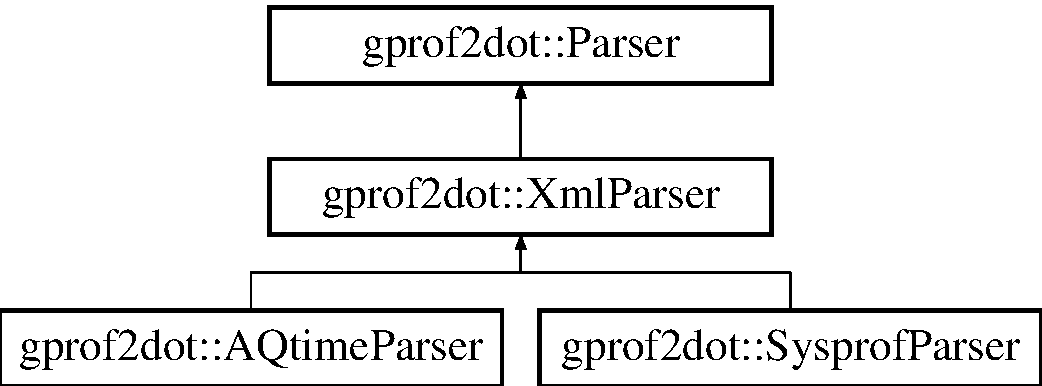
\includegraphics[height=3.000000cm]{classgprof2dot_1_1XmlParser}
\end{center}
\end{figure}
\subsection*{Public Member Functions}
\begin{DoxyCompactItemize}
\item 
def \hyperlink{classgprof2dot_1_1XmlParser_ac3307ca05e7e17b5b6a2b96e9782107e}{\_\-\_\-init\_\-\_\-}
\item 
def \hyperlink{classgprof2dot_1_1XmlParser_a3755f6ef42c3461d926ed78ec37ad1cb}{consume}
\item 
def \hyperlink{classgprof2dot_1_1XmlParser_a8f1de7b34709b190ee1fefa004be09f1}{match\_\-element\_\-start}
\item 
def \hyperlink{classgprof2dot_1_1XmlParser_a1f93debd5767a56ce359af7c0f9fb650}{match\_\-element\_\-end}
\item 
def \hyperlink{classgprof2dot_1_1XmlParser_a66b18e1ab93bd5a41e74a9eb9de17140}{element\_\-start}
\item 
def \hyperlink{classgprof2dot_1_1XmlParser_ac2a0a4aee58f3a4b302c005471f72b70}{element\_\-end}
\item 
def \hyperlink{classgprof2dot_1_1XmlParser_aba9557b2e5d26341f3696e789bf144fa}{character\_\-data}
\end{DoxyCompactItemize}
\subsection*{Public Attributes}
\begin{DoxyCompactItemize}
\item 
\hyperlink{classgprof2dot_1_1XmlParser_abb3dc2a67ab6387d51e7ba4eab7cf0e7}{tokenizer}
\item 
\hyperlink{classgprof2dot_1_1XmlParser_acf98651b1e43cc4bdc6804a79d0b35d5}{token}
\end{DoxyCompactItemize}


\subsection{Detailed Description}
\begin{DoxyVerb}Base XML document parser.\end{DoxyVerb}
 

\subsection{Constructor \& Destructor Documentation}
\hypertarget{classgprof2dot_1_1XmlParser_ac3307ca05e7e17b5b6a2b96e9782107e}{
\index{gprof2dot::XmlParser@{gprof2dot::XmlParser}!\_\-\_\-init\_\-\_\-@{\_\-\_\-init\_\-\_\-}}
\index{\_\-\_\-init\_\-\_\-@{\_\-\_\-init\_\-\_\-}!gprof2dot::XmlParser@{gprof2dot::XmlParser}}
\subsubsection[{\_\-\_\-init\_\-\_\-}]{\setlength{\rightskip}{0pt plus 5cm}def gprof2dot::XmlParser::\_\-\_\-init\_\-\_\- (
\begin{DoxyParamCaption}
\item[{}]{self, }
\item[{}]{fp}
\end{DoxyParamCaption}
)}}
\label{classgprof2dot_1_1XmlParser_ac3307ca05e7e17b5b6a2b96e9782107e}


Reimplemented in \hyperlink{classgprof2dot_1_1SysprofParser_a17c27d48ae775d1e642aadaf28e07da9}{gprof2dot::SysprofParser}, and \hyperlink{classgprof2dot_1_1AQtimeParser_aa59b49fada6b1c6fe520c4a54bca5e77}{gprof2dot::AQtimeParser}.



\subsection{Member Function Documentation}
\hypertarget{classgprof2dot_1_1XmlParser_aba9557b2e5d26341f3696e789bf144fa}{
\index{gprof2dot::XmlParser@{gprof2dot::XmlParser}!character\_\-data@{character\_\-data}}
\index{character\_\-data@{character\_\-data}!gprof2dot::XmlParser@{gprof2dot::XmlParser}}
\subsubsection[{character\_\-data}]{\setlength{\rightskip}{0pt plus 5cm}def gprof2dot::XmlParser::character\_\-data (
\begin{DoxyParamCaption}
\item[{}]{self, }
\item[{}]{strip = {\ttfamily True}}
\end{DoxyParamCaption}
)}}
\label{classgprof2dot_1_1XmlParser_aba9557b2e5d26341f3696e789bf144fa}
\hypertarget{classgprof2dot_1_1XmlParser_a3755f6ef42c3461d926ed78ec37ad1cb}{
\index{gprof2dot::XmlParser@{gprof2dot::XmlParser}!consume@{consume}}
\index{consume@{consume}!gprof2dot::XmlParser@{gprof2dot::XmlParser}}
\subsubsection[{consume}]{\setlength{\rightskip}{0pt plus 5cm}def gprof2dot::XmlParser::consume (
\begin{DoxyParamCaption}
\item[{}]{self}
\end{DoxyParamCaption}
)}}
\label{classgprof2dot_1_1XmlParser_a3755f6ef42c3461d926ed78ec37ad1cb}
\hypertarget{classgprof2dot_1_1XmlParser_ac2a0a4aee58f3a4b302c005471f72b70}{
\index{gprof2dot::XmlParser@{gprof2dot::XmlParser}!element\_\-end@{element\_\-end}}
\index{element\_\-end@{element\_\-end}!gprof2dot::XmlParser@{gprof2dot::XmlParser}}
\subsubsection[{element\_\-end}]{\setlength{\rightskip}{0pt plus 5cm}def gprof2dot::XmlParser::element\_\-end (
\begin{DoxyParamCaption}
\item[{}]{self, }
\item[{}]{name}
\end{DoxyParamCaption}
)}}
\label{classgprof2dot_1_1XmlParser_ac2a0a4aee58f3a4b302c005471f72b70}
\hypertarget{classgprof2dot_1_1XmlParser_a66b18e1ab93bd5a41e74a9eb9de17140}{
\index{gprof2dot::XmlParser@{gprof2dot::XmlParser}!element\_\-start@{element\_\-start}}
\index{element\_\-start@{element\_\-start}!gprof2dot::XmlParser@{gprof2dot::XmlParser}}
\subsubsection[{element\_\-start}]{\setlength{\rightskip}{0pt plus 5cm}def gprof2dot::XmlParser::element\_\-start (
\begin{DoxyParamCaption}
\item[{}]{self, }
\item[{}]{name}
\end{DoxyParamCaption}
)}}
\label{classgprof2dot_1_1XmlParser_a66b18e1ab93bd5a41e74a9eb9de17140}
\hypertarget{classgprof2dot_1_1XmlParser_a1f93debd5767a56ce359af7c0f9fb650}{
\index{gprof2dot::XmlParser@{gprof2dot::XmlParser}!match\_\-element\_\-end@{match\_\-element\_\-end}}
\index{match\_\-element\_\-end@{match\_\-element\_\-end}!gprof2dot::XmlParser@{gprof2dot::XmlParser}}
\subsubsection[{match\_\-element\_\-end}]{\setlength{\rightskip}{0pt plus 5cm}def gprof2dot::XmlParser::match\_\-element\_\-end (
\begin{DoxyParamCaption}
\item[{}]{self, }
\item[{}]{name}
\end{DoxyParamCaption}
)}}
\label{classgprof2dot_1_1XmlParser_a1f93debd5767a56ce359af7c0f9fb650}
\hypertarget{classgprof2dot_1_1XmlParser_a8f1de7b34709b190ee1fefa004be09f1}{
\index{gprof2dot::XmlParser@{gprof2dot::XmlParser}!match\_\-element\_\-start@{match\_\-element\_\-start}}
\index{match\_\-element\_\-start@{match\_\-element\_\-start}!gprof2dot::XmlParser@{gprof2dot::XmlParser}}
\subsubsection[{match\_\-element\_\-start}]{\setlength{\rightskip}{0pt plus 5cm}def gprof2dot::XmlParser::match\_\-element\_\-start (
\begin{DoxyParamCaption}
\item[{}]{self, }
\item[{}]{name}
\end{DoxyParamCaption}
)}}
\label{classgprof2dot_1_1XmlParser_a8f1de7b34709b190ee1fefa004be09f1}


\subsection{Member Data Documentation}
\hypertarget{classgprof2dot_1_1XmlParser_acf98651b1e43cc4bdc6804a79d0b35d5}{
\index{gprof2dot::XmlParser@{gprof2dot::XmlParser}!token@{token}}
\index{token@{token}!gprof2dot::XmlParser@{gprof2dot::XmlParser}}
\subsubsection[{token}]{\setlength{\rightskip}{0pt plus 5cm}{\bf gprof2dot::XmlParser::token}}}
\label{classgprof2dot_1_1XmlParser_acf98651b1e43cc4bdc6804a79d0b35d5}
\hypertarget{classgprof2dot_1_1XmlParser_abb3dc2a67ab6387d51e7ba4eab7cf0e7}{
\index{gprof2dot::XmlParser@{gprof2dot::XmlParser}!tokenizer@{tokenizer}}
\index{tokenizer@{tokenizer}!gprof2dot::XmlParser@{gprof2dot::XmlParser}}
\subsubsection[{tokenizer}]{\setlength{\rightskip}{0pt plus 5cm}{\bf gprof2dot::XmlParser::tokenizer}}}
\label{classgprof2dot_1_1XmlParser_abb3dc2a67ab6387d51e7ba4eab7cf0e7}


The documentation for this class was generated from the following file:\begin{DoxyCompactItemize}
\item 
\hyperlink{gprof2dot_8py}{gprof2dot.py}\end{DoxyCompactItemize}

\hypertarget{classgprof2dot_1_1XmlToken}{
\section{gprof2dot::XmlToken Class Reference}
\label{classgprof2dot_1_1XmlToken}\index{gprof2dot::XmlToken@{gprof2dot::XmlToken}}
}
\subsection*{Public Member Functions}
\begin{DoxyCompactItemize}
\item 
def \hyperlink{classgprof2dot_1_1XmlToken_a33d27d014983856e3c0bdad99d44f911}{\_\-\_\-init\_\-\_\-}
\item 
def \hyperlink{classgprof2dot_1_1XmlToken_ab6a72df66ff366c3213ad31bd0da1ff0}{\_\-\_\-str\_\-\_\-}
\end{DoxyCompactItemize}
\subsection*{Public Attributes}
\begin{DoxyCompactItemize}
\item 
\hyperlink{classgprof2dot_1_1XmlToken_a461559566df4c662376d5dd297a77d26}{type}
\item 
\hyperlink{classgprof2dot_1_1XmlToken_aedb0fd983c87a4a1be51fefce749c97c}{name\_\-or\_\-data}
\item 
\hyperlink{classgprof2dot_1_1XmlToken_aea87ce6e1d989ee97d7a2d89f47f3b5c}{attrs}
\item 
\hyperlink{classgprof2dot_1_1XmlToken_ad1f6dd4e80ff3e23a23d58fde94a9eaf}{line}
\item 
\hyperlink{classgprof2dot_1_1XmlToken_a6459b402cc6d278d498e6304232b06d6}{column}
\end{DoxyCompactItemize}


\subsection{Constructor \& Destructor Documentation}
\hypertarget{classgprof2dot_1_1XmlToken_a33d27d014983856e3c0bdad99d44f911}{
\index{gprof2dot::XmlToken@{gprof2dot::XmlToken}!\_\-\_\-init\_\-\_\-@{\_\-\_\-init\_\-\_\-}}
\index{\_\-\_\-init\_\-\_\-@{\_\-\_\-init\_\-\_\-}!gprof2dot::XmlToken@{gprof2dot::XmlToken}}
\subsubsection[{\_\-\_\-init\_\-\_\-}]{\setlength{\rightskip}{0pt plus 5cm}def gprof2dot::XmlToken::\_\-\_\-init\_\-\_\- (
\begin{DoxyParamCaption}
\item[{}]{self, }
\item[{}]{type, }
\item[{}]{name\_\-or\_\-data, }
\item[{}]{attrs = {\ttfamily None}, }
\item[{}]{line = {\ttfamily None}, }
\item[{}]{column = {\ttfamily None}}
\end{DoxyParamCaption}
)}}
\label{classgprof2dot_1_1XmlToken_a33d27d014983856e3c0bdad99d44f911}


\subsection{Member Function Documentation}
\hypertarget{classgprof2dot_1_1XmlToken_ab6a72df66ff366c3213ad31bd0da1ff0}{
\index{gprof2dot::XmlToken@{gprof2dot::XmlToken}!\_\-\_\-str\_\-\_\-@{\_\-\_\-str\_\-\_\-}}
\index{\_\-\_\-str\_\-\_\-@{\_\-\_\-str\_\-\_\-}!gprof2dot::XmlToken@{gprof2dot::XmlToken}}
\subsubsection[{\_\-\_\-str\_\-\_\-}]{\setlength{\rightskip}{0pt plus 5cm}def gprof2dot::XmlToken::\_\-\_\-str\_\-\_\- (
\begin{DoxyParamCaption}
\item[{}]{self}
\end{DoxyParamCaption}
)}}
\label{classgprof2dot_1_1XmlToken_ab6a72df66ff366c3213ad31bd0da1ff0}


\subsection{Member Data Documentation}
\hypertarget{classgprof2dot_1_1XmlToken_aea87ce6e1d989ee97d7a2d89f47f3b5c}{
\index{gprof2dot::XmlToken@{gprof2dot::XmlToken}!attrs@{attrs}}
\index{attrs@{attrs}!gprof2dot::XmlToken@{gprof2dot::XmlToken}}
\subsubsection[{attrs}]{\setlength{\rightskip}{0pt plus 5cm}{\bf gprof2dot::XmlToken::attrs}}}
\label{classgprof2dot_1_1XmlToken_aea87ce6e1d989ee97d7a2d89f47f3b5c}
\hypertarget{classgprof2dot_1_1XmlToken_a6459b402cc6d278d498e6304232b06d6}{
\index{gprof2dot::XmlToken@{gprof2dot::XmlToken}!column@{column}}
\index{column@{column}!gprof2dot::XmlToken@{gprof2dot::XmlToken}}
\subsubsection[{column}]{\setlength{\rightskip}{0pt plus 5cm}{\bf gprof2dot::XmlToken::column}}}
\label{classgprof2dot_1_1XmlToken_a6459b402cc6d278d498e6304232b06d6}
\hypertarget{classgprof2dot_1_1XmlToken_ad1f6dd4e80ff3e23a23d58fde94a9eaf}{
\index{gprof2dot::XmlToken@{gprof2dot::XmlToken}!line@{line}}
\index{line@{line}!gprof2dot::XmlToken@{gprof2dot::XmlToken}}
\subsubsection[{line}]{\setlength{\rightskip}{0pt plus 5cm}{\bf gprof2dot::XmlToken::line}}}
\label{classgprof2dot_1_1XmlToken_ad1f6dd4e80ff3e23a23d58fde94a9eaf}
\hypertarget{classgprof2dot_1_1XmlToken_aedb0fd983c87a4a1be51fefce749c97c}{
\index{gprof2dot::XmlToken@{gprof2dot::XmlToken}!name\_\-or\_\-data@{name\_\-or\_\-data}}
\index{name\_\-or\_\-data@{name\_\-or\_\-data}!gprof2dot::XmlToken@{gprof2dot::XmlToken}}
\subsubsection[{name\_\-or\_\-data}]{\setlength{\rightskip}{0pt plus 5cm}{\bf gprof2dot::XmlToken::name\_\-or\_\-data}}}
\label{classgprof2dot_1_1XmlToken_aedb0fd983c87a4a1be51fefce749c97c}
\hypertarget{classgprof2dot_1_1XmlToken_a461559566df4c662376d5dd297a77d26}{
\index{gprof2dot::XmlToken@{gprof2dot::XmlToken}!type@{type}}
\index{type@{type}!gprof2dot::XmlToken@{gprof2dot::XmlToken}}
\subsubsection[{type}]{\setlength{\rightskip}{0pt plus 5cm}{\bf gprof2dot::XmlToken::type}}}
\label{classgprof2dot_1_1XmlToken_a461559566df4c662376d5dd297a77d26}


The documentation for this class was generated from the following file:\begin{DoxyCompactItemize}
\item 
\hyperlink{gprof2dot_8py}{gprof2dot.py}\end{DoxyCompactItemize}

\hypertarget{classgprof2dot_1_1XmlTokenizer}{
\section{gprof2dot::XmlTokenizer Class Reference}
\label{classgprof2dot_1_1XmlTokenizer}\index{gprof2dot::XmlTokenizer@{gprof2dot::XmlTokenizer}}
}
\subsection*{Public Member Functions}
\begin{DoxyCompactItemize}
\item 
def \hyperlink{classgprof2dot_1_1XmlTokenizer_ae1f45ca5dbb6c4dce21534be2aa3643f}{\_\-\_\-init\_\-\_\-}
\item 
def \hyperlink{classgprof2dot_1_1XmlTokenizer_a80681c721f8cca08d474fc1ebba45f2e}{handle\_\-element\_\-start}
\item 
def \hyperlink{classgprof2dot_1_1XmlTokenizer_a18370d070bda2a5d795818fcacc67b9b}{handle\_\-element\_\-end}
\item 
def \hyperlink{classgprof2dot_1_1XmlTokenizer_a18c5bde4d75a54eee88467c0ce575318}{handle\_\-character\_\-data}
\item 
def \hyperlink{classgprof2dot_1_1XmlTokenizer_aee80d31081b69f03bbd7f6570e95553c}{finish\_\-character\_\-data}
\item 
def \hyperlink{classgprof2dot_1_1XmlTokenizer_a77ec97f2e711ca509c3b15d5c8f8deb0}{next}
\item 
def \hyperlink{classgprof2dot_1_1XmlTokenizer_ac2aacdda25050b6d645e97c2a511739b}{pos}
\end{DoxyCompactItemize}
\subsection*{Public Attributes}
\begin{DoxyCompactItemize}
\item 
\hyperlink{classgprof2dot_1_1XmlTokenizer_adcf837640c298212adaaf3fa97967ad7}{fp}
\item 
\hyperlink{classgprof2dot_1_1XmlTokenizer_a463b3e42d9b9d9cf1135d61a302123e5}{tokens}
\item 
\hyperlink{classgprof2dot_1_1XmlTokenizer_acf89c22a97b9ecfd1985ece5c88f4626}{index}
\item 
\hyperlink{classgprof2dot_1_1XmlTokenizer_a2fcb60f0f699e70e34ce340569d15476}{final}
\item 
\hyperlink{classgprof2dot_1_1XmlTokenizer_acf3445af8c53403394b50b0e75f09948}{skip\_\-ws}
\item 
\hyperlink{classgprof2dot_1_1XmlTokenizer_a04573673dad3be8574a7ad8d35166a19}{character\_\-pos}
\item 
\hyperlink{classgprof2dot_1_1XmlTokenizer_a84df3599b0cf4ebdae88952b1badea56}{character\_\-data}
\item 
\hyperlink{classgprof2dot_1_1XmlTokenizer_a98db4e33433d6d6970c8df9cfde92c9f}{parser}
\end{DoxyCompactItemize}


\subsection{Detailed Description}
\begin{DoxyVerb}Expat based XML tokenizer.\end{DoxyVerb}
 

\subsection{Constructor \& Destructor Documentation}
\hypertarget{classgprof2dot_1_1XmlTokenizer_ae1f45ca5dbb6c4dce21534be2aa3643f}{
\index{gprof2dot::XmlTokenizer@{gprof2dot::XmlTokenizer}!\_\-\_\-init\_\-\_\-@{\_\-\_\-init\_\-\_\-}}
\index{\_\-\_\-init\_\-\_\-@{\_\-\_\-init\_\-\_\-}!gprof2dot::XmlTokenizer@{gprof2dot::XmlTokenizer}}
\subsubsection[{\_\-\_\-init\_\-\_\-}]{\setlength{\rightskip}{0pt plus 5cm}def gprof2dot::XmlTokenizer::\_\-\_\-init\_\-\_\- (
\begin{DoxyParamCaption}
\item[{}]{self, }
\item[{}]{fp, }
\item[{}]{skip\_\-ws = {\ttfamily True}}
\end{DoxyParamCaption}
)}}
\label{classgprof2dot_1_1XmlTokenizer_ae1f45ca5dbb6c4dce21534be2aa3643f}


\subsection{Member Function Documentation}
\hypertarget{classgprof2dot_1_1XmlTokenizer_aee80d31081b69f03bbd7f6570e95553c}{
\index{gprof2dot::XmlTokenizer@{gprof2dot::XmlTokenizer}!finish\_\-character\_\-data@{finish\_\-character\_\-data}}
\index{finish\_\-character\_\-data@{finish\_\-character\_\-data}!gprof2dot::XmlTokenizer@{gprof2dot::XmlTokenizer}}
\subsubsection[{finish\_\-character\_\-data}]{\setlength{\rightskip}{0pt plus 5cm}def gprof2dot::XmlTokenizer::finish\_\-character\_\-data (
\begin{DoxyParamCaption}
\item[{}]{self}
\end{DoxyParamCaption}
)}}
\label{classgprof2dot_1_1XmlTokenizer_aee80d31081b69f03bbd7f6570e95553c}
\hypertarget{classgprof2dot_1_1XmlTokenizer_a18c5bde4d75a54eee88467c0ce575318}{
\index{gprof2dot::XmlTokenizer@{gprof2dot::XmlTokenizer}!handle\_\-character\_\-data@{handle\_\-character\_\-data}}
\index{handle\_\-character\_\-data@{handle\_\-character\_\-data}!gprof2dot::XmlTokenizer@{gprof2dot::XmlTokenizer}}
\subsubsection[{handle\_\-character\_\-data}]{\setlength{\rightskip}{0pt plus 5cm}def gprof2dot::XmlTokenizer::handle\_\-character\_\-data (
\begin{DoxyParamCaption}
\item[{}]{self, }
\item[{}]{data}
\end{DoxyParamCaption}
)}}
\label{classgprof2dot_1_1XmlTokenizer_a18c5bde4d75a54eee88467c0ce575318}
\hypertarget{classgprof2dot_1_1XmlTokenizer_a18370d070bda2a5d795818fcacc67b9b}{
\index{gprof2dot::XmlTokenizer@{gprof2dot::XmlTokenizer}!handle\_\-element\_\-end@{handle\_\-element\_\-end}}
\index{handle\_\-element\_\-end@{handle\_\-element\_\-end}!gprof2dot::XmlTokenizer@{gprof2dot::XmlTokenizer}}
\subsubsection[{handle\_\-element\_\-end}]{\setlength{\rightskip}{0pt plus 5cm}def gprof2dot::XmlTokenizer::handle\_\-element\_\-end (
\begin{DoxyParamCaption}
\item[{}]{self, }
\item[{}]{name}
\end{DoxyParamCaption}
)}}
\label{classgprof2dot_1_1XmlTokenizer_a18370d070bda2a5d795818fcacc67b9b}
\hypertarget{classgprof2dot_1_1XmlTokenizer_a80681c721f8cca08d474fc1ebba45f2e}{
\index{gprof2dot::XmlTokenizer@{gprof2dot::XmlTokenizer}!handle\_\-element\_\-start@{handle\_\-element\_\-start}}
\index{handle\_\-element\_\-start@{handle\_\-element\_\-start}!gprof2dot::XmlTokenizer@{gprof2dot::XmlTokenizer}}
\subsubsection[{handle\_\-element\_\-start}]{\setlength{\rightskip}{0pt plus 5cm}def gprof2dot::XmlTokenizer::handle\_\-element\_\-start (
\begin{DoxyParamCaption}
\item[{}]{self, }
\item[{}]{name, }
\item[{}]{attributes}
\end{DoxyParamCaption}
)}}
\label{classgprof2dot_1_1XmlTokenizer_a80681c721f8cca08d474fc1ebba45f2e}
\hypertarget{classgprof2dot_1_1XmlTokenizer_a77ec97f2e711ca509c3b15d5c8f8deb0}{
\index{gprof2dot::XmlTokenizer@{gprof2dot::XmlTokenizer}!next@{next}}
\index{next@{next}!gprof2dot::XmlTokenizer@{gprof2dot::XmlTokenizer}}
\subsubsection[{next}]{\setlength{\rightskip}{0pt plus 5cm}def gprof2dot::XmlTokenizer::next (
\begin{DoxyParamCaption}
\item[{}]{self}
\end{DoxyParamCaption}
)}}
\label{classgprof2dot_1_1XmlTokenizer_a77ec97f2e711ca509c3b15d5c8f8deb0}
\hypertarget{classgprof2dot_1_1XmlTokenizer_ac2aacdda25050b6d645e97c2a511739b}{
\index{gprof2dot::XmlTokenizer@{gprof2dot::XmlTokenizer}!pos@{pos}}
\index{pos@{pos}!gprof2dot::XmlTokenizer@{gprof2dot::XmlTokenizer}}
\subsubsection[{pos}]{\setlength{\rightskip}{0pt plus 5cm}def gprof2dot::XmlTokenizer::pos (
\begin{DoxyParamCaption}
\item[{}]{self}
\end{DoxyParamCaption}
)}}
\label{classgprof2dot_1_1XmlTokenizer_ac2aacdda25050b6d645e97c2a511739b}


\subsection{Member Data Documentation}
\hypertarget{classgprof2dot_1_1XmlTokenizer_a84df3599b0cf4ebdae88952b1badea56}{
\index{gprof2dot::XmlTokenizer@{gprof2dot::XmlTokenizer}!character\_\-data@{character\_\-data}}
\index{character\_\-data@{character\_\-data}!gprof2dot::XmlTokenizer@{gprof2dot::XmlTokenizer}}
\subsubsection[{character\_\-data}]{\setlength{\rightskip}{0pt plus 5cm}{\bf gprof2dot::XmlTokenizer::character\_\-data}}}
\label{classgprof2dot_1_1XmlTokenizer_a84df3599b0cf4ebdae88952b1badea56}
\hypertarget{classgprof2dot_1_1XmlTokenizer_a04573673dad3be8574a7ad8d35166a19}{
\index{gprof2dot::XmlTokenizer@{gprof2dot::XmlTokenizer}!character\_\-pos@{character\_\-pos}}
\index{character\_\-pos@{character\_\-pos}!gprof2dot::XmlTokenizer@{gprof2dot::XmlTokenizer}}
\subsubsection[{character\_\-pos}]{\setlength{\rightskip}{0pt plus 5cm}{\bf gprof2dot::XmlTokenizer::character\_\-pos}}}
\label{classgprof2dot_1_1XmlTokenizer_a04573673dad3be8574a7ad8d35166a19}
\hypertarget{classgprof2dot_1_1XmlTokenizer_a2fcb60f0f699e70e34ce340569d15476}{
\index{gprof2dot::XmlTokenizer@{gprof2dot::XmlTokenizer}!final@{final}}
\index{final@{final}!gprof2dot::XmlTokenizer@{gprof2dot::XmlTokenizer}}
\subsubsection[{final}]{\setlength{\rightskip}{0pt plus 5cm}{\bf gprof2dot::XmlTokenizer::final}}}
\label{classgprof2dot_1_1XmlTokenizer_a2fcb60f0f699e70e34ce340569d15476}
\hypertarget{classgprof2dot_1_1XmlTokenizer_adcf837640c298212adaaf3fa97967ad7}{
\index{gprof2dot::XmlTokenizer@{gprof2dot::XmlTokenizer}!fp@{fp}}
\index{fp@{fp}!gprof2dot::XmlTokenizer@{gprof2dot::XmlTokenizer}}
\subsubsection[{fp}]{\setlength{\rightskip}{0pt plus 5cm}{\bf gprof2dot::XmlTokenizer::fp}}}
\label{classgprof2dot_1_1XmlTokenizer_adcf837640c298212adaaf3fa97967ad7}
\hypertarget{classgprof2dot_1_1XmlTokenizer_acf89c22a97b9ecfd1985ece5c88f4626}{
\index{gprof2dot::XmlTokenizer@{gprof2dot::XmlTokenizer}!index@{index}}
\index{index@{index}!gprof2dot::XmlTokenizer@{gprof2dot::XmlTokenizer}}
\subsubsection[{index}]{\setlength{\rightskip}{0pt plus 5cm}{\bf gprof2dot::XmlTokenizer::index}}}
\label{classgprof2dot_1_1XmlTokenizer_acf89c22a97b9ecfd1985ece5c88f4626}
\hypertarget{classgprof2dot_1_1XmlTokenizer_a98db4e33433d6d6970c8df9cfde92c9f}{
\index{gprof2dot::XmlTokenizer@{gprof2dot::XmlTokenizer}!parser@{parser}}
\index{parser@{parser}!gprof2dot::XmlTokenizer@{gprof2dot::XmlTokenizer}}
\subsubsection[{parser}]{\setlength{\rightskip}{0pt plus 5cm}{\bf gprof2dot::XmlTokenizer::parser}}}
\label{classgprof2dot_1_1XmlTokenizer_a98db4e33433d6d6970c8df9cfde92c9f}
\hypertarget{classgprof2dot_1_1XmlTokenizer_acf3445af8c53403394b50b0e75f09948}{
\index{gprof2dot::XmlTokenizer@{gprof2dot::XmlTokenizer}!skip\_\-ws@{skip\_\-ws}}
\index{skip\_\-ws@{skip\_\-ws}!gprof2dot::XmlTokenizer@{gprof2dot::XmlTokenizer}}
\subsubsection[{skip\_\-ws}]{\setlength{\rightskip}{0pt plus 5cm}{\bf gprof2dot::XmlTokenizer::skip\_\-ws}}}
\label{classgprof2dot_1_1XmlTokenizer_acf3445af8c53403394b50b0e75f09948}
\hypertarget{classgprof2dot_1_1XmlTokenizer_a463b3e42d9b9d9cf1135d61a302123e5}{
\index{gprof2dot::XmlTokenizer@{gprof2dot::XmlTokenizer}!tokens@{tokens}}
\index{tokens@{tokens}!gprof2dot::XmlTokenizer@{gprof2dot::XmlTokenizer}}
\subsubsection[{tokens}]{\setlength{\rightskip}{0pt plus 5cm}{\bf gprof2dot::XmlTokenizer::tokens}}}
\label{classgprof2dot_1_1XmlTokenizer_a463b3e42d9b9d9cf1135d61a302123e5}


The documentation for this class was generated from the following file:\begin{DoxyCompactItemize}
\item 
\hyperlink{gprof2dot_8py}{gprof2dot.py}\end{DoxyCompactItemize}

\hypertarget{classgprof2dot_1_1XmlTokenMismatch}{
\section{gprof2dot::XmlTokenMismatch Class Reference}
\label{classgprof2dot_1_1XmlTokenMismatch}\index{gprof2dot::XmlTokenMismatch@{gprof2dot::XmlTokenMismatch}}
}
\subsection*{Public Member Functions}
\begin{DoxyCompactItemize}
\item 
def \hyperlink{classgprof2dot_1_1XmlTokenMismatch_a5f305439f12a07ede6c3993fdef91af2}{\_\-\_\-init\_\-\_\-}
\item 
def \hyperlink{classgprof2dot_1_1XmlTokenMismatch_ad3ea284e5fe0f0f0ceed804750f4c5c5}{\_\-\_\-str\_\-\_\-}
\end{DoxyCompactItemize}
\subsection*{Public Attributes}
\begin{DoxyCompactItemize}
\item 
\hyperlink{classgprof2dot_1_1XmlTokenMismatch_ae0f2f25b4346b56d7cf15b1a737a68ea}{expected}
\item 
\hyperlink{classgprof2dot_1_1XmlTokenMismatch_abdece2206b0d67504c6fcebad61ad3d0}{found}
\end{DoxyCompactItemize}


\subsection{Constructor \& Destructor Documentation}
\hypertarget{classgprof2dot_1_1XmlTokenMismatch_a5f305439f12a07ede6c3993fdef91af2}{
\index{gprof2dot::XmlTokenMismatch@{gprof2dot::XmlTokenMismatch}!\_\-\_\-init\_\-\_\-@{\_\-\_\-init\_\-\_\-}}
\index{\_\-\_\-init\_\-\_\-@{\_\-\_\-init\_\-\_\-}!gprof2dot::XmlTokenMismatch@{gprof2dot::XmlTokenMismatch}}
\subsubsection[{\_\-\_\-init\_\-\_\-}]{\setlength{\rightskip}{0pt plus 5cm}def gprof2dot::XmlTokenMismatch::\_\-\_\-init\_\-\_\- (
\begin{DoxyParamCaption}
\item[{}]{self, }
\item[{}]{expected, }
\item[{}]{found}
\end{DoxyParamCaption}
)}}
\label{classgprof2dot_1_1XmlTokenMismatch_a5f305439f12a07ede6c3993fdef91af2}


\subsection{Member Function Documentation}
\hypertarget{classgprof2dot_1_1XmlTokenMismatch_ad3ea284e5fe0f0f0ceed804750f4c5c5}{
\index{gprof2dot::XmlTokenMismatch@{gprof2dot::XmlTokenMismatch}!\_\-\_\-str\_\-\_\-@{\_\-\_\-str\_\-\_\-}}
\index{\_\-\_\-str\_\-\_\-@{\_\-\_\-str\_\-\_\-}!gprof2dot::XmlTokenMismatch@{gprof2dot::XmlTokenMismatch}}
\subsubsection[{\_\-\_\-str\_\-\_\-}]{\setlength{\rightskip}{0pt plus 5cm}def gprof2dot::XmlTokenMismatch::\_\-\_\-str\_\-\_\- (
\begin{DoxyParamCaption}
\item[{}]{self}
\end{DoxyParamCaption}
)}}
\label{classgprof2dot_1_1XmlTokenMismatch_ad3ea284e5fe0f0f0ceed804750f4c5c5}


\subsection{Member Data Documentation}
\hypertarget{classgprof2dot_1_1XmlTokenMismatch_ae0f2f25b4346b56d7cf15b1a737a68ea}{
\index{gprof2dot::XmlTokenMismatch@{gprof2dot::XmlTokenMismatch}!expected@{expected}}
\index{expected@{expected}!gprof2dot::XmlTokenMismatch@{gprof2dot::XmlTokenMismatch}}
\subsubsection[{expected}]{\setlength{\rightskip}{0pt plus 5cm}{\bf gprof2dot::XmlTokenMismatch::expected}}}
\label{classgprof2dot_1_1XmlTokenMismatch_ae0f2f25b4346b56d7cf15b1a737a68ea}
\hypertarget{classgprof2dot_1_1XmlTokenMismatch_abdece2206b0d67504c6fcebad61ad3d0}{
\index{gprof2dot::XmlTokenMismatch@{gprof2dot::XmlTokenMismatch}!found@{found}}
\index{found@{found}!gprof2dot::XmlTokenMismatch@{gprof2dot::XmlTokenMismatch}}
\subsubsection[{found}]{\setlength{\rightskip}{0pt plus 5cm}{\bf gprof2dot::XmlTokenMismatch::found}}}
\label{classgprof2dot_1_1XmlTokenMismatch_abdece2206b0d67504c6fcebad61ad3d0}


The documentation for this class was generated from the following file:\begin{DoxyCompactItemize}
\item 
\hyperlink{gprof2dot_8py}{gprof2dot.py}\end{DoxyCompactItemize}

\hypertarget{classgprof2dot_1_1XPerfParser}{
\section{gprof2dot::XPerfParser Class Reference}
\label{classgprof2dot_1_1XPerfParser}\index{gprof2dot::XPerfParser@{gprof2dot::XPerfParser}}
}
Inheritance diagram for gprof2dot::XPerfParser:\begin{figure}[H]
\begin{center}
\leavevmode
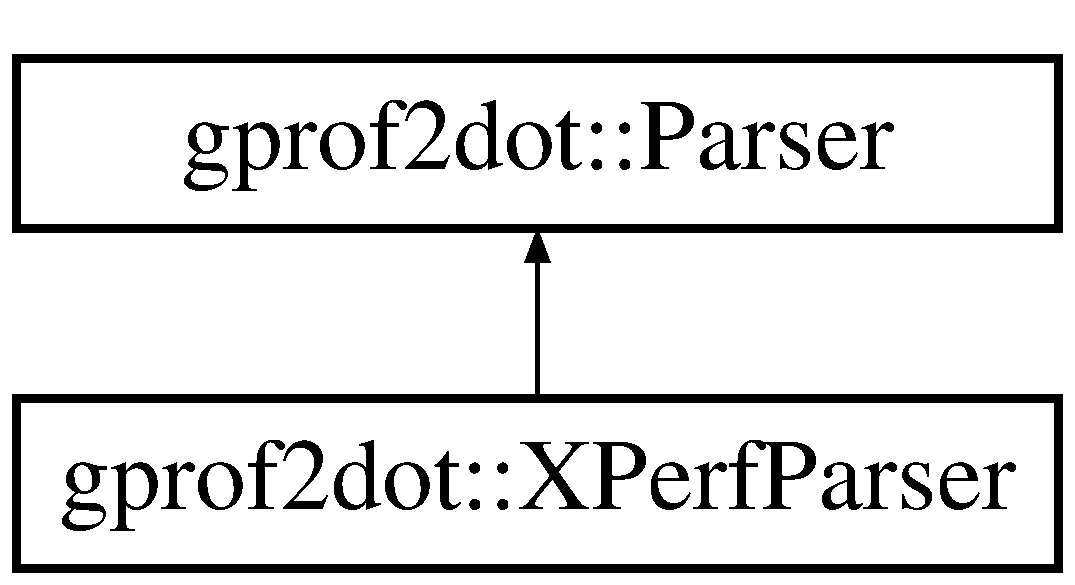
\includegraphics[height=2.000000cm]{classgprof2dot_1_1XPerfParser}
\end{center}
\end{figure}
\subsection*{Public Member Functions}
\begin{DoxyCompactItemize}
\item 
def \hyperlink{classgprof2dot_1_1XPerfParser_a2e75d52bbd69196a7d2a11f341ef9cb1}{\_\-\_\-init\_\-\_\-}
\item 
def \hyperlink{classgprof2dot_1_1XPerfParser_ac98402f482a2413c430558a01f51a75d}{parse}
\item 
def \hyperlink{classgprof2dot_1_1XPerfParser_a76edfcf4cbc019334f2f425d45d08f4c}{parse\_\-header}
\item 
def \hyperlink{classgprof2dot_1_1XPerfParser_a02c38fcf20c568d1b1dca4fae0bf457a}{parse\_\-row}
\item 
def \hyperlink{classgprof2dot_1_1XPerfParser_ab2dfe407d54dad8051e369749d674da5}{get\_\-function}
\end{DoxyCompactItemize}
\subsection*{Public Attributes}
\begin{DoxyCompactItemize}
\item 
\hyperlink{classgprof2dot_1_1XPerfParser_a5416921e1c88257c3d5e642cb0b07606}{stream}
\item 
\hyperlink{classgprof2dot_1_1XPerfParser_a549ac9abfd65063c30bc9983d6bc42ac}{profile}
\item 
\hyperlink{classgprof2dot_1_1XPerfParser_a3fd7c0ff5c2720cfd9fc8bd3ed3615b4}{column}
\end{DoxyCompactItemize}


\subsection{Detailed Description}
\begin{DoxyVerb}Parser for CSVs generted by XPerf, from Microsoft Windows Performance Tools.
\end{DoxyVerb}
 

\subsection{Constructor \& Destructor Documentation}
\hypertarget{classgprof2dot_1_1XPerfParser_a2e75d52bbd69196a7d2a11f341ef9cb1}{
\index{gprof2dot::XPerfParser@{gprof2dot::XPerfParser}!\_\-\_\-init\_\-\_\-@{\_\-\_\-init\_\-\_\-}}
\index{\_\-\_\-init\_\-\_\-@{\_\-\_\-init\_\-\_\-}!gprof2dot::XPerfParser@{gprof2dot::XPerfParser}}
\subsubsection[{\_\-\_\-init\_\-\_\-}]{\setlength{\rightskip}{0pt plus 5cm}def gprof2dot::XPerfParser::\_\-\_\-init\_\-\_\- (
\begin{DoxyParamCaption}
\item[{}]{self, }
\item[{}]{stream}
\end{DoxyParamCaption}
)}}
\label{classgprof2dot_1_1XPerfParser_a2e75d52bbd69196a7d2a11f341ef9cb1}


\subsection{Member Function Documentation}
\hypertarget{classgprof2dot_1_1XPerfParser_ab2dfe407d54dad8051e369749d674da5}{
\index{gprof2dot::XPerfParser@{gprof2dot::XPerfParser}!get\_\-function@{get\_\-function}}
\index{get\_\-function@{get\_\-function}!gprof2dot::XPerfParser@{gprof2dot::XPerfParser}}
\subsubsection[{get\_\-function}]{\setlength{\rightskip}{0pt plus 5cm}def gprof2dot::XPerfParser::get\_\-function (
\begin{DoxyParamCaption}
\item[{}]{self, }
\item[{}]{process, }
\item[{}]{symbol}
\end{DoxyParamCaption}
)}}
\label{classgprof2dot_1_1XPerfParser_ab2dfe407d54dad8051e369749d674da5}
\hypertarget{classgprof2dot_1_1XPerfParser_ac98402f482a2413c430558a01f51a75d}{
\index{gprof2dot::XPerfParser@{gprof2dot::XPerfParser}!parse@{parse}}
\index{parse@{parse}!gprof2dot::XPerfParser@{gprof2dot::XPerfParser}}
\subsubsection[{parse}]{\setlength{\rightskip}{0pt plus 5cm}def gprof2dot::XPerfParser::parse (
\begin{DoxyParamCaption}
\item[{}]{self}
\end{DoxyParamCaption}
)}}
\label{classgprof2dot_1_1XPerfParser_ac98402f482a2413c430558a01f51a75d}


Reimplemented from \hyperlink{classgprof2dot_1_1Parser_a681a0bc74e640c9c8e3d629dd03049fc}{gprof2dot::Parser}.

\hypertarget{classgprof2dot_1_1XPerfParser_a76edfcf4cbc019334f2f425d45d08f4c}{
\index{gprof2dot::XPerfParser@{gprof2dot::XPerfParser}!parse\_\-header@{parse\_\-header}}
\index{parse\_\-header@{parse\_\-header}!gprof2dot::XPerfParser@{gprof2dot::XPerfParser}}
\subsubsection[{parse\_\-header}]{\setlength{\rightskip}{0pt plus 5cm}def gprof2dot::XPerfParser::parse\_\-header (
\begin{DoxyParamCaption}
\item[{}]{self, }
\item[{}]{row}
\end{DoxyParamCaption}
)}}
\label{classgprof2dot_1_1XPerfParser_a76edfcf4cbc019334f2f425d45d08f4c}
\hypertarget{classgprof2dot_1_1XPerfParser_a02c38fcf20c568d1b1dca4fae0bf457a}{
\index{gprof2dot::XPerfParser@{gprof2dot::XPerfParser}!parse\_\-row@{parse\_\-row}}
\index{parse\_\-row@{parse\_\-row}!gprof2dot::XPerfParser@{gprof2dot::XPerfParser}}
\subsubsection[{parse\_\-row}]{\setlength{\rightskip}{0pt plus 5cm}def gprof2dot::XPerfParser::parse\_\-row (
\begin{DoxyParamCaption}
\item[{}]{self, }
\item[{}]{row}
\end{DoxyParamCaption}
)}}
\label{classgprof2dot_1_1XPerfParser_a02c38fcf20c568d1b1dca4fae0bf457a}


\subsection{Member Data Documentation}
\hypertarget{classgprof2dot_1_1XPerfParser_a3fd7c0ff5c2720cfd9fc8bd3ed3615b4}{
\index{gprof2dot::XPerfParser@{gprof2dot::XPerfParser}!column@{column}}
\index{column@{column}!gprof2dot::XPerfParser@{gprof2dot::XPerfParser}}
\subsubsection[{column}]{\setlength{\rightskip}{0pt plus 5cm}{\bf gprof2dot::XPerfParser::column}}}
\label{classgprof2dot_1_1XPerfParser_a3fd7c0ff5c2720cfd9fc8bd3ed3615b4}
\hypertarget{classgprof2dot_1_1XPerfParser_a549ac9abfd65063c30bc9983d6bc42ac}{
\index{gprof2dot::XPerfParser@{gprof2dot::XPerfParser}!profile@{profile}}
\index{profile@{profile}!gprof2dot::XPerfParser@{gprof2dot::XPerfParser}}
\subsubsection[{profile}]{\setlength{\rightskip}{0pt plus 5cm}{\bf gprof2dot::XPerfParser::profile}}}
\label{classgprof2dot_1_1XPerfParser_a549ac9abfd65063c30bc9983d6bc42ac}
\hypertarget{classgprof2dot_1_1XPerfParser_a5416921e1c88257c3d5e642cb0b07606}{
\index{gprof2dot::XPerfParser@{gprof2dot::XPerfParser}!stream@{stream}}
\index{stream@{stream}!gprof2dot::XPerfParser@{gprof2dot::XPerfParser}}
\subsubsection[{stream}]{\setlength{\rightskip}{0pt plus 5cm}{\bf gprof2dot::XPerfParser::stream}}}
\label{classgprof2dot_1_1XPerfParser_a5416921e1c88257c3d5e642cb0b07606}


The documentation for this class was generated from the following file:\begin{DoxyCompactItemize}
\item 
\hyperlink{gprof2dot_8py}{gprof2dot.py}\end{DoxyCompactItemize}

\chapter{File Documentation}
\hypertarget{Builtin_8cpp}{
\section{Builtin.cpp File Reference}
\label{Builtin_8cpp}\index{Builtin.cpp@{Builtin.cpp}}
}
{\ttfamily \#include \char`\"{}Builtin.hpp\char`\"{}}\par
{\ttfamily \#include $<$unistd.h$>$}\par
{\ttfamily \#include $<$iostream$>$}\par
{\ttfamily \#include $<$list$>$}\par
{\ttfamily \#include \char`\"{}MyTypo.hpp\char`\"{}}\par
{\ttfamily \#include $<$cstdio$>$}\par
{\ttfamily \#include $<$cstdlib$>$}\par
{\ttfamily \#include $<$signal.h$>$}\par
{\ttfamily \#include $<$sys/types.h$>$}\par
{\ttfamily \#include $<$sys/wait.h$>$}\par
{\ttfamily \#include \char`\"{}Handlers.hpp\char`\"{}}\par

\hypertarget{Builtin_8hpp}{
\section{Builtin.hpp File Reference}
\label{Builtin_8hpp}\index{Builtin.hpp@{Builtin.hpp}}
}
{\ttfamily \#include \char`\"{}Executor.hpp\char`\"{}}\par
\subsection*{Classes}
\begin{DoxyCompactItemize}
\item 
class \hyperlink{classBuiltin}{Builtin}
\begin{DoxyCompactList}\small\item\em Classe abstrata para comandos Built-\/In. \item\end{DoxyCompactList}\item 
class \hyperlink{classCdCommand}{CdCommand}
\begin{DoxyCompactList}\small\item\em Classe que implementa o comando cd. Sintaxe: cd $<$diretorio$>$ \item\end{DoxyCompactList}\item 
class \hyperlink{classPwdCommand}{PwdCommand}
\begin{DoxyCompactList}\small\item\em Classe que implementa o comando pwd. Sintaxe: pwd. \item\end{DoxyCompactList}\item 
class \hyperlink{classBgCommand}{BgCommand}
\begin{DoxyCompactList}\small\item\em Classe que implementa o comando bg. Sintaxe: bg \%$<$JOBID$>$ $|$ bg. \item\end{DoxyCompactList}\item 
class \hyperlink{classFgCommand}{FgCommand}
\begin{DoxyCompactList}\small\item\em Classe que implementa o comando fg. Sintaxe: fg \%$<$JOBID$>$ $|$ fg. \item\end{DoxyCompactList}\item 
class \hyperlink{classJobsCommand}{JobsCommand}
\begin{DoxyCompactList}\small\item\em Classe que implementa o comando jobs. Sintaxe: jobs. \item\end{DoxyCompactList}\item 
class \hyperlink{classExitCommand}{ExitCommand}
\begin{DoxyCompactList}\small\item\em Classe que implementa o comando exit. Sintaxe: exit, quit. \item\end{DoxyCompactList}\item 
class \hyperlink{classKillCommand}{KillCommand}
\begin{DoxyCompactList}\small\item\em Classe que implementa o comando kill. Sintaxe: kill \%$<$JOBID$>$ \item\end{DoxyCompactList}\end{DoxyCompactItemize}

\hypertarget{Command_8cpp}{
\section{Command.cpp File Reference}
\label{Command_8cpp}\index{Command.cpp@{Command.cpp}}
}
{\ttfamily \#include \char`\"{}Command.hpp\char`\"{}}\par

\hypertarget{Command_8hpp}{
\section{Command.hpp File Reference}
\label{Command_8hpp}\index{Command.hpp@{Command.hpp}}
}
{\ttfamily \#include $<$string$>$}\par
{\ttfamily \#include $<$vector$>$}\par
\subsection*{Classes}
\begin{DoxyCompactItemize}
\item 
class \hyperlink{classCommand}{Command}
\begin{DoxyCompactList}\small\item\em Representa um comando entrado pelo usuario. O comando representa tudo que esta numa linha ou antes de um \&. \item\end{DoxyCompactList}\end{DoxyCompactItemize}

\hypertarget{CommandLine_8cpp}{
\section{CommandLine.cpp File Reference}
\label{CommandLine_8cpp}\index{CommandLine.cpp@{CommandLine.cpp}}
}
{\ttfamily \#include \char`\"{}CommandLine.hpp\char`\"{}}\par

\hypertarget{CommandLine_8hpp}{
\section{CommandLine.hpp File Reference}
\label{CommandLine_8hpp}\index{CommandLine.hpp@{CommandLine.hpp}}
}
{\ttfamily \#include \char`\"{}Command.hpp\char`\"{}}\par
{\ttfamily \#include $<$list$>$}\par
{\ttfamily \#include $<$string$>$}\par
\subsection*{Classes}
\begin{DoxyCompactItemize}
\item 
class \hyperlink{classCommandLine}{CommandLine}
\end{DoxyCompactItemize}

\hypertarget{Executor_8cpp}{
\section{Executor.cpp File Reference}
\label{Executor_8cpp}\index{Executor.cpp@{Executor.cpp}}
}
{\ttfamily \#include \char`\"{}Executor.hpp\char`\"{}}\par
{\ttfamily \#include $<$unistd.h$>$}\par
{\ttfamily \#include $<$fcntl.h$>$}\par
{\ttfamily \#include $<$cstdio$>$}\par
{\ttfamily \#include $<$sys/stat.h$>$}\par
{\ttfamily \#include $<$sys/wait.h$>$}\par
{\ttfamily \#include $<$sys/types.h$>$}\par
{\ttfamily \#include $<$iostream$>$}\par
{\ttfamily \#include $<$cstdlib$>$}\par
{\ttfamily \#include $<$utility$>$}\par
{\ttfamily \#include \char`\"{}MyTypo.hpp\char`\"{}}\par
{\ttfamily \#include \char`\"{}Handlers.hpp\char`\"{}}\par

\hypertarget{Executor_8hpp}{
\section{Executor.hpp File Reference}
\label{Executor_8hpp}\index{Executor.hpp@{Executor.hpp}}
}
{\ttfamily \#include $<$string$>$}\par
{\ttfamily \#include $<$vector$>$}\par
{\ttfamily \#include $<$list$>$}\par
{\ttfamily \#include $<$sys/types.h$>$}\par
{\ttfamily \#include \char`\"{}Command.hpp\char`\"{}}\par
{\ttfamily \#include \char`\"{}CommandLine.hpp\char`\"{}}\par
{\ttfamily \#include $<$termios.h$>$}\par
{\ttfamily \#include \char`\"{}Builtin.hpp\char`\"{}}\par
{\ttfamily \#include $<$map$>$}\par
\subsection*{Classes}
\begin{DoxyCompactItemize}
\item 
class \hyperlink{classExecutor}{Executor}
\begin{DoxyCompactList}\small\item\em Responsavel pela execucao. Executa uma linha de comando. \item\end{DoxyCompactList}\item 
struct \hyperlink{structExecutor_1_1Job}{Executor::Job}
\end{DoxyCompactItemize}

\hypertarget{gprof2dot_8py}{
\section{gprof2dot.py File Reference}
\label{gprof2dot_8py}\index{gprof2dot.py@{gprof2dot.py}}
}
\subsection*{Classes}
\begin{DoxyCompactItemize}
\item 
class \hyperlink{classgprof2dot_1_1UndefinedEvent}{gprof2dot::UndefinedEvent}
\item 
class \hyperlink{classgprof2dot_1_1Event}{gprof2dot::Event}
\item 
class \hyperlink{classgprof2dot_1_1Object}{gprof2dot::Object}
\item 
class \hyperlink{classgprof2dot_1_1Call}{gprof2dot::Call}
\item 
class \hyperlink{classgprof2dot_1_1Function}{gprof2dot::Function}
\item 
class \hyperlink{classgprof2dot_1_1Cycle}{gprof2dot::Cycle}
\item 
class \hyperlink{classgprof2dot_1_1Profile}{gprof2dot::Profile}
\item 
class \hyperlink{classgprof2dot_1_1Struct}{gprof2dot::Struct}
\item 
class \hyperlink{classgprof2dot_1_1ParseError}{gprof2dot::ParseError}
\item 
class \hyperlink{classgprof2dot_1_1Parser}{gprof2dot::Parser}
\item 
class \hyperlink{classgprof2dot_1_1LineParser}{gprof2dot::LineParser}
\item 
class \hyperlink{classgprof2dot_1_1XmlToken}{gprof2dot::XmlToken}
\item 
class \hyperlink{classgprof2dot_1_1XmlTokenizer}{gprof2dot::XmlTokenizer}
\item 
class \hyperlink{classgprof2dot_1_1XmlTokenMismatch}{gprof2dot::XmlTokenMismatch}
\item 
class \hyperlink{classgprof2dot_1_1XmlParser}{gprof2dot::XmlParser}
\item 
class \hyperlink{classgprof2dot_1_1GprofParser}{gprof2dot::GprofParser}
\item 
class \hyperlink{classgprof2dot_1_1CallgrindParser}{gprof2dot::CallgrindParser}
\item 
class \hyperlink{classgprof2dot_1_1PerfParser}{gprof2dot::PerfParser}
\item 
class \hyperlink{classgprof2dot_1_1OprofileParser}{gprof2dot::OprofileParser}
\item 
class \hyperlink{classgprof2dot_1_1HProfParser}{gprof2dot::HProfParser}
\item 
class \hyperlink{classgprof2dot_1_1SysprofParser}{gprof2dot::SysprofParser}
\item 
class \hyperlink{classgprof2dot_1_1SharkParser}{gprof2dot::SharkParser}
\item 
class \hyperlink{classgprof2dot_1_1XPerfParser}{gprof2dot::XPerfParser}
\item 
class \hyperlink{classgprof2dot_1_1SleepyParser}{gprof2dot::SleepyParser}
\item 
class \hyperlink{classgprof2dot_1_1AQtimeTable}{gprof2dot::AQtimeTable}
\item 
class \hyperlink{classgprof2dot_1_1AQtimeParser}{gprof2dot::AQtimeParser}
\item 
class \hyperlink{classgprof2dot_1_1PstatsParser}{gprof2dot::PstatsParser}
\item 
class \hyperlink{classgprof2dot_1_1Theme}{gprof2dot::Theme}
\item 
class \hyperlink{classgprof2dot_1_1DotWriter}{gprof2dot::DotWriter}
\item 
class \hyperlink{classgprof2dot_1_1Main}{gprof2dot::Main}
\end{DoxyCompactItemize}
\subsection*{Namespaces}
\begin{DoxyCompactItemize}
\item 
namespace \hyperlink{namespacegprof2dot}{gprof2dot}
\end{DoxyCompactItemize}
\subsection*{Functions}
\begin{DoxyCompactItemize}
\item 
def \hyperlink{namespacegprof2dot_ab09acfc238bb48c2a9367a99ad646371}{gprof2dot::times}
\item 
def \hyperlink{namespacegprof2dot_a4593a742915303b1fc39347fb781b2ef}{gprof2dot::percentage}
\item 
def \hyperlink{namespacegprof2dot_aa203a76e6049687c1e57913af63d088b}{gprof2dot::add}
\item 
def \hyperlink{namespacegprof2dot_ae4ff6a99d7012515570b8258416699b0}{gprof2dot::equal}
\item 
def \hyperlink{namespacegprof2dot_aab854bd72a6622f45b68b64cdc674ba0}{gprof2dot::fail}
\item 
def \hyperlink{namespacegprof2dot_a4c10337c274ef0696d2b44a06764bf2b}{gprof2dot::ratio}
\end{DoxyCompactItemize}
\subsection*{Variables}
\begin{DoxyCompactItemize}
\item 
string \hyperlink{namespacegprof2dot_aef49cc0d071a48c27f269b1fefa0b259}{gprof2dot::\_\-\_\-author\_\-\_\-} = \char`\"{}Jose Fonseca\char`\"{}
\item 
string \hyperlink{namespacegprof2dot_abb4ac492c5f33eb464efcdd38c8a4af0}{gprof2dot::\_\-\_\-version\_\-\_\-} = \char`\"{}1.0\char`\"{}
\item 
int \hyperlink{namespacegprof2dot_a442824fd8acb25239ae698ca2c7e08d6}{gprof2dot::tol} = 2
\item 
tuple \hyperlink{namespacegprof2dot_a3cfb98044f99cfdfb0cef686b3ed3c74}{gprof2dot::CALLS} = Event(\char`\"{}Calls\char`\"{}, 0, add, times)
\item 
tuple \hyperlink{namespacegprof2dot_a4e4ea28f29d46701235f133af771103f}{gprof2dot::SAMPLES} = Event(\char`\"{}Samples\char`\"{}, 0, add)
\item 
tuple \hyperlink{namespacegprof2dot_a58b6460141073b790688ed1dd4d427ee}{gprof2dot::SAMPLES2} = Event(\char`\"{}Samples\char`\"{}, 0, add)
\item 
tuple \hyperlink{namespacegprof2dot_a6d330baab773f0f34c75fa91c763cbd3}{gprof2dot::TIME} = Event(\char`\"{}Time\char`\"{}, 0.0, add, lambda x: '(' + str(x) + ')')
\item 
tuple \hyperlink{namespacegprof2dot_ac93e094e954c5b58088dc398a764670b}{gprof2dot::TIME\_\-RATIO} = Event(\char`\"{}Time ratio\char`\"{}, 0.0, add, lambda x: '(' + percentage(x) + ')')
\item 
tuple \hyperlink{namespacegprof2dot_a3b63ba497b1ebe0c63064d7c77123930}{gprof2dot::TOTAL\_\-TIME} = Event(\char`\"{}Total time\char`\"{}, 0.0, fail)
\item 
tuple \hyperlink{namespacegprof2dot_a09afab61d414ac377c75fc45a6ea503e}{gprof2dot::TOTAL\_\-TIME\_\-RATIO} = Event(\char`\"{}Total time ratio\char`\"{}, 0.0, fail, percentage)
\item 
tuple \hyperlink{namespacegprof2dot_a4e72c47d6d17a030a03d562812c1a32a}{gprof2dot::TEMPERATURE\_\-COLORMAP}
\item 
tuple \hyperlink{namespacegprof2dot_ac297cc5a9b66874d10fdf32f4fe69417}{gprof2dot::PINK\_\-COLORMAP}
\item 
tuple \hyperlink{namespacegprof2dot_af6ef5bd07ae324a28a57189c326a514b}{gprof2dot::GRAY\_\-COLORMAP}
\item 
tuple \hyperlink{namespacegprof2dot_a7f79294d4643a0627ba9548bcce0da5b}{gprof2dot::BW\_\-COLORMAP}
\end{DoxyCompactItemize}

\hypertarget{Handlers_8cpp}{
\section{Handlers.cpp File Reference}
\label{Handlers_8cpp}\index{Handlers.cpp@{Handlers.cpp}}
}
{\ttfamily \#include \char`\"{}Handlers.hpp\char`\"{}}\par
{\ttfamily \#include $<$iostream$>$}\par
\subsection*{Variables}
\begin{DoxyCompactItemize}
\item 
bool \hyperlink{Handlers_8cpp_af95060d845619db35a3df2de559006c6}{deathStatus} = false
\end{DoxyCompactItemize}


\subsection{Variable Documentation}
\hypertarget{Handlers_8cpp_af95060d845619db35a3df2de559006c6}{
\index{Handlers.cpp@{Handlers.cpp}!deathStatus@{deathStatus}}
\index{deathStatus@{deathStatus}!Handlers.cpp@{Handlers.cpp}}
\subsubsection[{deathStatus}]{\setlength{\rightskip}{0pt plus 5cm}bool {\bf deathStatus} = false}}
\label{Handlers_8cpp_af95060d845619db35a3df2de559006c6}

\hypertarget{Handlers_8hpp}{
\section{Handlers.hpp File Reference}
\label{Handlers_8hpp}\index{Handlers.hpp@{Handlers.hpp}}
}
\subsection*{Namespaces}
\begin{DoxyCompactItemize}
\item 
namespace \hyperlink{namespacehandlers}{handlers}
\end{DoxyCompactItemize}
\subsection*{Functions}
\begin{DoxyCompactItemize}
\item 
void \hyperlink{namespacehandlers_aa02fd1a028b7cfc01ccb52b9f70cb624}{handlers::sigChildHandler} (int)
\begin{DoxyCompactList}\small\item\em Handler para SIGCHLD. Levanta uma flag dizendo que um sinal vindo de um provesso filho foi lancado. \item\end{DoxyCompactList}\item 
bool \hyperlink{namespacehandlers_a7f732d800eb51bf0ee24d554ce770276}{handlers::getDeathStatus} ()
\item 
void \hyperlink{namespacehandlers_a254dfa6abeed4136e566fd013aa9fdc4}{handlers::setDeathStatusFalse} ()
\begin{DoxyCompactList}\small\item\em Altera a flag de sinais recebidos. Altera o valor da flag de sinais recebidos para false. \item\end{DoxyCompactList}\item 
void \hyperlink{namespacehandlers_a06dc78ff46f5dcc7fb9c09a495caf4ff}{handlers::setDeathStatusTrue} ()
\begin{DoxyCompactList}\small\item\em Altera a flag de sinais recebidos. Altera o valor da flag de sinais recebidos para true. \item\end{DoxyCompactList}\end{DoxyCompactItemize}

\hypertarget{main_8cpp}{
\section{main.cpp File Reference}
\label{main_8cpp}\index{main.cpp@{main.cpp}}
}
{\ttfamily \#include \char`\"{}Program.hpp\char`\"{}}\par
\subsection*{Functions}
\begin{DoxyCompactItemize}
\item 
int \hyperlink{main_8cpp_a840291bc02cba5474a4cb46a9b9566fe}{main} (void)
\end{DoxyCompactItemize}


\subsection{Function Documentation}
\hypertarget{main_8cpp_a840291bc02cba5474a4cb46a9b9566fe}{
\index{main.cpp@{main.cpp}!main@{main}}
\index{main@{main}!main.cpp@{main.cpp}}
\subsubsection[{main}]{\setlength{\rightskip}{0pt plus 5cm}int main (
\begin{DoxyParamCaption}
\item[{void}]{}
\end{DoxyParamCaption}
)}}
\label{main_8cpp_a840291bc02cba5474a4cb46a9b9566fe}

\hypertarget{MyTypo_8cpp}{
\section{MyTypo.cpp File Reference}
\label{MyTypo_8cpp}\index{MyTypo.cpp@{MyTypo.cpp}}
}
{\ttfamily \#include \char`\"{}MyTypo.hpp\char`\"{}}\par
\subsection*{Functions}
\begin{DoxyCompactItemize}
\item 
std::ostream \& \hyperlink{MyTypo_8cpp_a9dd4ca6f7c239dd6dcc2db34f2fc02c1}{operator$<$$<$} (std::ostream \&ost, \hyperlink{classMyTypo}{MyTypo} \&mt)
\end{DoxyCompactItemize}


\subsection{Function Documentation}
\hypertarget{MyTypo_8cpp_a9dd4ca6f7c239dd6dcc2db34f2fc02c1}{
\index{MyTypo.cpp@{MyTypo.cpp}!operator$<$$<$@{operator$<$$<$}}
\index{operator$<$$<$@{operator$<$$<$}!MyTypo.cpp@{MyTypo.cpp}}
\subsubsection[{operator$<$$<$}]{\setlength{\rightskip}{0pt plus 5cm}std::ostream\& operator$<$$<$ (
\begin{DoxyParamCaption}
\item[{std::ostream \&}]{ost, }
\item[{{\bf MyTypo} \&}]{mt}
\end{DoxyParamCaption}
)}}
\label{MyTypo_8cpp_a9dd4ca6f7c239dd6dcc2db34f2fc02c1}

\hypertarget{MyTypo_8hpp}{
\section{MyTypo.hpp File Reference}
\label{MyTypo_8hpp}\index{MyTypo.hpp@{MyTypo.hpp}}
}
{\ttfamily \#include $<$iostream$>$}\par
\subsection*{Classes}
\begin{DoxyCompactItemize}
\item 
class \hyperlink{classMyTypo}{MyTypo}
\end{DoxyCompactItemize}
\subsection*{Functions}
\begin{DoxyCompactItemize}
\item 
std::ostream \& \hyperlink{MyTypo_8hpp_a9dd4ca6f7c239dd6dcc2db34f2fc02c1}{operator$<$$<$} (std::ostream \&ost, \hyperlink{classMyTypo}{MyTypo} \&mt)
\end{DoxyCompactItemize}


\subsection{Function Documentation}
\hypertarget{MyTypo_8hpp_a9dd4ca6f7c239dd6dcc2db34f2fc02c1}{
\index{MyTypo.hpp@{MyTypo.hpp}!operator$<$$<$@{operator$<$$<$}}
\index{operator$<$$<$@{operator$<$$<$}!MyTypo.hpp@{MyTypo.hpp}}
\subsubsection[{operator$<$$<$}]{\setlength{\rightskip}{0pt plus 5cm}std::ostream\& operator$<$$<$ (
\begin{DoxyParamCaption}
\item[{std::ostream \&}]{ost, }
\item[{{\bf MyTypo} \&}]{mt}
\end{DoxyParamCaption}
)}}
\label{MyTypo_8hpp_a9dd4ca6f7c239dd6dcc2db34f2fc02c1}

\hypertarget{Parser_8cpp}{
\section{Parser.cpp File Reference}
\label{Parser_8cpp}\index{Parser.cpp@{Parser.cpp}}
}
{\ttfamily \#include \char`\"{}Parser.hpp\char`\"{}}\par
{\ttfamily \#include $<$iostream$>$}\par
{\ttfamily \#include $<$string$>$}\par
{\ttfamily \#include \char`\"{}Command.hpp\char`\"{}}\par
{\ttfamily \#include $<$signal.h$>$}\par

\hypertarget{Parser_8hpp}{
\section{Parser.hpp File Reference}
\label{Parser_8hpp}\index{Parser.hpp@{Parser.hpp}}
}
{\ttfamily \#include $<$string$>$}\par
{\ttfamily \#include \char`\"{}CommandLine.hpp\char`\"{}}\par
\subsection*{Classes}
\begin{DoxyCompactItemize}
\item 
class \hyperlink{classParser}{Parser}
\end{DoxyCompactItemize}

\hypertarget{Program_8cpp}{
\section{Program.cpp File Reference}
\label{Program_8cpp}\index{Program.cpp@{Program.cpp}}
}
{\ttfamily \#include $<$iostream$>$}\par
{\ttfamily \#include \char`\"{}CommandLine.hpp\char`\"{}}\par
{\ttfamily \#include \char`\"{}Parser.hpp\char`\"{}}\par
{\ttfamily \#include \char`\"{}MyTypo.hpp\char`\"{}}\par
{\ttfamily \#include \char`\"{}Executor.hpp\char`\"{}}\par
{\ttfamily \#include $<$signal.h$>$}\par
{\ttfamily \#include \char`\"{}Handlers.hpp\char`\"{}}\par
{\ttfamily \#include $<$map$>$}\par
{\ttfamily \#include \char`\"{}Builtin.hpp\char`\"{}}\par
{\ttfamily \#include \char`\"{}Program.hpp\char`\"{}}\par

\hypertarget{Program_8hpp}{
\section{Program.hpp File Reference}
\label{Program_8hpp}\index{Program.hpp@{Program.hpp}}
}
\subsection*{Classes}
\begin{DoxyCompactItemize}
\item 
class \hyperlink{classProgram}{Program}
\end{DoxyCompactItemize}

\printindex
\end{document}
